\documentclass[UTF8,11pt,openany]{ctexbook}
\usepackage[a4paper,margin=26mm]{geometry}
\usepackage{amsmath,amssymb,amsthm,graphicx,enumitem,longtable,multicol,hyperref}
\hypersetup{unicode=true,colorlinks=true,linkcolor=blue}
\newcommand{\C}{\mathbb C}
\newcommand{\R}{\mathbb R}
\newcommand{\Z}{\mathbb Z}
\newcommand{\PP}{\mathbb P}
\newcommand{\OO}{\mathcal O}
\newcommand{\MM}{\mathcal M}
\newcommand{\sourcepage}[1]{\par\smallskip{\footnotesize\textit{〔原书第 #1 页〕}}\par\smallskip}
\newcommand{\entry}[2]{\par\medskip\noindent\textbf{#1\quad #2}\quad}
\newcommand{\translatornote}[1]{\footnote{译注：#1}}
\counterwithout{section}{chapter}
\renewcommand{\thesection}{\arabic{section}}
\setlength{\emergencystretch}{3em}
\title{黎曼曲面讲义\\GTM 81\\中文译稿}
\author{Otto Forster\\英文译者：Bruce Gilligan}
\date{}
\begin{document}
\frontmatter
\maketitle
\chapter*{译稿说明}
本稿据用户提供的英文版翻译，按原书顺序逐节推进。正文采用中文，重要术语首次出现附英文；保留原书编号、数学记号及原书页码提示。六幅编号插图依据原图用TikZ重绘为矢量图，保留原有数学标记与图意。习题不附新增解答。疑似原书错误以译注说明。

本稿已译完原书三章共31节及全部习题，收入前言、第四次修订印刷补记、附录、参考文献、符号索引、人名与主题索引，以及原版出版资料和丛书目录。原书目录以本译稿自动生成的目录对应呈现；书前与书末丛书目录合并列于书末。索引中的页码保留原书页码。

本稿为完整初译稿，完成后对部分公式、编号、插图及排版进行抽查，尚未经逐句、逐公式的全书复核。具体抽查范围与修订见项目中的《校对记录》。
\chapter*{原版书名页与出版资料}
\markboth{原版书名页与出版资料}{原版书名页与出版资料}
\addcontentsline{toc}{chapter}{原版书名页与出版资料}
\begin{center}
数学研究生教材丛书，第81卷\\[1em]
编委：S. Axler、F. W. Gehring、K. A. Ribet\\[2em]
{\Large Otto Forster}\\[1em]
{\LARGE 黎曼曲面讲义}\\[1em]
英文译者：Bruce Gilligan\\附6幅插图\\[2em]
Springer\\纽约、柏林、海德堡、巴塞罗那、香港、伦敦、米兰、巴黎、新加坡、东京
\end{center}
\bigskip
\noindent\textbf{作者与英文译者地址}\par
Otto Forster：慕尼黑大学数学研究所，Theresienstrasse 39，W-8000 München 2，德意志联邦共和国。\par
Bruce Gilligan：里贾纳大学数学系，Regina, Saskatchewan, Canada S4S 0A4。
\medskip
\noindent\textbf{编委地址}\par
S. Axler：旧金山州立大学数学系，San Francisco, CA 94132, USA。\par
F. W. Gehring：密歇根大学数学系，East Hall, Ann Arbor, MI 48109, USA。\par
K. A. Ribet：加利福尼亚大学伯克利分校数学系，Berkeley, CA 94720-3840, USA。
\medskip
\noindent 1991年数学主题分类：30-01，30Fxx。
\medskip
\noindent\textbf{美国国会图书馆在版编目数据}\par
Forster, Otto, 1937--。\par
《黎曼曲面讲义》（数学研究生教材丛书；81）。德文原著 \textit{Riemannsche Flächen} 的译本。附参考文献与索引。主题：1. 黎曼曲面。I. 书名。II. 丛书。\par
QA333.F6713\quad 515'.223\quad 81-9054\quad AACR2。
\medskip
德文原版：\textit{Riemannsche Flächen}，Heidelberger Taschenbücher 第184卷，Springer，Heidelberg，1977年。\par
© 1981 Springer-Verlag New York Inc.\par
1981年第一版精装本的平装重印本。\par
保留所有权利。未经出版社书面许可，不得翻译或复制本书的全部或部分内容。出版社地址：Springer-Verlag New York Inc., 175 Fifth Avenue, New York, NY 10010, USA。\translatornote{本段为原版版权声明的翻译，属于原书内容。}\par
印次号：9\quad8\quad7\quad6\quad5\quad4。第四次修订印刷，1999年。\par
ISBN-13：978-1-4612-5963-3。电子版 ISBN-13：978-1-4612-5961-9。\par
DOI：10.1007/978-1-4612-5961-9。

\tableofcontents
\chapter*{前言}
\markboth{前言}{前言}
\addcontentsline{toc}{chapter}{前言}
\sourcepage{vii}
本书源于作者在慕尼黑大学、雷根斯堡大学和明斯特大学讲授的黎曼曲面课程。本书旨在介绍这一丰富而优美的学科，同时介绍复流形理论中的一些方法；这些方法在单复变这一特殊情形下，显得格外初等而清晰。

全书分为三章。第一章把黎曼曲面作为覆盖空间来研究，并为此介绍所需的少量拓扑学基础。随后，我们构造由函数芽的解析延拓产生的黎曼曲面，其中尤其包括代数函数的黎曼曲面。我们还较详细地研究具有特殊多值性质的解析函数，例如全纯1形式的原函数和线性微分方程的解。

第二章讨论紧黎曼曲面，介绍Riemann--Roch定理、Abel定理及Jacobi反演问题等经典主要结果。层上同调是一项重要的技术工具。不过，我们只使用第一上同调群，而这类群处理起来相对容易。依照Serre的方法，所有主要定理都从以全纯函数层为系数的第一上同调群的有限维性推导出来。这一有限维性的证明，则以非齐次Cauchy--Riemann方程的局部可解性和Schwarz引理为基础。

第三章证明单连通黎曼曲面的Riemann映射定理（亦即单值化定理），以及Behnke--Stein关于非紧黎曼曲面的主要定理，即Runge逼近定理、Mittag--Leffler定理与Weierstrass定理。为此，我们使用Perron对Dirichlet问题的解法，
\sourcepage{viii}
以及Malgrange以Weyl引理为基础证明Runge逼近定理的方法。在这一章，我们还完成了第一章开始讨论的Stein定理，即具有指定自守加项的全纯函数的存在性定理，并介绍Röhrl对非紧黎曼曲面上Riemann--Hilbert问题的解法。

我们力求把预备知识的要求降到最低，并在需要时逐步建立必要的工具。不过，仍假定读者熟悉通常各用一学期讲授的单复变函数、一般拓扑学及代数学课程的内容。除此之外，第二、三章还用到微分拓扑和泛函分析中的少量事实，这些事实集中列在附录中。本书不需要Lebesgue积分，因为只对全纯函数或可微函数（相应地，对微分形式）作积分。我们也避免不加证明地引用任何关于曲面拓扑的定理。

本书内容大致相当于三个学期的课程。不过，第二、三章只以前面各章中的部分内容为基础。因此，读者读过第1、6、9节（黎曼曲面、层和微分形式的定义）后，可以直接阅读第二章。而在第二章中，只需第12至14节的内容，就足以在第三章中处理非紧黎曼曲面的主要定理。

英文版在每节末尾增添了习题，并在第8、17、29节中补充了一些段落。此外，有关覆盖的术语也作了调整。许多认真阅读德文版的读者帮助我们消除了若干错误，谨向他们致谢；特别感谢G.~Elencwajg，他还提出了部分习题。最后，同样要感谢译者B.~Gilligan的辛勤付出。

\begin{flushright}O. FORSTER\\明斯特，1981年5月\end{flushright}
\section*{第四次修订印刷补记}
在第二次和第四次印刷时，我们改正了若干排印错误及其他错误。谨感谢B.~Gilligan、B.~Elsner和O.~Hien编制勘误表。
\begin{flushright}O. FORSTER\\1999年4月\end{flushright}

\mainmatter
\chapter{覆盖空间}
\sourcepage{1}
黎曼曲面起源于复分析，是处理多值函数问题的一种工具。这类多值函数的出现，是因为一个给定的全纯函数元素沿不同路径作解析延拓时，一般会得到该函数的不同分支。Riemann的想法是用复平面的一个多叶覆盖来代替函数的定义域。如果构造这一覆盖时，使平面上任一点上方的点数恰好等于该点处的函数元素个数，那么在这个“覆盖曲面”上，解析函数便成为单值函数。现在，忘掉这些曲面“铺展”在复平面（或黎曼球面）之上的事实，就得到抽象黎曼曲面的概念；它们可以看作单复变解析函数的自然定义域。

本章先讨论黎曼曲面的一般概念，随后从拓扑和解析两个角度研究覆盖空间。最后，把覆盖空间理论应用于解析延拓问题、代数函数黎曼曲面的构造、微分形式的积分以及线性微分方程的求解。

\section{黎曼曲面的定义}
\sourcepage{1}
本节定义黎曼曲面、其上的全纯函数和亚纯函数，以及黎曼曲面之间的全纯映射。

黎曼曲面是带有某种附加结构的二维流形，我们即将定义这种结构。众所周知，$n$维流形是一个Hausdorff拓扑空间$X$，其中每一点$a\in X$都有一个与$\R^n$中某个开子集同胚的开邻域。
\sourcepage{2}
\entry{1.1}{定义}
设$X$是二维流形。$X$上的一个\textbf{复坐标卡}（complex chart）是从开子集$U\subset X$到开子集$V\subset\C$的一个同胚$\varphi:U\to V$。称两个复坐标卡$\varphi_i:U_i\to V_i$（$i=1,2$）\textbf{全纯相容}（holomorphically compatible），如果映射
\[
\varphi_2\circ\varphi_1^{-1}:\varphi_1(U_1\cap U_2)\longrightarrow\varphi_2(U_1\cap U_2)
\]
是双全纯的（见图1）。
\begin{center}\begin{minipage}{\linewidth}\centering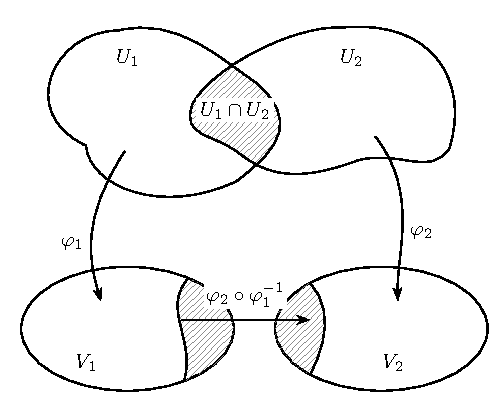
\includegraphics[width=.62\textwidth]{figures/fig01-tikz.pdf}\\图1\end{minipage}\end{center}
$X$上的一个\textbf{复图册}（complex atlas）是由彼此全纯相容的坐标卡组成的族
$\mathfrak A=\{\varphi_i:U_i\to V_i,\ i\in I\}$，并且它们覆盖$X$，即$\bigcup_{i\in I}U_i=X$。

称$X$上的两个复图册$\mathfrak A$和$\mathfrak A'$\textbf{解析等价}（analytically equivalent），如果$\mathfrak A$中的每一张坐标卡都与$\mathfrak A'$中的每一张坐标卡全纯相容。

\entry{1.2}{注记}
(a) 若$\varphi:U\to V$是复坐标卡，$U_1$是$U$中的开集，且$V_1:=\varphi(U_1)$，则$\varphi|_{U_1}:U_1\to V_1$是一张与$\varphi:U\to V$全纯相容的坐标卡。

(b) 由于双全纯映射的复合仍是双全纯映射，容易看出，复图册的解析等价关系是一个等价关系。

\entry{1.3}{定义}
二维流形$X$上的一个\textbf{复结构}（complex structure），是$X$上解析等价图册的一个等价类。

因此，选定一个复图册便可给出$X$上的一个复结构。$X$上的每个复结构$\Sigma$都包含唯一的极大图册$\mathfrak A^*$。若$\mathfrak A$是$\Sigma$中任一图册，则$\mathfrak A^*$恰由$X$上所有与$\mathfrak A$中的每张坐标卡全纯相容的复坐标卡组成。
\sourcepage{3}
\entry{1.4}{定义}
\textbf{黎曼曲面}（Riemann surface）是一个二元组$(X,\Sigma)$，其中$X$是连通二维流形，$\Sigma$是$X$上的复结构。

只要所指的复结构$\Sigma$明确，通常就写$X$而不写$(X,\Sigma)$。有时也写$(X,\mathfrak A)$，其中$\mathfrak A$是$\Sigma$的一个代表。

\textbf{约定。}若$X$是黎曼曲面，今后所说的$X$上的坐标卡，总是指属于$X$的复结构的极大图册的复坐标卡。

\textbf{注记。}局部地看，黎曼曲面$X$就是复平面中的一个开集。事实上，若$\varphi:U\to V\subset\C$是一张坐标卡，则$\varphi$把开集$U\subset X$双射到$V$。然而，$X$的任一给定点都属于许多不同的坐标卡，其中没有哪一张比其他坐标卡更特殊。因此，平面复分析中的概念，只有在双全纯映射下保持不变时，才能移植到黎曼曲面上；换言之，这些概念不能依赖某张特定坐标卡的选择。

\entry{1.5}{黎曼曲面的例子}
(a) \textbf{复平面$\C$。}它的复结构由只含恒等映射$\C\to\C$这一张坐标卡的图册定义。

(b) \textbf{区域。}设$X$是黎曼曲面，$Y\subset X$是一个区域，即连通开子集。则$Y$上存在自然的复结构，使其成为黎曼曲面：取$X$上所有满足$U\subset Y$的复坐标卡$\varphi:U\to V$作为它的图册。特别地，每个区域$Y\subset\C$都是黎曼曲面。

(c) \textbf{黎曼球面$\PP^1$。}令$\PP^1:=\C\cup\{\infty\}$，其中$\infty$是不属于$\C$的一个符号。在$\PP^1$上引入如下拓扑：开集包括$\C$中通常的开集$V$，以及形如$V\cup\{\infty\}$的集合，其中$V\subset\C$是某个紧集$K\subset\C$的补集。赋予这一拓扑后，$\PP^1$是紧Hausdorff拓扑空间，与二维球面$S^2$同胚。令
\[
U_1:=\PP^1\setminus\{\infty\}=\C,\qquad U_2:=\PP^1\setminus\{0\}=\C^*\cup\{\infty\}.
\]
如下定义映射$\varphi_i:U_i\to\C$（$i=1,2$）：$\varphi_1$是恒等映射，而
\[
\varphi_2(z):=\begin{cases}1/z,&z\in\C^*,\\0,&z=\infty.\end{cases}
\]
显然，这两个映射都是同胚，所以$\PP^1$是二维流形。又因$U_1,U_2$连通且交集非空，$\PP^1$也连通。
\sourcepage{4}
现在，由坐标卡$\varphi_i:U_i\to\C$（$i=1,2$）组成的图册定义$\PP^1$上的复结构。须证明这两张坐标卡全纯相容。但$\varphi_1(U_1\cap U_2)=\varphi_2(U_1\cap U_2)=\C^*$，且
\[
\varphi_2\circ\varphi_1^{-1}:\C^*\to\C^*,\qquad z\mapsto1/z
\]
是双全纯映射。

\textbf{注记。}记号$\PP^1$源于这样一个事实：可以把$\PP^1$看成复数域上的一维射影空间。

(d) \textbf{环面。}设$\omega_1,\omega_2\in\C$在$\R$上线性无关。定义
\[
\Gamma:=\Z\omega_1+\Z\omega_2=\{n\omega_1+m\omega_2:n,m\in\Z\}.
\]
称$\Gamma$为由$\omega_1,\omega_2$张成的\textbf{格}（lattice）（图2）。若$z-z'\in\Gamma$，则称复数$z,z'\in\C$模$\Gamma$等价。所有等价类构成的集合记为$\C/\Gamma$。令$\pi:\C\to\C/\Gamma$为典范投影，即把每一点$z\in\C$映到它模$\Gamma$的等价类的映射。
\begin{center}\begin{minipage}{\linewidth}\centering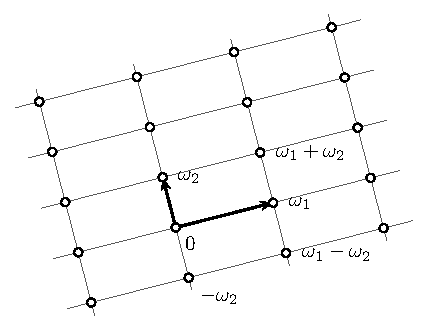
\includegraphics[width=.52\textwidth]{figures/fig02-tikz.pdf}\\图2\end{minipage}\end{center}
在$\C/\Gamma$上引入如下拓扑（商拓扑）：子集$U\subset\C/\Gamma$是开集，当且仅当$\pi^{-1}(U)\subset\C$是开集。赋予这一拓扑后，$\C/\Gamma$是Hausdorff拓扑空间，商映射$\pi:\C\to\C/\Gamma$连续。由于$\C$连通，$\C/\Gamma$也连通。此外，$\C/\Gamma$是紧的，因为紧平行四边形
\[
P:=\{\lambda\omega_1+\mu\omega_2:\lambda,\mu\in[0,1]\}
\]
在$\pi$下的像覆盖$\C/\Gamma$。映射$\pi$是开映射，即每个开集$V\subset\C$的像都是开集。为说明这一点，只须证明$\widetilde V:=\pi^{-1}(\pi(V))$是开集。但
\[
\widetilde V=\bigcup_{\omega\in\Gamma}(\omega+V).
\]
每个集合$\omega+V$都是开集，所以$\widetilde V$也是开集。
\sourcepage{5}
$\C/\Gamma$上的复结构如下定义。设$V\subset\C$是开集，且$V$中任意两点都不模$\Gamma$等价。则$U:=\pi(V)$是开集，$\pi|_V:V\to U$是同胚。它的逆映射$\varphi:U\to V$是$\C/\Gamma$上的一张复坐标卡。令$\mathfrak A$为所有以此方式得到的坐标卡所成的集合。须证明$\mathfrak A$中的任意两张坐标卡$\varphi_i:U_i\to V_i$（$i=1,2$）全纯相容。考虑映射
\[
\psi:=\varphi_2\circ\varphi_1^{-1}:\varphi_1(U_1\cap U_2)\to\varphi_2(U_1\cap U_2).
\]
对每个$z\in\varphi_1(U_1\cap U_2)$，有$\pi(\psi(z))=\varphi_1^{-1}(z)=\pi(z)$，所以$\psi(z)-z\in\Gamma$。由于$\Gamma$离散且$\psi$连续，$\psi(z)-z$在$\varphi_1(U_1\cap U_2)$的每个连通分支上都是常数。因此$\psi$全纯，同理$\psi^{-1}$也全纯。

现在赋予$\C/\Gamma$由复图册$\mathfrak A$定义的复结构。

\textbf{注记。}设$S^1=\{z\in\C:|z|=1\}$为单位圆周。把$\C/\Gamma$中由$\lambda\omega_1+\mu\omega_2$（$\lambda,\mu\in\R$）代表的点映到
\[
(e^{2\pi i\lambda},e^{2\pi i\mu})\in S^1\times S^1
\]
的映射，是$\C/\Gamma$到环面$S^1\times S^1$的同胚。

\entry{1.6}{定义}
设$X$是黎曼曲面，$Y\subset X$是开子集。称函数$f:Y\to\C$\textbf{全纯}（holomorphic），如果对$X$上的每张坐标卡$\psi:U\to V$，函数
\[
f\circ\psi^{-1}:\psi(U\cap Y)\to\C
\]
在开集$\psi(U\cap Y)\subset\C$上按通常意义全纯。$Y$上全体全纯函数构成的集合记为$\OO(Y)$。

\entry{1.7}{注记}
(a) 全纯函数的和与积仍是全纯函数，常值函数也全纯。因此$\OO(Y)$是一个$\C$代数。

(b) 当然，不必对$X$上极大图册中的所有坐标卡验证定义中的条件，只须对覆盖$Y$的任意一族坐标卡验证即可。此时其他坐标卡也自动满足这一条件。

(c) $X$上的每张坐标卡$\psi:U\to V$尤其是$U$上的一个复值函数，显然它全纯。也称$\psi$为\textbf{局部坐标}（local coordinate）或\textbf{局部一致化参数}（uniformizing parameter），并称$(U,\psi)$为任一点$a\in U$的一个\textbf{坐标邻域}（coordinate neighborhood）。在这种语境下，一般用字母$z$代替$\psi$。

\entry{1.8}{定理（Riemann可去奇点定理）}
设$U$是黎曼曲面中的开子集，$a\in U$。若函数$f\in\OO(U\setminus\{a\})$在$a$的某个邻域内有界，则$f$可唯一延拓为函数$\widetilde f\in\OO(U)$。
\sourcepage{6}
这一结果直接由复平面中的Riemann可去奇点定理得到。

现在定义黎曼曲面之间的全纯映射。

\entry{1.9}{定义}
设$X,Y$是黎曼曲面。称连续映射$f:X\to Y$\textbf{全纯}，如果对$X$上的每张坐标卡$\psi_1:U_1\to V_1$以及$Y$上的每张坐标卡$\psi_2:U_2\to V_2$，只要$f(U_1)\subset U_2$，映射
\[
\psi_2\circ f\circ\psi_1^{-1}:V_1\to V_2
\]
就按通常意义全纯。

称映射$f:X\to Y$\textbf{双全纯}（biholomorphic），如果它是双射，且$f:X\to Y$与$f^{-1}:Y\to X$都全纯。称两个黎曼曲面$X,Y$\textbf{同构}（isomorphic），如果存在双全纯映射$f:X\to Y$。

\entry{1.10}{注记}
(a) 在$Y=\C$这一特殊情形，全纯映射$f:X\to\C$显然就是全纯函数。

(b) 若$X,Y,Z$是黎曼曲面，$f:X\to Y$与$g:Y\to Z$是全纯映射，则复合$g\circ f:X\to Z$也全纯。

(c) 两个黎曼曲面之间的连续映射$f:X\to Y$全纯，当且仅当对每个开集$V\subset Y$和每个全纯函数$\psi\in\OO(V)$，“拉回”函数$\psi\circ f:f^{-1}(V)\to\C$都属于$\OO(f^{-1}(V))$。这直接由定义及注记(1.7.c)、(1.10.b)得到。

这样，全纯映射$f:X\to Y$便诱导映射
\[
f^*:\OO(V)\to\OO(f^{-1}(V)),\qquad f^*(\psi)=\psi\circ f.
\]
容易验证$f^*$是环同态。若$g:Y\to Z$是另一个全纯映射，$W$在$Z$中开，$V:=g^{-1}(W)$且$U:=f^{-1}(V)$，则$(g\circ f)^*:\OO(W)\to\OO(U)$是映射$g^*:\OO(W)\to\OO(V)$与$f^*:\OO(V)\to\OO(U)$的复合，即$(g\circ f)^*=f^*\circ g^*$。

\entry{1.11}{定理（恒等定理）}
设$X,Y$是黎曼曲面，$f_1,f_2:X\to Y$是两个全纯映射。若它们在一个具有聚点$a\in X$的集合$A\subset X$上相等，则$f_1,f_2$恒等。

\begin{proof}
令$G$为所有具有开邻域$W$使$f_1|_W=f_2|_W$的点$x\in X$所成的集合。按定义，$G$是开集。我们断言$G$也是闭集。事实上，设$b$是$G$的边界点。由$f_1,f_2$连续，有$f_1(b)=f_2(b)$。选取$X$上的坐标卡$\varphi:U\to V$和$Y$上的坐标卡$\psi:U'\to V'$，使$b\in U$且$f_i(U)\subset U'$。还可假设$U$连通。映射
\[
g_i:=\psi\circ f_i\circ\varphi^{-1}:V\to V'\subset\C
\]
\sourcepage{7}
全纯。由于$U\cap G\ne\varnothing$，由$\C$中区域上全纯函数的恒等定理可知$g_1,g_2$恒等，故$f_1|_U=f_2|_U$。于是$b\in G$，从而$G$为闭集。由于$X$连通，或者$G=\varnothing$，或者$G=X$。但再次使用平面上的恒等定理可得$a\in G$，所以第一种情况不可能。因此$f_1,f_2$在整个$X$上相等。
\end{proof}

\entry{1.12}{定义}
设$X$是黎曼曲面，$Y$是$X$的开子集。$Y$上的一个\textbf{亚纯函数}（meromorphic function）是一个全纯函数$f:Y'\to\C$，其中$Y'\subset Y$是开子集，且满足：
\begin{enumerate}[label=(\roman*)]
\item $Y\setminus Y'$只含孤立点；
\item 对每个$p\in Y\setminus Y'$，有$\displaystyle\lim_{x\to p}|f(x)|=\infty$。
\end{enumerate}
称$Y\setminus Y'$中的点为$f$的\textbf{极点}（pole）。$Y$上全体亚纯函数构成的集合记为$\MM(Y)$。

\entry{1.13}{注记}
(a) 设$(U,z)$是$f$的极点$p$的一个坐标邻域，且$z(p)=0$。则在$p$的某个邻域内，$f$可展开为Laurent级数
\[
f=\sum_{\nu=-k}^{\infty}c_\nu z^\nu,\qquad c_{-k}\ne0.
\]
(b) $\MM(Y)$具有自然的$\C$代数结构。首先，两个亚纯函数$f,g\in\MM(Y)$的和与积，在$f,g$都全纯的点处是全纯函数。然后利用Riemann可去奇点定理，将$f+g$（相应地，$fg$）越过所有可去奇点作全纯延拓。

\entry{1.14}{例}
设$n\ge1$，令
\[
F(z)=z^n+c_1z^{n-1}+\cdots+c_n
\]
为一个多项式。则$F$定义了全纯映射$F:\C\to\C$。若把$\C$视为$\PP^1$的子集，则$\lim_{z\to\infty}|F(z)|=\infty$。因此$F\in\MM(\PP^1)$。

现在把亚纯函数解释为到黎曼球面的全纯映射。

\entry{1.15}{定理}
设$X$是黎曼曲面，$f\in\MM(X)$。对$f$的每个极点$p$，定义$f(p):=\infty$。则$f:X\to\PP^1$是全纯映射。反过来，若$f:X\to\PP^1$是全纯映射，则$f$或者恒等于$\infty$，或者$f^{-1}(\infty)$只含孤立点，且$f:X\setminus f^{-1}(\infty)\to\C$是$X$上的亚纯函数。
\sourcepage{8}
今后将亚纯函数$f\in\MM(X)$与对应的全纯映射$f:X\to\PP^1$视为同一对象。
\begin{proof}
(a) 设$f\in\MM(X)$，$P$为$f$的极点集。则$f$诱导映射$f:X\to\PP^1$，它显然连续。设$\varphi:U\to V$和$\psi:U'\to V'$分别是$X$和$\PP^1$上的坐标卡，且$f(U)\subset U'$。须证明
\[
g:=\psi\circ f\circ\varphi^{-1}:V\to V'
\]
全纯。由于$f$在$X\setminus P$上全纯，$g$在$V\setminus\varphi(P)$上全纯。故由Riemann可去奇点定理，$g$在整个$V$上全纯。

(b) 逆命题由恒等定理(1.11)得到。
\end{proof}

\entry{1.16}{注记}
由(1.11)及(1.15)可知，恒等定理对黎曼曲面上的亚纯函数也成立。因此，任一不恒为零的函数$f\in\MM(X)$只有孤立零点。这表明$\MM(X)$是一个域。

\subsection*{习题（第1节）}
\entry{1.1}{}
(a) \textbf{$\R^n$的单点紧化。}设$n\ge1$，令$\infty$为不属于$\R^n$的一个符号。在集合$X:=\R^n\cup\{\infty\}$上引入如下拓扑：按定义，集合$U\subset X$为开集，当且仅当以下两个条件之一成立：
\begin{enumerate}[label=(\roman*)]
\item $\infty\notin U$，且$U$在$\R^n$的通常拓扑下是$\R^n$中的开集；
\item $\infty\in U$，且$K:=X\setminus U$在$\R^n$的通常拓扑下是紧集。
\end{enumerate}
证明$X$是紧Hausdorff拓扑空间。

(b) \textbf{球极投影。}考虑单位$n$维球面
\[
S^n=\{(x_1,\ldots,x_{n+1})\in\R^{n+1}:x_1^2+\cdots+x_{n+1}^2=1\}
\]
及球极投影$\sigma:S^n\to\R^n\cup\{\infty\}$，其定义为
\[
\sigma(x_1,\ldots,x_{n+1}):=\begin{cases}
\dfrac{1}{1-x_{n+1}}(x_1,\ldots,x_n),&x_{n+1}\ne1,\\
\infty,&x_{n+1}=1.
\end{cases}
\]
证明$\sigma$是$S^n$到$X$的同胚。

\entry{1.2}{}
设$\begin{pmatrix}a&b\\c&d\end{pmatrix}\in\operatorname{GL}(2,\C)$。
\sourcepage{9}
证明线性分式变换
\[
f(z)=\frac{az+b}{cz+d},
\]
它在$\{z\in\C:cz+d\ne0\}$上全纯，可延拓为$\PP^1$上的亚纯函数（仍记为$f$）。证明$f:\PP^1\to\PP^1$是双全纯映射，即$f$是$\PP^1$的一个自同构。

\entry{1.3}{}
利用习题1.1中定义的球极投影$\sigma:S^2\to\C\cup\{\infty\}\cong\PP^1$，把$\PP^1$与$\R^3$中的单位球面等同。设$\operatorname{SO}(3)$为行列式等于1的正交$3\times3$矩阵群，即
\[
\operatorname{SO}(3)=\{A\in\operatorname{GL}(3,\R):A^TA=1,\ \det A=1\}.
\]
对每个$A\in\operatorname{SO}(3)$，证明映射$\sigma\circ A\circ\sigma^{-1}:\PP^1\to\PP^1$是双全纯的。

［提示：利用以下事实：每个矩阵$A\in\operatorname{SO}(3)$都可写成乘积$A=A_1\cdots A_k$，其中每个$A_i$或者等于
\[
\begin{pmatrix}0&1&0\\0&0&1\\1&0&0\end{pmatrix},
\]
或者具有$\begin{pmatrix}B&0\\0&1\end{pmatrix}$的形式，其中$B\in\operatorname{SO}(2)$。］

\entry{1.4}{}
设$\Gamma=\Z\omega_1+\Z\omega_2$与$\Gamma'=\Z\omega'_1+\Z\omega'_2$是$\C$中的两个格。证明$\Gamma=\Gamma'$当且仅当存在矩阵
$A\in\operatorname{SL}(2,\Z):=\{A\in\operatorname{GL}(2,\Z):\det A=1\}$，使
\[
\begin{pmatrix}\omega'_1\\\omega'_2\end{pmatrix}
=A\begin{pmatrix}\omega_1\\\omega_2\end{pmatrix}.
\]
\translatornote{此处忠实保留原文的$\operatorname{SL}(2,\Z)$。按题面未对两组格基的定向作限制，一般应为$\operatorname{GL}(2,\Z)$，行列式可为$\pm1$；若两组格基同向，才可要求行列式为1。}

\entry{1.5}{}
(a) 设$\Gamma,\Gamma'\subset\C$是两个格。若$\alpha\in\C^*$且$\alpha\Gamma\subset\Gamma'$，证明映射$\C\to\C$，$z\mapsto\alpha z$诱导全纯映射
\[
\C/\Gamma\longrightarrow\C/\Gamma',
\]
并且该映射双全纯当且仅当$\alpha\Gamma=\Gamma'$。

(b) 证明每个环面$X=\C/\Gamma$都同构于形如
\[
X(\tau):=\C/(\Z+\Z\tau)
\]
的环面，其中$\tau\in\C$满足$\operatorname{Im}\tau>0$。

(c) 设$\begin{pmatrix}a&b\\c&d\end{pmatrix}\in\operatorname{SL}(2,\Z)$且$\operatorname{Im}\tau>0$。令$\tau':=(a\tau+b)/(c\tau+d)$。证明环面$X(\tau)$与$X(\tau')$同构。

\section{全纯映射的初等性质}
\sourcepage{10}
本节指出黎曼曲面之间全纯映射的若干初等拓扑性质。借助这些性质，可以很容易地推出复分析中的一些著名定理，例如Liouville定理和代数基本定理。

\entry{2.1}{定理（全纯映射的局部行为）}
设$X,Y$是黎曼曲面，$f:X\to Y$是非常值全纯映射。设$a\in X$且$b:=f(a)$。则存在整数$k\ge1$，以及$X$上的坐标卡$\varphi:U\to V$和$Y$上的坐标卡$\psi:U'\to V'$，满足：
\begin{enumerate}[label=(\roman*)]
\item $a\in U$，$\varphi(a)=0$；$b\in U'$，$\psi(b)=0$；
\item $f(U)\subset U'$；
\item 映射$F:=\psi\circ f\circ\varphi^{-1}:V\to V'$由$F(z)=z^k$（$z\in V$）给出。
\end{enumerate}
\begin{proof}
首先，存在$X$上的坐标卡$\varphi_1:U_1\to V_1$与$Y$上的坐标卡$\psi:U'\to V'$，使得将$(U,\varphi)$换为$(U_1,\varphi_1)$后，条件(i)、(ii)成立。由恒等定理，函数
\[
f_1:=\psi\circ f\circ\varphi_1^{-1}:V_1\to V'
\]
非常值。由于$f_1(0)=0$，存在$k\ge1$使$f_1(z)=z^kg(z)$，其中$g$在$V_1$上全纯，且$g(0)\ne0$。因此，在0的某个邻域上存在全纯函数$h$使$h^k=g$。对应$z\mapsto zh(z)$定义了一个双全纯映射$\alpha:V_2\to V$，其中$V_2\subset V_1$及$V$都是0的开邻域。令$U:=\varphi_1^{-1}(V_2)$。现在把坐标卡$\varphi_1:U_1\to V_1$换为坐标卡$\varphi:U\to V$，其中$\varphi=\alpha\circ\varphi_1$。由构造，映射$F=\psi\circ f\circ\varphi^{-1}$满足$F(z)=z^k$。
\end{proof}

\entry{2.2}{注记}
定理(2.1)中的数$k$可作如下刻画：对$a$的每个邻域$U_0$，存在$a$的邻域$U\subset U_0$与$b=f(a)$的邻域$W$，使得对每个$y\in W$、$y\ne b$，集合$f^{-1}(y)\cap U$恰含$k$个元素。称$k$为映射$f$在点$a$处取值$b$的\textbf{重数}（multiplicity），或简称$f$在点$a$处的重数为$k$。

\entry{2.3}{例}
设$f(z)=z^k+c_1z^{k-1}+\cdots+c_k$为$k$次多项式。则可把$f$看作全纯映射$f:\PP^1\to\PP^1$，其中$f(\infty)=\infty$（参见第1节）。利用$\infty$附近的坐标卡，容易验证取值$\infty$的重数为$k$。
\sourcepage{11}
\entry{2.4}{推论}
设$X,Y$是黎曼曲面，$f:X\to Y$是非常值全纯映射。则$f$是开映射，即每个开集在$f$下的像都是开集。
\begin{proof}
由定理(2.1)直接可知，若$U$是点$a\in X$的一个邻域，则$f(U)$是点$f(a)$的一个邻域。这表明$f$是开映射。
\end{proof}

\entry{2.5}{推论}
设$X,Y$是黎曼曲面，$f:X\to Y$是单射全纯映射。则$f$是$X$到$f(X)$的双全纯映射。
\begin{proof}
由于$f$单射，在定理(2.1)给出的$f$的局部描述中，总有$k=1$。因此逆映射$f^{-1}:f(X)\to X$全纯。
\end{proof}

\entry{2.6}{推论（最大值原理）}
设$X$是黎曼曲面，$f:X\to\C$是非常值全纯函数。则$f$的绝对值不取到最大值。
\begin{proof}
若存在点$a\in X$使
\[
R:=|f(a)|=\sup\{|f(x)|:x\in X\},
\]
则$f(X)\subset K:=\{z\in\C:|z|\le R\}$。由于$f(X)$是开集，它包含于$K$的内部。这与$f(a)\in\partial K$的假设矛盾。
\end{proof}

\entry{2.7}{定理}
设$X,Y$是黎曼曲面，$X$紧，且$f:X\to Y$是非常值全纯映射。则$Y$紧，且$f$为满射。
\begin{proof}
由(2.4)，$f(X)$是开集。由于$X$紧，$f(X)$紧，因而为闭集。连通拓扑空间中既开又闭的子集只有空集与全空间，所以$f(X)=Y$。因此$f$为满射，且$Y$紧。
\end{proof}

\entry{2.8}{推论}
紧黎曼曲面上的每个全纯函数都是常值函数。

由于$\C$非紧，这一结论由定理(2.7)得到。

\entry{2.9}{推论}
$\PP^1$上的每个亚纯函数$f$都是有理函数，即可写为两个多项式之商。
\sourcepage{12}
\begin{proof}
函数$f$只有有限多个极点。否则，若极点有无穷多个，它们就会有一个聚点，由恒等定理，$f$将恒等于$\infty$。可假设$\infty$不是$f$的极点；否则，以$1/f$代替$f$。设$a_1,\ldots,a_n\in\C$为$f$的极点，并设
\[
h_\nu(z)=\sum_{j=-k_\nu}^{-1}c_{\nu j}(z-a_\nu)^j
\]
为$f$在极点$a_\nu$处的主部，$\nu=1,\ldots,n$。则函数$g:=f-(h_1+\cdots+h_n)$在$\PP^1$上全纯，由推论(2.8)，它是常数。因此$f$是有理函数。
\end{proof}

\entry{2.10}{Liouville定理}
每个有界全纯函数$f:\C\to\C$都是常值函数。
\begin{proof}
由Riemann可去奇点定理(2.8)\translatornote{原文此处引用编号为(2.8)，可去奇点定理的实际编号为(1.8)。}，$f$可解析延拓为全纯映射$f:\PP^1\to\C$。由推论(2.8)，$f$为常数。
\end{proof}

\entry{2.11}{代数基本定理}
设$n\ge1$，且$f(z)=z^n+c_1z^{n-1}+\cdots+c_n$是系数$c_\nu\in\C$的多项式。则至少存在一点$a\in\C$使$f(a)=0$。
\begin{proof}
可将多项式$f$看作全纯映射$f:\PP^1\to\PP^1$，其中$f(\infty)=\infty$。由定理(2.7)，这一映射为满射，因此$0\in f(\C)$。
\end{proof}

\entry{2.12}{双周期函数}
设$\omega_1,\omega_2\in\C$在$\R$上线性无关，$\Gamma:=\Z\omega_1+\Z\omega_2$是它们张成的格。称亚纯函数$f:\C\to\PP^1$关于$\Gamma$\textbf{双周期}（doubly periodic），如果
\[
f(z)=f(z+\omega)\qquad\text{对所有 }z\in\C,\ \omega\in\Gamma.
\]
显然，只要对每个$z\in\C$有$f(z)=f(z+\omega_1)=f(z+\omega_2)$，这一条件就成立。设$\pi:\C\to\C/\Gamma$是典范映射。则双周期函数$f$诱导函数$F:\C/\Gamma\to\PP^1$，使$f=F\circ\pi$。由$\C/\Gamma$上复结构的定义直接可知，$F$是$\C/\Gamma$上的亚纯函数。反之，对任意亚纯函数$F:\C/\Gamma\to\PP^1$，复合$f=F\circ\pi:\C\to\PP^1$是关于$\Gamma$双周期的亚纯函数。因此，环面$\C/\Gamma$上的亚纯函数与$\C$上关于$\Gamma$双周期的亚纯函数一一对应。于是由定理(2.7)得到：
\sourcepage{13}
\entry{2.13}{定理}
每个双周期全纯函数$f:\C\to\C$都是常值函数。每个非常值双周期亚纯函数$f:\C\to\PP^1$都取遍所有值$c\in\PP^1$。

\subsection*{习题（第2节）}
\entry{2.1}{}
设$\Gamma\subset\C$是一个格。关于$\Gamma$的Weierstrass $\wp$函数定义为
\[
\wp_\Gamma(z)=\frac1{z^2}+\sum_{\omega\in\Gamma\setminus\{0\}}
\left(\frac1{(z-\omega)^2}-\frac1{\omega^2}\right).
\]
(a) 证明$\wp_\Gamma$是关于$\Gamma$双周期的亚纯函数，其极点位于$\Gamma$中的各点。［提示：先考虑导数
\[
\wp'_\Gamma(z)=-2\sum_{\omega\in\Gamma}\frac1{(z-\omega)^3}.
\]
］

(b) 设$f\in\MM(\C)$是关于$\Gamma$双周期的函数，其极点位于$\Gamma$中的各点，且在原点附近有如下Laurent展开：
\[
f(z)=\sum_{k=-2}^\infty c_kz^k,\qquad c_{-2}=1,\quad c_{-1}=c_0=0.
\]
证明$f=\wp_\Gamma$。

\entry{2.2}{}
设$X$是黎曼曲面，$f:X\to\C$是非常值全纯函数。证明$\operatorname{Re}f$不取到最大值。

\entry{2.3}{}
设$f:\C\to\C$是全纯函数，且其实部有上界。则$f$为常数。

\entry{2.4}{}
设$f:X\to Y$是非常值全纯映射，且
\[
f^*:\OO(Y)\to\OO(X),\qquad f^*(\varphi):=\varphi\circ f.
\]
证明$f^*$是环单同态。

\entry{2.5}{}
设$p_1,\ldots,p_n$是紧黎曼曲面$X$上的点，令$X':=X\setminus\{p_1,\ldots,p_n\}$。设$f:X'\to\C$是非常值全纯函数。证明$f$的像任意接近每个$c\in\C$。

\section{曲线的同伦·基本群}
\sourcepage{13--14}
本节介绍与曲线同伦概念有关的一些拓扑学结果。

拓扑空间$X$中的一条\textbf{曲线}是指连续映射$u:I\to X$，其中$I:=[0,1]\subset\R$为单位区间。点$a:=u(0)$称为$u$的起点，$b:=u(1)$称为终点。也称$u$为从$a$到$b$的曲线，或称曲线$u$连接$a$与$b$。

回顾：若拓扑空间$X$的任意两点$a,b$均可由曲线连接，则称$X$\textbf{弧连通}或\textbf{道路连通}（arcwise connected, pathwise connected）。弧连通空间也是连通的，即不存在$X=U_1\cup U_2$的分解，其中$U_1,U_2$为非空、不交的开集。若每一点都有由弧连通集组成的邻域基，则称空间局部弧连通。特别地，流形总满足这一条件。连通且局部弧连通的空间$X$是（整体）弧连通的，因为容易证明，所有能够与一个给定点$a\in X$用曲线连接的点$x\in X$组成的集合既开又闭。

\entry{3.1}{定义}
设$X$是拓扑空间，$a,b\in X$。称从$a$到$b$的两条曲线$u,v:I\to X$\textbf{同伦}（homotopic），记为$u\sim v$，如果存在连续映射$A:I\times I\to X$满足
\begin{enumerate}[label=(\roman*)]
\item 对每个$t\in I$，$A(t,0)=u(t)$；
\item 对每个$t\in I$，$A(t,1)=v(t)$；
\item 对每个$s\in I$，$A(0,s)=a$且$A(1,s)=b$。
\end{enumerate}
\textbf{注记。}若令$u_s(t):=A(t,s)$，则每个$u_s$都是从$a$到$b$的曲线，且$u_0=u$，$u_1=v$。曲线族$(u_s)_{0\le s\le1}$称为曲线$u$到曲线$v$的一个形变，或从$u$到$v$的一个同伦，参见图3。
\begin{center}\begin{minipage}{\linewidth}\centering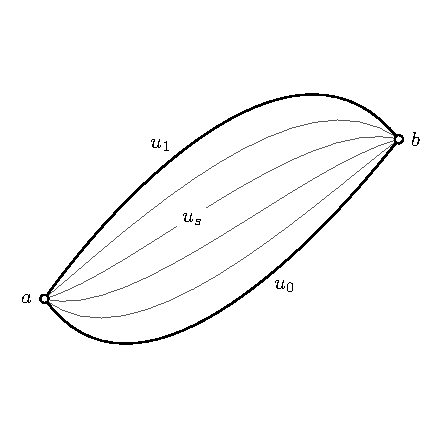
\includegraphics[width=.48\textwidth]{figures/fig03-tikz.pdf}\\图3\end{minipage}\end{center}
\entry{3.2}{定理}
设$X$是拓扑空间，$a,b\in X$。则同伦关系是从$a$到$b$的所有曲线组成的集合上的一个等价关系。
\begin{proof}
自反性和对称性显然。关于传递性，设$u,v,w:I\to X$是从$a$到$b$的三条曲线，且$u\sim v$、$v\sim w$。须证明$u\sim w$。
\sourcepage{15}
依假设，存在连续映射$A,B:I\times I\to X$，使对每个$t,s\in I$有
\begin{gather*}
A(t,0)=u(t),\quad A(t,1)=B(t,0)=v(t),\quad B(t,1)=w(t),\\
A(0,s)=B(0,s)=a,\quad A(1,s)=B(1,s)=b.
\end{gather*}
定义$C:I\times I\to X$为
\[
C(t,s):=\begin{cases}A(t,2s),&0\le s\le\tfrac12,\\B(t,2s-1),&\tfrac12\le s\le1.\end{cases}
\]
则$C$连续，是从$u$到$w$的同伦。
\end{proof}
\entry{3.3}{引理}
设$u:I\to X$是拓扑空间$X$中的曲线，$\varphi:I\to I$是满足$\varphi(0)=0$、$\varphi(1)=1$的连续映射。则曲线$u$和$u\circ\varphi$同伦。
\begin{proof}
定义$A:I\times I\to X$为$A(t,s):=u((1-s)t+s\varphi(t))$。则$A$连续，且对每个$t,s\in I$，
\[
A(t,0)=u(t),\quad A(t,1)=(u\circ\varphi)(t),\quad A(0,s)=u(0),\quad A(1,s)=u(1).
\]
因此$u$与$u\circ\varphi$同伦。
\end{proof}
\entry{3.4}{定义}
设$a,b,c$是拓扑空间$X$中的三点，$u:I\to X$是从$a$到$b$的曲线，$v:I\to X$是从$b$到$c$的曲线。

(i) 从$a$到$c$的\textbf{乘积曲线}$u\cdot v:I\to X$定义为
\[
(u\cdot v)(t):=\begin{cases}u(2t),&0\le t\le\tfrac12,\\v(2t-1),&\tfrac12\le t\le1.\end{cases}
\]
(ii) \textbf{逆曲线}$u^-:I\to X$定义为$u^-(t):=u(1-t)$（$t\in I$）。\translatornote{原文称逆曲线“从$a$到$b$”，但由定义其起点为$b$、终点为$a$。}

乘积曲线$u\cdot v$先经过曲线$u$上的点，再经过曲线$v$上的点，但速度均加倍。逆曲线$u^-$经过与$u$相同的点，方向相反。

容易验证，若$u_1,u_2:I\to X$为从$a$到$b$的同伦曲线，$v_1,v_2:I\to X$为从$b$到$c$的同伦曲线，则$u_1\cdot v_1\sim u_2\cdot v_2$，且$u_1^-\sim u_2^-$。
\sourcepage{16}
\entry{3.5}{定义}
设$X$是拓扑空间，$a\in X$。$a$处的\textbf{常曲线}是指常值映射$u_0:I\to X$，即对每个$t\in I$有$u_0(t)=a$。
\entry{3.6}{定理}
设$X$是拓扑空间，$a,b,c\in X$。设$u,v,w:I\to X$为$X$中的曲线，满足
\[
u(0)=a,\quad u(1)=b=v(0),\quad v(1)=c=w(0),\quad w(1)=d.
\]
再设$u_0$为$a$处的常曲线，$v_0$为$b$处的常曲线。则有以下同伦：
\[
\text{(i) }u_0\cdot u\sim u\sim u\cdot v_0;\qquad
\text{(ii) }u\cdot u^-\sim u_0;\qquad
\text{(iii) }(u\cdot v)\cdot w\sim u\cdot(v\cdot w).
\]
\begin{proof}
(i) 由乘积曲线的定义，
\[
(u_0\cdot u)(t)=\begin{cases}u_0(2t)=u(0),&0\le t\le\tfrac12,\\u(2t-1),&\tfrac12\le t\le1.\end{cases}
\]
故$u_0\cdot u=u\circ\psi$，其中参数变换$\psi:I\to I$在$0\le t\le\tfrac12$时为0，在$\tfrac12\le t\le1$时为$2t-1$。由引理(3.3)得$u_0\cdot u\sim u$。同理$u\cdot v_0\sim u$。

(ii) 按定义，
\[
(u\cdot u^-)(t)=\begin{cases}u(2t),&0\le t\le\tfrac12,\\u(2-2t),&\tfrac12\le t\le1.\end{cases}
\]
现在定义$A:I\times I\to X$为
\[
A(t,s):=\begin{cases}u(2t(1-s)),&0\le t\le\tfrac12,\\u(2(1-t)(1-s)),&\tfrac12\le t\le1.\end{cases}
\]
则$A$是从$u\cdot u^-$到常曲线$u_0$的同伦。

(iii) 容易验证$(u\cdot v)\cdot w=(u\cdot(v\cdot w))\circ\psi$，其中参数变换$\psi:I\to I$满足：
(a) $\psi(0)=0$，$\psi(\tfrac14)=\tfrac12$，$\psi(\tfrac12)=\tfrac34$，$\psi(1)=1$；
(b) $\psi$在$[0,\tfrac14]$、$[\tfrac14,\tfrac12]$、$[\tfrac12,1]$各区间上均为仿射线性的。由引理(3.3)即得结论。
\end{proof}
\textbf{注记。}与(iii)类似，有如下事实：若$u_1,\ldots,u_n$是$X$中的曲线，且每条$u_{k+1}$的起点等于$u_k$的终点，则对乘积$u_1\cdot u_2\cdots u_n$采用不同的加括号方式，相当于采用不同的参数变换$\psi:I\to I$，其中$\psi(0)=0$、$\psi(1)=1$。特别地，所有这些加括号方式所得曲线都同伦。
\sourcepage{17}
\entry{3.7}{定义}
称拓扑空间$X$中的曲线$u:I\to X$\textbf{闭合}，如果$u(0)=u(1)$。称起点、终点均为$a$的闭曲线$u$\textbf{零伦}（null-homotopic），如果它与$a$处的常曲线同伦。
\entry{3.8}{定理与定义}
设$X$是拓扑空间，$a\in X$。$X$中起点、终点均为$a$的闭曲线的同伦类所成的集合$\pi_1(X,a)$，在由曲线乘积诱导的运算下构成一个群。这个群称为$X$以$a$为基点的\textbf{基本群}（fundamental group）。

\textbf{记号。}任意闭曲线$u$的同伦类记为$\operatorname{cl}(u)$。按定义，$\pi_1(X,a)$中的群运算为$\operatorname{cl}(u)\operatorname{cl}(v)=\operatorname{cl}(u\cdot v)$。
\begin{proof}
群运算的良定义性由定义(3.4)末尾的注记得到。定理(3.6)说明运算满足结合律，零伦曲线的同伦类为单位元。逆元满足$\operatorname{cl}(u)^{-1}=\operatorname{cl}(u^-)$。
\end{proof}
\entry{3.9}{对基点的依赖}
设$X$是拓扑空间，点$a,b\in X$可用曲线$w$连接。如下定义映射$f:\pi_1(X,a)\to\pi_1(X,b)$：
\[
f(\operatorname{cl}(u)):=\operatorname{cl}(w^-\cdot u\cdot w).
\]
容易看出它是同构。因此，对弧连通空间$X$，基本群本质上与基点无关，往往只写$\pi_1(X)$而不写$\pi_1(X,a)$。但要注意，同构$\pi_1(X,a)\to\pi_1(X,b)$通常依赖于构造时所用的连接$a,b$的曲线$w$。若$w_1$是另一条从$a$到$b$的曲线，并定义$f_1(\operatorname{cl}(u)):=\operatorname{cl}(w_1^-\cdot u\cdot w_1)$，则自同构$F:=f_1^{-1}\circ f$满足
\[
F(\operatorname{cl}(u))=\operatorname{cl}(w_1\cdot w^-\cdot u\cdot w\cdot w_1^-),
\]
即$F(\alpha)=\gamma\cdot\alpha\cdot\gamma^{-1}$（$\alpha\in\pi_1(X,a)$），其中$\gamma$是闭曲线$w_1\cdot w^-$的同伦类。因此，若$\pi_1(X,a)$为阿贝尔群，则$\pi_1(X,a)$与$\pi_1(X,b)$典范同构。
\entry{3.10}{定义}
若弧连通拓扑空间$X$满足$\pi_1(X)=0$，则称它\textbf{单连通}（simply connected）。
\sourcepage{18}
\textbf{注记。}尽管$\pi_1(X)$的群运算用乘法记号，若$\pi_1(X)$仅含单位元，仍写$\pi_1(X)=0$。
\entry{3.11}{定理}
设$X$是弧连通且单连通的拓扑空间，$a,b\in X$。则从$a$到$b$的任意两条曲线$u,v:I\to X$同伦。
\begin{proof}
设$u_0$、$v_0$分别为$a$、$b$处的常曲线。由$\pi_1(X,b)=0$得$v^-\cdot u\sim v_0$，所以$v\cdot(v^-\cdot u)\sim v\cdot v_0$。但由定理(3.6)，
\[
v\cdot(v^-\cdot u)\sim(v\cdot v^-)\cdot u\sim u_0\cdot u\sim u,\qquad v\cdot v_0\sim v.
\]
即$u\sim v$。
\end{proof}
\entry{3.12}{例}
(a) 若对每个$x\in X\subset\R^n$，线段$\lambda a+(1-\lambda)x$（$0\le\lambda\le1$）都包含于$X$，则称$X$关于点$a\in X$\textbf{星形}。每个星形子集$X\subset\R^n$都单连通。事实上，设$u:I\to X$为起点、终点均为$a$的闭曲线，则$A:I\times I\to X$，$A(t,s):=sa+(1-s)u(t)$是从$u$到$a$处常曲线的同伦。故$\pi_1(X,a)=0$。特别地，复平面$\C$及$\C$中的每个圆盘均单连通；$\C\setminus\R_+$和$\C\setminus\R_-$也单连通，其中$\R_+$、$\R_-$分别表示正、负实半轴。

(b) 黎曼球面$\PP^1$也单连通。论证如下：令$U_1:=\PP^1\setminus\{\infty\}$，$U_2:=\PP^1\setminus\{0\}$。由于$U_1,U_2$均与$\C$同胚，故均单连通。设$u:I\to\PP^1$是任意一条从0出发又回到0的闭曲线。由$I$紧及$u$连续，可找到有限条不必闭合的曲线$u_1,\ldots,u_{2n+1}:I\to\PP^1$，满足：

(i) 乘积$v:=u_1\cdot u_2\cdots u_{2n+1}$经参数变换后等于$u$，因而与$u$同伦。

(ii) 曲线$u_{2k+1}$（$k=0,\ldots,n$）完全位于$U_1$内，曲线$u_{2k}$（$k=1,\ldots,n$）完全位于$U_2$内；$u_{2k}$的起点、终点均不等于$\infty$。

由定理(3.11)，可找到完全位于$U_2\setminus\{\infty\}$中且与$u_{2k}$同伦的曲线$u'_{2k}$。于是$v':=u_1\cdot u'_2\cdot u_3\cdot u'_4\cdots u'_{2n}\cdot u_{2n+1}$与$v$、从而与$u$同伦，并且位于$U_1$内。由$\pi_1(U_1)=0$，$v'$零伦，因此$u$也零伦。
\entry{3.13}{定义}
设$X$是拓扑空间，$u,v:I\to X$是$X$中的两条闭曲线，起点未必相同。
\sourcepage{19}
若存在连续映射$A:I\times I\to X$满足对每个$t,s\in I$有
\[
A(t,0)=u(t),\qquad A(t,1)=v(t),\qquad A(0,s)=A(1,s),
\]
则称$u,v$作为闭曲线\textbf{自由同伦}（free homotopic）。

\textbf{注记。}令$u_s(t):=A(t,s)$，则每个$u_s$都是$X$中的闭曲线，且$u_0=u$、$u_1=v$。曲线族$u_s$（$0\le s\le1$）给出从$u$到$v$的形变。令$w(t):=A(0,t)$（$0\le t\le1$），则$w$是连接$a:=u(0)=u(1)$与$b:=v(0)=v(1)$的曲线。注意，$w(s)$是曲线$u_s$的起点和终点。容易看出（参见图4），在保持起点、终点$a$不动的条件下，$u$与曲线$w\cdot v\cdot w^-$同伦。
\begin{center}\begin{minipage}{\linewidth}\centering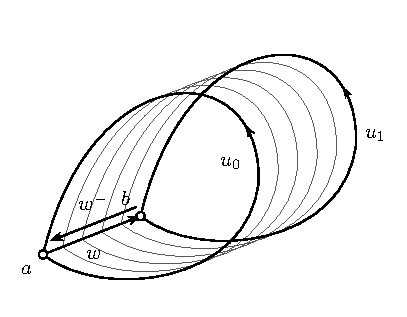
\includegraphics[width=.48\textwidth]{figures/fig04-tikz.pdf}\\图4\end{minipage}\end{center}
\entry{3.14}{定理}
道路连通拓扑空间$X$单连通，当且仅当$X$中任意两条闭曲线作为闭曲线自由同伦。

证明很简单，留给读者。
\entry{3.15}{函子性}
设$f:X\to Y$是拓扑空间之间的连续映射。若$u:I\to X$是$X$中的曲线，则$f\circ u:I\to Y$是$Y$中的曲线。若$u,u':I\to X$同伦，则$f\circ u$与$f\circ u'$也同伦。故$f$诱导基本群之间的映射
\[
f_*:\pi_1(X,a)\longrightarrow\pi_1(Y,f(a)).
\]
这一映射为群同态，因为$f\circ(u\cdot v)=(f\circ u)\cdot(f\circ v)$。若$g:Y\to Z$为另一连续映射，则$(g\circ f)_*=g_*\circ f_*$。
\subsection*{习题（第3节）}
\entry{3.1}{}
(a) 设$X$是流形，$U_1,U_2\subset X$是两个开、连通且单连通的子集，并且$U_1\cap U_2$连通。证明$U_1\cup U_2$单连通。

(b) 利用(a)证明$n\ge2$时$S^n$单连通。
\entry{3.2}{}
设$X,Y$是弧连通拓扑空间。证明$\pi_1(X\times Y)\cong\pi_1(X)\times\pi_1(Y)$。
\sourcepage{20}
\entry{3.3}{}
设$(X,a)$与$(Y,b)$是带基点的拓扑空间，$a\in X$、$b\in Y$。设$f,g:X\to Y$是两个满足$f(a)=g(a)=b$的连续映射。若存在连续映射$F:X\times[0,1]\to Y$，使对每个$x\in X$有$F(x,0)=f(x)$、$F(x,1)=g(x)$，且对每个$t\in[0,1]$有$F(a,t)=b$，则称$f,g$同伦。考虑诱导映射$f_*,g_*:\pi_1(X,a)\to\pi_1(Y,b)$。证明若$f,g$同伦，则$f_*=g_*$。

\section{分歧覆盖与无分歧覆盖}
\sourcepage{20}
黎曼曲面之间的非常值全纯映射是可能带有分歧点的覆盖映射。因此，我们现在汇集覆盖空间理论中最重要的概念与结果。
\entry{4.1}{定义}
设$X,Y$是拓扑空间，$p:Y\to X$连续。对$x\in X$，集合$p^{-1}(x)$称为$p$在$x$上的\textbf{纤维}（fiber）。若$y\in p^{-1}(x)$，则称点$y$位于$x$之上。若$p:Y\to X$、$q:Z\to X$连续，则称映射$f:Y\to Z$\textbf{保纤维}，如果$p=q\circ f$。这意味着，位于$x\in X$之上的每一点$y\in Y$，都映到仍位于$x$之上的点。

若拓扑空间的子集$A$满足每个$a\in A$都有邻域$V$使$V\cap A=\{a\}$，则称$A$\textbf{离散}。若每点$x\in X$的纤维$p^{-1}(x)$都是$Y$的离散子集，则称映射$p:Y\to X$离散。
\entry{4.2}{定理}
设$X,Y$是黎曼曲面，$p:Y\to X$是非常值全纯映射。则$p$是开的、离散的。
\begin{proof}
由(2.4)，$p$是开映射。若某点$a\in X$的纤维不离散，则由恒等定理(1.11)，$p$恒等于$a$。
\end{proof}
若$p:Y\to X$是非常值全纯映射，则称$Y$为$X$上的一个\textbf{覆盖域}（domain over $X$）。全纯函数$f:Y\to\C$（相应地，亚纯函数$f:Y\to\PP^1$）也可看作$X$上的多值全纯（亚纯）函数。若$x\in X$且$p^{-1}(x)=\{y_j:j\in J\}$，则$f(y_j)$（$j\in J$）为这一多值函数在$x$处的各个值。当然，$p^{-1}(x)$也可能只有一点或为空。
\sourcepage{21}
例如，设$Y=\C$，$X=\C^*$，$p=\exp:\C\to\C^*$。则恒等映射$\mathrm{id}:\C\to\C$对应于$\C^*$上的多值对数，因为对$b\in\C^*$，集合$\exp^{-1}(b)$恰由$b$的各个对数值组成。相应关系为
\[
\begin{array}{ccc}\C&\xrightarrow{\mathrm{id}}&\C\\ {\scriptstyle\exp}\downarrow&&\nearrow{\scriptstyle\log}\\\C^*&&\end{array}
\]
\entry{4.3}{定义}
设$X,Y$是黎曼曲面，$p:Y\to X$是非常值全纯映射。若点$y\in Y$不存在使$p|_V$单射的邻域$V$，则称$y$为$p$的\textbf{分歧点}（branch point, ramification point）。若$p$没有分歧点，则称$p$为\textbf{无分歧全纯映射}。
\entry{4.4}{定理}
黎曼曲面之间的非常值全纯映射$p:Y\to X$无分歧点，当且仅当$p$为局部同胚，即每个$y\in Y$都有开邻域$V$，使$p$将其同胚映到$X$的某个开集$U$。
\begin{proof}
若$p$无分歧点，则任意$y\in Y$都有使$p|_V$单射的开邻域$V$。由于$p$连续且为开映射，它把$V$同胚映到开集$U:=p(V)$。反之，若$p$局部同胚，则每个$y$都有被$p$同胚映到$X$中开集的开邻域$V$。特别地，$p|_V$单射，故$y$不是分歧点。
\end{proof}
\entry{4.5}{例}
(a) 设$k\ge2$为自然数，$p_k:\C\to\C$由$p_k(z):=z^k$定义。则$0\in\C$为$p_k$的分歧点，而映射$p_k|_{\C^*}:\C^*\to\C$无分歧。

(b) 设$p:Y\to X$非常值全纯，$y\in Y$，$x:=p(y)$。则$y$为$p$的分歧点，当且仅当$p$在$y$处取值$x$的重数$\ge2$，参见(2.2)。由定理(2.1)，$p$在$y$附近的局部行为，与(a)中映射$p_k$在原点附近的局部行为相同。

(c) 映射$\exp:\C\to\C^*$无分歧。因为只要子集$V\subset\C$不含相差$2\pi i$的非零整数倍的两点，$\exp$在$V$上就单射。

(d) 若$\Gamma\subset\C$为格，$\pi:\C\to\C/\Gamma$为典范商映射，参见(1.5.d)，则$\pi$无分歧。
\sourcepage{22}
\entry{4.6}{定理}
设$X$是黎曼曲面，$Y$是Hausdorff拓扑空间，$p:Y\to X$为局部同胚。则$Y$上存在唯一的复结构，使$p$全纯。

\textbf{注记。}由(2.5)，$p$甚至局部双全纯。
\begin{proof}
设$\varphi_1:U_1\to V\subset\C$是$X$的复结构的一张坐标卡，并存在开集$U\subset Y$使$p|_U:U\to U_1$为同胚。则$\varphi:=\varphi_1\circ p:U\to V$是$Y$上的复坐标卡。令$\mathfrak A$为所有如此得到的复坐标卡之集。容易看出，这些坐标卡覆盖$Y$且彼此全纯相容。赋予$Y$由$\mathfrak A$定义的复结构。则投影$p$局部双全纯，尤其全纯。

唯一性如下证明：若$\mathfrak A'$是$Y$上的另一个复图册，使$p:(Y,\mathfrak A')\to X$全纯，因而局部双全纯，则恒等映射$(Y,\mathfrak A)\to(Y,\mathfrak A')$局部双全纯，从而双全纯。因此$\mathfrak A,\mathfrak A'$定义同一复结构。
\end{proof}
\entry{4.7}{映射的提升}
设$X,Y,Z$是拓扑空间，$p:Y\to X$与$f:Z\to X$连续。$f$关于$p$的一个\textbf{提升}（lifting）是指连续映射$g:Z\to Y$，使$f=p\circ g$，即下图交换：
\[
\begin{array}{ccc} &Y&\\ {\scriptstyle g}\nearrow&&\downarrow{\scriptstyle p}\\ Z&\xrightarrow{f}&X\end{array}
\]
\entry{4.8}{定理（提升的唯一性）}
设$X,Y$是Hausdorff空间，$p:Y\to X$为局部同胚，$Z$是连通拓扑空间，$f:Z\to X$连续。若$g_1,g_2:Z\to Y$为$f$的两个提升，并在某点$z_0\in Z$处有$g_1(z_0)=g_2(z_0)$，则$g_1=g_2$。
\begin{proof}
令$T:=\{z\in Z:g_1(z)=g_2(z)\}$。由于$T$是对角线$\Delta\subset Y\times Y$在映射$(g_1,g_2):Z\to Y\times Y$下的原像，$T$为闭集。断言$T$也开。设$z\in T$，$y:=g_1(z)=g_2(z)$。由$p$局部同胚，$y$有邻域$V$被$p$同胚映到$p(y)=f(z)$的邻域$U$。由$g_1,g_2$连续，存在$z$的邻域$W$使$g_i(W)\subset V$。设$\varphi:U\to V$为$p|_V$的连续逆映射。由$p\circ g_i=f$，对$i=1,2$有$g_i|_W=\varphi\circ(f|_W)$。故$g_1|_W=g_2|_W$，$W\subset T$。因此$T$开。由$Z$连通且$T$非空，$T=Z$，即$g_1=g_2$。
\end{proof}
\sourcepage{23}
\entry{4.9}{定理}
设$X,Y,Z$是黎曼曲面，$p:Y\to X$是无分歧全纯映射，$f:Z\to X$为任意全纯映射。则$f$的每个提升$g:Z\to Y$均全纯。
\begin{proof}
任取$c\in Z$，令$b:=g(c)$、$a:=p(b)=f(c)$。存在$b$、$a$的开邻域$V,U$使$p|_V:V\to U$双全纯。设$\varphi:U\to V$为逆映射。由$g$连续，存在$c$的开邻域$W$使$g(W)\subset V$。由$f=p\circ g$得$g|_W=\varphi\circ(f|_W)$，故$g$在$c$处全纯。
\end{proof}
\textbf{推论。}若$p:Y\to X$、$q:Z\to X$是黎曼曲面之间的无分歧全纯映射，则每个连续保纤维映射$f:Y\to Z$均全纯，因为$f$是$p$关于$q$的提升。

\textbf{曲线的提升。}设$X,Y$是Hausdorff空间，$p:Y\to X$局部同胚。我们特别关心曲线$u:[0,1]\to X$的提升。由定理(4.8)，若提升$\widetilde u:[0,1]\to Y$存在，则一旦指定起点的提升，整条提升便唯一确定。下文仍令$I:=[0,1]$。
\entry{4.10}{定理（同伦曲线的提升）}
设$X,Y$是Hausdorff空间，$p:Y\to X$局部同胚。设$a,b\in X$，$\widetilde a\in Y$且$p(\widetilde a)=a$。再设给定连续映射$A:I\times I\to X$，对每个$s\in I$有$A(0,s)=a$、$A(1,s)=b$。令$u_s(t):=A(t,s)$。若每条$u_s$均可提升为以$\widetilde a$为起点的曲线$\widetilde u_s$，则$\widetilde u_0,\widetilde u_1$有相同终点，且彼此同伦。
\begin{proof}
定义$\widetilde A:I\times I\to Y$为$\widetilde A(t,s):=\widetilde u_s(t)$。

断言(a)：存在$\varepsilon_0>0$使$\widetilde A$在$[0,\varepsilon_0[\,\times I$上连续。证明：存在$\widetilde a$、$a$的邻域$V,U$使$p|_V:V\to U$同胚。令$\varphi:U\to V$为逆映射。由$A(\{0\}\times I)=\{a\}$及$A$连续，存在$\varepsilon_0>0$使$A([0,\varepsilon_0]\times I)\subset U$。由曲线提升的唯一性，对每个$s\in I$有$\widetilde u_s|_{[0,\varepsilon_0]}=\varphi\circ u_s|_{[0,\varepsilon_0]}$。故在$[0,\varepsilon_0]\times I$上$\widetilde A=\varphi\circ A$，从而连续。

断言(b)：$\widetilde A$在整个$I\times I$上连续。反设它在某点$(t_0,\sigma)$不连续。令$\tau$为使$\widetilde A$在$(t,\sigma)$处不连续的所有$t$的下确界。由(a)，$\tau\ge\varepsilon_0$。令$x:=A(\tau,\sigma)$，$y:=\widetilde A(\tau,\sigma)=\widetilde u_\sigma(\tau)$。
\sourcepage{24}
存在$y$、$x$的邻域$V,U$，使$p|_V:V\to U$为同胚。设$\varphi:U\to V$为逆。由$A$连续，存在$\varepsilon>0$使$A(I_\varepsilon(\tau)\times I_\varepsilon(\sigma))\subset U$，其中$I_\varepsilon(\xi):=\{t\in I:|t-\xi|<\varepsilon\}$。特别地，$u_\sigma(I_\varepsilon(\tau))\subset U$，故$\widetilde u_\sigma|_{I_\varepsilon(\tau)}=\varphi\circ u_\sigma|_{I_\varepsilon(\tau)}$。

选$t_1\in I_\varepsilon(\tau)$使$t_1<\tau$，则$\widetilde A(t_1,\sigma)=\widetilde u_\sigma(t_1)\in V$。由$\widetilde A$在$(t_1,\sigma)$处连续，存在$0<\delta\le\varepsilon$使对每个$s\in I_\delta(\sigma)$有$\widetilde A(t_1,s)=\widetilde u_s(t_1)\in V$。由提升唯一性，所有这些$s$均满足$\widetilde u_s|_{I_\varepsilon(\tau)}=\varphi\circ u_s|_{I_\varepsilon(\tau)}$。因此$\widetilde A=\varphi\circ A$在$I_\varepsilon(\tau)\times I_\delta(\sigma)$上成立。这与$(\tau,\sigma)$的定义矛盾。所以$\widetilde A$在$I\times I$上连续。

由$A=p\circ\widetilde A$及$A(\{1\}\times I)=\{b\}$，有$\widetilde A(\{1\}\times I)\subset p^{-1}(b)$。由于$p^{-1}(b)$离散而$\{1\}\times I$连通，其像只有一点。这说明$\widetilde u_0,\widetilde u_1$终点相同，且$\widetilde A$给出它们的同伦。
\end{proof}
\textbf{覆盖映射。}现在给出保证曲线总可提升的条件。
\entry{4.11}{定义}
设$X,Y$是拓扑空间。若映射$p:Y\to X$满足下述条件，则称为\textbf{覆盖映射}（covering map）：每个$x\in X$都有开邻域$U$，其原像可写为$p^{-1}(U)=\bigcup_{j\in J}V_j$，其中$V_j$为$Y$中两两不交的开集，且所有$p|_{V_j}:V_j\to U$均为同胚。特别地，$p$是局部同胚。
\entry{4.12}{例}
(a) 设$D=\{z\in\C:|z|<1\}$为单位圆盘，$p:D\to\C$为典范嵌入。则$p$局部同胚，却不是覆盖映射，因为每个满足$|a|=1$的点$a\in\C$均不存在符合定义要求的邻域$U$。

(b) 设$k\ge2$为自然数，令$p_k:\C^*\to\C^*$，$z\mapsto z^k$。
\sourcepage{25}
则$p_k$为覆盖映射。事实上，任取$a\in\C^*$并选$b\in\C^*$使$p_k(b)=a$。由$p_k$局部同胚，存在$b$、$a$的开邻域$V_0,U$使$p_k|_{V_0}:V_0\to U$为同胚。于是$p_k^{-1}(U)=V_0\cup\omega V_0\cup\cdots\cup\omega^{k-1}V_0$，其中$\omega$为一个$k$次本原单位根，例如$\omega=\exp(2\pi i/k)$。显然，$V_j:=\omega^jV_0$（$j=0,\ldots,k-1$）两两不交，且$p_k|_{V_j}:V_j\to U$均为同胚。

(c) 映射$\exp:\C\to\C^*$为覆盖映射。
\begin{proof}
设$a\in\C^*$，$b\in\C$且$\exp(b)=a$。由$\exp$局部同胚，存在$b$、$a$的开邻域$V_0,U$使$\exp|_{V_0}:V_0\to U$为同胚。于是$\exp^{-1}(U)=\bigcup_{n\in\Z}V_n$，其中$V_n:=2\pi in+V_0$。显然各$V_n$两两不交，每个$\exp|_{V_n}:V_n\to U$均为同胚。
\end{proof}
(d) 若$\Gamma\subset\C$为格，$\pi:\C\to\C/\Gamma$为典范商映射，则与(c)同样可证$\pi$为覆盖映射。
\entry{4.13}{定义}
若连续映射$p:Y\to X$满足下述条件，则称它具有\textbf{曲线提升性质}：对每条曲线$u:[0,1]\to X$以及每点$y_0\in Y$，只要$p(y_0)=u(0)$，就存在$u$的提升$\widetilde u:[0,1]\to Y$满足$\widetilde u(0)=y_0$。
\entry{4.14}{定理}
拓扑空间之间的每个覆盖映射$p:Y\to X$均具有曲线提升性质。
\begin{proof}
设$u:[0,1]\to X$为曲线，$p(y_0)=u(0)$。由$[0,1]$紧，存在分割$0=t_0<t_1<\cdots<t_n=1$及开集$U_k\subset X$（$k=1,\ldots,n$）满足：
(i) $u([t_{k-1},t_k])\subset U_k$；(ii) $p^{-1}(U_k)=\bigcup_{j\in J_k}V_{kj}$，其中$V_{kj}\subset Y$为开集，$p|_{V_{kj}}:V_{kj}\to U_k$是同胚。

对$k=0,1,\ldots,n$归纳构造$u|_{[0,t_k]}$的提升$\widetilde u$，使$\widetilde u(0)=y_0$。$k=0$显然。设$k\ge1$，且已构造到$[0,t_{k-1}]$，令$y_{k-1}:=\widetilde u(t_{k-1})$。由$p(y_{k-1})=u(t_{k-1})\in U_k$，存在$j\in J_k$使$y_{k-1}\in V_{kj}$。
\sourcepage{26}
令$\varphi:U_k\to V_{kj}$为$p|_{V_{kj}}$的逆。定义$\widetilde u|_{[t_{k-1},t_k]}:=\varphi\circ(u|_{[t_{k-1},t_k]})$，便得到提升到$[0,t_k]$的连续延拓。
\end{proof}
\entry{4.15}{注记}
设$X,Y$为Hausdorff空间，$p:Y\to X$为覆盖映射，$p(y_0)=x_0$。由(4.14)、(4.8)，每条以$x_0$为起点的曲线$u:[0,1]\to X$均有唯一以$y_0$为起点的提升$\widetilde u:[0,1]\to Y$。即使$u$闭合，$\widetilde u$也未必闭合。例如$X=Y=\C^*$，$p(z)=z^2$，$x_0=y_0=1$。曲线$u(t)=e^{2\pi it}$从1出发又回到1，故闭合；其提升$\widetilde u(t)=e^{\pi it}$却从1到$-1$。

不过，由定理(4.10)，闭合零伦曲线的每个提升仍闭合且零伦。
\entry{4.16}{定理}
设$X,Y$是Hausdorff空间，$X$道路连通，$p:Y\to X$为覆盖映射。则任意$x_0,x_1\in X$的纤维$p^{-1}(x_0)$、$p^{-1}(x_1)$具有相同基数。特别地，若$Y$非空，则$p$满射。

纤维$p^{-1}(x)$的基数称为覆盖的\textbf{叶数}，可以有限，也可以无限。
\begin{proof}
如下构造$\varphi:p^{-1}(x_0)\to p^{-1}(x_1)$：选连接$x_0,x_1$的曲线$u$。每个$y\in p^{-1}(x_0)$均确定唯一以$y$为起点的提升$\widetilde u$。令$\varphi(y):=\widetilde u(1)$。由提升唯一性，这一映射是双射。
\end{proof}
\textbf{注记。}证明中构造的双射通常依赖曲线$u$的选择。因此，通常无法以良定义的方式对覆盖的各“叶”作整体编号。
\entry{4.17}{定理}
设$X,Y$是Hausdorff空间，$p:Y\to X$为覆盖映射。设$Z$是单连通、道路连通且局部道路连通的拓扑空间，$f:Z\to X$连续。则对每组满足$f(z_0)=p(y_0)$的点$z_0\in Z,y_0\in Y$，恰有一个提升$\widetilde f:Z\to Y$满足$\widetilde f(z_0)=y_0$。
\sourcepage{27}
\textbf{注记。}下述证明只用到$p$是局部同胚并具有曲线提升性质。
\begin{proof}
任取$z\in Z$，选从$z_0$到$z$的曲线$u:I\to Z$。则$v:=f\circ u$从$f(z_0)$到$f(z)$。令$\widetilde v$为$v$以$y_0$为起点的唯一提升，并定义$\widetilde f(z):=\widetilde v(1)$。这与$u$的选择无关：若$u_1$也是从$z_0$到$z$的曲线，则由$Z$单连通，$u_1\sim u$，从而$v_1:=f\circ u_1\sim v$。由(4.10)，以$y_0$为起点的提升$\widetilde v_1,\widetilde v$终点相同。因此$\widetilde f$良定义，且依构造$f=p\circ\widetilde f$。

只须证明$\widetilde f$连续。设$z\in Z$、$y=\widetilde f(z)$，$V$为$y$的邻域。须找到$z$的邻域$W$使$\widetilde f(W)\subset V$。由$p$局部同胚，必要时缩小$V$，可假设$p|_V:V\to U$同胚，其中$U$为$p(y)=f(z)$的邻域。设$\varphi$为其逆。由$f$连续及$Z$局部道路连通，可选$z$的道路连通邻域$W$使$f(W)\subset U$。

断言$\widetilde f(W)\subset V$。保持上述曲线$u,v,\widetilde v$，任取$z'\in W$，选完全位于$W$内的从$z$到$z'$的曲线$u'$。则$v':=f\circ u'$位于$U$内，$\widetilde v':=\varphi\circ v'$是以$y$为起点的提升。故$\widetilde v\cdot\widetilde v'$是$v\cdot v'=f\circ(u\cdot u')$以$y_0$为起点的提升。因此$\widetilde f(z')=(\widetilde v\cdot\widetilde v')(1)=\widetilde v'(1)\in V$。唯一性由(4.8)得到。
\end{proof}
\entry{4.18}{例（函数的对数）}
设$X$是单连通黎曼曲面，$f:X\to\C^*$是处处非零的全纯函数。要找$f$的对数，即全纯函数$F:X\to\C$使$\exp(F)=f$。这恰好要求$F$是$f$关于覆盖$\exp:\C\to\C^*$的提升：
\[
\begin{array}{ccc}&\C&\\{\scriptstyle F}\nearrow&&\downarrow{\scriptstyle\exp}\\X&\xrightarrow{f}&\C^*\end{array}
\]
若$x_0\in X$，$c\in\C$为方程$e^c=f(x_0)$的任一解，则由(4.17)存在所需提升$F$且$F(x_0)=c$。由(4.9)，$F$全纯。任何其他解与$F$只差加法常数$2\pi in$（$n\in\Z$）。
\sourcepage{28}
特别地，若$X$是$\C^*$中的单连通区域，$j:X\to\C^*$为典范嵌入$j(z)=z$，则$j$关于$\exp$的每个提升恰为$\log$在$X$上的一个分支。类似地，利用例(4.12.b)的覆盖，可以在任意单连通黎曼曲面上构造处处非零全纯函数的各种根。
\entry{4.19}{定理}
设$X$是流形，$Y$是Hausdorff空间，$p:Y\to X$是具有曲线提升性质的局部同胚。则$p$为覆盖映射。
\begin{proof}
任取$x_0\in X$，设$y_j$（$j\in J$）为其全部原像。取$x_0$的开邻域$U$使其同胚于球，令$f:U\to X$为典范嵌入。由(4.17)的注记，每个$j\in J$均存在$f$的提升$\widetilde f_j:U\to Y$使$\widetilde f_j(x_0)=y_j$。令$V_j:=\widetilde f_j(U)$。容易验证$p^{-1}(U)=\bigcup_{j\in J}V_j$，各$V_j$为两两不交的开集，且每个$p|_{V_j}:V_j\to U$均为同胚。
\end{proof}
\entry{4.20}{固有映射}
回顾：局部紧拓扑空间是每点都有紧邻域的Hausdorff空间。局部紧空间之间的连续映射$f:X\to Y$称为\textbf{固有映射}（proper），如果每个紧集的原像均紧。例如，$X$紧时总成立。固有映射是闭映射，即每个闭集的像均闭。这是因为，在局部紧空间中，子集为闭集当且仅当它与每个紧集的交集均紧。
\entry{4.21}{引理}
设$X,Y$局部紧，$p:Y\to X$是固有离散映射。则：
(a) 每个$x\in X$的纤维$p^{-1}(x)$有限；
(b) 若$V$为$p^{-1}(x)$的邻域，则存在$x$的邻域$U$使$p^{-1}(U)\subset V$。
\begin{proof}
(a) $p^{-1}(x)$是紧的离散子集，因此有限。

(b) 可假设$V$开，于是$Y\setminus V$闭，$A:=p(Y\setminus V)$也闭，且$x\notin A$。因此$U:=X\setminus A$是$x$的开邻域，满足$p^{-1}(U)\subset V$。
\end{proof}
\sourcepage{29}
\entry{4.22}{定理}
设$X,Y$局部紧，$p:Y\to X$是固有局部同胚。则$p$为覆盖映射。
\begin{proof}
任取$x\in X$，令$p^{-1}(x)=\{y_1,\ldots,y_n\}$，各$y_j$互异。由$p$局部同胚，每个$y_j$都有开邻域$W_j$以及$x$的开邻域$U_j$，使$p|_{W_j}:W_j\to U_j$同胚。可令各$W_j$两两不交。由于$W_1\cup\cdots\cup W_n$为$p^{-1}(x)$的邻域，由(4.21.b)，存在$x$的开邻域$U\subset U_1\cap\cdots\cap U_n$使$p^{-1}(U)\subset W_1\cup\cdots\cup W_n$。令$V_j:=W_j\cap p^{-1}(U)$，则各$V_j$为不交开集，$p^{-1}(U)=V_1\cup\cdots\cup V_n$，且各$p|_{V_j}:V_j\to U$为同胚。
\end{proof}
\entry{4.23}{固有全纯映射}
设$f:X\to Y$为黎曼曲面之间的固有非常值全纯映射。由(2.1)，$f$的分歧点集$A$闭且离散。由$f$固有，$B:=f(A)$也闭且离散。称$B$为$f$的\textbf{临界值集}。

令$Y':=Y\setminus B$、$X':=X\setminus f^{-1}(B)\subset X\setminus A$。则$f|_{X'}:X'\to Y'$是固有无分歧全纯覆盖，由(4.22)、(4.16)、(4.21.a)，有良定义的有限叶数$n$。这意味着每个$c\in Y'$恰被取到$n$次。为把这一结论推广到临界值$b\in B$，须考虑重数。

对$x\in X$，用$\nu(f,x)$表示(2.2)意义下$f$在$x$处取值$f(x)$的重数。若$m=\sum_{x\in f^{-1}(c)}\nu(f,x)$，则称$f$在$X$上按重数计算取值$c\in Y$共$m$次。
\entry{4.24}{定理}
设$f:X\to Y$为黎曼曲面之间的固有非常值全纯映射。则存在自然数$n$，使$f$按重数计算恰取每个值$c\in Y$共$n$次。
\begin{proof}
沿用(4.23)的记号，令$n$为无分歧覆盖$f|_{X'}$的叶数。设$b\in B$为临界值，$f^{-1}(b)=\{x_1,\ldots,x_r\}$，$k_j:=\nu(f,x_j)$。由(2.1)、(2.2)，存在两两不交的$x_j$的邻域$V_j$及$b$的邻域$U_j$，使对每个$c\in U_j\setminus\{b\}$，集合$f^{-1}(c)\cap V_j$恰有$k_j$点。由(4.21.b)，可取$b$的邻域$U\subset U_1\cap\cdots\cap U_r$使$f^{-1}(U)\subset V_1\cup\cdots\cup V_r$。因此对每个$c\in U\cap Y'$，$f^{-1}(c)$有$k_1+\cdots+k_r$点。另一方面，$c\in Y'$时纤维基数为$n$，故$n=k_1+\cdots+k_r$。
\end{proof}
\sourcepage{30}
\textbf{注记。}固有非常值全纯映射称为\textbf{$n$叶全纯覆盖映射}，其中$n$为上一定理中的整数。注意，全纯覆盖映射允许有分歧点。若要强调不存在分歧点，将明确称它为无分歧映射。说到拓扑覆盖映射，或没有复结构时，指的是(4.11)意义下的覆盖映射。
\entry{4.25}{推论}
紧黎曼曲面$X$上的每个非常值亚纯函数$f:X\to\PP^1$，按重数计算，其零点个数与极点个数相同。
\begin{proof}映射$f:X\to\PP^1$是固有的。\end{proof}
\entry{4.26}{推论}
任意$n$次多项式$f(z)=z^n+a_1z^{n-1}+\cdots+a_n\in\C[z]$按重数计算恰有$n$个零点。
\begin{proof}
由(2.3)，可把$f$看作全纯映射$f:\PP^1\to\PP^1$，它按重数计算恰取值$\infty$共$n$次。
\end{proof}
\subsection*{习题（第4节）}
\entry{4.1}{}
令$X:=\C\setminus\{\pm1\}$，$Y:=\C\setminus\{\pi/2+k\pi:k\in\Z\}$。证明$\sin:Y\to X$为拓扑覆盖映射。考虑$X$中的曲线
\[
u:[0,1]\to X,\quad u(t):=1-e^{2\pi it};\qquad
v:[0,1]\to X,\quad v(t):=-1+e^{2\pi it}.
\]
设$w_1:[0,1]\to Y$为$u\cdot v$满足$w_1(0)=0$的提升，$w_2$为$v\cdot u$满足$w_2(0)=0$的提升。证明$w_1(1)=2\pi$、$w_2(1)=-2\pi$。由此推出$\pi_1(X)$不是阿贝尔群。
\entry{4.2}{}
设$X,Y$为弧连通Hausdorff拓扑空间，$f:Y\to X$为覆盖映射。证明诱导映射$f_*:\pi_1(Y)\to\pi_1(X)$为单射。
\sourcepage{31}
\entry{4.3}{}
设$X,Y$为Hausdorff空间，$p:Y\to X$为覆盖映射，$Z$为连通、局部弧连通拓扑空间，$f:Z\to X$连续。设$c\in Z$，$a:=f(c)$，$b\in Y$且$p(b)=a$。证明：存在$f$的提升$\widetilde f:Z\to Y$满足$\widetilde f(c)=b$，当且仅当$f_*\pi_1(Z,c)\subset p_*\pi_1(Y,b)$。
\entry{4.4}{}
(a) 证明$\tan:\C\to\PP^1$为局部同胚。

(b) 证明$\tan(\C)=\PP^1\setminus\{\pm i\}$，且$\tan:\C\to\PP^1\setminus\{\pm i\}$为覆盖映射。

(c) 令$X=\C\setminus\{it:t\in\R,\ |t|\ge1\}$。证明对每个$k\in\Z$，存在唯一全纯函数$\arctan_k:X\to\C$满足$\tan\circ\arctan_k=\mathrm{id}_X$及$\arctan_k(0)=k$（$\arctan$的第$k$个分支）。\translatornote{原文为$\arctan_k(0)=k$。按$\tan w=0$的解为$k\pi$，这里应为$k\pi$。}
\entry{4.5}{}
求映射$f:\C\to\PP^1$，$f(z):=\tfrac12(z+1/z)$的分歧点。

\section{万有覆盖与覆盖变换}
\sourcepage{31--32}
流形$X$的所有覆盖空间中，有一个可称为“最大”的覆盖，即万有覆盖。所有其他覆盖空间都可作为它的商得到；万有覆盖在“覆盖变换”群作用下的行为，与$X$的基本群密切相关。本节研究这些概念。
\entry{5.1}{定义}
设$X,Y$为连通拓扑空间，$p:Y\to X$为覆盖映射。若满足下述泛性质，则称$p$为$X$的\textbf{万有覆盖}（universal covering）：对每个覆盖$q:Z\to X$（$Z$连通），以及每组满足$p(y_0)=q(z_0)$的点$y_0\in Y,z_0\in Z$，恰存在一个连续保纤维映射$f:Y\to Z$使$f(y_0)=z_0$。

连通拓扑空间$X$的万有覆盖在同构意义下至多一个。事实上，沿用上述记号，若$q:Z\to X$也是万有覆盖，则存在连续保纤维映射$g:Z\to Y$满足$g(z_0)=y_0$。复合$g\circ f:Y\to Y$、$f\circ g:Z\to Z$均连续且保纤维，并分别固定$y_0,z_0$。由泛性质，每种情形满足这些条件的映射只有一个，故$g\circ f=\mathrm{id}_Y$、$f\circ g=\mathrm{id}_Z$。所以$f$是保纤维同胚。
\entry{5.2}{定理}
设$X,Y$为连通流形，$Y$单连通，$p:Y\to X$为覆盖映射。则$p$是$X$的万有覆盖。
\begin{proof}由定义及定理(4.17)直接得到。\end{proof}
\entry{5.3}{定理}
设$X$是连通流形。则存在连通、单连通流形$\widetilde X$及覆盖映射$p:\widetilde X\to X$。

由定理(5.2)，$\widetilde X\to X$即为$X$的万有覆盖。
\begin{proof}
固定$x_0\in X$。对$x\in X$，用$\pi(x_0,x)$表示从$x_0$到$x$的曲线同伦类之集。令
\[
\widetilde X:=\{(x,\alpha):x\in X,\ \alpha\in\pi(x_0,x)\},\qquad p(x,\alpha):=x.
\]
现在在$\widetilde X$上定义拓扑，使其成为连通、单连通的Hausdorff流形，并使$p$为覆盖映射。

设$(x,\alpha)\in\widetilde X$，$U\subset X$是$x$的开、连通、单连通邻域。定义$[U,\alpha]$为所有$(y,\beta)$的集合，其中$y\in U$，且$\beta=\operatorname{cl}(u\cdot v)$，$u$为代表$\alpha$的从$x_0$到$x$的曲线，$v$为完全位于$U$内的从$x$到$y$的曲线。由于$U$单连通，$\beta$与$v$的选择无关。令$\mathfrak B$为所有这些集合所成的族。

断言(a)：$\mathfrak B$是某个拓扑的基。
(i) 每个点显然属于至少一个$[U,\alpha]$。
(ii) 若$(z,\gamma)\in[U,\alpha]\cap[V,\beta]$，则可取$z$的开、连通、单连通邻域$W\subset U\cap V$。容易验证$(z,\gamma)\in[W,\gamma]\subset[U,\alpha]\cap[V,\beta]$。由(i)、(ii)即得断言。

断言(b)：$p$局部同胚，特别地连续。这是因为对每个$[U,\alpha]\in\mathfrak B$，映射$p|_{[U,\alpha]}:[U,\alpha]\to U$为同胚。

断言(c)：$\widetilde X$为Hausdorff空间。
\sourcepage{33}
只须证明同一纤维中不同的两点$(x,\alpha),(x,\beta)$有不交邻域。取$x$的开、连通、单连通邻域$U$。则$[U,\alpha]\cap[U,\beta]=\varnothing$。否则，设$(y,\gamma)$属于交集，选$U$内从$x$到$y$的曲线$w$，并令$\alpha=\operatorname{cl}(u)$、$\beta=\operatorname{cl}(v)$，则按定义$\gamma=\operatorname{cl}(u\cdot w)=\operatorname{cl}(v\cdot w)$。因而$\operatorname{cl}(u)=\operatorname{cl}(v)$，与$\alpha\ne\beta$矛盾。

断言(d)：$\widetilde X$连通，且$p$具有曲线提升性质，从而由(4.19)为覆盖映射。
设$u:[0,1]\to X$以$x_0$为起点。对$s\in[0,1]$定义$u_s(t):=u(st)$，它经过$u$上参数在$[0,s]$中的点。再设$v$为以$x_0$为起终点的闭曲线，则
\[
\widetilde u:[0,1]\to\widetilde X,\quad t\mapsto(u(t),\operatorname{cl}(v\cdot u_t))
\]
连续，是$u$的提升，且$\widetilde u(0)=(x_0,\operatorname{cl}(v))$。这直接由拓扑定义得到。特别地，取$v$为常曲线，便可从$(x_0,e)$到达$\widetilde X$的任意点，故$\widetilde X$连通。最后，若$w$的起点为任意$x_1$，$\alpha\in\pi(x_0,x_1)$，并取从$x_0$到$x_1$且代表$\alpha$的曲线$v$，则$u:=v\cdot w$以$(x_0,e)$为起点的提升给出$w$以$(x_1,\alpha)$为起点的提升；其中$e$为$x_0$处常曲线的同伦类。

断言(e)：$\widetilde X$单连通。
设$w:[0,1]\to\widetilde X$为起终点$(x_0,e)$的闭曲线。则$u:=p\circ w$为$X$中起终点$x_0$的闭曲线。取(d)中$v$为$x_0$处常曲线，得$u$的提升$\widetilde u$。由唯一性，$\widetilde u=w$。故$\widetilde u(1)=(x_0,\operatorname{cl}(u))=(x_0,e)$，所以$u$零伦。由(4.10)，$w$也零伦，因而$\widetilde X$单连通。定理证毕。
\end{proof}
\textbf{注记。}特别地，可以构造任意黎曼曲面的万有覆盖；由(4.6)，它也自然成为黎曼曲面。
\entry{5.4}{定义}
设$p:Y\to X$为拓扑空间之间的覆盖映射。其\textbf{覆盖变换}（covering transformation, deck transformation）是指保纤维同胚$f:Y\to Y$。所有覆盖变换在映射复合下构成群，记为$\operatorname{Deck}(Y/X)$。可能混淆时，写$\operatorname{Deck}(Y\xrightarrow{p}X)$。
\entry{5.5}{定义}
设$X,Y$为连通Hausdorff空间，$p:Y\to X$为覆盖映射。若对每组满足$p(y_0)=p(y_1)$的点$y_0,y_1\in Y$，均存在覆盖变换$f:Y\to Y$使$f(y_0)=y_1$，则称覆盖为\textbf{Galois覆盖}（亦常称正规覆盖或正则覆盖）。
\sourcepage{34}
\textbf{注记。}由(4.8)，满足$f(y_0)=y_1$的覆盖变换至多一个，因为$f$是$p:Y\to X$的提升。

\textbf{例。}覆盖$p:\C^*\to\C^*$，$z\mapsto z^k$为Galois覆盖：若$p(z_1)=p(z_2)$，则$z_2=\omega z_1$，其中$\omega$为$k$次单位根，而$z\mapsto\omega z$是覆盖变换。Galois覆盖与域的Galois扩张存在联系，参见(8.12)。
\entry{5.6}{定理}
设$X$为连通流形，$p:\widetilde X\to X$为万有覆盖。则$p$为Galois覆盖，且$\operatorname{Deck}(\widetilde X/X)$与基本群$\pi_1(X)$同构。
\begin{proof}
(a) 若$p(y_0)=p(y_1)$，由万有覆盖的定义，存在连续保纤维映射$f:\widetilde X\to\widetilde X$使$f(y_0)=y_1$。须证明$f$为同胚。同样存在连续保纤维映射$g$使$g(y_1)=y_0$。则$f\circ g$、$g\circ f$连续且保纤维，分别固定$y_1,y_0$。再次由泛性质，两者均为恒等映射。因此$f$是同胚，即覆盖变换，故$p$为Galois覆盖。

(b) 固定$p(y_0)=x_0$，定义$\Phi:\operatorname{Deck}(\widetilde X/X)\to\pi_1(X,x_0)$如下：若$\sigma$为覆盖变换，选$\widetilde X$中从$y_0$到$\sigma(y_0)$的曲线$v$。由$\widetilde X$单连通，其同伦类唯一确定。曲线$p\circ v$以$x_0$为起终点，令$\Phi(\sigma):=\operatorname{cl}(p\circ v)$。

(i) $\Phi$为群同态。设$v,w$分别从$y_0$到$\sigma(y_0),\tau(y_0)$。则$\sigma\circ w$从$\sigma(y_0)$到$\sigma\tau(y_0)$，且$p\circ(\sigma\circ w)=p\circ w$。乘积$v\cdot(\sigma\circ w)$从$y_0$到$\sigma\tau(y_0)$，故
\begin{align*}
\Phi(\sigma\tau)&=\operatorname{cl}(p\circ(v\cdot(\sigma\circ w)))\\
&=\operatorname{cl}(p\circ v)\operatorname{cl}(p\circ(\sigma\circ w))
=\Phi(\sigma)\Phi(\tau).
\end{align*}
\sourcepage{35}
(ii) $\Phi$单射。若$\Phi(\sigma)=e$，即$p\circ v$零伦，则由(4.10)，提升$v$的终点$\sigma(y_0)$等于起点$y_0$。因此$\sigma=\mathrm{id}_{\widetilde X}$。

(iii) $\Phi$满射。给定$\alpha\in\pi_1(X,x_0)$，选代表曲线$u$，令$v$为它以$y_0$为起点的提升，终点记为$y_1$。由(a)，存在$\sigma\in\operatorname{Deck}(\widetilde X/X)$使$\sigma(y_0)=y_1$。按定义$\Phi(\sigma)=\alpha$。
\end{proof}
\entry{5.7}{例}
(a) $\exp:\C\to\C^*$为万有覆盖，因为$\C$单连通。对$n\in\Z$，令$\tau_n$为平移$2\pi in$。则$\exp(\tau_n(z))=\exp(z+2\pi in)=\exp(z)$，故$\tau_n$为覆盖变换。若$\sigma$为任意覆盖变换，则$\exp(\sigma(0))=1$，故某个$n\in\Z$满足$\sigma(0)=2\pi in=\tau_n(0)$，因而$\sigma=\tau_n$。所以
\[
\operatorname{Deck}(\C\xrightarrow{\exp}\C^*)=\{\tau_n:n\in\Z\}\cong\Z,\qquad\pi_1(\C^*)\cong\Z.
\]
(b) 令$H:=\{z\in\C:\operatorname{Re}z<0\}$为左半平面，$D^*:=\{z\in\C:0<|z|<1\}$。则$\exp:H\to D^*$为穿孔单位圆盘的万有覆盖。与(a)同样可证，覆盖变换群由$2\pi i$整数倍的全部平移组成，$\pi_1(D^*)\cong\Z$。

(c) 若$\Gamma=\Z\gamma_1+\Z\gamma_2$为格，则典范商映射$\C\to\C/\Gamma$为环面的万有覆盖。对$\gamma\in\Gamma$，令$\tau_\gamma$为平移$\gamma$。与(a)类似，覆盖变换群恰为$\{\tau_\gamma:\gamma\in\Gamma\}$，故$\pi_1(\C/\Gamma)\cong\Gamma\cong\Z\times\Z$。

\textbf{推论。}不存在关于$\Gamma$双周期且模$\Gamma$恰有一个一阶极点的亚纯函数。
\begin{proof}
这样的函数将定义全纯映射$f:\C/\Gamma\to\PP^1$，它只取值$\infty$一次。由(4.24)、(2.5)，$f$双全纯，特别地$\pi_1(\C/\Gamma)\cong\pi_1(\PP^1)=0$，矛盾。
\end{proof}
\sourcepage{36}
\textbf{注记。}后面(18.3)将给出具有指定主部的双周期亚纯函数存在的充要条件。但应注意，上述结论仅凭拓扑理由即可得到。
\entry{5.8}{定义}
设$p:Y\to X$为覆盖映射，$G$为$\operatorname{Deck}(Y/X)$的子群。若存在$\sigma\in G$使$\sigma(y)=y'$，则称$y,y'\in Y$模$G$等价。显然这确为$Y$上的等价关系。
\entry{5.9}{定理}
设$X,Y$为连通流形，$q:Y\to X$为覆盖映射，$p:\widetilde X\to X$为万有覆盖。设$f:\widetilde X\to Y$为由万有覆盖定义保证存在的连续保纤维映射。则$f$为覆盖映射，且存在子群$G\subset\operatorname{Deck}(\widetilde X/X)$，使$f(x)=f(x')$当且仅当$x,x'$模$G$等价。此外$G\cong\pi_1(Y)$。
\begin{proof}
先证$f$局部同胚。设$x\in\widetilde X$，$s:=p(x)$，$y:=f(x)$。取$x,s$的开邻域$W_1,U_1$使$p|_{W_1}:W_1\to U_1$为同胚。由$q$为覆盖，可取$s$的连通开邻域$U\subset U_1$，使$q^{-1}(U)=\bigcup_{i\in I}V_i$为不交开集之并，各$q|_{V_i}:V_i\to U$为同胚。令$V$为包含$y$的那一个$V_i$，$W:=p^{-1}(U)\cap W_1$。由$y\in f(W)\subset q^{-1}(U)$及$f(W)$连通，得$f(W)=V$。由于$p|_W$及$q|_V$均为到$U$的同胚，$f|_W:W\to V$也为同胚。

为证$f$为覆盖，考虑$Y$中以$y_0$为起点的曲线$v$，以及$f(x_0)=y_0$的点$x_0$。曲线$q\circ v$可关于$p$提升为以$x_0$为起点的曲线$u$。则$f\circ u$与$v$均为$q\circ v$的提升，且起点同为$y_0$，故相等。因此$u$正是$v$关于$f$的所需提升。由(4.19)，$f$为覆盖。

令$G:=\operatorname{Deck}(\widetilde X/Y)$，它是$\operatorname{Deck}(\widetilde X/X)$的子群。由于$\widetilde X$单连通，$f$是$Y$的万有覆盖，故为Galois覆盖。因此$G\cong\pi_1(Y)$，且$f(x)=f(x')$当且仅当存在$\sigma\in G$使$\sigma(x)=x'$。
\end{proof}
现在用(5.9)确定穿孔单位圆盘$D^*$的所有覆盖空间。
\entry{5.10}{定理}
设$X$是黎曼曲面，$f:X\to D^*$为无分歧全纯覆盖映射。则：
\sourcepage{37}
(i) 若覆盖叶数无限，则存在$X$到左半平面$H$的双全纯映射$\varphi$，满足
\begin{equation}\exp\circ\varphi=f.\tag{1}\end{equation}
(ii) 若覆盖为$k$叶（$k<\infty$），则存在双全纯映射$\varphi:X\to D^*$满足
\begin{equation}p_k\circ\varphi=f,\qquad p_k(z)=z^k.\tag{2}\end{equation}
这些等式分别表达原书交换三角图(1)、(2)中的关系。因此，每个$D^*$的覆盖，都同构于由对数或$k$次根给出的覆盖。
\begin{proof}
由于$\exp:H\to D^*$为万有覆盖，存在全纯映射$\psi:H\to X$满足$\exp=f\circ\psi$。令$G\subset\operatorname{Deck}(H/D^*)$为对应子群。

(i) 若$G$只含单位元，则$\psi:H\to X$双全纯，所求$\varphi$为其逆。

(ii) $\operatorname{Deck}(H/D^*)=\{\tau_n:n\in\Z\}$，其中$\tau_n(z)=z+2\pi in$。因此每个非平凡子群$G$都形如$\{\tau_{nk}:n\in\Z\}$，其中$k\ge1$。令$g:H\to D^*$，$g(z):=\exp(z/k)$。则$g(z)=g(z')$当且仅当$z,z'$模$G$等价。因此存在双射$\varphi:X\to D^*$使$\varphi\circ\psi=g$，即原书相应三角图交换。由于$\psi,g$局部双全纯，$\varphi$双全纯。容易验证(2)，定理得证。
\end{proof}
\sourcepage{38}
\entry{5.11}{定理}
设$X$是黎曼曲面，$D$为单位圆盘，$f:X\to D$为固有非常值全纯映射，且在$D^*=D\setminus\{0\}$之上无分歧。则存在自然数$k\ge1$及双全纯映射$\varphi:X\to D$，使
\begin{equation}p_k\circ\varphi=f,\qquad p_k(z):=z^k.\tag{*}\end{equation}
\begin{proof}
令$X^*:=f^{-1}(D^*)$，则$f|_{X^*}:X^*\to D^*$是无分歧固有全纯覆盖。由上一定理，存在双全纯映射$\varphi:X^*\to D^*$使$p_k\circ\varphi=f|_{X^*}$。断言$f^{-1}(0)$只有一点。反设它含$n\ge2$个点$b_1,\ldots,b_n$。则存在两两不交的$b_i$的开邻域$V_i$及圆盘$D(r):=\{z:|z|<r\}$（$0<r\le1$），满足
\begin{equation}f^{-1}(D(r))\subset V_1\cup\cdots\cup V_n.\tag{**}\end{equation}
令$D^*(r)=D(r)\setminus\{0\}$。由于$f^{-1}(D^*(r))$同胚于$p_k^{-1}(D^*(r))=D^*(\sqrt[k]r)$，它连通。又因每个$b_i$都是$f^{-1}(D^*(r))$的聚点，$f^{-1}(D(r))$也连通，与(**)矛盾。因此$f^{-1}(0)=\{b\}$。定义$\varphi(b):=0$，便可把$\varphi$延拓为双全纯映射$X\to D$，且满足(*)。
\end{proof}
\subsection*{习题（第5节）}
\entry{5.1}{}
令$X=\C\setminus\{\pm1\}$，$Y=\C\setminus\{\pi/2+k\pi:k\in\Z\}$（参见习题4.1）。证明$\operatorname{Deck}(Y\xrightarrow{\sin}X)$由以下变换组成：
(i) $f_k(z)=z+2k\pi$；(ii) $g_k(z)=-z+(2k+1)\pi$，其中$k\in\Z$。计算乘积$f_k\circ f_l$、$f_k\circ g_l$、$g_l\circ f_k$、$g_k\circ g_l$。
\sourcepage{39}
\entry{5.2}{}
设$X$是连通流形，$p:\widetilde X\to X$为万有覆盖。取子群$G\subset\operatorname{Deck}(\widetilde X/X)$，令$Y:=\widetilde X/G$为按(5.8)中等价关系所得商空间，$q:Y\to X$为$p$诱导的映射。证明$q$为覆盖映射，且为Galois覆盖当且仅当$G$为$\operatorname{Deck}(\widetilde X/X)$的正规子群；在后一情形，$\operatorname{Deck}(Y/X)\cong\operatorname{Deck}(\widetilde X/X)/G$。
\entry{5.3}{}
求覆盖$\tan:\C\to\PP^1\setminus\{i,-i\}$的覆盖变换（参见习题4.4）。
\entry{5.4}{}
设$\Gamma,\Gamma'\subset\C$为格，$f:\C/\Gamma\to\C/\Gamma'$为非常值全纯映射，且$f(0)=0$。证明存在唯一$\alpha\in\C^*$使$\alpha\Gamma\subset\Gamma'$，且有交换图
\[
\begin{array}{ccc}\C&\xrightarrow{F}&\C\\ {\scriptstyle\pi}\downarrow&&\downarrow{\scriptstyle\pi'}\\ \C/\Gamma&\xrightarrow{f}&\C/\Gamma'\end{array}
\]
其中$F(z)=\alpha z$，$\pi,\pi'$为典范投影。证明$f$为无分歧覆盖，且$\operatorname{Deck}(\C/\Gamma\xrightarrow{f}\C/\Gamma')\cong\Gamma'/\alpha\Gamma$。
\entry{5.5}{}
令$X:=\C\setminus\{2,-2\}$，$Y:=\C\setminus\{\pm1,\pm2\}$，$p:Y\to X$由$p(z):=z^3-3z$给出。证明$p$为无分歧3叶全纯覆盖。计算$\operatorname{Deck}(Y/X)$并证明此覆盖非Galois。［提示：利用每个双全纯映射$f:Y\to Y$均可延拓为$\PP^1$的自同构这一事实。］
\entry{5.6}{}
令$X:=\C\setminus\{0,1\}$，$Y:=\C\setminus\{0,\pm i,\pm i\sqrt2\}$，$p:Y\to X$由$p(z):=(z^2+1)^2$给出。证明$p$为非Galois的无分歧4叶覆盖，并且$\operatorname{Deck}(Y/X)=\{\mathrm{id},\varphi\}$，其中$\varphi(z):=-z$。
\entry{5.7}{}
设$X,Y$为连通Hausdorff空间。证明每个2叶覆盖$p:Y\to X$都是Galois覆盖。

\section{层}
\sourcepage{40}
复分析中经常需要处理定义域各不相同的函数。层的概念为处理这种情形提供了适当的形式框架。
\entry{6.1}{定义}
设$X$是拓扑空间，$\mathfrak T$为$X$的开集族。$X$上的一个\textbf{阿贝尔群预层}（presheaf）是二元组$(\mathcal F,\rho)$，由(i)阿贝尔群族$\mathcal F=(\mathcal F(U))_{U\in\mathfrak T}$及(ii)群同态族$\rho=(\rho_V^U)_{U,V\in\mathfrak T,V\subset U}$组成，其中
\[
\rho_V^U:\mathcal F(U)\to\mathcal F(V),\qquad
\rho_U^U=\mathrm{id}_{\mathcal F(U)},\quad
\rho_W^V\circ\rho_V^U=\rho_W^U\quad(W\subset V\subset U).
\]
\textbf{注记。}通常只写$\mathcal F$。同态$\rho_V^U$称为限制同态；$f\in\mathcal F(U)$的$\rho_V^U(f)$简记为$f|_V$。类似地可以定义向量空间、环、集合等的预层。
\entry{6.2}{例}
对任意拓扑空间$X$的开集$U$，令$\mathcal C(U)$为所有连续函数$f:U\to\C$组成的向量空间。对$V\subset U$取通常的限制映射$\rho_V^U$，便得到$X$上的向量空间预层$(\mathcal C,\rho)$。
\entry{6.3}{定义}
若$X$上的预层$\mathcal F$满足以下\textbf{层公理}，则称为\textbf{层}（sheaf）：对每个开集$U\subset X$及其任意开覆盖$U=\bigcup_{i\in I}U_i$，

(I) 若$f,g\in\mathcal F(U)$且对每个$i$有$f|_{U_i}=g|_{U_i}$，则$f=g$。

(II) 若给定$f_i\in\mathcal F(U_i)$满足对所有$i,j\in I$有$f_i|_{U_i\cap U_j}=f_j|_{U_i\cap U_j}$，则存在$f\in\mathcal F(U)$使$f|_{U_i}=f_i$。

\textbf{注记。}由(I)，(II)中的$f$唯一。对$U=\varnothing=\bigcup_{i\in\varnothing}U_i$应用(I)、(II)，可知$\mathcal F(\varnothing)$恰有一个元素。
\sourcepage{41}
\entry{6.4}{例}
(a) (6.2)中的预层$\mathcal C$为层，两个层公理显然成立。

(b) 对黎曼曲面$X$的开集$U$，令$\OO(U)$为$U$上的全纯函数环，并取通常的限制映射，得到$X$上的全纯函数层$\OO$。亚纯函数层$\MM$类似定义。

(c) 令$\OO^*(U)$为所有全纯映射$f:U\to\C^*$构成的乘法群，取通常限制，得到（乘法）阿贝尔群层$\OO^*$。类似定义$\MM^*$：$\MM^*(U)$为$\MM(U)$中在$U$的任一连通分支上均不恒为零的函数之集。

(d) 设$G$为阿贝尔群。在任意拓扑空间$X$上定义预层$\mathcal G$：对非空开集$U$令$\mathcal G(U):=G$，并令$\mathcal G(\varnothing):=0$。当$V\ne\varnothing$时取限制为$\mathrm{id}_G$，到空集的限制取零同态。若$G$含两个不同元素$g_1,g_2$，且$X$有两个不交非空开集$U_1,U_2$，则$\mathcal G$不是层，因为公理(II)不成立：虽然$g_1|_{U_1\cap U_2}=0=g_2|_{U_1\cap U_2}$，但不存在$f\in\mathcal G(U_1\cup U_2)=G$满足$f|_{U_1}=g_1$、$f|_{U_2}=g_2$。

(e) 稍改上例即可得到层：令$\underline G(U)$为所有局部常值映射$g:U\to G$构成的阿贝尔群，取通常限制。若$U$非空且连通，则$\underline G(U)=G$。于是$\underline G$是$X$上的层，称为取值于$G$的局部常值函数层，通常简记为$G$。
\entry{6.5}{预层的茎}
设$\mathcal F$为$X$上的集合预层，$a\in X$。在不交并$\coprod_{U\ni a}\mathcal F(U)$上引入等价关系：$f\in\mathcal F(U)$与$g\in\mathcal F(V)$满足$f\sim_a g$，当且仅当存在$a$的开邻域$W\subset U\cap V$使$f|_W=g|_W$。容易验证这确为等价关系。所有等价类之集
\[
\mathcal F_a:=\varinjlim_{U\ni a}\mathcal F(U):=
\left(\coprod_{U\ni a}\mathcal F(U)\right)\big/\sim_a
\]
称为$\mathcal F$在$a$处的\textbf{茎}（stalk），即$\mathcal F(U)$的归纳极限。若$\mathcal F$为阿贝尔群（向量空间、环）预层，则利用代表元的运算在等价类上定义运算，茎也成为阿贝尔群（向量空间、环）。
\sourcepage{42}
对$a$的每个开邻域$U$，令$\rho_a:\mathcal F(U)\to\mathcal F_a$把$f$映到其等价类，称$\rho_a(f)$为$f$在$a$处的\textbf{芽}（germ）。例如，对区域$X\subset\C$上的全纯函数层$\OO$，芽$\varphi\in\OO_a$由$a$某开邻域上的全纯函数代表，因此有收敛半径为正的Taylor展开$\sum_{\nu=0}^\infty c_\nu(z-a)^\nu$。两个函数在$a$处确定相同芽，当且仅当它们在$a$处的Taylor展开相同。故$\OO_a$同构于复系数收敛幂级数环$\C\{z-a\}$。类似地，亚纯函数芽环$\MM_a$同构于所有主部有限的收敛Laurent级数$\sum_{\nu=k}^\infty c_\nu(z-a)^\nu$（$k\in\Z$）构成的环。

对每个函数芽$\varphi\in\OO_a$，函数值$\varphi(a)\in\C$良定义，即与代表元的选择无关。
\entry{6.6}{引理}
设$\mathcal F$为拓扑空间$X$上的阿贝尔群层，$U\subset X$开。则$f\in\mathcal F(U)$为零，当且仅当所有芽$\rho_x(f)\in\mathcal F_x$（$x\in U$）均为零。

这直接由层公理(I)得到。
\entry{6.7}{预层的伴随拓扑空间}
设$\mathcal F$为拓扑空间$X$上的预层。令$|\mathcal F|:=\coprod_{x\in X}\mathcal F_x$为各茎的不交并，令$p:|\mathcal F|\to X$把$\varphi\in\mathcal F_x$映到$x$。如下引入拓扑：对开集$U\subset X$及$f\in\mathcal F(U)$，令
\[
[U,f]:=\{\rho_x(f):x\in U\}\subset|\mathcal F|.
\]
\sourcepage{43}
\entry{6.8}{定理}
所有$[U,f]$组成的族$\mathfrak B$是$|\mathcal F|$上某拓扑的基，投影$p:|\mathcal F|\to X$为局部同胚。
\begin{proof}
(a) 须验证：(i)每个$\varphi\in|\mathcal F|$至少属于一个$[U,f]$，这显然；(ii)若$\varphi\in[U,f]\cap[V,g]$，则存在$[W,h]\in\mathfrak B$使$\varphi\in[W,h]\subset[U,f]\cap[V,g]$。事实上，令$x=p(\varphi)$，则$x\in U\cap V$且$\varphi=\rho_x(f)=\rho_x(g)$，故存在$x$的开邻域$W\subset U\cap V$使$f|_W=g|_W=:h$，这给出所需包含关系。

(b) 给定$\varphi$且$p(\varphi)=x$，选含$\varphi$的$[U,f]$。则$[U,f]$是$\varphi$的开邻域，$U$是$x$的开邻域，$p|_{[U,f]}$为双射。由拓扑定义，它也连续且开，故为同胚。
\end{proof}
\entry{6.9}{定义}
称预层$\mathcal F$满足\textbf{恒等定理}，如果：每当$Y\subset X$为区域，$f,g\in\mathcal F(Y)$的芽在某点$a\in Y$处相同，就有$f=g$。

例如，黎曼曲面上的全纯函数层$\OO$、亚纯函数层$\MM$都满足此条件。
\entry{6.10}{定理}
设$X$为局部连通Hausdorff空间，$\mathcal F$为满足恒等定理的预层。则$|\mathcal F|$是Hausdorff空间。
\begin{proof}
设$\varphi_1\ne\varphi_2$。若$x:=p(\varphi_1)\ne p(\varphi_2)=:y$，则$x,y$有不交邻域$U,V$，其原像为$\varphi_1,\varphi_2$的不交邻域。

若$p(\varphi_1)=p(\varphi_2)=x$，设$\varphi_i$由$x$的开邻域$U_i$上的$f_i$代表。取连通开邻域$U\subset U_1\cap U_2$。则$[U,f_i|_U]$为$\varphi_i$的开邻域。若交集含$\psi$，令$y=p(\psi)$，则$\rho_y(f_1)=\rho_y(f_2)$。由恒等定理，$f_1|_U=f_2|_U$，从而$\varphi_1=\varphi_2$，矛盾。因此两个邻域不交。
\end{proof}
\sourcepage{44}
\subsection*{习题（第6节）}
\entry{6.1}{}
设$X$为黎曼曲面。对开集$U\subset X$，令$\mathcal B(U)$为所有有界全纯函数$f:U\to\C$构成的向量空间。对$V\subset U$取通常限制映射。证明$\mathcal B$为预层，满足公理(I)而不满足公理(II)。
\entry{6.2}{}
设$X$为黎曼曲面，对开集$U$令$\mathcal F(U)=\OO^*(U)/\exp\OO(U)$。证明$\mathcal F$配通常限制映射为不满足层公理(I)的预层。
\entry{6.3}{}
设$\mathcal F$为拓扑空间$X$上的预层，$p:|\mathcal F|\to X$为伴随覆盖空间。对开集$U$，令$\widetilde{\mathcal F}(U)$为$p$在$U$上的全体\textbf{截面}之空间，即所有满足$p\circ f=\mathrm{id}_U$的连续映射$f:U\to|\mathcal F|$。证明：(a)$\widetilde{\mathcal F}$配自然限制映射为层；(b)对每个$x\in X$，茎之间存在自然同构$\mathcal F_x\xrightarrow{\sim}\widetilde{\mathcal F}_x$。

\section{解析延拓}
\sourcepage{44}
下面研究由函数芽的解析延拓产生的黎曼曲面的构造。
\entry{7.1}{定义}
设$X$为黎曼曲面，$u:[0,1]\to X$为曲线，$a:=u(0)$、$b:=u(1)$。若存在函数芽族$\varphi_t\in\OO_{u(t)}$（$t\in[0,1]$），满足$\varphi_0=\varphi$、$\varphi_1=\psi$，并且对每个$\tau\in[0,1]$，存在$\tau$的邻域$T\subset[0,1]$、开集$U\subset X$及函数$f\in\OO(U)$，使$u(T)\subset U$且对所有$t\in T$有$\rho_{u(t)}(f)=\varphi_t$，则称全纯函数芽$\psi\in\OO_b$由$\varphi\in\OO_a$沿曲线$u$\textbf{解析延拓}（analytic continuation）得到。

由$[0,1]$紧，此条件等价于（见图5）：存在分割$0=t_0<t_1<\cdots<t_n=1$、区域$U_i\subset X$及全纯函数$f_i\in\OO(U_i)$，使$u([t_{i-1},t_i])\subset U_i$，且：
(i)$\varphi$为$f_1$在$a$处的芽，$\psi$为$f_n$在$b$处的芽；
(ii)$f_i|_{V_i}=f_{i+1}|_{V_i}$（$i=1,\ldots,n-1$），其中$V_i$为$U_i\cap U_{i+1}$中包含$u(t_i)$的连通分支。
\sourcepage{45}
\begin{center}\begin{minipage}{\linewidth}\centering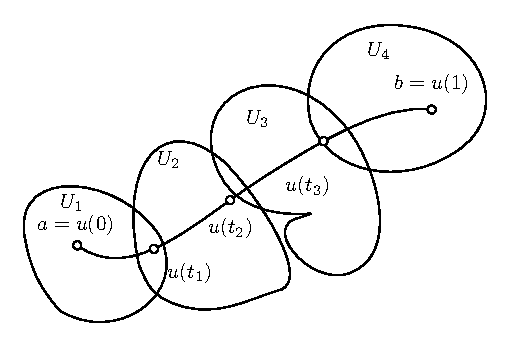
\includegraphics[width=.65\textwidth]{figures/fig05-tikz.pdf}\\图5\end{minipage}\end{center}
对全纯函数层$\OO$作(6.7)的构造，得到$p:|\OO|\to X$。下一引理说明，可借此映射解释沿曲线的解析延拓。
\entry{7.2}{引理}
设$X$为黎曼曲面，$u:[0,1]\to X$从$a$到$b$。则$\psi\in\OO_b$是$\varphi\in\OO_a$沿$u$的解析延拓，当且仅当存在曲线$u$的提升$\widetilde u:[0,1]\to|\OO|$使$\widetilde u(0)=\varphi$、$\widetilde u(1)=\psi$。
\begin{proof}
(a) 若$\psi$为所述延拓，取(7.1)的芽族$\varphi_t$。由$|\OO|$的拓扑定义，$t\mapsto\varphi_t$为连续映射，因而是满足端点条件的提升。

(b) 反之，若存在这样的提升，令$\varphi_t:=\widetilde u(t)$，则$\varphi_t\in\OO_{u(t)}$且端点正确。给定$\tau$，选$\widetilde u(\tau)$的开邻域$[U,f]$。存在$\tau$的邻域$T$使$\widetilde u(T)\subset[U,f]$，故$u(T)\subset U$且$\varphi_t=\rho_{u(t)}(f)$（$t\in T$）。这正是解析延拓的条件。
\end{proof}
由提升唯一性(4.8)，函数芽的解析延拓若存在，就唯一确定。另一个推论是单值性定理。
\entry{7.3}{单值性定理}
设$X$为黎曼曲面，$u_0,u_1:[0,1]\to X$为从$a$到$b$的同伦曲线。设$u_s$（$0\le s\le1$）为从$u_0$到$u_1$的形变，函数芽$\varphi\in\OO_a$可沿每条$u_s$解析延拓。
\sourcepage{46}
则沿$u_0,u_1$所得的函数芽$\psi\in\OO_b$相同。
\begin{proof}
对局部同胚$|\OO|\to X$应用(4.10)；由(6.10)，$|\OO|$为Hausdorff空间。
\end{proof}
\entry{7.4}{推论}
设$X$为单连通黎曼曲面，$a\in X$，$\varphi\in\OO_a$可沿从$a$出发的每条曲线解析延拓。则存在整体定义的全纯函数$f\in\OO(X)$使$\rho_a(f)=\varphi$。

\textbf{注记。}由恒等定理，$f$唯一。
\begin{proof}
对$x\in X$，令$\psi_x\in\OO_x$为$\varphi$沿任一从$a$到$x$的曲线延拓所得芽。由$X$单连通，它不依赖曲线选择。令$f(x):=\psi_x(x)$，则$f$在$X$上全纯且$\rho_a(f)=\varphi$。
\end{proof}
\entry{7.5}{}
一般地，即使函数芽能沿起终点相同的两条曲线延拓，所得终点芽也可能不同。因此，把从给定芽经解析延拓得到的所有芽合在一起，就得到多值函数。下面将精确说明这一情形。

设$X,Y$为黎曼曲面，$\OO_X,\OO_Y$为其全纯函数层，$p:Y\to X$无分歧全纯。由$p$局部双全纯，对每个$y\in Y$诱导同构$p^*:\OO_{X,p(y)}\to\OO_{Y,y}$。以$p_*:\OO_{Y,y}\to\OO_{X,p(y)}$表示其逆。
\entry{7.6}{定义}
设$X$为黎曼曲面，$a\in X$、$\varphi\in\OO_a$。称四元组$(Y,p,f,b)$为$\varphi$的一个\textbf{解析延拓}，如果：
(i)$Y$为黎曼曲面，$p:Y\to X$无分歧全纯；
(ii)$f$为$Y$上的全纯函数；
(iii)$b\in Y$满足$p(b)=a$且$p_*(\rho_b(f))=\varphi$。

若还满足下述泛性质，则称此延拓\textbf{极大}：对$\varphi$的任意其他解析延拓$(Z,q,g,c)$，存在保纤维全纯映射$F:Z\to Y$，使$F(c)=b$且$F^*(f)=g$。
\sourcepage{47}
极大解析延拓在同构意义下唯一。事实上，若$(Y,p,f,b)$、$(Z,q,g,c)$均极大，则还存在保纤维全纯映射$G:Y\to Z$使$G(b)=c$、$G^*(g)=f$。复合$F\circ G$保纤维且固定$b$，由(4.8)等于$\mathrm{id}_Y$。同理$G\circ F=\mathrm{id}_Z$，故$G$双全纯。
\entry{7.7}{引理}
设$(Y,p,f,b)$为$\varphi\in\OO_a$的解析延拓，$v:[0,1]\to Y$从$b$到$y$。则芽$\psi:=p_*(\rho_y(f))\in\OO_{p(y)}$为$\varphi$沿$u:=p\circ v$的解析延拓。
\begin{proof}
令$\varphi_t:=p_*(\rho_{v(t)}(f))\in\OO_{u(t)}$，则$\varphi_0=\varphi$、$\varphi_1=\psi$。给定$t_0$，选$v(t_0)$、$u(t_0)$的开邻域$V,U$使$p|_V:V\to U$双全纯。令$q:U\to V$为逆，$g:=q^*(f|_V)$。则对每个$\eta\in V$，$p_*(\rho_\eta(f))=\rho_{p(\eta)}(g)$。存在$t_0$的邻域$T$使$v(T)\subset V$，故对$t\in T$，$\rho_{u(t)}(g)=p_*(\rho_{v(t)}(f))=\varphi_t$。这证明所述延拓关系。
\end{proof}
\entry{7.8}{定理}
设$X$为黎曼曲面，$a\in X$，$\varphi\in\OO_a$为全纯函数芽。则$\varphi$存在极大解析延拓$(Y,p,f,b)$。
\begin{proof}
令$Y$为$|\OO|$中包含$\varphi$的连通分支，仍以$p$表示$|\OO|\to X$在$Y$上的限制。由(4.6)，局部同胚$p:Y\to X$使$Y$自然成为黎曼曲面，且$p$全纯。每个$\eta\in Y$为$p(\eta)$处的函数芽，定义$f(\eta):=\eta(p(\eta))$。容易看出$f$全纯，且对每个$\eta\in Y$有$p_*(\rho_\eta(f))=\eta$。令$b:=\varphi$，便得一个解析延拓。

为证极大性，取任一其他延拓$(Z,q,g,c)$。对$\zeta\in Z$，令$x:=q(\zeta)$。由(7.7)，芽$q_*(\rho_\zeta(g))\in\OO_x$由$\varphi$沿从$a$到$x$的曲线延拓得到。由(7.2)，$Y$恰由所有如此得到的芽组成。因此存在唯一$\eta\in Y$满足$\eta=q_*(\rho_\zeta(g))$，定义$F(\zeta):=\eta$。容易验证$F$为保纤维全纯映射，$F(c)=b$且$F^*(f)=g$。
\end{proof}
\sourcepage{48}
\textbf{注记。}本节用于全纯函数芽的方法同样可处理亚纯函数芽，只须考虑映射$|\MM|\to X$。目前尚未处理分歧点；下一节将对代数函数这一特殊情形讨论它们。
\subsection*{习题（第7节）}
\entry{7.1}{}
设$p:Y\to X$为黎曼曲面之间的无分歧全纯覆盖，$f:Y\to\C$全纯。令$b\in Y$、$a:=p(b)$、$\varphi:=p_*(\rho_b(f))\in\OO_a$。证明$(Y,p,f,b)$为$\varphi$的极大解析延拓，当且仅当：对任意不同的$b_1,b_2\in p^{-1}(a)$，芽$\varphi_1:=p_*(\rho_{b_1}(f))$、$\varphi_2:=p_*(\rho_{b_2}(f))$不同。
\entry{7.2}{}
设$\varphi\in\OO_a$可沿黎曼曲面$X$中每条从$a$出发的曲线解析延拓，$(Y,p,f,b)$为其极大解析延拓。证明$p:Y\to X$为覆盖映射。

\section{代数函数}
\sourcepage{48}
复分析中最早遇到的多值函数例子之一是平方根$w=\sqrt z$。这是代数函数的特例；所谓代数函数，是满足代数方程$w^n+a_1(z)w^{n-1}+\cdots+a_n(z)=0$的函数$w=w(z)$，其中系数$a_\nu$为给定亚纯函数。本节构造代数函数的黎曼曲面。它们是固有覆盖，叶数等于代数方程的次数。
\entry{8.1}{初等对称函数}
设$\pi:Y\to X$为$n$叶无分歧全纯覆盖，$f\in\MM(Y)$。每个$x\in X$都有开邻域$U$使$\pi^{-1}(U)$为开集$V_1,\ldots,V_n$的不交并，且$\pi|_{V_\nu}:V_\nu\to U$双全纯。令$\tau_\nu:U\to V_\nu$为逆映射，$f_\nu:=\tau_\nu^*f=f\circ\tau_\nu$。对不定元$T$，写
\[
\prod_{\nu=1}^n(T-f_\nu)=T^n+c_1T^{n-1}+\cdots+c_n.
\]
则$c_\nu$是$U$上的亚纯函数，且$c_\nu=(-1)^\nu S_\nu(f_1,\ldots,f_n)$，其中$S_\nu$为$n$个变量的第$\nu$个初等对称函数。
\sourcepage{49}
在另一点的邻域中作同样构造，所得函数在重叠处相同，因而拼成整体亚纯函数$c_1,\ldots,c_n\in\MM(X)$，称为$f$关于覆盖$Y\to X$的初等对称函数。
\entry{8.2}{定理}
设$\pi:Y\to X$为$n$叶分歧全纯覆盖，$A\subset X$为包含$\pi$的所有临界值的闭离散集，$B=\pi^{-1}(A)$。设$f$为$Y\setminus B$上的全纯（亚纯）函数，$c_1,\ldots,c_n\in\OO(X\setminus A)$（相应地属于$\MM(X\setminus A)$）为其初等对称函数。则$f$可全纯（亚纯）延拓到$Y$，当且仅当所有$c_\nu$均可全纯（亚纯）延拓到$X$。

因此，当覆盖有分歧时，$f\in\MM(Y)$的初等对称函数仍可定义。
\begin{proof}
设$a\in A$，$b_1,\ldots,b_m$为其原像。取$a$的相对紧坐标邻域$(U,z)$，满足$z(a)=0$、$U\cap A=\{a\}$。则$V:=\pi^{-1}(U)$是各$b_\mu$的相对紧邻域。

1. 先设$f\in\OO(Y\setminus B)$。
(a) 若$f$可全纯延拓到各$b_\mu$，则它在$V\setminus\{b_1,\ldots,b_m\}$上有界，因而各$c_\nu$在$U\setminus\{a\}$上有界。由可去奇点定理，它们均可全纯延拓到$a$。

(b) 若各$c_\nu$可全纯延拓到$a$，则它们在$U\setminus\{a\}$上有界。这说明$f$在$V\setminus\{b_1,\ldots,b_m\}$上有界，因为若$x=\pi(y)$，则$f(y)^n+c_1(x)f(y)^{n-1}+\cdots+c_n(x)=0$。再次由可去奇点定理，$f$可全纯延拓到各$b_\mu$。

2. 设$f\in\MM(Y\setminus B)$。
(a) 若$f$可亚纯延拓到各$b_\mu$，令$\phi:=\pi^*z\in\OO(V)$，它在各$b_\mu$处为零。因此$k$足够大时$\phi^kf$可全纯延拓到各$b_\mu$。其初等对称函数为$z^{k\nu}c_\nu$，由第一部分可全纯延拓到$a$，故$c_\nu$可亚纯延拓到$a$。

(b) 反之，若各$c_\nu$可亚纯延拓到$a$，则$k$足够大时所有$z^{k\nu}c_\nu$均可全纯延拓到$a$。由第一部分，$\phi^kf$可全纯延拓到各$b_\mu$，故$f$可亚纯延拓到各$b_\mu$。
\end{proof}
\sourcepage{50}
为后面使用，注意此证明未用$Y$连通；因此$Y$为有限多个黎曼曲面的不交并时结论仍成立。

若$\pi:Y\to X$非常值全纯，则对每个$f\in\MM(X)$，$\pi^*f:=f\circ\pi$是$Y$上的亚纯函数。因此$\pi^*:\MM(X)\to\MM(Y)$为域的单同态。
\entry{8.3}{定理}
设$\pi:Y\to X$为$n$叶分歧全纯覆盖，$f\in\MM(Y)$，$c_1,\ldots,c_n$为其初等对称函数。则
\[
f^n+(\pi^*c_1)f^{n-1}+\cdots+(\pi^*c_{n-1})f+\pi^*c_n=0.
\]
域扩张$\pi^*:\MM(X)\to\MM(Y)$为次数$\le n$的代数扩张。此外，若存在$f\in\MM(Y)$及$x\in X$，其原像$y_1,\ldots,y_n$处的函数值$f(y_\nu)$两两不同，则此扩张次数为$n$。

\textbf{注记。}后面(14.13)、(26.6)将看到，最后一个条件总能满足。
\begin{proof}
上述方程直接由初等对称函数的定义得到。令$L:=\MM(Y)$、$K:=\pi^*\MM(X)$。则每个$f\in L$均在$K$上代数，极小多项式次数不超过$n$。选极小多项式次数$n_0$最大的元素$f_0$。断言$L=K(f_0)$。任取$f\in L$，由本原元定理，存在$g\in L$使$K(f_0,f)=K(g)$。由$n_0$的定义，$\dim_KK(g)\le n_0$；另一方面$\dim_KK(f_0,f)\ge\dim_KK(f_0)=n_0$。故$K(f_0)=K(f_0,f)$，$f\in K(f_0)$。

最后，若$f$的极小多项式次数为$m<n$，则$f$在每个$x\in X$上方至多取$m$个不同值，因此若有题述$f,x$，扩张次数必须为$n$。
\end{proof}
\sourcepage{51}
\entry{8.4}{定理}
设$X$为黎曼曲面，$A\subset X$为闭离散集，$X':=X\setminus A$，$Y'$为另一黎曼曲面，$\pi':Y'\to X'$为固有无分歧全纯覆盖。则它可延拓为$X$的分歧覆盖：存在黎曼曲面$Y$、固有全纯映射$\pi:Y\to X$，以及保纤维双全纯映射$\varphi:Y\setminus\pi^{-1}(A)\to Y'$。
\begin{proof}
对各$a\in A$选坐标邻域$(U_a,z_a)$，使$z_a(a)=0$，$z_a(U_a)=D$为单位圆盘，不同$U_a$互不相交。令$U_a^*:=U_a\setminus\{a\}$。由$\pi'$固有，$\pi'^{-1}(U_a^*)$只有有限多个连通分支$V_{a\nu}^*$（$\nu=1,\ldots,n(a)$）。每个$\pi'|_{V_{a\nu}^*}:V_{a\nu}^*\to U_a^*$为无分歧覆盖，设叶数为$k_{a\nu}$。由(5.10)，存在双全纯映射$\zeta_{a\nu}:V_{a\nu}^*\to D^*$，满足$z_a\circ\pi'=\pi_{a\nu}\circ\zeta_{a\nu}$，其中$\pi_{a\nu}(\zeta)=\zeta^{k_{a\nu}}$。

选两两不同且不属于$Y'$的“理想点”$P_{a\nu}$。在$Y:=Y'\cup\{P_{a\nu}:a\in A,\ \nu=1,\ldots,n(a)\}$上恰有一个拓扑满足：若$W_i$为$a$的邻域基，则$\{P_{a\nu}\}\cup(\pi'^{-1}(W_i)\cap V_{a\nu}^*)$为$P_{a\nu}$的邻域基，且在$Y'$上诱导原拓扑。这使$Y$成为Hausdorff空间。定义$\pi|_{Y'}=\pi'$、$\pi(P_{a\nu})=a$，容易验证$\pi$固有。

令$V_{a\nu}:=V_{a\nu}^*\cup\{P_{a\nu}\}$，并定义$\zeta_{a\nu}(P_{a\nu})=0$，把原映射延拓为$\zeta_{a\nu}:V_{a\nu}\to D$。把这些坐标卡加入$Y'$的图册。因原$\zeta_{a\nu}$双全纯，新旧坐标卡全纯相容，于是$Y$成为黎曼曲面，$\pi$全纯。按构造$Y\setminus\pi^{-1}(A)=Y'$，故取$\varphi$为恒等映射即得结论。
\end{proof}
\sourcepage{52}
下面说明此延拓在同构意义下唯一。
\entry{8.5}{定理}
设$\pi:Y\to X$、$\tau:Z\to X$为黎曼曲面之间的固有全纯覆盖，$A\subset X$为闭离散集，令$X':=X\setminus A$、$Y':=\pi^{-1}(X')$、$Z':=\tau^{-1}(X')$。则每个保纤维双全纯映射$\sigma':Y'\to Z'$均可延拓为保纤维双全纯映射$\sigma:Y\to Z$。特别地，每个覆盖变换$\sigma'\in\operatorname{Deck}(Y'/X')$均可延拓为$\sigma\in\operatorname{Deck}(Y/X)$。
\begin{proof}
取$a\in A$的坐标邻域$(U,z)$，$z(a)=0$、$z(U)=D$。令$U^*:=U\setminus\{a\}$，可缩小$U$使$\pi,\tau$在$U^*$上均无分歧。设$V_1,\ldots,V_n$、$W_1,\ldots,W_m$分别为$\pi^{-1}(U)$、$\tau^{-1}(U)$的连通分支。去掉$a$的原像得到$V_\nu^*,W_\mu^*$，它们是相应穿孔原像的连通分支。

由于$\sigma'$在穿孔原像之间双全纯，$n=m$；重新编号可使$\sigma'(V_\nu^*)=W_\nu^*$。由(5.11)，$V_\nu\cap\pi^{-1}(a)$、$W_\nu\cap\tau^{-1}(a)$各恰有一点$b_\nu,c_\nu$。令$b_\nu\mapsto c_\nu$即可把$\sigma'$延拓为两个完整原像之间的双射。由$\pi|_{V_\nu}$、$\tau|_{W_\nu}$固有，延拓为同胚，再由可去奇点定理为双全纯映射；这里由(5.11)，$V_\nu,W_\nu$均同构于圆盘，所以可用该定理。对每个$a\in A$如此处理，便得所需$\sigma$。
\end{proof}
\entry{8.6}{定义}
设$\pi:Y\to X$为分歧全纯覆盖，$A$为临界值集，$X':=X\setminus A$、$Y':=\pi^{-1}(X')$。若$Y'\to X'$为Galois覆盖，则称$Y\to X$为Galois覆盖。定理(8.5)保证此定义与(5.5)相容。
\entry{8.7}{引理}
设$c_1,\ldots,c_n$在$D(R):=\{z:|z|<R\}$（$R>0$）上全纯，$w_0$为多项式$w^n+c_1(0)w^{n-1}+\cdots+c_n(0)$的单零点。
\sourcepage{53}
则存在$0<r\le R$及$D(r)$上的全纯函数$\varphi$，使$\varphi(0)=w_0$且$\varphi^n+c_1\varphi^{n-1}+\cdots+c_n=0$。
\begin{proof}
令$F(z,w):=w^n+c_1(z)w^{n-1}+\cdots+c_n(z)$。存在$\varepsilon>0$使$F(0,\cdot)$在闭圆盘$|w-w_0|\le\varepsilon$内只有单零点$w_0$。由连续性，存在$0<r\le R$使$F$在$|z|<r$、$|w-w_0|=\varepsilon$上无零点。对固定$z\in D(r)$，
\[
n(z):=\frac1{2\pi i}\int_{|w-w_0|=\varepsilon}\frac{F_w(z,w)}{F(z,w)}\,dw
\]
给出$F(z,\cdot)$在圆内的零点数。由$n(0)=1$及连续性，所有$z$均有$n(z)=1$。由留数定理，此唯一零点为
\[
\varphi(z)=\frac1{2\pi i}\int_{|w-w_0|=\varepsilon}w\frac{F_w(z,w)}{F(z,w)}\,dw.
\]
积分全纯依赖$z$，故$\varphi$全纯且$F(z,\varphi(z))=0$。
\end{proof}
\entry{8.8}{推论}
设$\OO_x$为黎曼曲面一点$x$处的全纯函数芽环，$P(T)=T^n+c_1T^{n-1}+\cdots+c_n\in\OO_x[T]$。若$p(T):=T^n+c_1(x)T^{n-1}+\cdots+c_n(x)$有$n$个互异零点$w_1,\ldots,w_n$，则存在$\varphi_\nu\in\OO_x$满足$\varphi_\nu(x)=w_\nu$及$P(T)=\prod_{\nu=1}^n(T-\varphi_\nu)$。
\entry{8.9}{定理}
设$X$为黎曼曲面，$P(T)=T^n+c_1T^{n-1}+\cdots+c_n\in\MM(X)[T]$为$n$次不可约多项式。则存在黎曼曲面$Y$、$n$叶分歧全纯覆盖$\pi:Y\to X$及亚纯函数$F\in\MM(Y)$，使$(\pi^*P)(F)=0$。
\sourcepage{54}
三元组$(Y,\pi,F)$在如下意义下唯一：若$(Z,\tau,G)$有对应性质，则恰有一个保纤维双全纯映射$\sigma:Z\to Y$使$G=\sigma^*F$。

为简化术语，称$(Y,\pi,F)$为多项式$P(T)$定义的\textbf{代数函数}。

\textbf{注记。}经典情形为$X=\PP^1$。由(2.9)，此时系数$c_\nu$为一变量有理函数。由$\PP^1$紧及$\pi$固有，$Y$也紧。
\begin{proof}
令$\Delta\in\MM(X)$为$P$的判别式，即系数的某个多项式。它不恒为零，否则$P$可约。可取闭离散集$A$使在每个$x\in X':=X\setminus A$处，各$c_\nu$全纯且$\Delta(x)\ne0$。故$p_x(T):=T^n+c_1(x)T^{n-1}+\cdots+c_n(x)$有$n$个互异零点。

使用(6.7)的伴随空间$|\OO|\to X$。令$Y'\subset|\OO|$为所有满足$P(\varphi)=0$的芽$\varphi\in\OO_x$（$x\in X'$）之集，$\pi':Y'\to X'$为典范投影。由(8.8)，每个$x$都有开邻域$U\subset X'$及$f_1,\ldots,f_n\in\OO(U)$使$P(T)=\prod_{\nu=1}^n(T-f_\nu)$。于是$\pi'^{-1}(U)=\bigcup_{\nu=1}^n[U,f_\nu]$为不交并，每个$\pi'|_{[U,f_\nu]}$为到$U$的同胚，故$\pi'$为覆盖。$Y'$的连通分支为覆盖$X'$的黎曼曲面。

定义$f:Y'\to\C$，$f(\varphi):=\varphi(\pi'(\varphi))$。则$f$全纯，且对所有$y\in Y'$有$f(y)^n+c_1(\pi'(y))f(y)^{n-1}+\cdots+c_n(\pi'(y))=0$。由(8.4)，覆盖延拓为固有全纯覆盖$\pi:Y\to X$，其中将$Y'$等同于$\pi^{-1}(X')$。由(8.2)，$f$延拓为$F\in\MM(Y)$，且$(\pi^*P)(F)=0$。

须证$Y$连通。否则，它有有限多个连通分支$Y_1,\ldots,Y_k$，每个$\pi|_{Y_i}$为$n_i$叶固有全纯覆盖，$\sum_i n_i=n$。
\sourcepage{55}
利用$F|_{Y_i}$的初等对称函数得到$n_i$次多项式$P_i\in\MM(X)[T]$，使$P=P_1\cdots P_k$，与不可约性矛盾。

唯一性：设$(Z,\tau,G)$为另一个由$P$定义的代数函数。令$B\subset Z$为$G$的极点集与$\tau$的分歧点集之并，$A':=\tau(B)$，并令$X'':=X'\setminus A'$、$Y'':=\pi^{-1}(X'')$、$Z'':=\tau^{-1}(X'')$。对$z\in Z''$、$x=\tau(z)$，利用$\tau$局部双全纯把$G$在$z$处的芽送到$\varphi\in\OO_x$。则$P(\varphi)=0$，由$Y'$的构造，$\varphi$为$x$上的唯一相应点。定义$\sigma''(z):=\varphi$。

按定义$\sigma''$连续且保纤维，因而全纯。又由$\pi|_{Y''}$连续及$\tau|_{Z''}$固有，$\sigma''$固有，从而满射。因为$Y''\to X''$与$Z''\to X''$叶数相同，$\sigma''$双全纯，且$G|_{Z''}=(\sigma'')^*(F|_{Y''})$。由(8.5)，它延拓为保纤维双全纯映射$\sigma:Z\to Y$，满足$G=\sigma^*F$。

若这样的$\sigma$不唯一，则存在非恒等覆盖变换$\alpha:Y\to Y$使$\alpha^*F=F$。但$F$在每个$x\in X'$的纤维上取互异值，因此不可能。唯一性得证。
\end{proof}
\entry{8.10}{例}
设$f(z)=(z-a_1)\cdots(z-a_n)$，各$a_j$互异。把$f$看作$\PP^1$上的亚纯函数。多项式$P(T)=T^2-f$在$\MM(\PP^1)$上不可约，定义通常记为$\sqrt{f(z)}$的代数函数。其黎曼曲面$\pi:Y\to\PP^1$可按上述构造描述。令$A:=\{a_1,\ldots,a_n,\infty\}$、$X':=\PP^1\setminus A$、$Y':=\pi^{-1}(X')$，则$Y'\to X'$为无分歧2叶覆盖。因此，任一满足$\varphi^2=f$的芽$\varphi\in\OO_x$（$x\in X'$）均可沿$X'$内每条曲线延拓。再看例外点的邻域。

(a) 对各$j$选$r_j>0$足够小，使圆盘$U_j:=\{z:|z-a_j|<r_j\}$不含$A$的其他点。
\sourcepage{56}
函数$g(z)=\prod_{k\ne j}(z-a_k)$在单连通$U_j$中无零点，故存在全纯$h$使$h^2=g$，从而$f(z)=(z-a_j)h(z)^2$。设$0<\rho<r_j$、$\theta\in\R$、$\zeta=a_j+\rho e^{i\theta}$。由(8.7)，存在芽$\varphi_\zeta$使$\varphi_\zeta^2=f$且$\varphi_\zeta(\zeta)=\sqrt\rho e^{i\theta/2}h(\zeta)$。沿闭曲线$\zeta=a_j+\rho e^{i\theta}$、$0\le\theta\le2\pi$延拓，得到原芽的负值。令$U_j^*=U_j\setminus\{a_j\}$、$V_j^*=\pi^{-1}(U_j^*)$。则$V_j^*\to U_j^*$为(5.10.ii)中$k=2$的连通2叶覆盖；否则它分裂为两个单叶覆盖，沿该闭曲线延拓必返回原芽。因此$Y$在$a_j$之上恰有一点。

(b) 取$r>\max_j|a_j|$，令$U^*:=\{z\in\C:|z|>r\}$、$U:=U^*\cup\{\infty\}$。则$U$同构于圆盘，除$\infty$外不含$A$中点。在$U$上可写$f=z^nF$，其中$F$全纯且无零点。
(i) 若$n$奇，则存在$U$上的亚纯函数$h$使$f(z)=zh(z)^2$；
(ii) 若$n$偶，则存在亚纯$h$使$f(z)=h(z)^2$。
令$V^*:=\pi^{-1}(U^*)$。与(a)同样，(i)时$V^*\to U^*$为连通2叶覆盖，故$Y$在$\infty$上恰有一点；(ii)时分裂为两个单叶覆盖，故$Y$在$\infty$上有两点。
\entry{8.11}{}
若$\pi:Y\to X$为分歧全纯覆盖，则$\operatorname{Deck}(Y/X)$在域$\MM(Y)$的自同构群中有如下表示：对覆盖变换$\sigma$，定义$\sigma f:=f\circ\sigma^{-1}$。显然$f\mapsto\sigma f$为域自同构，且
\[
(\sigma\tau)f=f\circ\tau^{-1}\circ\sigma^{-1}=\sigma(\tau f),
\]
故$\operatorname{Deck}(Y/X)\to\operatorname{Aut}(\MM(Y))$为群同态。
\sourcepage{57}
每个此类自同构都固定子域$\pi^*\MM(X)$中的函数，因此属于Galois群
\[\operatorname{Aut}(\MM(Y)/\pi^*\MM(X)).\]
\entry{8.12}{定理}
设$K:=\MM(X)$，$P\in K[T]$为$n$次首一不可约多项式，$(Y,\pi,F)$为其定义的代数函数，$L:=\MM(Y)$。借助$\pi^*$把$K$视为$L$的子域，则$L:K$为$n$次扩张，且$L\cong K[T]/(P)$。覆盖变换$\sigma$诱导固定$K$的域自同构$f\mapsto\sigma f=f\circ\sigma^{-1}$，所定义的映射$\operatorname{Deck}(Y/X)\to\operatorname{Aut}(L/K)$为群同构。覆盖为Galois覆盖，当且仅当域扩张$L:K$为Galois扩张。
\begin{proof}
扩张次数为$n$由(8.3)末句得到。由$P(F)=0$有同态$K[T]/(P)\to L$，两域在$K$上次数均为$n$，故为同构。

群映射单射，因为非恒等覆盖变换$\sigma$满足$\sigma F\ne F$。为证满射，取$\alpha\in\operatorname{Aut}(L/K)$，则$(Y,\pi,\alpha F)$也为$P$定义的代数函数。由(8.9)唯一性，存在覆盖变换$\tau$使$\alpha F=\tau^*F$。令$\sigma:=\tau^{-1}$，则$\sigma F=F\circ\sigma^{-1}=F\circ\tau=\alpha F$。由于$L=K(F)$，$f\mapsto\sigma f$即为$\alpha$。

最后，$Y/X$为Galois覆盖当且仅当覆盖变换群有$n$个元素；$L/K$为Galois扩张当且仅当自同构群有$n$个元素。因此最后断言成立。
\end{proof}
\entry{8.13}{Puiseux展开}
以$\C\{\{z\}\}$表示在某穿孔圆盘$0<|z|<r$内收敛、主部有限的Laurent级数$\varphi(z)=\sum_{\nu=k}^\infty c_\nu z^\nu$所成的域，$r>0$可随元素而异。它同构于复平面上亚纯函数层在0处的茎$\MM_0$，也是$\C\{z\}$的分式域。

考虑$\C\{\{z\}\}$上的$n$次不可约多项式$F(z,w)=w^n+a_1(z)w^{n-1}+\cdots+a_n(z)$。
\sourcepage{58}
对某$r>0$，各$a_\nu$均为$D(r)$上的亚纯函数，故$F\in\MM(D(r))[w]$，且显然在此域上仍不可约。取$r$足够小，使每个$a\in D(r)\setminus\{0\}$处$F(a,w)$均无重根。令$(Y,\pi,f)$为(8.9)意义下$F$定义的代数函数。则$\pi:Y\to D(r)$是仅可能在原点上方分歧的$n$叶固有全纯映射。由(5.11)，存在同构$\alpha:D(\rho)\to Y$，$\rho=\sqrt[n]r$，满足$\pi(\alpha(\zeta))=\zeta^n$。由$F(\pi,f)=0$得$F(\zeta^n,\varphi(\zeta))=0$，其中$\varphi:=f\circ\alpha$。这证明了下一定理。
\entry{8.14}{定理（Puiseux）}
设$F(z,w)=w^n+a_1(z)w^{n-1}+\cdots+a_n(z)\in\C\{\{z\}\}[w]$为$n$次不可约多项式。则存在Laurent级数$\varphi(\zeta)=\sum_{\nu=k}^\infty c_\nu\zeta^\nu\in\C\{\{\zeta\}\}$，使$F(\zeta^n,\varphi(\zeta))=0$在$\C\{\{\zeta\}\}$中成立。

\textbf{注记。}
(1) 若各系数$a_\nu$全纯，即属于$\C\{z\}$，则$\varphi\in\C\{\zeta\}$。因为此时(8.13)的$f$在$Y$上全纯。

(2) 定理也可表述为方程$F(z,w)=0$可由Puiseux级数
\sourcepage{59}
\[
w=\varphi(\sqrt[n]z)=\sum_{\nu=k}^\infty c_\nu z^{\nu/n}
\]
求解。

(3) 代数解释如下：通过映射$\C\{\{z\}\}\to\C\{\{\zeta\}\}$、$z\mapsto\zeta^n$，后者成为前者的$n$次扩张，以$1,\zeta,\ldots,\zeta^{n-1}$为基。级数$\varphi(\zeta)$为$F$在此扩张中的一个根。令$\varepsilon$为$n$次本原单位根，例如$e^{2\pi i/n}$。对$k=0,\ldots,n-1$有$(\varepsilon^k\zeta)^n=\zeta^n$，故$F(\zeta^n,\varphi(\varepsilon^k\zeta))=0$。这些级数互异，因而$\C\{\{\zeta\}\}$为$F$的分裂域。
\subsection*{习题（第8节）}
\entry{8.1}{}
设$X,Y$为紧黎曼曲面，且$\MM(X),\MM(Y)$作为$\C$代数同构。证明$X,Y$同构。［提示：把$X,Y$表示为同一个不可约多项式$P\in\MM(\PP^1)[T]$所定义的代数函数的黎曼曲面。还可利用推论(14.13)将证明的事实：紧黎曼曲面上的亚纯函数分离点。］
\entry{8.2}{}
设$X,Y$为紧黎曼曲面，$a_1,\ldots,a_n\in X$、$b_1,\ldots,b_m\in Y$，$X':=X\setminus\{a_1,\ldots,a_n\}$、$Y':=Y\setminus\{b_1,\ldots,b_m\}$。证明每个同构$f:X'\to Y'$均可延拓为同构$\widetilde f:X\to Y$。
\entry{8.3}{}
令$F(z,w):=w^2-z^3w+z\in\C\{\{z\}\}[w]$。
(a)证明$F$在$\C\{\{z\}\}$上不可约。
(b)求由$F(z,w)=0$定义的代数函数的Puiseux展开$w=\sum_{\nu=0}^\infty c_\nu z^{\nu/2}$。

\section{微分形式}
\sourcepage{59--60}
本节引入黎曼曲面上的微分形式。除全纯和亚纯形式外，考虑仅在实意义下可微的形式也很重要。
\entry{9.1}{}
设$U\subset\C$开。写$z=x+iy$，以实坐标$x,y$将$\C$等同于$\R^2$。用$\mathcal E(U)$表示关于$x,y$无限次可微的函数$f:U\to\C$构成的$\C$代数。除$\partial/\partial x,\partial/\partial y$外，还考虑
\[
\frac\partial{\partial z}:=\frac12\left(\frac\partial{\partial x}-i\frac\partial{\partial y}\right),\qquad
\frac\partial{\partial\bar z}:=\frac12\left(\frac\partial{\partial x}+i\frac\partial{\partial y}\right).
\]
Cauchy--Riemann方程表明，全纯函数空间$\OO(U)$是$\partial/\partial\bar z:\mathcal E(U)\to\mathcal E(U)$的核。
\entry{9.2}{}
利用复坐标卡，可以在任意黎曼曲面$X$上定义可微函数。对开集$Y\subset X$，令$\mathcal E(Y)$为所有函数$f:Y\to\C$之集，满足：对每个$U\subset Y$上的坐标卡$z:U\to V$，存在$\widetilde f\in\mathcal E(V)$使$f|_U=\widetilde f\circ z$。显然$\widetilde f=f\circ\psi$唯一，其中$\psi=z^{-1}$。配自然限制映射得到可微函数层$\mathcal E$。下文“可微”总指无限次可微。

在坐标邻域$(U,z)$中写$z=x+iy$，可按显然方式定义$\partial/\partial x$、$\partial/\partial y$、$\partial/\partial z$、$\partial/\partial\bar z$。

对$a\in X$，茎$\mathcal E_a$由$a$处的可微函数芽组成。以$\mathfrak m_a\subset\mathcal E_a$表示在$a$处为零的芽构成的向量子空间，$\mathfrak m_a^2$表示其中二阶消失的芽所成子空间。所谓二阶消失，是指可由函数$f$代表，使在$a$的某坐标邻域中$\partial f/\partial x(a)=\partial f/\partial y(a)=0$。这一定义与局部坐标的选择无关。
\entry{9.3}{定义}
商向量空间$T_a^{(1)}:=\mathfrak m_a/\mathfrak m_a^2$称为$X$在$a$处的\textbf{余切空间}（cotangent space）。
\sourcepage{61}
若$U$是$a$的开邻域，$f\in\mathcal E(U)$，则$f$在$a$处的\textbf{微分}为$d_af:=(f-f(a))\bmod\mathfrak m_a^2\in T_a^{(1)}$。函数$f-f(a)$在$a$处为零，故代表$\mathfrak m_a$的元素，其等价类即$d_af$。
\entry{9.4}{定理}
设$(U,z)$为$a\in X$的坐标邻域，$z=x+iy$。则$d_ax,d_ay$为$T_a^{(1)}$的一组基，$d_az,d_a\bar z$也为一组基。若$f$在$a$附近可微，则
\[
d_af=\frac{\partial f}{\partial x}(a)d_ax+\frac{\partial f}{\partial y}(a)d_ay
=\frac{\partial f}{\partial z}(a)d_az+\frac{\partial f}{\partial\bar z}(a)d_a\bar z.
\]
\begin{proof}
(a) 对$t\in T_a^{(1)}$取代表元$\varphi\in\mathfrak m_a$。在$a$处作Taylor展开，$\varphi=c_1(x-x(a))+c_2(y-y(a))+\psi$，其中$\psi\in\mathfrak m_a^2$。取等价类得$t=c_1d_ax+c_2d_ay$。

(b) 若$c_1d_ax+c_2d_ay=0$，则$c_1(x-x(a))+c_2(y-y(a))\in\mathfrak m_a^2$。分别对$x,y$求偏导，得$c_1=c_2=0$，故线性无关。

(c) $f-f(a)=f_x(a)(x-x(a))+f_y(a)(y-y(a))+g$，其中$g$二阶消失，故取商即得第一式。关于$d_az,d_a\bar z$的结论可同样证明。
\end{proof}
\sourcepage{62}
\entry{9.5}{型为$(1,0)$与$(0,1)$的余切向量}
若$(U,z),(U',z')$均为$a$的坐标邻域，则$\partial z'/\partial z(a)=:c\in\C^*$，$\partial\bar z'/\partial\bar z(a)=\bar c$，而$\partial z'/\partial\bar z(a)=\partial\bar z'/\partial z(a)=0$。故$d_az'=c\,d_az$、$d_a\bar z'=\bar c\,d_a\bar z$。因此$d_az$与$d_a\bar z$各自张成的一维子空间与坐标选择无关。记
\[
T_a^{1,0}:=\C d_az,\quad T_a^{0,1}:=\C d_a\bar z,\quad T_a^{(1)}=T_a^{1,0}\oplus T_a^{0,1}.
\]
相应元素称为$(1,0)$型、$(0,1)$型余切向量。按此直和分解定义$d_af=d'_af+d''_af$，其中
\[
d'_af=\frac{\partial f}{\partial z}(a)d_az,\qquad d''_af=\frac{\partial f}{\partial\bar z}(a)d_a\bar z.
\]
\entry{9.6}{定义}
开集$Y\subset X$上的\textbf{一次微分形式}或\textbf{1形式}是指映射$\omega:Y\to\coprod_{a\in Y}T_a^{(1)}$，满足$\omega(a)\in T_a^{(1)}$。若每个$a$均有$\omega(a)\in T_a^{1,0}$（相应地$T_a^{0,1}$），则称$\omega$为$(1,0)$型（$(0,1)$型）。
\entry{9.7}{例}
(a) 对$f\in\mathcal E(Y)$，由$(df)(a):=d_af$、$(d'f)(a):=d'_af$、$(d''f)(a):=d''_af$定义的映射均为1形式。显然$f$全纯当且仅当$d''f=0$。

(b) 若$\omega$为1形式，$f:Y\to\C$为函数，则$(f\omega)(a):=f(a)\omega(a)$也为1形式。

\textbf{注记。}在坐标卡$(U,z)$中，写$z=x+iy$，每个1形式均可写为$\omega=f\,dx+g\,dy=\varphi\,dz+\psi\,d\bar z$。
\sourcepage{63}
一般而言，系数函数甚至不必连续。
\entry{9.8}{定义}
称$Y$上的1形式$\omega$\textbf{可微}，若对每个坐标卡$(U,z)$，在$U\cap Y$上可写$\omega=f\,dz+g\,d\bar z$，其中$f,g\in\mathcal E(U\cap Y)$；称其\textbf{全纯}，若可写$\omega=f\,dz$，$f\in\OO(U\cap Y)$。

\textbf{记号。}以$\mathcal E^{(1)}(U)$表示可微1形式空间，以$\mathcal E^{1,0}(U),\mathcal E^{0,1}(U)$表示其中相应型的子空间，以$\Omega(U)$表示全纯1形式空间。配自然限制映射，它们均为$X$上的向量空间层。
\entry{9.9}{留数}
设$\omega$在$Y\setminus\{a\}$上为全纯1形式。取坐标邻域$(U,z)$使$U\subset Y$、$z(a)=0$，在$U\setminus\{a\}$上写$\omega=f\,dz$，并作Laurent展开$f=\sum_{n=-\infty}^\infty c_nz^n$。若所有$n<0$时$c_n=0$，则$\omega$可全纯延拓到$a$，称$a$为可去奇点。若存在$k<0$使$c_k\ne0$，且所有$n<k$时$c_n=0$，则原文称$\omega$在$a$有$k$阶极点。\translatornote{这里原文把阶数写为负数$k$；通常称极点阶数为$-k>0$。}若有无限多个$n<0$使$c_n\ne0$，则$a$为本性奇点。

系数$c_{-1}$称为$\omega$在$a$处的\textbf{留数}，记为$\operatorname{Res}_a\omega:=c_{-1}$。

\textbf{引理。}留数与坐标卡的选择无关。
\begin{proof}
设$V$为$a$的开邻域。

断言(a)：若$g$在$V\setminus\{a\}$上全纯，则$dg$在$a$处留数为零，与坐标无关。
\sourcepage{64}
在任意$z(a)=0$的坐标中展开$g=\sum_{n=-\infty}^\infty c_nz^n$，则$dg=\sum_n nc_nz^{n-1}\,dz$，故$z^{-1}\,dz$的系数为零。

断言(b)：若$\phi$在$V$上全纯并在$a$有一阶零点，则$\operatorname{Res}_a(\phi^{-1}d\phi)=1$，与坐标无关。事实上，在任意$z(a)=0$的坐标中，$\phi=zh$，$h$在$a$全纯且非零。于是$d\phi=h\,dz+z\,dh$，故$d\phi/\phi=dz/z+dh/h$。最后一项在$a$全纯，所以留数为1。

现在写$\omega=f\,dz$，$f=\sum_n c_nz^n$，并令
\[
g:=\sum_{n=-\infty}^{-2}\frac{c_n}{n+1}z^{n+1}+\sum_{n=0}^\infty\frac{c_n}{n+1}z^{n+1}.
\]
则$\omega=dg+c_{-1}z^{-1}dz$。由(a)、(b)，其留数为$c_{-1}$，与坐标无关。
\end{proof}
\entry{9.10}{亚纯微分形式}
若存在开集$Y'\subset Y$，使$\omega$在$Y'$上为全纯1形式，$Y\setminus Y'$仅含孤立点，且在其中每点均有极点，则称$\omega$为$Y$上的\textbf{亚纯微分形式}。
\sourcepage{65}
以$\MM^{(1)}(Y)$表示全体亚纯1形式。配自然代数运算和通常限制映射，它们构成向量空间层。$X$上的亚纯1形式也称\textbf{阿贝尔微分}。处处全纯的称为第一类；在每个极点处留数均为零的称为第二类；其余称为第三类。
\entry{9.11}{外积}
为定义2形式，回顾向量空间的外积。若$V$为复向量空间，则$\Lambda^2V$的元素是形如$v_1\wedge v_2$的元素的有限和，并满足
\begin{gather*}
v_1\wedge v_2=-v_2\wedge v_1,\qquad
(v_1+v_2)\wedge v_3=v_1\wedge v_3+v_2\wedge v_3,\\
(\lambda v_1)\wedge v_2=\lambda(v_1\wedge v_2)=v_1\wedge(\lambda v_2).
\end{gather*}
若$(e_1,\ldots,e_n)$为$V$的基，则$e_i\wedge e_j$（$i<j$）构成$\Lambda^2V$的基。这些性质完全刻画$\Lambda^2V$。

对余切空间令$T_a^{(2)}:=\Lambda^2T_a^{(1)}$。在坐标$z=x+iy$中，$d_ax\wedge d_ay$为其基，$d_az\wedge d_a\bar z=-2i\,d_ax\wedge d_ay$为另一组基。因此$\dim T_a^{(2)}=1$。
\entry{9.12}{定义}
$Y$上的\textbf{2形式}是映射$\omega:Y\to\coprod_{a\in Y}T_a^{(2)}$，满足$\omega(a)\in T_a^{(2)}$。若在每张坐标卡中可写$\omega=f\,dz\wedge d\bar z$，$f\in\mathcal E(U\cap Y)$，则称其可微。此表达式意指$\omega(a)=f(a)d_az\wedge d_a\bar z$。以$\mathcal E^{(2)}(Y)$表示可微2形式空间。

\textbf{例。}若$\omega_1,\omega_2\in\mathcal E^{(1)}(Y)$，定义$(\omega_1\wedge\omega_2)(a):=\omega_1(a)\wedge\omega_2(a)$便得2形式。若$f\in\mathcal E(Y)$、$\omega\in\mathcal E^{(2)}(Y)$，则$(f\omega)(a):=f(a)\omega(a)$也为2形式。
\sourcepage{66}
\entry{9.13}{形式的外微分}
现在定义$d,d',d'':\mathcal E^{(1)}(U)\to\mathcal E^{(2)}(U)$。局部地，可微1形式可写为有限和$\omega=\sum_k f_k\,dg_k$，其中$f_k,g_k$可微，例如$\omega=f_1dz+f_2d\bar z$。令
\[
d\omega:=\sum_k df_k\wedge dg_k,\qquad d'\omega:=\sum_k d'f_k\wedge dg_k,\qquad d''\omega:=\sum_k d''f_k\wedge dg_k.
\]
\translatornote{以上$d',d''$的公式照录原文。若允许任意可微$g_k$，它们一般依赖表示：例如$d(z\bar z)=\bar z\,dz+z\,d\bar z$，两种表示给出的$d'$不同。通常应按形式的型定义$\partial,\bar\partial$；在坐标表达式$\omega=f\,dz+g\,d\bar z$中，取$d'\omega=g_z\,dz\wedge d\bar z$、$d''\omega=-f_{\bar z}\,dz\wedge d\bar z$。下文其余公式按此通常定义理解。}
现在须证明定义不依赖表示。对$d$证明如下，原文称其他情形类似。

若$\omega=\sum_k f_kdg_k=\sum_j\widetilde f_jd\widetilde g_j$，取坐标$z=x+iy$。由$dg_k=(g_k)_x dx+(g_k)_y dy$及对应的另一表达式，得
\[
\sum_k f_k(g_k)_x=\sum_j\widetilde f_j(\widetilde g_j)_x,\qquad
\sum_k f_k(g_k)_y=\sum_j\widetilde f_j(\widetilde g_j)_y.
\]
分别取适当偏导再相减，混合二阶导数抵消，得
\[
\sum_k((f_k)_y(g_k)_x-(f_k)_x(g_k)_y)
=\sum_j((\widetilde f_j)_y(\widetilde g_j)_x-(\widetilde f_j)_x(\widetilde g_j)_y).
\]
另一方面，$\sum_kdf_k\wedge dg_k=\sum_k((f_k)_x(g_k)_y-(f_k)_y(g_k)_x)dx\wedge dy$，另一表示亦然，故两者相等。
\entry{9.14}{初等性质}
对$f\in\mathcal E(U)$、$\omega\in\mathcal E^{(1)}(U)$，有
\begin{enumerate}[label=(\roman*)]
\item $ddf=d'd'f=d''d''f=0$；
\item $d\omega=d'\omega+d''\omega$；
\item $d(f\omega)=df\wedge\omega+f\,d\omega$，$d',d''$有类似规则。
\end{enumerate}
这些规则直接由定义得到，例如$ddf=d(1\cdot df)=d1\wedge df=0$。
\sourcepage{67}
由(i)、(ii)得$d'd''f=-d''d'f$，因为$0=(d'+d'')(d'+d'')f=d'd''f+d''d'f$。在坐标$z=x+iy$中，
\[
d'd''f=\frac{\partial^2 f}{\partial z\partial\bar z}dz\wedge d\bar z
=\frac1{2i}\left(\frac{\partial^2f}{\partial x^2}+\frac{\partial^2f}{\partial y^2}\right)dx\wedge dy.
\]
因此，称黎曼曲面开集上的可微函数$f$\textbf{调和}，如果$d'd''f=0$。
\entry{9.15}{定义}
若可微1形式$\omega$满足$d\omega=0$，称其\textbf{闭}（closed）；若存在$f\in\mathcal E(Y)$使$\omega=df$，称其\textbf{恰当}（exact）。

\textbf{注记。}由$ddf=0$，恰当形式均闭。反之一般不成立，下一节进一步研究此问题。
\entry{9.16}{定理}
(a) 每个全纯1形式$\omega\in\Omega(Y)$均闭。
(b) 每个闭的$(1,0)$型1形式$\omega\in\mathcal E^{1,0}(Y)$均全纯。
\begin{proof}
局部写$\omega=f\,dz$，则
\[
d\omega=df\wedge dz=(f_zdz+f_{\bar z}d\bar z)\wedge dz=-f_{\bar z}dz\wedge d\bar z.
\]
故$d\omega=0$等价于$f_{\bar z}=0$，两项结论随即得到。
\end{proof}
\textbf{推论。}若$u$调和，则$d'u$为全纯1形式，因为$dd'u=d''d'u=0$。
\entry{9.17}{微分形式的拉回}
设$F:X\to Y$为全纯映射。对开集$U\subset Y$，$F$诱导$F^*:\mathcal E(U)\to\mathcal E(F^{-1}(U))$，$F^*f=f\circ F$。类似地定义$F^*:\mathcal E^{(k)}(U)\to\mathcal E^{(k)}(F^{-1}(U))$（$k=1,2$）。
\sourcepage{68}
局部把形式写为$\sum_j f_jdg_j$或$\sum_j f_jdg_j\wedge dh_j$，定义
\begin{gather*}
F^*\left(\sum_jf_jdg_j\right):=\sum_j(F^*f_j)d(F^*g_j),\\
F^*\left(\sum_jf_jdg_j\wedge dh_j\right):=\sum_j(F^*f_j)d(F^*g_j)\wedge d(F^*h_j).
\end{gather*}
容易验证，这不依赖局部表示，故可拼成唯一的整体向量空间同态。并有
\begin{gather*}
F^*(df)=d(F^*f),\quad F^*(d\omega)=d(F^*\omega),\\
F^*(d'f)=d'(F^*f),\quad F^*(d'\omega)=d'(F^*\omega),
\end{gather*}
$d''$亦有对应公式。

\textbf{推论。}若$f$调和，则$F^*f=f\circ F$也调和，因为$d'd''(F^*f)=d'(F^*d''f)=F^*(d'd''f)=0$。
\subsection*{习题（第9节）}
\entry{9.1}{}
设$p=\exp:\C\to\C^*$为万有覆盖，$\omega=dz/z$为$\C^*$上的全纯1形式。求$p^*\omega$。
\entry{9.2}{}
证明$\C\setminus\{\pm i\}$上的全纯1形式$dz/(1+z^2)$可延拓为$\PP^1\setminus\{\pm i\}$上的全纯1形式$\omega$。令$p=\tan:\C\to\PP^1\setminus\{\pm i\}$（参见习题4.4），求$p^*\omega$。
\entry{9.3}{}
设$p:Y\to X$为黎曼曲面间的全纯映射，$a\in X$、$b\in p^{-1}(a)$，$k$为$p$在$b$处的重数。对$X\setminus\{a\}$上的任意全纯1形式$\omega$，证明$\operatorname{Res}_b(p^*\omega)=k\operatorname{Res}_a\omega$。

\section{微分形式的积分}
\sourcepage{68--69}
微分1形式可沿曲线积分。若形式闭，则积分仅依赖曲线的同伦类。因此在单连通曲面$X$上，对闭1形式沿起点固定、终点变化的曲线作不定积分，得到$X$上的良定义函数。一般地，闭形式的积分产生多值函数，但其多值性质很特殊，本节将详细研究。我们还考虑2形式的积分，以把线积分转为面积分，并证明留数定理。
\subsection*{A. 微分1形式}
\entry{10.1}{}
设$X$为黎曼曲面，$\omega\in\mathcal E^{(1)}(X)$。设$c:[0,1]\to X$为分段连续可微曲线，即存在分割$0=t_0<\cdots<t_n=1$及坐标卡$(U_k,z_k)$，$z_k=x_k+iy_k$，使$c([t_{k-1},t_k])\subset U_k$，且$x_k\circ c,y_k\circ c$在各子区间上有连续一阶导数。在$U_k$上写$\omega=f_kdx_k+g_kdy_k$，定义
\[
\int_c\omega:=\sum_{k=1}^n\int_{t_{k-1}}^{t_k}
\left(f_k(c(t))\frac{d(x_k\circ c)}{dt}+g_k(c(t))\frac{d(y_k\circ c)}{dt}\right)dt.
\]
容易验证，此定义不依赖分割及坐标卡的选择。
\entry{10.2}{定理}
若$c$分段连续可微，$F\in\mathcal E(X)$，则$\int_c dF=F(c(1))-F(c(0))$。
\begin{proof}
取上述分割与坐标卡。在$U_k$上$dF=F_{x_k}dx_k+F_{y_k}dy_k$，所以
\sourcepage{70}
\begin{align*}
\int_c dF&=\sum_k\int_{t_{k-1}}^{t_k}\left(F_{x_k}(c(t))(x_k\circ c)'(t)+F_{y_k}(c(t))(y_k\circ c)'(t)\right)dt\\
&=\sum_k\int_{t_{k-1}}^{t_k}\frac d{dt}F(c(t))dt
=\sum_k(F(c(t_k))-F(c(t_{k-1})))\\&=F(c(1))-F(c(0)).
\end{align*}
\end{proof}
\entry{10.3}{定义}
若$F\in\mathcal E(X)$满足$dF=\omega$，则称$F$为$\omega$的\textbf{原函数}（primitive）。由(9.15)，有原函数的形式必闭。原函数不唯一：若$F$为原函数，则$F+c$也为原函数。反之，两个原函数只差常数，因为$dF=0$由(10.2)可推出$F$为常数。

由(10.2)，已知原函数便可计算线积分，且恰当微分形式沿曲线的积分只依赖起点、终点。
\entry{10.4}{原函数的局部存在性}
设$U:=\{z:|z|<r\}$，$r>0$，$\omega=f\,dx+g\,dy\in\mathcal E^{(1)}(U)$，并假设$d\omega=0$。由$d\omega=(g_x-f_y)dx\wedge dy$，此条件等价于$g_x=f_y$。我们证明其原函数可取为
\[
F(x,y):=\int_0^1(f(tx,ty)x+g(tx,ty)y)\,dt.
\]
它显然无限次可微，只须验证$F_x=f$、$F_y=g$。积分号下求导得
\[
F_x(x,y)=\int_0^1(tf_x(tx,ty)x+tg_x(tx,ty)y+f(tx,ty))\,dt.
\]
\sourcepage{71}
由$g_x=f_y$及$\frac d{dt}f(tx,ty)=f_x(tx,ty)x+f_y(tx,ty)y$，有
\[
F_x=\int_0^1\left(t\frac d{dt}f(tx,ty)+f(tx,ty)\right)dt
=\int_0^1\frac d{dt}(tf(tx,ty))dt=f(x,y).
\]
同理$F_y=g$，故$dF=\omega$。

若$\omega$全纯，证明更简单：写$\omega=f\,dz$，$f(z)=\sum_{n=0}^\infty c_nz^n$，定义$F(z):=\sum_{n=0}^\infty\frac{c_n}{n+1}z^{n+1}$便得全纯原函数。

整体而言，闭形式的原函数通常仅作为多值函数存在。下一定理使此说法精确化。
\entry{10.5}{定理}
设$\omega\in\mathcal E^{(1)}(X)$闭。则存在连通覆盖$p:\widehat X\to X$及$p^*\omega$的原函数$F\in\mathcal E(\widehat X)$。
\begin{proof}
令$\mathcal F$为$\omega$的原函数层：$\mathcal F(U):=\{f\in\mathcal E(U):df=\omega|_U\}$。由于连通区域上两个原函数只差常数，$\mathcal F$满足恒等定理。由(6.10)，伴随空间$|\mathcal F|$为Hausdorff空间。由(10.4)，每个$a\in X$有连通开邻域$U$及原函数$f$。$f+c$（$c\in\C$）恰为$U$上的所有原函数，因此
\[
p^{-1}(U)=\bigcup_{c\in\C}[U,f+c].
\]
\sourcepage{72}
这些集合两两不交，且投影限制均为到$U$的同胚，故$p:|\mathcal F|\to X$为覆盖。取其任意连通分支$\widehat X$，限制仍为覆盖。$\widehat X$由函数芽组成，故自然定义$F(\varphi):=\varphi(p(\varphi))$，直接由定义可知$dF=p^*\omega$。
\end{proof}
\entry{10.6}{推论}
设$\pi:\widetilde X\to X$为万有覆盖，$\omega$为闭1形式。则$\pi^*\omega$有原函数$f\in\mathcal E(\widetilde X)$。
\begin{proof}
取(10.5)的$p:\widehat X\to X$及原函数$F$。由万有性，存在保纤维全纯映射$\tau:\widetilde X\to\widehat X$。令$f:=\tau^*F$，便是$\tau^*(p^*\omega)=\pi^*\omega$的原函数。
\end{proof}
\entry{10.7}{推论}
单连通黎曼曲面上的每个闭1形式都有原函数。

由(10.6)及$\mathrm{id}:X\to X$为万有覆盖即得。
\entry{10.8}{定理}
设$p:\widetilde X\to X$为万有覆盖，$F$为$p^*\omega$的原函数。若$c:[0,1]\to X$分段连续可微，$\widetilde c$为其提升，则$\int_c\omega=F(\widetilde c(1))-F(\widetilde c(0))$。
\begin{proof}
由定义，对任意分段连续可微曲线$v$有$\int_vp^*\omega=\int_{p\circ v}\omega$，再用(10.2)即得。
\end{proof}
\entry{10.9}{注记}
现在可用(10.8)的公式定义闭形式沿任意连续曲线$c$的积分。它不依赖原函数的选择，因为两个原函数只差常数。它也不依赖提升的选择：若$u,v$为$c$的两个提升，由万有覆盖为Galois覆盖，存在覆盖变换$\sigma$使$v=\sigma\circ u$。
\sourcepage{73}
由$p\circ\sigma=p$，$\sigma^*F$也是$p^*\omega$的原函数，故$\sigma^*F-F$为常数。因此
\[
F(v(1))-F(v(0))=\sigma^*F(u(1))-\sigma^*F(u(0))=F(u(1))-F(u(0)).
\]
\entry{10.10}{定理}
设$\omega$为闭1形式。
(a) 若$u,v$为从$a$到$b$的同伦曲线，则$\int_u\omega=\int_v\omega$；
(b) 若$u,v$为自由同伦的闭曲线，则也有此等式。
\begin{proof}
(a) 在万有覆盖中取同起点的提升$\widetilde u,\widetilde v$。由(4.10)，终点亦同，由(10.8)即得。

(b) 若$u,v$的基点分别为$x_0,x_1$，由(3.13)存在从$x_0$到$x_1$的曲线$w$使$u\sim w\cdot v\cdot w^-$。由(a)，
\[
\int_u\omega=\int_{w\cdot v\cdot w^-}\omega=\int_w\omega+\int_v\omega-\int_w\omega=\int_v\omega.
\]
\end{proof}
\entry{10.11}{周期}
由(10.10)，对$\sigma\in\pi_1(X)$可以取任意代表曲线$u$定义$a_\sigma:=\int_\sigma\omega:=\int_u\omega$。这些积分称为$\omega$的\textbf{周期}（period）。显然$\int_{\sigma\tau}\omega=\int_\sigma\omega+\int_\tau\omega$，因而得到群同态$\pi_1(X)\to(\C,+)$，称为$\omega$的\textbf{周期同态}。
\sourcepage{74}
\textbf{例。}$X=\C^*$时，$\pi_1(X)\cong\Z$由$u(t)=e^{2\pi it}$的类生成。对$\omega=dz/z$有$\int_u\omega=2\pi i$，故周期同态为$\Z\to\C$，$n\mapsto2\pi in$；这里同构$\Z\to\pi_1(\C^*)$取$n\mapsto\operatorname{cl}(u^n)$。
\entry{10.12}{自守加项}
设$p:\widetilde X\to X$为万有覆盖，$G:=\operatorname{Deck}(\widetilde X/X)\cong\pi_1(X)$。对$\sigma\in G$及函数$f:\widetilde X\to\C$，令$\sigma f:=f\circ\sigma^{-1}$。则$\sigma(f+g)=\sigma f+\sigma g$、$\sigma(fg)=(\sigma f)(\sigma g)$及$(\sigma\tau)f=\sigma(\tau f)$。

若存在常数$a_\sigma\in\C$使$f-\sigma f=a_\sigma$，则称$f$\textbf{具有常自守加项的加法自守函数}，这些唯一确定的常数称为$f$的\textbf{自守加项}（summands of automorphy）。由$f-\tau f=a_\tau$得$\sigma f-\sigma\tau f=a_\tau$，所以
\[
a_{\sigma\tau}=(f-\sigma f)+(\sigma f-\sigma\tau f)=a_\sigma+a_\tau.
\]
因此$\sigma\mapsto a_\sigma$是$G\to\C$的同态。

覆盖变换不变函数（对每个$\sigma$有$\sigma f=f$）是自守加项全为零的例子。这时存在$f_0:X\to\C$使$f=p^*f_0$；若$f$可微或全纯，$f_0$也相应可微或全纯。
\entry{10.13}{定理}
(a) 若$\omega$为闭1形式，$F$为$p^*\omega$的原函数，则$F$具有常自守加项。在同构$\pi_1(X)\cong\operatorname{Deck}(\widetilde X/X)$下，这些加项恰为$\omega$的周期。
\sourcepage{75}
(b) 反之，若$F\in\mathcal E(\widetilde X)$具有常自守加项，则存在唯一闭1形式$\omega$使$dF=p^*\omega$。
\begin{proof}
(a) 由$p\circ\sigma^{-1}=p$，$\sigma F$也是$p^*\omega$的原函数，故$-a_\sigma:=\sigma F-F$为常数。固定$p(z_0)=x_0$，取从$y_0:=\sigma^{-1}(z_0)$到$z_0=\sigma(y_0)$的曲线$v$，则$u:=p\circ v$代表与$\sigma$对应的基本群元素。由(10.8)，
\[
\int_u\omega=F(v(1))-F(v(0))=F(z_0)-F(\sigma^{-1}(z_0))=a_\sigma.
\]
\translatornote{原文最后一项印为$-a_\sigma$，与(10.12)及本段定义相反；这里按前式计算写为$a_\sigma$。}
(b) 由$F$的自守性质，$\sigma^*(dF)=d(\sigma^*F)=d(F+a_\sigma)=dF$。故$dF$在覆盖变换下不变。由$p$局部双全纯，存在唯一$\omega\in\mathcal E^{(1)}(X)$使$p^*\omega=dF$，且它显然闭。
\end{proof}
\entry{10.14}{例}
设$\Gamma=\Z\gamma_1+\Z\gamma_2$为格，$X=\C/\Gamma$。典范投影$\pi:\C\to X$为万有覆盖，覆盖变换为按$\gamma\in\Gamma$的平移。恒等函数$z:\C\to\C$具有自守加项$a_\gamma=\gamma$，故$dz$在覆盖变换下不变。因此存在$\omega\in\Omega(X)$使$\pi^*\omega=dz$，其周期恰为格$\Gamma$的元素。
\entry{10.15}{定理}
闭1形式$\omega$有整体原函数，当且仅当所有周期均为零。
\begin{proof}
若有原函数，(10.2)表明周期全零。反之，由(10.6)在万有覆盖上有$p^*\omega$的原函数$F$。它的自守加项全零，\translatornote{原文此处引用(10.3)，相关自守加项结论应参见(10.13)。}故存在$f\in\mathcal E(X)$使$F=p^*f$。
\sourcepage{76}
由$p^*\omega=dF=d(p^*f)=p^*(df)$得$\omega=df$。
\end{proof}
\textbf{注记。}周期全零时，可固定任意$x_0\in X$，取$f(x):=\int_{x_0}^x\omega$为原函数；积分沿任意连接曲线，与曲线选择无关。
\entry{10.16}{推论}
若紧黎曼曲面上的两个全纯微分形式$\omega_1,\omega_2$具有相同周期同态，则$\omega_1=\omega_2$。
\begin{proof}
$\omega:=\omega_1-\omega_2$周期全零，故有全纯原函数$f$。由紧性$f$为常数，故$\omega=df=0$。
\end{proof}
\subsection*{B. 微分2形式}
\entry{10.17}{}
先考虑复平面上的积分。设$U\subset\C$开，$\omega\in\mathcal E^{(2)}(U)$，写$\omega=f\,dx\wedge dy=\frac i2f\,dz\wedge d\bar z$。若$f$在某个紧子集之外为零，定义$\iint_U\omega:=\iint_Uf(x,y)\,dx\,dy$，右端为通常二重积分。

若$\varphi:V\to U$双全纯，写$\varphi=u+iv$，由Cauchy--Riemann方程，其Jacobi行列式$\partial(u,v)/\partial(x,y)=u_xv_y-u_yv_x=|\varphi'|^2$。故变量代换公式为
\[
\iint_Uf\,dx\,dy=\iint_V(f\circ\varphi)|\varphi'|^2dx\,dy.
\]
\sourcepage{77}
另一方面$\varphi^*(dz\wedge d\bar z)=d\varphi\wedge d\bar\varphi=|\varphi'|^2dz\wedge d\bar z$，因此$\varphi^*\omega=(f\circ\varphi)|\varphi'|^2dx\wedge dy$，从而$\iint_U\omega=\iint_V\varphi^*\omega$。
\entry{10.18}{}
在黎曼曲面$X$上，微分形式$\omega$的\textbf{支集}定义为闭集$\operatorname{Supp}(\omega):=\overline{\{a\in X:\omega(a)\ne0\}}$。函数支集类似定义。

(a) 若坐标卡$\varphi:U\to V$包含$\omega$的紧支集，则$(\varphi^{-1})^*\omega$在$V\subset\C$中有紧支集，定义
\[
\iint_X\omega:=\iint_U\omega:=\iint_V(\varphi^{-1})^*\omega.
\]
它与坐标无关：若另一坐标卡$\varphi_1:U_1\to V_1$也包含支集，取交集可假设$U=U_1$。则$\psi:=\varphi_1\circ\varphi^{-1}:V\to V_1$双全纯，且$(\varphi^{-1})^*\omega=\psi^*((\varphi_1^{-1})^*\omega)$，由(10.17)两个积分相等。

(b) 若$\omega$为任意紧支集2形式，用有限张坐标卡$\varphi_k:U_k\to V_k$覆盖支集。可取\textbf{单位分解}（附录A）$f_k\in\mathcal E(X)$满足$\operatorname{Supp}(f_k)\subset U_k$，且$\sum_kf_k(x)=1$对每个$x\in\operatorname{Supp}(\omega)$成立。
\sourcepage{78}
则$\omega=\sum_kf_k\omega$，每项有包含于$U_k$的紧支集。定义$\iint_X\omega:=\sum_k\iint_Xf_k\omega$。右端按(a)定义，容易验证与坐标卡及单位分解的选择无关。
\entry{10.19}{}
后面需要平面Stokes定理的特殊情形：若$U\subset\C$开，$A\subset U$紧且有光滑边界$\partial A$，则对每个$\omega\in\mathcal E^{(1)}(U)$，有$\iint_A d\omega=\int_{\partial A}\omega$。边界定向约定为：先取指向$A$外部的法向量，再取边界切向量，构成平面正定向基。

我们只需圆盘或圆环$A=\{z:\varepsilon\le|z|\le R\}$（$0<\varepsilon<R$）的情形。圆环边界由正向外圆$|z|=R$和负向内圆$|z|=\varepsilon$组成。若$\omega=f\,dx+g\,dy$，则定理为
\[
\iint_A(g_x-f_y)dx\,dy=\int_{|z|=R}(f\,dx+g\,dy)-\int_{|z|=\varepsilon}(f\,dx+g\,dy).
\]
直接引入极坐标$x=r\cos\theta$、$y=r\sin\theta$证明。先令$\omega=g\,dy$，则$d\omega=g_xdx\wedge dy$，并有$\partial_x=\cos\theta\,\partial_r-(\sin\theta/r)\partial_\theta$。
\sourcepage{79}
令$\widetilde g(r,\theta):=g(re^{i\theta})$，则
\begin{align*}
\iint_A d\omega&=\int_\varepsilon^R\int_0^{2\pi}(\cos\theta\,\widetilde g_r-\tfrac{\sin\theta}r\widetilde g_\theta)r\,d\theta\,dr\\
&=\int_\varepsilon^R\int_0^{2\pi}\left(\cos\theta\,\partial_r(r\widetilde g)-\partial_\theta(\sin\theta\widetilde g)\right)d\theta\,dr.
\end{align*}
对固定$r$，第二项的$\theta$积分为$[\sin\theta\widetilde g]_0^{2\pi}=0$。所以
\begin{align*}
\iint_A d\omega&=\int_0^{2\pi}\cos\theta\left(\int_\varepsilon^R\partial_r(r\widetilde g)dr\right)d\theta\\
&=\int_0^{2\pi}\widetilde g(R,\theta)R\cos\theta d\theta-
\int_0^{2\pi}\widetilde g(\varepsilon,\theta)\varepsilon\cos\theta d\theta\\
&=\int_{|z|=R}g\,dy-\int_{|z|=\varepsilon}g\,dy=\int_{\partial A}\omega.
\end{align*}
$\omega=f\,dx$的情形经坐标变换$(x,y)\mapsto(y,-x)$化为上例，此变换Jacobi行列式为1。故圆环情形得证，令$\varepsilon\to0$得到圆盘情形。
\entry{10.20}{定理}
若$\omega\in\mathcal E^{(1)}(X)$有紧支集，则$\iint_Xd\omega=0$。
\begin{proof}
用单位分解可写$\omega=\omega_1+\cdots+\omega_n$，每项的紧支集包含于一张坐标卡。故可假设$X=\C$。取$R$足够大使$\operatorname{Supp}(\omega)\subset\{|z|<R\}$，则
\[
\iint_\C d\omega=\iint_{|z|\le R}d\omega=\int_{|z|=R}\omega=\int_{|z|=R}0=0.
\]
\end{proof}
\sourcepage{80}
\entry{10.21}{留数定理}
设$X$为紧黎曼曲面，$a_1,\ldots,a_n$互异，$X':=X\setminus\{a_1,\ldots,a_n\}$。则对每个$\omega\in\Omega(X')$，有$\sum_{k=1}^n\operatorname{Res}_{a_k}\omega=0$。
\begin{proof}
选两两不交坐标邻域$(U_k,z_k)$，使$z_k(a_k)=0$且$z_k(U_k)$为圆盘。取紧支集函数$f_k$，$\operatorname{Supp}(f_k)\subset U_k$，并在$a_k$的某开邻域$V_k\subset U_k$上恒为1。令$g:=1-\sum_kf_k$，则$g|_{V_k}=0$。把$g\omega$在各$a_k$处延拓为零，得到$\mathcal E^{(1)}(X)$中元素。由(10.20)，$\iint_Xd(g\omega)=0$。

由于$d\omega=0$，在$V_k\cap X'$上$d(f_k\omega)=d\omega=0$，故$d(f_k\omega)$可视为$X$上的2形式，其支集紧包含于$U_k\setminus\{a_k\}$。由$d(g\omega)=-\sum_kd(f_k\omega)$，得$\sum_k\iint_Xd(f_k\omega)=0$。

只须证明$\iint_Xd(f_k\omega)=-2\pi i\operatorname{Res}_{a_k}\omega$。积分只需在$U_k$进行。利用$z_k$把$U_k$等同于单位圆盘，取$0<\varepsilon<R<1$，使$f_k=1$于$|z_k|\le\varepsilon$，$f_k=0$于$|z_k|\ge R$。由Stokes定理及平面留数定理，
\[
\iint_Xd(f_k\omega)=\iint_{\varepsilon\le|z_k|\le R}d(f_k\omega)
=\int_{|z_k|=R}f_k\omega-\int_{|z_k|=\varepsilon}f_k\omega
=-\int_{|z_k|=\varepsilon}\omega=-2\pi i\operatorname{Res}_{a_k}\omega.
\]
\end{proof}
\entry{10.22}{推论}
紧黎曼曲面上的非常值亚纯函数，按重数计算，零点数等于极点数。
\sourcepage{81}
\begin{proof}
$\omega:=df/f$除$f$的零点、极点外均全纯。在$m$阶零点处留数为$m$，在$m$阶极点处为$-m$。由留数定理即得。
\end{proof}
\textbf{注记。}(4.25)已用覆盖证明过此结论。
\subsection*{习题（第10节）}
\entry{10.1}{}
设$\omega$为$X$上的全纯1形式，$\varphi$为$a\in X$某邻域上的原函数，$(Y,p,f,b)$为其极大解析延拓。证明：(a)$p$为覆盖；(b)$f$为$p^*\omega$的原函数；(c)$p$为Galois覆盖且$\operatorname{Deck}(Y/X)$为阿贝尔群。
\entry{10.2}{}
设$X=\C/\Gamma$为环面。对任意同态$a:\pi_1(X)\to\C$，证明存在闭1形式$\omega\in\mathcal E^{(1)}(X)$使周期同态为$a$。
\entry{10.3}{}
设$\omega\in\MM^{(1)}(X)$在每个极点处留数为零。证明存在覆盖$p:Y\to X$及亚纯函数$F\in\MM(X)$使$dF=p^*\omega$。\translatornote{原文写$F\in\MM(X)$；由等式的定义域，应为$F\in\MM(Y)$。}
\entry{10.4}{}
设$\Gamma\subset\C$为格。用留数定理证明，不存在恰有一个一阶极点的亚纯函数$f\in\MM(\C/\Gamma)$。

\section{线性微分方程}
\sourcepage{81--82}
本节考虑形如$w'=A(z)w$的线性微分方程，其中$A(z)$为给定的全纯依赖于$z$的$n\times n$矩阵，要寻找满足方程的向量值函数$w=w(z)$。局部地，对每个给定初值$w(z_0)=w_0$，总有唯一全纯解。此解可沿$A$的定义域内每条曲线延拓，但一般成为多值函数。仔细考察这种多值性质，可深入了解解的结构。
\entry{11.1}{记号}
用$M(n\times m,\C)$表示复系数$n\times m$矩阵空间，$\operatorname{GL}(n,\C)$表示可逆复$n\times n$矩阵群。若$X$为黎曼曲面，称$A:X\to M(n\times m,\C)$全纯，如果各系数$a_{ij}$均全纯。所有这种映射记为$M(n\times m,\OO(X))$。类似定义$\operatorname{GL}(n,\OO(X))$。
\entry{11.2}{定理}
设$A\in M(n\times n,\OO(D))$，$D:=\{z:|z|<R\}$，$0<R\le\infty$。对每个$w_0\in\C^n$，恰有一个全纯函数$w:D\to\C^n$满足
\[
\text{(1) }w'(z)=A(z)w(z)\quad(z\in D),\qquad\text{(2) }w(0)=w_0.
\]
这里把$\C^n$等同于列向量空间$M(n\times1,\C)$。
\begin{proof}
(a) 在$D$内展开$A(z)=\sum_{\nu=0}^\infty A_\nu z^\nu$，意指各矩阵系数的$n^2$个展开。设$w(z)=\sum_{\nu=0}^\infty c_\nu z^\nu$。若收敛，则(1)等价于
\[
\sum_{k=0}^\infty(k+1)c_{k+1}z^k=\sum_{k=0}^\infty\left(\sum_{\nu=0}^kA_{k-\nu}c_\nu\right)z^k,
\]
即
\[
\text{(3) }(k+1)c_{k+1}=\sum_{\nu=0}^kA_{k-\nu}c_\nu\quad(k\in\mathbb N).
\]
初值等价于$c_0=w_0$，由(3)递推确定所有$c_k$，故解唯一。

(b) 为证存在，只须证所得级数在$D$收敛。使用Cauchy优级数法。任取$0<r<R$，因$\sum_\nu|a_{ij\nu}|r^\nu$收敛，存在$N\in\mathbb N$使
\[
\text{(4) }|a_{ij\nu}|\le Nr^{-\nu-1}\quad(\nu\ge0,\ 1\le i,j\le n).
\]
\sourcepage{83}
定义$|z|<r$上的矩阵$B=(b_{ij})$为
\[
\text{(5) }b_{ij}(z):=\frac Nr(1-z/r)^{-1}=\frac Nr\sum_{\nu=0}^\infty\frac{z^\nu}{r^\nu}.
\]
若$w_0=(w_{10},\ldots,w_{n0})$，令$K:=\max_i|w_{i0}|$。方程$u'=Bu$、$u(0)=(K,\ldots,K)$有解$u(z)=(\psi(z),\ldots,\psi(z))$，其中$\psi(z):=K(1-z/r)^{-nN}$；它由(a)唯一。确实，$\psi'=(KnN/r)(1-z/r)^{-nN-1}=(nN/r)(1-z/r)^{-1}\psi$。

另一方面，把$B=\sum B_\nu z^\nu$、$u=\sum\gamma_\nu z^\nu$代入方程，得到
\[
\text{(6) }(k+1)\gamma_{k+1}=\sum_{\nu=0}^kB_{k-\nu}\gamma_\nu.
\]
由(4)、(5)，$|a_{ij\nu}|\le b_{ij\nu}$。又$|c_{i0}|\le K=\gamma_{i0}$，比较(3)、(6)并归纳，得$|c_{ik}|\le\gamma_{ik}$。由于$\sum_k\gamma_{ik}z^k=\psi$在$|z|<r$内收敛，$\sum c_kz^k$也收敛。$r<R$任意，故在整个$D$收敛。
\end{proof}
\sourcepage{84}
\entry{11.3}{}
在黎曼曲面上，未知全纯函数$w:X\to\C^n$的线性微分方程可写为$dw=Aw$，其中$A=(a_{ij})\in M(n\times n,\Omega(X))$为全纯1形式矩阵。在局部坐标$(U,z)$中写$A=F\,dz$，则方程为$dw/dz=Fw$，正是(11.2)研究的形式。
\entry{11.4}{定理}
设$X$为单连通黎曼曲面，$A\in M(n\times n,\Omega(X))$、$x_0\in X$。对每个$c\in\C^n$，方程$dw=Aw$恰有一个全纯解$w\in\OO(X)^n$满足$w(x_0)=c$。
\begin{proof}
(a) 由(11.2)，存在$x_0$的连通开邻域$U_0$及满足初值的局部解$f\in\OO(U_0)^n$。下面证明$f$可沿每条从$x_0$出发的曲线$\alpha:[0,1]\to X$解析延拓。于是由(7.4)，这些延拓拼成整体全纯函数$w$，由恒等定理在整个$X$上满足方程。

(b) 由(11.2)，存在分割$0=t_0<\cdots<t_k=1$及区域$U_j$（$j=1,\ldots,k-1$）满足：
(i)$\alpha([t_j,t_{j+1}])\subset U_j$（$j=0,\ldots,k-1$）；
(ii)在每个$U_j$上，任意初值$c_j$均有解$f_j$满足$df_j=Af_j$、$f_j(\alpha(t_j))=c_j$。
从$f_0:=f$开始，归纳选$f_j$使$f_j(\alpha(t_j))=f_{j-1}(\alpha(t_j))$。由局部唯一性和恒等定理，相邻解在$U_{j-1}\cap U_j$中包含$\alpha(t_j)$的分支上相同，因而给出沿$\alpha$的解析延拓。唯一性同样由局部唯一性及恒等定理得到。
\end{proof}
\sourcepage{85}
\entry{11.5}{推论}
设$p:\widetilde X\to X$为万有覆盖，$p(y_0)=x_0$，$A\in M(n\times n,\Omega(X))$。则对每个$c\in\C^n$，万有覆盖上方程$dw=(p^*A)w$有唯一解$w\in\OO(\widetilde X)^n$满足$w(y_0)=c$。\translatornote{原文初值写$c\in\C$；向量方程应为$c\in\C^n$。}
\entry{11.6}{自守因子}
令$L_A$为万有覆盖上$dw=(p^*A)w$的全纯解空间。与实线性微分方程相同，$L_A$为$n$维复向量空间，$w_1,\ldots,w_n$线性无关当且仅当在任一点$a\in\widetilde X$的取值$w_1(a),\ldots,w_n(a)$线性无关。因此，一组基定义可逆矩阵$\Phi:=(w_1,\ldots,w_n)\in\operatorname{GL}(n,\OO(\widetilde X))$，满足$d\Phi=(p^*A)\Phi$，称为方程$dw=Aw$的\textbf{基本解系}。

令$G:=\operatorname{Deck}(\widetilde X/X)\cong\pi_1(X)$。对$\sigma\in G$令$\sigma\Phi:=\Phi\circ\sigma^{-1}$。则$\sigma\Phi$也为基本解系，因此存在常矩阵$T_\sigma\in\operatorname{GL}(n,\C)$使
\[
\sigma\Phi=\Phi T_\sigma.
\]
若$\tau$为另一个覆盖变换，则
\[
\Phi T_{\tau\sigma}=\tau\sigma\Phi=\tau(\Phi T_\sigma)=(\tau\Phi)T_\sigma=\Phi T_\tau T_\sigma,
\]
即$T_{\tau\sigma}=T_\tau T_\sigma$。因此$\sigma\mapsto T_\sigma$定义群同态$\pi_1(X)\cong G\to\operatorname{GL}(n,\C)$。矩阵$T_\sigma$称为$\Phi$的\textbf{自守因子}（factors of automorphy）。

反过来，设给定群同态$T:G\to\operatorname{GL}(n,\C)$及全纯映射$\Phi:\widetilde X\to\operatorname{GL}(n,\C)$，满足对每个$\sigma$有$\sigma\Phi=\Phi T_\sigma$。
\sourcepage{86}
则矩阵$d\Phi\cdot\Phi^{-1}$在覆盖变换下不变，因为
\[
\sigma(d\Phi\cdot\Phi^{-1})=(d\Phi\cdot T_\sigma)(\Phi T_\sigma)^{-1}=d\Phi\cdot\Phi^{-1}.
\]
因此存在$A\in M(n\times n,\Omega(X))$使$p^*A=d\Phi\cdot\Phi^{-1}$，而$\Phi$是$dw=Aw$的基本解系。
\entry{11.7}{}
考虑$X:=\{z:0<|z|<R\}$，$0<R\le\infty$。由(5.7.b)，其万有覆盖的覆盖变换群为$\Z$。在$\widetilde X$上存在坐标函数的全纯对数$\log:\widetilde X\to\C$，使$\exp\circ\log=p$。可选生成元$\sigma$使$\sigma\log=\log+2\pi i$。

若$\Phi$为$dw=Aw$的基本解系，则其自守行为由$\sigma\Phi=\Phi T$中的$T\in\operatorname{GL}(n,\C)$完全决定。若$\Psi=\Phi S$为另一基本解系，$S$为常可逆矩阵，则$\sigma\Psi=\Psi S^{-1}TS$。因此适当选基本解系，可以使自守因子具有Jordan标准形。
\entry{11.8}{矩阵的指数}
对$A\in M(n\times n,\C)$定义$\exp A:=\sum_{k=0}^\infty A^k/k!$，各系数均绝对收敛。若$AB=BA$，则$\exp(A+B)=\exp A\exp B$，证明与复数情形一样，把两个级数相乘即可。
\sourcepage{87}
取$B=-A$得$\exp A\exp(-A)=I$，故$\exp A$可逆。又
\begin{equation}\exp(S^{-1}AS)=S^{-1}(\exp A)S.\tag{*}\end{equation}
每个可逆矩阵$B$均有矩阵对数，即存在$A$使$\exp A=B$。由(*)只须对Jordan形证明。对角矩阵的对数可逐项选取；一般地，Jordan块可写$B_1=\lambda(E+N/\lambda)$，其中$\lambda\ne0$、$N$为上超对角线全为1、其他元素全为0的幂零矩阵。取
\[
A_1:=\mu E+M,\quad e^\mu=\lambda,\quad
M:=\log(E+N/\lambda)=\sum_{k=1}^\infty\frac{(-1)^{k-1}}{k\lambda^k}N^k.
\]
由$N$幂零，非零项有限，且$\exp A_1=B_1$。
\entry{11.9}{}
若矩阵$A$的系数在黎曼曲面上全纯，则$\exp A$的系数也全纯，因为指数级数在紧子集上一致收敛。
\sourcepage{88}
若$A\,dA=dA\,A$，则逐项求导得到$d(\exp A)=dA\cdot\exp A=\exp A\cdot dA$。
\entry{11.10}{定理}
设$T\in\operatorname{GL}(n,\C)$，$B\in M(n\times n,\C)$满足$\exp(2\pi iB)=T$。则$X:=\{0<|z|<R\}$上方程$w'=z^{-1}Bw$在万有覆盖上的基本解系可取为$\Phi_0:=\exp(B\log)$，且具有自守因子$T$，即$\sigma\Phi_0=\Phi_0T$，其中$\sigma$如(11.7)。
\begin{proof}
由(11.9)，$\Phi'_0=z^{-1}B\Phi_0$，且
\[
\sigma\Phi_0=\exp(B(\log+2\pi i))=\exp(B\log)\exp(2\pi iB)=\Phi_0T.
\]
\end{proof}
\textbf{注记。}因此，在穿孔圆盘上可为任意指定自守因子找到对应微分方程。第31节将对任意非紧黎曼曲面研究同一问题。
\entry{11.11}{定理}
沿用(11.10)的记号，设$A\in M(n\times n,\OO(X))$。方程$w'=Aw$有形如$\Phi=\Psi\Phi_0$的基本解系，其中$\Phi_0=\exp(B\log)$，$B$为常矩阵，$\Psi$在覆盖变换下不变，因而给出$\operatorname{GL}(n,\OO(X))$中元素。
\sourcepage{89}
\begin{proof}
取基本解系$\Phi$，$\sigma\Phi=\Phi T$。由(11.10)，可取$\Phi_0=\exp(B\log)$使$\sigma\Phi_0=\Phi_0T$。令$\Psi:=\Phi\Phi_0^{-1}$，则$\sigma\Psi=\Psi$。
\end{proof}
\entry{11.12}{}
由(11.11)，穿孔圆盘上的基本解系可写为特殊多值函数$\Phi_0=\exp(B\log)$与单值矩阵函数$\Psi$之积。在$X$上把$\Psi$展开为Laurent级数。若$\Psi$在原点至多有极点，即负幂项仅有限多个，则称原点为方程的\textbf{正则奇点}（regular singular point），或\textbf{Fuchs型奇点}。
\entry{11.13}{定理}
若$A\in M(n\times n,\OO(X))$在原点至多有一阶极点，则原点为$w'=Aw$的正则奇点。
\begin{proof}
先证两个引理。

(1) 若$K\ge0$，正值连续可微函数$F:(0,r_0]\to\R_+$满足$|F'(r)|\le(K/r)F(r)$，则$F(r)\le F(r_0)(r/r_0)^{-K}$。
证明：$\frac d{dr}\log F=F'/F\ge-K/r$。从$r$到$r_0$积分得$\log(F(r_0)/F(r))\ge-K\log(r_0/r)$，整理即得。
\sourcepage{90}
(2) 若$f$在$X$上全纯，则径向导数满足$|\partial_r|f|^2|\le2|f||f'|$。
证明：复可微性给出$f'=e^{-i\theta}\partial_rf$，故$|\partial_rf|=|f'|$。又$\partial_r\bar f=\overline{\partial_rf}$，所以$|\partial_r(f\bar f)|\le2|f||f'|$。

现在证明定理。由(11.11)，取$\Phi=\Psi\Phi_0$，$\Phi_0=\exp(B\log)$，$\Psi$在$X$上单值全纯可逆。求导后右乘$\Phi_0^{-1}$得到
\begin{equation}\Psi'=A\Psi-z^{-1}\Psi B.\tag{*}\end{equation}
由假设$A=z^{-1}A_1$，$A_1$在整个圆盘上全纯。定义矩阵范数$\|C\|:=(\sum_{j,k}|c_{jk}|^2)^{1/2}$。由(*)，对每个$0<r_0<R$存在$M\ge0$使$\|\Psi'(z)\|\le(M/r)\|\Psi(z)\|$（$0<|z|=r\le r_0$）。

固定$\theta$，令$F(r):=\|\Psi(re^{i\theta})\|^2=\sum_{j,k}|\psi_{jk}(re^{i\theta})|^2$。
\sourcepage{91}
由(2)及Cauchy--Schwarz不等式，$|F'(r)|\le2\sum_{j,k}|\psi_{jk}||\psi'_{jk}|\le2\|\Psi\|\|\Psi'\|\le(2M/r)F(r)$。由(1)，$F(r)\le F(r_0)(r/r_0)^{-2M}$，即
\[
\|\Psi(re^{i\theta})\|\le\|\Psi(r_0e^{i\theta})\|(r/r_0)^{-M}.
\]
因此$\Psi$在原点至多有极点（其阶数不超过上述增长界所允许的整数阶）。
\end{proof}
现用此定理确定实际中经常出现的一类二阶线性方程解的形式。
\entry{11.14}{定理}
设$D=\{|z|<R\}$、$X=D\setminus\{0\}$，$a,b\in\OO(D)$。则方程
\begin{equation}w''+\frac{a(z)}z w'+\frac{b(z)}{z^2}w=0\tag{1}\end{equation}
在万有覆盖上有以下两种形式之一的基本解系$(\varphi_1,\varphi_2)$：
\[
\begin{cases}\varphi_1(z)=z^{\rho_1}\psi_1(z),\\\varphi_2(z)=z^{\rho_2}\psi_2(z),\end{cases}
\quad\text{或}\quad
\begin{cases}\varphi_1(z)=z^\rho\psi_1(z),\\\varphi_2(z)=z^\rho(\psi_1(z)\log z+\psi_2(z)),\end{cases}
\]
其中$\rho,\rho_1,\rho_2\in\C$，$\psi_1,\psi_2\in\OO(D)$。

\textbf{注记。}$\log z$及$z^\rho=e^{\rho\log z}$在万有覆盖上为单值全纯函数。$D$上的全纯函数在覆盖上解释为覆盖变换不变函数。
\begin{proof}
令$w_1:=w$、$w_2:=zw'$，把(1)化为一阶系统。
\sourcepage{92}
由$w'_2=zw''+w'$，有
\begin{equation}
\begin{cases}w'_1=z^{-1}w_2,\\w'_2=-z^{-1}b(z)w_1+z^{-1}(1-a(z))w_2.\end{cases}\tag{2}
\end{equation}
由(11.13)，可取基本解系$\Phi(z)=z^m\Psi(z)\exp(B\log z)$，其中$m\in\Z$，$\Psi$在$D$上全纯，$B$为常矩阵；换基可令$B$为Jordan形。

情形1：$B=\operatorname{diag}(\alpha_1,\alpha_2)$，则$\exp(B\log z)=\operatorname{diag}(z^{\alpha_1},z^{\alpha_2})$。写
\[
\Phi=\begin{pmatrix}\varphi_1&\varphi_2\\z\varphi'_1&z\varphi'_2\end{pmatrix}
=z^m\begin{pmatrix}\psi_1&\psi_2\\\psi_3&\psi_4\end{pmatrix}
\begin{pmatrix}z^{\alpha_1}&0\\0&z^{\alpha_2}\end{pmatrix},
\]
得到$\varphi_j=z^{m+\alpha_j}\psi_j$。

情形2：$B=\begin{pmatrix}\alpha&1\\0&\alpha\end{pmatrix}$，则$\exp(B\log z)=z^\alpha\begin{pmatrix}1&\log z\\0&1\end{pmatrix}$，故$\varphi_1=z^{m+\alpha}\psi_1$、$\varphi_2=z^{m+\alpha}(\psi_1\log z+\psi_2)$。
\end{proof}
\entry{11.15}{Bessel方程}
作为例子，考虑$\C^*$上的Bessel方程
\begin{equation}w''+\frac1z w'+\left(1-\frac{p^2}{z^2}\right)w=0,\qquad p\in\C.\tag{1}\end{equation}
\sourcepage{93}
由(11.14)，至少有一解形如
\begin{equation}\varphi(z)=z^\rho\sum_{n=0}^\infty c_nz^n,\qquad \rho\in\C,\ c_0\ne0.\tag{2}\end{equation}
求导得$\varphi'=z^\rho\sum_n(\rho+n)c_nz^{n-1}$、$\varphi''=z^\rho\sum_n(\rho+n)(\rho+n-1)c_nz^{n-2}$。代入(1)，比较$z^{\rho+n-2}$系数，等价于
\begin{gather*}
\text{(i) }(\rho^2-p^2)c_0=0,\qquad
\text{(ii) }((\rho+1)^2-p^2)c_1=0,\\
\text{(iii) }((\rho+n)^2-p^2)c_n+c_{n-2}=0\quad(n\ge2).
\end{gather*}
由$c_0\ne0$得$\rho=\pm p$。对偶数$n=2k$，递推式为$4k(\rho+k)c_{2k}+c_{2k-2}=0$。

情形1：$p\notin\Z$。可取$c_{2k+1}=0$，并对任意$c_0$令
\[
c_{2k}=(-1)^k\left(\frac12\right)^{2k}\frac{c_0}{k!(\rho+1)\cdots(\rho+k)}.
\]
由$\Gamma(\rho+k+1)=(\rho+k)\cdots(\rho+1)\Gamma(\rho+1)$，选$c_0=1/\Gamma(\rho+1)$得$c_{2k}=(-1)^k2^{-2k}/(\Gamma(k+1)\Gamma(\rho+k+1))$。定义\textbf{$p$阶Bessel函数}
\[
J_p(z):=\left(\frac z2\right)^p\sum_{k=0}^\infty
\frac{(-1)^k}{\Gamma(k+1)\Gamma(p+k+1)}\left(\frac z2\right)^{2k}.
\]
上述计算表明$J_p,J_{-p}$为(1)的两个线性无关解。
\sourcepage{94}
情形2：$p\in\Z$。可假设$p\ge0$。此时(2)取$\rho=p$必得到$\varphi=\text{常数}\cdot J_p$。若$p\ne0$且$\rho=-p$，由偶项递推及$c_0\ne0$，先得$k<p$时$c_{2k}\ne0$，再在$k=p$时得到矛盾$0\cdot c_{2p}+c_{2p-2}=0$。所以整数阶时(2)只能给出一个线性无关解。由(11.14)，存在另一解$\psi(z)=J_p(z)\log z+g(z)$，其中$g$在$\C^*$上全纯，在0处至多有极点。

求导得
\begin{gather*}
\psi'=J'_p\log z+z^{-1}J_p+g',\\
\psi''=J''_p\log z+2z^{-1}J'_p-z^{-2}J_p+g''.
\end{gather*}
代入(1)，并利用$J_p$已为解，可知$\psi$为解当且仅当
\[
g''+z^{-1}g'+(1-p^2z^{-2})g=-2z^{-1}J'_p.
\]
此方程可用$g(z)=z^{-p}\sum_{n=0}^\infty a_nz^n$求解，解在相差$J_p$的常数倍的意义下唯一。适当归一化后的第二个解称为\textbf{Neumann函数}$N_p$（或\textbf{第二类Bessel函数}），与$J_p$组成(1)的基本解系，参见[52]、[58]。
\subsection*{习题（第11节）}
\entry{11.1}{}
证明对每个$A\in M(n\times n,\C)$有$\det(\exp A)=\exp(\operatorname{trace}A)$。
\entry{11.2}{}
计算$\exp(A_j)$，其中
\[
A_1=\begin{pmatrix}2&1\\-1&2\end{pmatrix},\quad
A_2=\begin{pmatrix}2&2&0\\0&2&1\\0&0&1\end{pmatrix},\quad
A_3=\begin{pmatrix}0&1&1\\1&1&0\\1&0&0\end{pmatrix}.
\]
\sourcepage{95}
\entry{11.3}{}
设$X=\{z:0<|z|<R\}$，$p:\widetilde X\to X$为万有覆盖，$\sigma$为覆盖变换群的生成元。求全纯映射$\Phi:\widetilde X\to\operatorname{GL}(3,\C)$使
\[
\sigma\Phi=\Phi\begin{pmatrix}i&1&0\\0&i&1\\0&0&i\end{pmatrix}.
\]

\chapter{紧黎曼曲面}
\sourcepage{96}
在所有黎曼曲面中，紧曲面尤其重要。例如，代数函数定义的黎曼球面覆盖曲面就是紧曲面。而且它们的函数论受到Riemann--Roch定理和Abel定理等有趣的限制。近代黎曼曲面理论已推广为高维复流形的广泛理论，为此发展的方法也很适合证明经典定理。层上同调便是其中一种方法，本章将简要介绍。

第二章在很大程度上独立于第一章，基本只需第1节（黎曼曲面的定义）、第6节前半（层的定义）及第9、10节（微分形式）。

\section{上同调群}
\sourcepage{96}
本节定义拓扑空间$X$上以阿贝尔群层$\mathcal F$为系数的上同调群$H^1(X,\mathcal F)$。这些群在后面研究黎曼曲面时起决定性作用。
\entry{12.1}{上链、上闭链、上边缘}
设$\mathcal F$为$X$上的阿贝尔群层，$\mathfrak U=(U_i)_{i\in I}$为开覆盖，即$\bigcup_iU_i=X$。对$q=0,1,2,\ldots$定义第$q$上链群
\[
C^q(\mathfrak U,\mathcal F):=\prod_{(i_0,\ldots,i_q)\in I^{q+1}}\mathcal F(U_{i_0}\cap\cdots\cap U_{i_q}).
\]
\sourcepage{97}
其元素称为\textbf{$q$上链}（cochain），是满足$f_{i_0\ldots i_q}\in\mathcal F(U_{i_0}\cap\cdots\cap U_{i_q})$的族$(f_{i_0\ldots i_q})$，加法逐项定义。定义上边缘算子$\delta:C^0\to C^1$及$\delta:C^1\to C^2$如下：

(i) 对$(f_i)\in C^0$，令$\delta(f_i)=(g_{ij})$，其中$g_{ij}:=f_j-f_i$，各项先限制到$U_i\cap U_j$再相减。

(ii) 对$(f_{ij})\in C^1$，令$\delta(f_{ij})=(g_{ijk})$，其中$g_{ijk}:=f_{jk}-f_{ik}+f_{ij}$，仍先限制到共同定义域。

这些算子为群同态。令
\[
Z^1(\mathfrak U,\mathcal F):=\ker(C^1\xrightarrow\delta C^2),\qquad
B^1(\mathfrak U,\mathcal F):=\operatorname{im}(C^0\xrightarrow\delta C^1).
\]
$Z^1$的元素称为\textbf{1上闭链}（cocycle）。由定义，$(f_{ij})$为上闭链当且仅当在所有三重交上有
\begin{equation}f_{ik}=f_{ij}+f_{jk}.\tag{*}\end{equation}
称(*)为上闭链关系。取$i=j=k$、$i=k$分别得到$f_{ii}=0$及$f_{ij}=-f_{ji}$。

$B^1$的元素称为\textbf{1上边缘}（coboundary）；每个上边缘都是上闭链，也称\textbf{可分裂上闭链}。因此$(f_{ij})$可分裂，当且仅当存在0上链$(g_i)$使$f_{ij}=g_i-g_j$于每个$U_i\cap U_j$成立。
\entry{12.2}{定义}
商群$H^1(\mathfrak U,\mathcal F):=Z^1(\mathfrak U,\mathcal F)/B^1(\mathfrak U,\mathcal F)$
\sourcepage{98}
称为关于覆盖$\mathfrak U$、以$\mathcal F$为系数的\textbf{第一上同调群}。其元素称为上同调类；属于同一类的上闭链称为上同调的，即它们之差为上边缘。

此群依赖覆盖。为得到只依赖$X,\mathcal F$的群，须取越来越细的覆盖并取极限。

若开覆盖$\mathfrak V=(V_k)_{k\in K}$的每个$V_k$都包含于至少一个$U_i$，则称$\mathfrak V$比$\mathfrak U$\textbf{细}，记为$\mathfrak V<\mathfrak U$。于是存在加细映射$\tau:K\to I$使$V_k\subset U_{\tau k}$。定义
\[
t_{\mathfrak V}^{\mathfrak U}:Z^1(\mathfrak U,\mathcal F)\to Z^1(\mathfrak V,\mathcal F),\qquad
(f_{ij})\mapsto(g_{kl}),\quad g_{kl}:=f_{\tau k,\tau l}|_{V_k\cap V_l}.
\]
此映射把上边缘映到上边缘，故诱导上同调群同态，仍用同一记号。
\entry{12.3}{引理}
同态$t_{\mathfrak V}^{\mathfrak U}:H^1(\mathfrak U,\mathcal F)\to H^1(\mathfrak V,\mathcal F)$与加细映射$\tau$的选择无关。
\begin{proof}
设$\widetilde\tau$为另一加细映射。对上闭链$(f_{ij})$，令$g_{kl}:=f_{\tau k,\tau l}|_{V_k\cap V_l}$、$\widetilde g_{kl}:=f_{\widetilde\tau k,\widetilde\tau l}|_{V_k\cap V_l}$。由$V_k\subset U_{\tau k}\cap U_{\widetilde\tau k}$，可定义$h_k:=f_{\tau k,\widetilde\tau k}|_{V_k}$。在$V_k\cap V_l$上，由上闭链关系，
\begin{align*}
g_{kl}-\widetilde g_{kl}&=f_{\tau k,\tau l}-f_{\widetilde\tau k,\widetilde\tau l}\\
&=f_{\tau k,\widetilde\tau l}+f_{\widetilde\tau l,\tau l}-f_{\widetilde\tau k,\widetilde\tau l}\\
&=f_{\tau k,\widetilde\tau k}-f_{\tau l,\widetilde\tau l}=h_k-h_l.
\end{align*}
故两者之差为上边缘。
\end{proof}
\sourcepage{99}
\entry{12.4}{引理}
同态$t_{\mathfrak V}^{\mathfrak U}$为单射。
\begin{proof}
设$(f_{ij})$加细后可分裂，即$f_{\tau k,\tau l}=g_k-g_l$，$g_k\in\mathcal F(V_k)$。在$U_i\cap V_k\cap V_l$上，
\[
g_k-g_l=f_{\tau k,\tau l}=f_{\tau k,i}+f_{i,\tau l}=f_{i,\tau l}-f_{i,\tau k}.
\]
故$f_{i,\tau k}+g_k=f_{i,\tau l}+g_l$。对$U_i$的覆盖$(U_i\cap V_k)_k$应用层公理(II)，得到$h_i\in\mathcal F(U_i)$，在各交集上$h_i=f_{i,\tau k}+g_k$。因此在$U_i\cap U_j\cap V_k$上，
\[
f_{ij}=f_{i,\tau k}+f_{\tau k,j}=f_{i,\tau k}+g_k-f_{j,\tau k}-g_k=h_i-h_j.
\]
由公理(I)，此式在整个$U_i\cap U_j$成立，故原上闭链可分裂。
\end{proof}
\entry{12.5}{$H^1(X,\mathcal F)$的定义}
若$\mathfrak W<\mathfrak V<\mathfrak U$，则$t_{\mathfrak W}^{\mathfrak V}\circ t_{\mathfrak V}^{\mathfrak U}=t_{\mathfrak W}^{\mathfrak U}$。在所有开覆盖的$H^1(\mathfrak U,\mathcal F)$之不交并上定义等价关系：若$\xi\in H^1(\mathfrak U,\mathcal F)$、$\eta\in H^1(\mathfrak U',\mathcal F)$在某共同加细$\mathfrak V$上的像相同，就令$\xi\sim\eta$。等价类之集称为这些群的\textbf{归纳极限}，亦即$X$上以$\mathcal F$为系数的第一上同调群：
\[
H^1(X,\mathcal F):=\varinjlim_{\mathfrak U}H^1(\mathfrak U,\mathcal F)
=\left(\coprod_{\mathfrak U}H^1(\mathfrak U,\mathcal F)\right)\big/\sim.
\]
加法由代表元定义：先把$\xi,\eta$映到共同加细$\mathfrak V$，再把$t_{\mathfrak V}^{\mathfrak U}(\xi)+t_{\mathfrak V}^{\mathfrak U'}(\eta)$的类定义为对应元素之和。容易验证它与各项选择无关，使$H^1(X,\mathcal F)$成为阿贝尔群。若$\mathcal F$为向量空间层，则各上同调群也自然为向量空间。
\sourcepage{100}
由(12.4)，每个开覆盖的典范映射$H^1(\mathfrak U,\mathcal F)\to H^1(X,\mathcal F)$均为单射。特别地，$H^1(X,\mathcal F)=0$当且仅当对每个开覆盖$\mathfrak U$有$H^1(\mathfrak U,\mathcal F)=0$。
\entry{12.6}{定理}
设$X$为黎曼曲面，$\mathcal E$为可微函数层。则$H^1(X,\mathcal E)=0$。
\begin{proof}
先假设$X$有可数拓扑；第23节将证明此假设总成立。对任意开覆盖$\mathfrak U=(U_i)$，取从属于它的单位分解$(\psi_i)$，满足：(i)$\operatorname{Supp}(\psi_i)\subset U_i$；(ii)每点有邻域仅遇到有限多个支集；(iii)$\sum_i\psi_i=1$。

给定$(f_{ij})\in Z^1(\mathfrak U,\mathcal E)$，函数$\psi_jf_{ij}$原定义于$U_i\cap U_j$，可在其支集外赋零，可微延拓到整个$U_i$。令$g_i:=\sum_j\psi_jf_{ij}$。由局部有限性，$g_i\in\mathcal E(U_i)$。在$U_i\cap U_j$上，
\[
g_i-g_j=\sum_k\psi_k(f_{ik}-f_{jk})=\sum_k\psi_kf_{ij}=f_{ij}.
\]
所以每个上闭链均为上边缘，结论得证。
\end{proof}
\textbf{注记。}完全同样可证，以$\mathcal E^{(1)},\mathcal E^{1,0},\mathcal E^{0,1},\mathcal E^{(2)}$为系数的第一上同调群也为零。
\entry{12.7}{定理}
若$X$为单连通黎曼曲面，则(a)$H^1(X,\C)=0$；(b)$H^1(X,\Z)=0$。
\sourcepage{101}
这里$\C,\Z$表示复数值、整数值局部常值函数层，参见(6.4.e)。
\begin{proof}
(a) 取任意开覆盖及$(c_{ij})\in Z^1(\mathfrak U,\C)$。由$H^1(\mathfrak U,\mathcal E)=0$，存在$f_i\in\mathcal E(U_i)$使$c_{ij}=f_i-f_j$。由$dc_{ij}=0$，各$df_i$在重叠处相同，拼成整体闭形式$\omega$。由$X$单连通及(10.7)，存在$f\in\mathcal E(X)$使$df=\omega$。令$c_i:=f_i-f|_{U_i}$。则$dc_i=0$，故$c_i$局部常值，且$c_{ij}=c_i-c_j$，从而可分裂。

(b) 给定$(a_{jk})\in Z^1(\mathfrak U,\Z)$，由(a)可写$a_{jk}=c_j-c_k$，其中$c_j$局部常值。由于$\exp(2\pi ia_{jk})=1$，各$\exp(2\pi ic_j)$在重叠处相同；由$X$连通，它们拼成常数$b\in\C^*$。选$c\in\C$使$e^{2\pi ic}=b$，令$a_j:=c_j-c$。则$e^{2\pi ia_j}=1$，所以$a_j$为整数值局部常值函数，且$a_{jk}=a_j-a_k$。故此上闭链为上边缘。
\end{proof}
下一定理表明，某些情形下可只用一个覆盖计算上同调。
\entry{12.8}{定理（Leray）}
设$\mathcal F$为$X$上的阿贝尔群层，开覆盖$\mathfrak U=(U_i)$满足每个$H^1(U_i,\mathcal F)=0$。则$H^1(X,\mathcal F)\cong H^1(\mathfrak U,\mathcal F)$。这样的覆盖称为$\mathcal F$的（一阶）\textbf{Leray覆盖}。
\sourcepage{102}
\begin{proof}
只须证每个加细$\mathfrak V=(V_\alpha)_{\alpha\in A}<\mathfrak U$的映射$t_{\mathfrak V}^{\mathfrak U}$为同构。单射性已有(12.4)。取加细映射$\tau:A\to I$。

给定$(f_{\alpha\beta})\in Z^1(\mathfrak V,\mathcal F)$。由于$(U_i\cap V_\alpha)_\alpha$覆盖$U_i$且其第一上同调为零，存在$g_{i\alpha}\in\mathcal F(U_i\cap V_\alpha)$使$f_{\alpha\beta}=g_{i\alpha}-g_{i\beta}$于三重交上成立。

在$U_i\cap U_j\cap V_\alpha\cap V_\beta$上，$g_{j\alpha}-g_{i\alpha}=g_{j\beta}-g_{i\beta}$。由层公理(II)，存在$F_{ij}\in\mathcal F(U_i\cap U_j)$，满足$F_{ij}=g_{j\alpha}-g_{i\alpha}$。显然$(F_{ij})$满足上闭链关系。令$h_\alpha:=g_{\tau\alpha,\alpha}|_{V_\alpha}$。在$V_\alpha\cap V_\beta$上，
\begin{align*}
F_{\tau\alpha,\tau\beta}-f_{\alpha\beta}
&=(g_{\tau\beta,\alpha}-g_{\tau\alpha,\alpha})-(g_{\tau\beta,\alpha}-g_{\tau\beta,\beta})\\
&=g_{\tau\beta,\beta}-g_{\tau\alpha,\alpha}=h_\beta-h_\alpha.
\end{align*}
因此两者上同调，满射性得证。
\end{proof}
\entry{12.9}{例}
用Leray定理证明$H^1(\C^*,\Z)\cong\Z$。令$U_1:=\C^*\setminus\R_-$、$U_2:=\C^*\setminus\R_+$。它们星形，从而单连通，由(12.7)各$H^1(U_i,\Z)=0$。故$H^1(\C^*,\Z)\cong H^1(\mathfrak U,\Z)$。

上闭链反对称，因此完全由$a_{12}$确定，故$Z^1(\mathfrak U,\Z)\cong\Z(U_1\cap U_2)$。交集有上、下半平面两个连通分支，故同构于$\Z\times\Z$。又$U_i$连通，$C^0(\mathfrak U,\Z)\cong\Z\times\Z$。在这些同构下，上边缘算子为
\[
\Z\times\Z\longrightarrow\Z\times\Z,\qquad(a_1,a_2)\longmapsto(a_2-a_1,a_2-a_1).
\]
\sourcepage{103}
所以其像为对角子群$B:=\{(a,a):a\in\Z\}$，$H^1(\mathfrak U,\Z)\cong(\Z\times\Z)/B\cong\Z$。类似可得$H^1(\C^*,\C)\cong\C$。
\entry{12.10}{第零上同调群}
对阿贝尔群层$\mathcal F$及开覆盖$\mathfrak U$，令
\[
Z^0(\mathfrak U,\mathcal F):=\ker(C^0\xrightarrow\delta C^1),\quad B^0(\mathfrak U,\mathcal F):=0,\quad H^0(\mathfrak U,\mathcal F):=Z^0(\mathfrak U,\mathcal F).
\]
由$\delta$的定义，0上链$(f_i)$属于$Z^0$当且仅当它们在各重叠处相同。由层公理(II)，它们拼成整体元素$f\in\mathcal F(X)$，得到自然同构$H^0(\mathfrak U,\mathcal F)=Z^0(\mathfrak U,\mathcal F)\cong\mathcal F(X)$。故此群完全与覆盖无关，可以定义$H^0(X,\mathcal F):=\mathcal F(X)$。
\subsection*{习题（第12节）}
\entry{12.1}{}
设$p_1,\ldots,p_n$为$\C$中互异点，令$X:=\C\setminus\{p_1,\ldots,p_n\}$。证明$H^1(X,\Z)\cong\Z^n$。［提示：构造由两个连通、单连通开集$U_1,U_2$组成的覆盖，使其交集有$n+1$个连通分支。］
\entry{12.2}{}
(a) 设$X$为流形，$U\subset X$开且$V\Subset U$。证明$V$只遇到$U$的有限多个连通分支。

(b) 设$X$为紧流形，$\mathfrak U=(U_i)_{i\in I}$、$\mathfrak V=(V_i)_{i\in I}$为两个有限开覆盖，满足各$V_i\Subset U_i$。证明向量空间
\[
\operatorname{im}\bigl(Z^1(\mathfrak U,\C)\longrightarrow Z^1(\mathfrak V,\C)\bigr)
\]
有限维。

(c) 设$X$为紧黎曼曲面。证明$H^1(X,\C)$有限维。［提示：用各$V_i\Subset U_i$且所有$U_i,V_i$都同构于圆盘的有限覆盖。］
\sourcepage{104}
\entry{12.3}{}
(a) 设$X$为紧黎曼曲面。证明由包含$\Z\subset\C$诱导的映射$H^1(X,\Z)\to H^1(X,\C)$为单射。

(b) 证明$H^1(X,\Z)$为有限生成自由$\Z$模。［提示：先仿照习题12.2(c)证明有限生成，再用12.3(a)证明自由性。］

\section{Dolbeault引理}
\sourcepage{104}
本节求解非齐次Cauchy--Riemann方程$\partial f/\partial\bar z=g$，其中$g$为圆盘$X$上的给定可微函数，再用它证明$H^1(X,\OO)=0$。
\entry{13.1}{引理}
若$g\in\mathcal E(\C)$有紧支集，则存在$f\in\mathcal E(\C)$使$\partial f/\partial\bar z=g$。
\begin{proof}
定义
\[
f(\zeta):=\frac1{2\pi i}\iint_\C\frac{g(z)}{z-\zeta}\,dz\wedge d\bar z.
\]
被积函数在$z=\zeta$处有奇性，须证明积分存在并可微依赖$\zeta$。作平移后用极坐标$z=\zeta+re^{i\theta}$，积分时视$\zeta$为常数，则$dz\wedge d\bar z=-2ir\,dr\wedge d\theta$，因此
\[
f(\zeta)=-\frac1\pi\int_0^\infty\int_0^{2\pi}g(\zeta+re^{i\theta})e^{-i\theta}\,d\theta\,dr.
\]
由$g$有紧支集，局部地只需在$0\le r\le R$、$0\le\theta\le2\pi$的矩形上积分。因此可在积分号下求导，$f\in\mathcal E(\C)$，且
\[
f_{\bar\zeta}(\zeta)=-\frac1\pi\iint g_{\bar\zeta}(\zeta+re^{i\theta})e^{-i\theta}\,dr\,d\theta.
\]
\sourcepage{105}
换回原坐标，令$B_\varepsilon:=\{z:\varepsilon\le|z|\le R\}$，则
\[
f_{\bar\zeta}(\zeta)=\frac1{2\pi i}\lim_{\varepsilon\to0}\iint_{B_\varepsilon}g_{\bar\zeta}(\zeta+z)\frac1z\,dz\wedge d\bar z.
\]
对$z\ne0$，$g_{\bar\zeta}(\zeta+z)/z=\partial_{\bar z}(g(\zeta+z)/z)$。令$\omega(z):=\frac1{2\pi i}\frac{g(\zeta+z)}z dz$，由Stokes定理，
\[
f_{\bar\zeta}(\zeta)=-\lim_{\varepsilon\to0}\iint_{B_\varepsilon}d\omega
=-\lim_{\varepsilon\to0}\int_{\partial B_\varepsilon}\omega
=\lim_{\varepsilon\to0}\int_{|z|=\varepsilon}\omega.
\]
参数化$z=\varepsilon e^{i\theta}$得$f_{\bar\zeta}(\zeta)=\lim_{\varepsilon\to0}\frac1{2\pi}\int_0^{2\pi}g(\zeta+\varepsilon e^{i\theta})d\theta$。右端为圆周平均值，由连续性趋于$g(\zeta)$。
\end{proof}
下面去掉紧支集假设。
\entry{13.2}{定理}
设$X=\{z:|z|<R\}$，$0<R\le\infty$。对每个$g\in\mathcal E(X)$，存在$f\in\mathcal E(X)$使$f_{\bar z}=g$。这是多复变Dolbeault引理的特殊情形，参见[32]。
\sourcepage{106}
\begin{proof}
一般不能直接用(13.1)的积分，因为未必收敛。采用穷竭方法。取$0<R_0<R_1<\cdots\to R$，令$X_n:=\{|z|<R_n\}$。选$\psi_n\in\mathcal E(X)$，紧支集包含于$X_{n+1}$，且$\psi_n|_{X_n}=1$。将$\psi_ng$在外部延拓为零，成为$\C$上的紧支集函数。由(13.1)，存在$f_n\in\mathcal E(X)$使$\bar\partial f_n=\psi_ng$，其中$\bar\partial:=\partial/\partial\bar z$。

归纳把$f_n$改为$\widetilde f_n$，对$n\ge1$满足(i)$\bar\partial\widetilde f_n=g$于$X_n$；(ii)$\|\widetilde f_{n+1}-\widetilde f_n\|_{X_{n-1}}\le2^{-n}$，这里$\|h\|_K:=\sup_K|h|$。令$\widetilde f_1=f_1$。若已构造到$n$，则$f_{n+1}-\widetilde f_n$在$X_n$上全纯。可取多项式$P$（例如Taylor级数的有限部分）使$\|f_{n+1}-\widetilde f_n-P\|_{X_{n-1}}\le2^{-n}$。令$\widetilde f_{n+1}:=f_{n+1}-P$，两条件均成立。

每点属于几乎所有$X_n$，故$f(z):=\lim_n\widetilde f_n(z)$存在。在$X_n$上写
\[
f=\widetilde f_n+F_n,\qquad F_n:=\sum_{k=n}^\infty(\widetilde f_{k+1}-\widetilde f_k).
\]
各求和项在$X_n$上全纯，且由(ii)局部一致收敛，故$F_n$全纯。
\sourcepage{107}
因此$f$在各$X_n$上无限次可微，且$\bar\partial f=\bar\partial\widetilde f_n=g$，从而在整个$X$成立。
\end{proof}
\textbf{注记。}解仅在相差任意全纯函数的意义下唯一。
\entry{13.3}{推论}
在上述圆盘上，对每个$g\in\mathcal E(X)$，存在$f\in\mathcal E(X)$使$\Delta f=g$，其中$\Delta:=\partial_x^2+\partial_y^2=4\partial_z\partial_{\bar z}$为Laplace算子。
\begin{proof}
取$f_1$使$\bar\partial f_1=g$，再取$f_2$使$\bar\partial f_2=\bar f_1$。则$f:=\tfrac14\bar f_2$满足
\[
\Delta f=\partial_z\partial_{\bar z}\bar f_2
=\partial_{\bar z}(\overline{\bar\partial f_2})=\bar\partial f_1=g.
\]
\end{proof}
\entry{13.4}{定理}
对$X=\{|z|<R\}$，$H^1(X,\OO)=0$。
\begin{proof}
取开覆盖$\mathfrak U=(U_i)$及$(f_{ij})\in Z^1(\mathfrak U,\OO)$。由$H^1(X,\mathcal E)=0$，存在$g_i\in\mathcal E(U_i)$使$f_{ij}=g_i-g_j$。由$\bar\partial f_{ij}=0$，各$\bar\partial g_i$拼成整体函数$h\in\mathcal E(X)$。由(13.2)取$g$使$\bar\partial g=h$，令$f_i:=g_i-g$，则$f_i$全纯且$f_i-f_j=f_{ij}$，故上闭链可分裂。
\end{proof}
\entry{13.5}{定理}
黎曼球面满足$H^1(\PP^1,\OO)=0$。
\sourcepage{108}
\begin{proof}
取$U_1:=\PP^1\setminus\{\infty\}$、$U_2:=\PP^1\setminus\{0\}$，两者均双全纯于$\C$，由(13.4)各第一上同调为零，故为Leray覆盖。只须分裂上闭链$f_{12}\in\OO(\C^*)$。写Laurent展开$f_{12}=\sum_{n=-\infty}^\infty c_nz^n$，令$f_1:=\sum_{n=0}^\infty c_nz^n$、$f_2:=-\sum_{n=-\infty}^{-1}c_nz^n$，则$f_i\in\OO(U_i)$且$f_{12}=f_1-f_2$。
\end{proof}
\subsection*{习题（第13节）}
\entry{13.1}{}
设$X=\{|z|<R\}$，以$\mathcal H$表示调和函数层，即对开集$U$，$\mathcal H(U):=\{f:U\to\C:f\text{调和}\}$。证明$H^1(X,\mathcal H)=0$。
\entry{13.2}{}
(a)证明$(\PP^1\setminus\{\infty\},\PP^1\setminus\{0\})$为全纯1形式层$\Omega$的Leray覆盖。
(b)证明$H^1(\PP^1,\Omega)\cong\C$，且$dz/z\in\Omega(U_1\cap U_2)\cong Z^1(\mathfrak U,\Omega)$的上同调类为其一组基。
\entry{13.3}{}
设$g\in\mathcal E(\C)$有紧支集。证明方程$f_{\bar z}=g$存在紧支集解$f\in\mathcal E(\C)$，当且仅当对每个$n\in\mathbb N$有$\iint_\C z^ng(z)dz\wedge d\bar z=0$。

\section{一个有限性定理}
\sourcepage{109}
本节证明：对紧黎曼曲面$X$，$H^1(X,\OO)$为有限维复向量空间，其维数称为$X$的亏格。由此可推出每个紧黎曼曲面上存在非常值亚纯函数。为供第三章应用，我们同时研究任意黎曼曲面的相对紧开子集。
\entry{14.1}{全纯函数的$L^2$范数}
设$D\subset\C$开，定义$\|f\|_{L^2(D)}:=(\iint_D|f(x+iy)|^2dxdy)^{1/2}$，允许为$\infty$。若有限，则称$f$平方可积，全体这类全纯函数记为$L^2(D,\OO)$。若$\operatorname{Vol}(D):=\iint_Ddxdy<\infty$，则对有界全纯函数有$\|f\|_{L^2(D)}\le\sqrt{\operatorname{Vol}(D)}\|f\|_D$。

对$f,g\in L^2(D,\OO)$定义内积$\langle f,g\rangle:=\iint_Df\bar g\,dxdy$，它由$|f\bar g|\le\tfrac12(|f|^2+|g|^2)$而存在。此内积使空间成为酉空间。对圆盘$B(a,r)$，单项式$\psi_n(z):=(z-a)^n$正交，极坐标计算得$\|\psi_n\|_{L^2(B)}=\sqrt\pi r^{n+1}/\sqrt{n+1}$。
\sourcepage{110}
若$f=\sum_{n=0}^\infty c_n(z-a)^n$，由勾股定理得
\begin{equation}\|f\|_{L^2(B(a,r))}^2=\sum_{n=0}^\infty\frac{\pi r^{2n+2}}{n+1}|c_n|^2.\tag{*}\end{equation}
\entry{14.2}{定理}
设$D_r:=\{z:B(z,r)\subset D\}$，即到边界距离至少为$r$的点集。则$\|f\|_{D_r}\le(\sqrt\pi r)^{-1}\|f\|_{L^2(D)}$。
\begin{proof}
对$a\in D_r$，由(*)有$|f(a)|=|c_0|\le(\sqrt\pi r)^{-1}\|f\|_{L^2(B(a,r))}\le(\sqrt\pi r)^{-1}\|f\|_{L^2(D)}$，取上确界即得。
\end{proof}
特别地，$L^2$中的Cauchy列在各紧子集上一致收敛，极限全纯，因此$L^2(D,\OO)$完备，是Hilbert空间。下一引理可视为Schwarz引理的推广。
\entry{14.3}{引理}
若$D'\Subset D$开，则对每个$\varepsilon>0$，存在有限余维闭子空间$A\subset L^2(D,\OO)$，使对$f\in A$有$\|f\|_{L^2(D')}\le\varepsilon\|f\|_{L^2(D)}$。
\begin{proof}
取$r>0$及$a_1,\ldots,a_k\in D$使$B(a_j,r)\subset D$，而$D'\subset\bigcup_jB(a_j,r/2)$。选$n$使$k2^{-n-1}\le\varepsilon$，令$A$为在所有$a_j$处至少$n$阶消失的函数之集，闭且余维$\le kn$。
\sourcepage{111}
对$f\in A$，展开$f=\sum_{\nu=n}^\infty c_\nu(z-a_j)^\nu$。由(*)，对$\rho\le r$有$\|f\|_{L^2(B(a_j,\rho))}^2=\sum_{\nu=n}^\infty\pi\rho^{2\nu+2}|c_\nu|^2/(\nu+1)$，故$\|f\|_{L^2(B(a_j,r/2))}\le2^{-n-1}\|f\|_{L^2(B(a_j,r))}$。再由覆盖，
\[
\|f\|_{L^2(D')}\le\sum_j\|f\|_{L^2(B(a_j,r/2))}\le k2^{-n-1}\|f\|_{L^2(D)}\le\varepsilon\|f\|_{L^2(D)}.
\]
\end{proof}
\entry{14.4}{平方可积上链}
在$X$上取有限坐标卡族$(U_i^*,z_i)$，使各$z_i(U_i^*)$为圆盘；不要求$\mathfrak U^*=(U_i^*)$覆盖$X$。取开子集$U_i\subset U_i^*$，令$\mathfrak U=(U_i)$，$|\mathfrak U|:=\bigcup_iU_i$。定义
\[
\|(f_i)\|_{L^2(\mathfrak U)}^2:=\sum_i\|f_i\|_{L^2(U_i)}^2,\qquad
\|(f_{ij})\|_{L^2(\mathfrak U)}^2:=\sum_{i,j}\|f_{ij}\|_{L^2(U_i\cap U_j)}^2,
\]
各项用第$i$张坐标计算，即$\|f_i\|_{L^2(U_i)}=\|f_i\circ z_i^{-1}\|_{L^2(z_i(U_i))}$，$f_{ij}$也类似。
\sourcepage{112}
有限范数上链构成子空间$C^q_{L^2}(\mathfrak U,\OO)$（$q=0,1$），为Hilbert空间；其中上闭链形成闭子空间$Z^1_{L^2}(\mathfrak U,\OO)$。
\entry{14.5}{}
若各$V_i\Subset U_i$，记$\mathfrak V\Subset\mathfrak U$。对任意$\xi\in C^q(\mathfrak U,\OO)$，其限制在$\mathfrak V$上的范数有限。由(14.3)，对任意$\varepsilon>0$，存在$Z^1_{L^2}(\mathfrak U,\OO)$的有限余维闭子空间$A$，使$\|\xi\|_{L^2(\mathfrak V)}\le\varepsilon\|\xi\|_{L^2(\mathfrak U)}$对$\xi\in A$成立。
\entry{14.6}{引理}
设固定缩小族$\mathfrak W\Subset\mathfrak V\Subset\mathfrak U\Subset\mathfrak U^*$。则存在$C>0$，对每个$\xi\in Z^1_{L^2}(\mathfrak V,\OO)$，存在$\zeta\in Z^1_{L^2}(\mathfrak U,\OO)$、$\eta\in C^0_{L^2}(\mathfrak W,\OO)$，满足$\zeta=\xi+\delta\eta$于$\mathfrak W$，且$\max(\|\zeta\|_{L^2(\mathfrak U)},\|\eta\|_{L^2(\mathfrak W)})\le C\|\xi\|_{L^2(\mathfrak V)}$。
\begin{proof}
(a) 先不管估计。设$\xi=(f_{ij})$，由(12.6)取可微0上链$(g_i)$使$f_{ij}=g_j-g_i$。于是$d''g_i$拼成$|\mathfrak V|$上的形式$\omega$。取$\psi\in\mathcal E(X)$使$\operatorname{Supp}\psi\subset|\mathfrak V|$且在$|\mathfrak W|$上恒为1，将$\psi\omega$在外部延为零。由(13.2)，各$U_i^*$上有$h_i$满足$d''h_i=\psi\omega$，故$F_{ij}:=h_j-h_i$全纯。令$\zeta:=(F_{ij})|_{\mathfrak U}$，由相对紧性，其范数有限。在$W_i$上$h_i-g_i$全纯且有界，故$\eta:=(h_i-g_i)|_{\mathfrak W}$也平方可积。
\sourcepage{113}
由$F_{ij}-f_{ij}=(h_j-g_j)-(h_i-g_i)$得$\zeta-\xi=\delta\eta$。

(b) 考虑Hilbert空间
\[
H:=Z^1_{L^2}(\mathfrak U,\OO)\times Z^1_{L^2}(\mathfrak V,\OO)\times C^0_{L^2}(\mathfrak W,\OO),
\]
取三个范数平方和的平方根为范数。闭子空间$L:=\{(\zeta,\xi,\eta):\zeta=\xi+\delta\eta\text{于}\mathfrak W\}$仍为Hilbert空间。由(a)，连续线性投影$L\to Z^1_{L^2}(\mathfrak V,\OO)$，$(\zeta,\xi,\eta)\mapsto\xi$满射。由Banach开映射定理（附录B.6、7），存在$C$使每个$\xi$有原像的范数$\le C\|\xi\|$，便得所需估计。
\end{proof}
\entry{14.7}{引理}
在(14.6)的假设下，存在有限维子空间$S\subset Z^1(\mathfrak U,\OO)$，使每个$\xi\in Z^1(\mathfrak U,\OO)$都有$\sigma\in S$、$\eta\in C^0(\mathfrak W,\OO)$满足$\sigma=\xi+\delta\eta$于$\mathfrak W$。

\textbf{注记。}即限制映射$H^1(\mathfrak U,\OO)\to H^1(\mathfrak W,\OO)$的像有限维。
\begin{proof}
令$\varepsilon:=1/(2C)$。由(14.5)取有限余维闭子空间$A$，使$\|\xi\|_{L^2(\mathfrak V)}\le\varepsilon\|\xi\|_{L^2(\mathfrak U)}$对$\xi\in A$成立。取正交补$S=A^\perp$。给定$\xi$，令$M:=\|\xi\|_{L^2(\mathfrak V)}<\infty$。由(14.6)取$\zeta_0,\eta_0$使$\zeta_0=\xi+\delta\eta_0$，两范数均$\le CM$。
\sourcepage{114}
作正交分解$\zeta_0=\xi_0+\sigma_0$，$\xi_0\in A$、$\sigma_0\in S$。归纳构造
\[
\zeta_\nu=\xi_{\nu-1}+\delta\eta_\nu\text{于}\mathfrak W,\qquad
\zeta_\nu=\xi_\nu+\sigma_\nu,
\]
使$\|\zeta_\nu\|_{L^2(\mathfrak U)},\|\eta_\nu\|_{L^2(\mathfrak W)}\le2^{-\nu}CM$。事实上，正交性给$\|\xi_\nu\|_{L^2(\mathfrak U)}\le2^{-\nu}CM$，所以$\|\xi_\nu\|_{L^2(\mathfrak V)}\le2^{-\nu}\varepsilon CM=2^{-\nu-1}M$；再次用(14.6)并正交分解即完成归纳。

逐式相加得
\[
\xi_k+\sum_{\nu=0}^k\sigma_\nu=\xi+\delta\left(\sum_{\nu=0}^k\eta_\nu\right)\quad\text{于}\mathfrak W.
\]
各$\|\xi_\nu\|,\|\sigma_\nu\|,\|\eta_\nu\|\le2^{-\nu}CM$，故$\xi_k\to0$，级数$\sigma:=\sum\sigma_\nu\in S$、$\eta:=\sum\eta_\nu\in C^0_{L^2}(\mathfrak W,\OO)$均收敛，取极限得结论。
\end{proof}
\sourcepage{115}
\textbf{注记。}用更强的泛函分析工具可以缩短证明，参见(29.13)。
\entry{14.8}{}
若$Y\subset X$开，$\mathcal F$为阿贝尔群层，则各覆盖上的限制$Z^1(\mathfrak U,\mathcal F)\to Z^1(\mathfrak U\cap Y,\mathcal F)$诱导同态$H^1(X,\mathcal F)\to H^1(Y,\mathcal F)$。若$Y\subset Y'\subset X$均开，则此同态等于先限制到$Y'$再限制到$Y$的复合。
\entry{14.9}{定理}
若$Y_1\Subset Y_2\subset X$开，则$H^1(Y_2,\OO)\to H^1(Y_1,\OO)$的像有限维。
\begin{proof}
选有限坐标卡$(U_i^*,z_i)$及$W_i\Subset V_i\Subset U_i\Subset U_i^*$，使
$Y_1\subset Y':=\bigcup_iW_i\Subset Y'':=\bigcup_iU_i\subset Y_2$，并使$z_i(U_i^*)$、$z_i(U_i)$、$z_i(W_i)$均为圆盘。由(14.7)，$H^1(\mathfrak U,\OO)\to H^1(\mathfrak W,\OO)$像有限维。由(13.4)及Leray定理，这等同于$H^1(Y'',\OO)\to H^1(Y',\OO)$。所求映射分解为
\[
H^1(Y_2,\OO)\to H^1(Y'',\OO)\to H^1(Y',\OO)\to H^1(Y_1,\OO),
\]
因此像有限维。
\end{proof}
\entry{14.10}{推论}
若$X$紧，则$\dim H^1(X,\OO)<\infty$。
\begin{proof}在(14.9)取$Y_1=Y_2=X$。\end{proof}
\entry{14.11}{定义}
紧黎曼曲面的\textbf{亏格}（genus）为$g:=\dim H^1(X,\OO)$。由(13.5)，黎曼球面的亏格为零。
\sourcepage{116}
\entry{14.12}{定理}
若$Y\Subset X$开，则对每个$a\in Y$，存在$f\in\MM(Y)$在$a$处有极点，在$Y\setminus\{a\}$上全纯。
\begin{proof}
令$k:=\dim\operatorname{im}(H^1(X,\OO)\to H^1(Y,\OO))<\infty$。取$a$的坐标邻域$(U_1,z)$使$z(a)=0$，令$U_2:=X\setminus\{a\}$。函数$z^{-j}$在$U_1\cap U_2$全纯，代表上闭链$\zeta_j$（$j=1,\ldots,k+1$）。它们在$Y$上的限制模上边缘线性相关，故存在不全为零的$c_j$及0上链$(f_1,f_2)$使$\sum_jc_jz^{-j}=f_2-f_1$于交集与$Y$之交上成立。于是$f_1+\sum_jc_jz^{-j}$与$f_2$拼成所求亚纯函数。
\end{proof}
\entry{14.13}{推论}
若$X$紧，$a_1,\ldots,a_n$互异，则任给$c_1,\ldots,c_n\in\C$，存在$f\in\MM(X)$使$f(a_i)=c_i$。
\begin{proof}
对$i\ne j$，由(14.12)取$f_{ij}$在$a_i$有极点而在$a_j$全纯。选$\lambda_{ij}\ne0$使所有$f_{ij}(a_k)\ne f_{ij}(a_j)-\lambda_{ij}$。则
\[
g_{ij}:=\frac{f_{ij}-f_{ij}(a_j)}{f_{ij}-f_{ij}(a_j)+\lambda_{ij}}
\]
在所有$a_k$全纯，并满足$g_{ij}(a_i)=1$、$g_{ij}(a_j)=0$。令$h_i:=\prod_{j\ne i}g_{ij}$，
\sourcepage{117}
则$h_i(a_k)=\delta_{ik}$，所求函数为$f:=\sum_ic_ih_i$。
\end{proof}
下面记录非紧情形的推论；只关心紧曲面的读者可以略过。
\entry{14.14}{推论}
若$X$非紧，$Y\Subset X$开，则存在$f\in\OO(Y)$在$Y$的每个连通分支上均非常值。
\begin{proof}
取区域$Y_1$使$Y\Subset Y_1\Subset X$，并取$a\in Y_1\setminus\overline Y$。由$X$非紧且连通，此处可选$a$。对$Y_1,a$应用(14.12)，再限制到$Y$。
\end{proof}
\entry{14.15}{定理}
若$X$非紧，$Y\Subset Y'\subset X$开，则$\operatorname{im}(H^1(Y',\OO)\to H^1(Y,\OO))=0$。
\begin{proof}
由(14.9)，像$L$有限维。取$\xi_1,\ldots,\xi_n\in H^1(Y',\OO)$使其限制张成$L$。由(14.14)取$f\in\OO(Y')$在各分支均非常值；必要时先把$Y'$缩为仍包含$\overline Y$的相对紧邻域。上同调自然为$\OO(Y')$模，因此存在常数$c_{\nu\mu}$使
\begin{equation}f\xi_\nu=\sum_\mu c_{\nu\mu}\xi_\mu\quad\text{于 }Y.\tag{1}\end{equation}
令$F:=\det(f\delta_{\nu\mu}-c_{\nu\mu})$，它在各分支上均不恒零，且由(1)有$F\xi_\nu|_Y=0$。

任一$\zeta\in H^1(Y',\OO)$可用覆盖$\mathfrak U=(U_i)$上的$(f_{ij})$表示，并可选覆盖使$F$的每个零点至多属于一个$U_i$。
\sourcepage{118}
于是$i\ne j$时$F$在$U_i\cap U_j$无零点，故$f_{ij}=Fg_{ij}$，$(g_{ij})$为全纯上闭链。令其类为$\xi$，则$\zeta=F\xi$，从而$\zeta|_Y=F\xi|_Y=0$。
\end{proof}
\entry{14.16}{推论}
若$X$非紧，$Y\Subset Y'\subset X$开，则对每个$\omega\in\mathcal E^{0,1}(Y')$，存在$f\in\mathcal E(Y)$使$d''f=\omega|_Y$。
\begin{proof}
由(13.2)局部可解，取开覆盖$(U_i)$及$f_i$使$d''f_i=\omega$。差$f_i-f_j$全纯，构成上闭链。由(14.15)，它在$Y$上为上边缘，故存在$g_i\in\OO(U_i\cap Y)$使$f_i-f_j=g_i-g_j$。于是各$f_i-g_i$拼成所求$f$。
\end{proof}
\textbf{注记。}(25.6)、(26.1)将推广(14.15)、(14.16)。
\subsection*{习题（第14节）}
\entry{14.1}{}
设$X=\{z:r<|z|<R\}$，$0<r<R<\infty$。求$L^2(X,\OO)$中由$\varphi_n(z)=c_nz^n$（$n\in\Z$）组成的规范正交基。
\entry{14.2}{}
设$X\subset\C$为有界开集，$p_1,\ldots,p_k\in X$，$X':=X\setminus\{p_1,\ldots,p_k\}$。证明限制映射$L^2(X,\OO)\to L^2(X',\OO)$为同构。

\section{上同调正合序列}
\sourcepage{118--119}
本节讨论层同态、层的正合序列及上同调长正合序列。这些工具可用来计算各种上同调群。
\entry{15.1}{定义}
设$\mathcal F,\mathcal G$为$X$上的阿贝尔群层。\textbf{层同态}$\alpha:\mathcal F\to\mathcal G$是群同态族$\alpha_U:\mathcal F(U)\to\mathcal G(U)$，与限制同态相容，即对$V\subset U$有$\rho_V^U\alpha_U=\alpha_V\rho_V^U$。若每个$\alpha_U$均为同构，则称$\alpha$为同构。向量空间层的同态类似定义，常省略下标$U$。
\entry{15.2}{例}
(a) 外微分诱导层同态$d:\mathcal E\to\mathcal E^{(1)}$、$d:\mathcal E^{(1)}\to\mathcal E^{(2)}$；$d',d''$也类似。
(b) 自然包含$\OO\to\mathcal E$、$\C\to\mathcal E$、$\Z\to\OO$、$\Omega\to\mathcal E^{1,0}$等均为层同态。
(c) 定义$\mathrm{ex}:\OO\to\OO^*$，$\mathrm{ex}_U(f):=\exp(2\pi if)$。
\entry{15.3}{层同态的核}
定义$\mathcal K(U):=\ker(\mathcal F(U)\xrightarrow\alpha\mathcal G(U))$。配诱导限制，它仍为层，称为$\alpha$的核，记$\ker\alpha$。例如在黎曼曲面上：
\[
\OO=\ker(\mathcal E\xrightarrow{d''}\mathcal E^{0,1}),\quad
\Omega=\ker(\mathcal E^{1,0}\xrightarrow d\mathcal E^{(2)}),\quad
\Z=\ker(\OO\xrightarrow{\mathrm{ex}}\OO^*).
\]
\sourcepage{120}
\entry{15.4}{注记}
若定义$\mathcal I(U):=\operatorname{im}(\mathcal F(U)\xrightarrow\alpha\mathcal G(U))$，一般只得预层，不满足层公理(II)。例如$X=\C^*$上$\mathrm{ex}:\OO\to\OO^*$。令$U_1=\C^*\setminus\R_-$、$U_2=\C^*\setminus\R_+$，在各$U_k$上取$f_k(z)=z$。由单连通性，$f_k$均在$\mathrm{ex}$的像中，且在交集上相等；但它们不能拼成像中的整体元素，因为$z$在$\C^*$上没有单值对数。
\entry{15.5}{正合序列}
层同态$\alpha$诱导各茎的同态$\alpha_x:\mathcal F_x\to\mathcal G_x$。若每个$x$处序列$\mathcal F_x\xrightarrow{\alpha_x}\mathcal G_x\xrightarrow{\beta_x}\mathcal H_x$正合，即$\ker\beta_x=\operatorname{im}\alpha_x$，则称层序列$\mathcal F\xrightarrow\alpha\mathcal G\xrightarrow\beta\mathcal H$正合。较长序列在每个中间位置均满足此条件时称为正合。

若$0\to\mathcal F\xrightarrow\alpha\mathcal G$正合，称$\alpha$为\textbf{单同态}；若$\mathcal F\xrightarrow\alpha\mathcal G\to0$正合，称为\textbf{满同态}。$0\to\mathcal F\to\mathcal G\to\mathcal H\to0$称为\textbf{短正合序列}。
\entry{15.6}{引理}
若$\alpha$为层单同态，则对每个开集$U$，$\alpha_U$为单射。
\sourcepage{121}
\begin{proof}
若$\alpha_U(f)=0$，由各$\alpha_x$单射，每个$x\in U$有开邻域$V_x$使$f|_{V_x}=0$。由层公理(I)，$f=0$。
\end{proof}
\entry{15.7}{注记}
层满同态未必在每个开集上满射。例如上述$\mathrm{ex}$在每个茎上满射，因为非零全纯函数局部有对数，但在$\C^*$的整体截面上不满射。
\entry{15.8}{引理}
若$0\to\mathcal F\xrightarrow\alpha\mathcal G\xrightarrow\beta\mathcal H$正合，则对每个开集$U$，$0\to\mathcal F(U)\xrightarrow\alpha\mathcal G(U)\xrightarrow\beta\mathcal H(U)$正合。
\begin{proof}
(a)起点处由(15.6)。
(b)若$g=\alpha(f)$，茎上的正合性说明$\beta(g)$局部为零，由公理(I)整体为零。
(c)若$\beta(g)=0$，由茎上正合性，存在开覆盖$(V_i)$及$f_i\in\mathcal F(V_i)$使$\alpha(f_i)=g|_{V_i}$。在交集上$\alpha(f_i-f_j)=0$，由(15.6)得$f_i=f_j$。由公理(II)拼成$f\in\mathcal F(U)$，再由公理(I)有$\alpha(f)=g$。
\end{proof}
\entry{15.9}{例}
黎曼曲面上有以下短正合序列：
\[
\text{(a) }0\to\OO\to\mathcal E\xrightarrow{d''}\mathcal E^{0,1}\to0.
\]
由Dolbeault引理正合。
\sourcepage{122}
(b)令$\mathcal Z:=\ker(\mathcal E^{(1)}\xrightarrow d\mathcal E^{(2)})$为闭形式层，则$0\to\C\to\mathcal E\xrightarrow d\mathcal Z\to0$正合，因为闭形式局部恰当。

(c)$0\to\C\to\OO\xrightarrow d\Omega\to0$，为(b)的全纯对应物。

(d)$0\to\Omega\to\mathcal E^{1,0}\xrightarrow d\mathcal E^{(2)}\to0$。核由(9.16)给出；满同态性可在局部坐标中把$d(fdz)=-f_{\bar z}dz\wedge d\bar z$的求解归于Dolbeault引理。\translatornote{原书此处显示式的正号与(9.16)相反；这里按外积次序写负号，不影响局部满射性。}

(e)$0\to\Z\to\OO\xrightarrow{\mathrm{ex}}\OO^*\to0$，由(15.3.c)、(15.7)正合。
\entry{15.10}{}
层同态$\alpha:\mathcal F\to\mathcal G$诱导$\alpha^q:H^q(X,\mathcal F)\to H^q(X,\mathcal G)$（$q=0,1$）。$\alpha^0$就是整体截面上的$\alpha_X$。对$\alpha^1$，先把上链$(f_{ij})$逐项映为$(\alpha(f_{ij}))$；此操作保持上闭链与上边缘，
\sourcepage{123}
故诱导各覆盖的上同调同态，再取归纳极限即可。
\entry{15.11}{连接同态}
给定短正合序列$0\to\mathcal F\xrightarrow\alpha\mathcal G\xrightarrow\beta\mathcal H\to0$，定义$\delta^*:H^0(X,\mathcal H)\to H^1(X,\mathcal F)$如下。对$h\in\mathcal H(X)$，由$\beta_x$满射，选开覆盖$(U_i)$及$g_i\in\mathcal G(U_i)$使$\beta(g_i)=h|_{U_i}$。在交集上$\beta(g_j-g_i)=0$，由(15.8)存在唯一$f_{ij}\in\mathcal F(U_i\cap U_j)$使$\alpha(f_{ij})=g_j-g_i$。由单射性，$f_{ij}+f_{jk}=f_{ik}$，故为上闭链。令$\delta^*h$为其类。容易验证与各种选择无关。
\entry{15.12}{定理}
上述短正合序列诱导正合序列
\[
\begin{aligned}
0\to H^0(X,\mathcal F)&\xrightarrow{\alpha^0}H^0(X,\mathcal G)\xrightarrow{\beta^0}H^0(X,\mathcal H)\xrightarrow{\delta^*}\\
& H^1(X,\mathcal F)\xrightarrow{\alpha^1}H^1(X,\mathcal G)\xrightarrow{\beta^1}H^1(X,\mathcal H).
\end{aligned}
\]
\sourcepage{124}
\begin{proof}
(a)$H^0(\mathcal F)$、$H^0(\mathcal G)$处由(15.8)。
(b)若$h=\beta^0(g)$，构造连接同态时取$g_i=g|_{U_i}$，则$f_{ij}=0$，故$\operatorname{im}\beta^0\subset\ker\delta^*$。
(c)若$\delta^*h=0$，沿用(15.11)并写$f_{ij}=f_j-f_i$。令$\widetilde g_i:=g_i-\alpha(f_i)$，则各$\widetilde g_i$在重叠处相同，拼成整体$g$，满足$\beta(g)=h$。故反向包含也成立。
(d)由$\alpha(f_{ij})=g_j-g_i$，立即有$\operatorname{im}\delta^*\subset\ker\alpha^1$。
(e)若$\xi\in\ker\alpha^1$由$(f_{ij})$表示，则可取$g_i$使$\alpha(f_{ij})=g_j-g_i$，于是$\beta(g_i)$在交集上相同，拼成$h\in\mathcal H(X)$；按定义$\delta^*h=\xi$。
(f)由(15.8)中$\mathcal F(U)\to\mathcal G(U)\to\mathcal H(U)$正合，得$\operatorname{im}\alpha^1\subset\ker\beta^1$。
(g)若$\eta\in\ker\beta^1$由$(g_{ij})\in Z^1(\mathfrak U,\mathcal G)$表示，则存在$h_i$使$\beta(g_{ij})=h_j-h_i$。对每个$x$选$\tau x$使$x\in U_{\tau x}$，再取$V_x\subset U_{\tau x}$及$g_x\in\mathcal G(V_x)$使$\beta(g_x)=h_{\tau x}|_{V_x}$。在加细覆盖$(V_x)$上令$\widetilde g_{xy}:=g_{\tau x,\tau y}|_{V_x\cap V_y}$，仍代表$\eta$。令$\psi_{xy}:=\widetilde g_{xy}-g_y+g_x$，它与原上闭链上同调且$\beta(\psi_{xy})=0$。由(15.8)取$f_{xy}$使$\alpha(f_{xy})=\psi_{xy}$。由$\alpha$单射，$(f_{xy})$满足上闭链关系，其类$\xi$满足$\alpha^1(\xi)=\eta$。
\end{proof}
\entry{15.13}{定理}
若上述短正合序列满足$H^1(X,\mathcal G)=0$，则
\sourcepage{125}
\[
H^1(X,\mathcal F)\cong H^0(X,\mathcal H)/\beta H^0(X,\mathcal G).
\]
\begin{proof}由(15.12)，$H^0(\mathcal G)\xrightarrow\beta H^0(\mathcal H)\xrightarrow{\delta^*}H^1(\mathcal F)\to0$正合，故结论显然。\end{proof}
应用中常需显式说明此同构。由(15.8)可把$\mathcal F$看作$\ker\beta$，$\alpha$取包含。若$\xi$由$(f_{ij})$表示，由$H^1(\mathfrak U,\mathcal G)=0$可写$f_{ij}=g_j-g_i$。则$\beta(g_i)$拼成$h\in\mathcal H(X)$，$\xi$对应于$h\bmod\beta\mathcal G(X)$。这正是连接同态诱导同构的逆，见上证(e)。
\entry{15.14}{Dolbeault定理}
每个黎曼曲面都有自然同构
\[
\text{(a) }H^1(X,\OO)\cong\mathcal E^{0,1}(X)/d''\mathcal E(X),\qquad
\text{(b) }H^1(X,\Omega)\cong\mathcal E^{(2)}(X)/d\mathcal E^{1,0}(X).
\]
由$H^1(X,\mathcal E)=H^1(X,\mathcal E^{1,0})=0$，分别对(15.9.a)、(15.9.d)应用(15.13)即得。定理(13.4)为其特例。
\entry{15.15}{de Rham群}
闭1形式模恰当1形式的商
\[
\operatorname{Rh}^1(X):=\frac{\ker(\mathcal E^{(1)}(X)\xrightarrow d\mathcal E^{(2)}(X))}{\operatorname{im}(\mathcal E(X)\xrightarrow d\mathcal E^{(1)}(X))}
\]
称为第一de Rham群。差为恰当形式的两个闭形式称为上同调的。此群为零当且仅当每个闭1形式均有原函数；单连通时由(10.7)为零。
\sourcepage{126}
\textbf{de Rham定理。}$H^1(X,\C)\cong\operatorname{Rh}^1(X)$。对(15.9.b)应用(15.13)即得；(12.7.a)为其特例。

\textbf{注记。}这里仅对黎曼曲面证明de Rham及Dolbeault定理；它们对任意维的可微、复流形均有更一般形式，参见[30]—[35]。第6、12、15节只介绍层及层上同调的基本概念，系统介绍见[41]。
\subsection*{习题（第15节）}
\entry{15.1}{}
设$\mathcal H$为调和函数层。验证$0\to\mathcal H\to\mathcal E\xrightarrow\Delta\mathcal E\to0$正合。
\entry{15.2}{}
证明任意黎曼曲面上的$0\to\C^*\to\OO^*\xrightarrow{d\log}\Omega\to0$正合，其中$(d\log)f:=f^{-1}df$。
\entry{15.3}{}
设$\widetilde\Omega\subset\MM^{(1)}$为各点留数均为零的亚纯1形式层。证明$0\to\C\to\MM\xrightarrow d\widetilde\Omega\to0$正合。
\entry{15.4}{}
设$X=\C/\Gamma$为环面。证明$H^1(X,\C)\cong\operatorname{Rh}^1(X)\cong\C^2$，且$dz,d\bar z$的类为其基。［提示：对任意闭形式$\omega$，选$c_1,c_2$使$\omega-c_1dz-c_2d\bar z$的所有周期为零。］

\section{Riemann--Roch定理}
\sourcepage{126--127}
Riemann--Roch定理是紧黎曼曲面理论的核心。粗略地说，它给出极点受指定限制的线性无关亚纯函数的个数。
\entry{16.1}{除子}
黎曼曲面$X$上的\textbf{除子}（divisor）是映射$D:X\to\Z$，满足每个紧集$K\subset X$中只有有限个$x$使$D(x)\ne0$。所有除子在加法下形成阿贝尔群$\operatorname{Div}(X)$。逐点定义偏序：$D\le D'$当且仅当所有$x$处$D(x)\le D'(x)$。
\entry{16.2}{亚纯函数与1形式的除子}
对$f\in\MM(Y)$及$a\in Y$，若$f$在$a$全纯且非零，定义$\operatorname{ord}_a f=0$；若有$k$阶零点，定义为$k$；若有$k$阶极点，定义为$-k$；若在$a$附近恒零，定义为$\infty$。对非零整体亚纯函数，$x\mapsto\operatorname{ord}_xf$为除子，记$(f)$。若$(f)\ge D$，称$f$为$D$的倍数。函数全纯当且仅当$(f)\ge0$。

对亚纯1形式，局部写$\omega=f\,dz$，定义$\operatorname{ord}_a\omega:=\operatorname{ord}_af$，与坐标选择无关。非零形式同样定义除子$(\omega)$。有
\[
(fg)=(f)+(g),\quad(1/f)=-(f),\quad(f\omega)=(f)+(\omega).
\]
形如$(f)$的除子称为\textbf{主除子}；差为主除子的两个除子称为\textbf{等价}。非零亚纯1形式的除子称为\textbf{典范除子}。任意两个典范除子等价，因为$\omega_1=f\omega_2$给出$(\omega_1)-(\omega_2)=(f)$。
\entry{16.3}{除子的次数}
若$X$紧，每个除子只在有限点非零。
\sourcepage{128}
定义$\deg D:=\sum_{x\in X}D(x)$，是群同态$\operatorname{Div}(X)\to\Z$。主除子次数为零，因为零点与极点按重数计数相同。故等价除子次数相同。
\entry{16.4}{层$\OO_D$}
对除子$D$定义
\[
\OO_D(U):=\{f\in\MM(U):\operatorname{ord}_xf\ge-D(x)\text{ 对所有 }x\in U\}.
\]
配通常限制即为层，且$\OO_0=\OO$。若$D-D'=(\psi)$，则乘以$\psi$定义层同构$\OO_D\to\OO_{D'}$。
\entry{16.5}{定理}
若$X$紧且$\deg D<0$，则$H^0(X,\OO_D)=0$。
\begin{proof}
否则非零$f$满足$(f)\ge-D$，故$\deg(f)\ge-\deg D>0$，与主除子次数为零矛盾。
\end{proof}
\entry{16.6}{摩天大楼层$\C_P$}
给定$P\in X$，定义$\C_P(U)=\C$若$P\in U$，否则为零，限制取显然的同态。则(i)$H^0(X,\C_P)\cong\C$；(ii)$H^1(X,\C_P)=0$。前者显然。对后者，将任意代表上闭链的覆盖加细，使$P$只属于一个开集，则该覆盖上的1上闭链群为零，故所有上同调类为零。
\sourcepage{129}
\entry{16.7}{}
也用$P$表示在点$P$取1、其他点取0的除子。则$D\le D+P$，有自然包含$\OO_D\to\OO_{D+P}$。取$z(P)=0$的局部坐标，令$k=D(P)$。若$P\in U$，$f\in\OO_{D+P}(U)$有展开$f=\sum_{n=-k-1}^\infty c_nz^n$，定义$\beta_U(f):=c_{-k-1}\in\C_P(U)$；若$P\notin U$取零映射。于是$\beta$为层满同态，且
\[
0\to\OO_D\to\OO_{D+P}\xrightarrow\beta\C_P\to0
\]
正合。由(15.12)得到
\begin{equation}
\begin{aligned}0\to H^0(X,\OO_D)&\to H^0(X,\OO_{D+P})\to\C\to\\&H^1(X,\OO_D)\to H^1(X,\OO_{D+P})\to0.\end{aligned}\tag{*}
\end{equation}
\entry{16.8}{推论}
若$X$紧且$D\le D'$，则包含诱导满同态$H^1(X,\OO_D)\to H^1(X,\OO_{D'})\to0$。
\begin{proof}
$D'=D+P$时由上式；一般写$D'=D+P_1+\cdots+P_m$归纳。
\end{proof}
\entry{16.9}{Riemann--Roch定理}
设$X$为亏格$g$的紧黎曼曲面，$D$为除子。则$H^0(X,\OO_D)$、$H^1(X,\OO_D)$有限维，且
\[
\dim H^0(X,\OO_D)-\dim H^1(X,\OO_D)=1-g+\deg D.
\]
\begin{proof}
(a)$D=0$时，整体全纯函数为常数，$\dim H^0(X,\OO)=1$，而$\dim H^1(X,\OO)=g$为定义。

(b)设$D'=D+P$，且结论对两者之一成立。
\sourcepage{130}
令$V:=\operatorname{im}(H^0(X,\OO_{D'})\to\C)$、$W:=\C/V$。则$\dim V+\dim W=1=\deg D'-\deg D$，(*)分为
\[
0\to H^0(X,\OO_D)\to H^0(X,\OO_{D'})\to V\to0,
\]
\[
0\to W\to H^1(X,\OO_D)\to H^1(X,\OO_{D'})\to0.
\]
各空间有限维，且$h^0(D')=h^0(D)+\dim V$、$h^1(D)=h^1(D')+\dim W$。因此$h^0(D')-h^1(D')-\deg D'=h^0(D)-h^1(D)-\deg D$。公式对一者成立就对另一者成立，故由(a)对所有非负除子成立。

(c)任意除子可写为$D=P_1+\cdots+P_m-P_{m+1}-\cdots-P_n$。从零除子出发，反复用(b)归纳即得。
\end{proof}
\entry{16.10}{特殊性指数}
称$i(D):=\dim H^1(X,\OO_D)$为除子$D$的\textbf{特殊性指数}。公式可写为$\dim H^0(X,\OO_D)=1-g+\deg D+i(D)$。(17.16)将证明当$\deg D>2g-2$时$i(D)=0$。总有$i(D)\ge0$，故右式给出下界；由(16.5)，$\deg D<0$时$i(D)=g-1-\deg D$。
\entry{16.11}{定理}
对紧曲面$X$的任一点$a$，存在非常值亚纯函数，只在$a$有极点，阶数$\le g+1$。
\sourcepage{131}
\begin{proof}
令$D=(g+1)a$。由Riemann--Roch，$\dim H^0(X,\OO_D)\ge1-g+(g+1)=2$，故存在非常值函数，显然满足要求。
\end{proof}
\entry{16.12}{推论}
亏格为$g$的紧黎曼曲面存在叶数至多$g+1$的全纯覆盖$f:X\to\PP^1$。
\begin{proof}取(16.11)的函数，由(4.24)，其在$\infty$处取值总重数不超过$g+1$。\end{proof}
\entry{16.13}{推论}
每个亏格为零的紧黎曼曲面同构于黎曼球面。

因为单叶全纯覆盖为双全纯映射。
\subsection*{习题（第16节）}
\entry{16.1}{}
对$\PP^1$上的任意除子$D$，证明(a)$\dim H^0(\PP^1,\OO_D)=\max(0,1+\deg D)$；(b)$\dim H^1(\PP^1,\OO_D)=\max(0,-1-\deg D)$。
\entry{16.2}{}
设$X=\C/\Gamma$，$P$为一点$x_0$对应的除子。证明$\dim H^0(X,\OO_{nP})$在$n<0$时为0，$n=0$时为1，$n\ge1$时为$n$。［提示：用Weierstrass $\wp$函数，习题2.1。］
\entry{16.3}{}
设$X$紧，$D$为除子，开覆盖$\mathfrak U=(U_i)$中每个$U_i$均同构于圆盘。证明它是$\OO_D$的Leray覆盖。
\entry{16.4}{}
(a)令$\mathcal D$为除子层，即$\mathcal D(U)=\operatorname{Div}(U)$。
\sourcepage{132}
证明配自然限制它确为层，且$H^1(X,\mathcal D)=0$。［提示：仿照(12.6)，用不必连续的整数值单位分解。］
(b)令$\beta:\MM^*\to\mathcal D$把$f$映到$(f)$，$\alpha:\OO^*\to\MM^*$为包含。证明$0\to\OO^*\xrightarrow\alpha\MM^*\xrightarrow\beta\mathcal D\to0$正合，并得到
\[
\begin{aligned}0\to H^0(X,\OO^*)&\to H^0(X,\MM^*)\to\operatorname{Div}(X)\to\\&H^1(X,\OO^*)\to H^1(X,\MM^*)\to0.
\end{aligned}
\]

\section{Serre对偶定理}
\sourcepage{132}
Serre对偶定理用微分形式解释$H^1(X,\OO_D)$：其维数等于作为除子$D$的倍数的线性无关亚纯1形式的最大数目。由此得到Riemann--Hurwitz公式，可从叶数与分歧阶数计算覆盖曲面的亏格；还得到$\deg D>2g-2$时$H^1(X,\OO_D)=0$的消灭定理。我们将用它证明紧黎曼曲面到射影空间的嵌入定理。
\entry{17.1}{线性泛函$\operatorname{Res}:H^1(X,\Omega)\to\C$}
设$X$紧。由(15.14)，$H^1(X,\Omega)\cong\mathcal E^{(2)}(X)/d\mathcal E^{1,0}(X)$。若$\tau$代表$\xi$，定义$\operatorname{Res}(\xi):=(2\pi i)^{-1}\iint_X\tau$。由(10.20)，与代表元选择无关。
\sourcepage{133}
\entry{17.2}{微分形式的Mittag--Leffler分布}
对开覆盖$\mathfrak U=(U_i)$，若$\mu=(\omega_i)\in C^0(\mathfrak U,\MM^{(1)})$满足$\omega_j-\omega_i$在交集上全纯，即$\delta\mu\in Z^1(\mathfrak U,\Omega)$，则称$\mu$为\textbf{Mittag--Leffler分布}。其上同调类记$[\delta\mu]$。对$a\in U_i$定义$\operatorname{Res}_a\mu:=\operatorname{Res}_a\omega_i$；因差全纯，与$i$无关。$X$紧时只有有限多个非零留数，故可定义$\operatorname{Res}\mu:=\sum_a\operatorname{Res}_a\mu$。
\entry{17.3}{定理}
$\operatorname{Res}\mu=\operatorname{Res}([\delta\mu])$。
\begin{proof}
由$H^1(X,\mathcal E^{1,0})=0$，取$\sigma_i\in\mathcal E^{1,0}(U_i)$使$\omega_j-\omega_i=\sigma_j-\sigma_i$。则$d\sigma_i$拼成整体2形式$\tau$，代表$[\delta\mu]$，故其留数泛函值为$(2\pi i)^{-1}\iint_X\tau$。

设$a_1,\ldots,a_n$为分布的全部极点，$X':=X\setminus\{a_k\}$。各$\sigma_i-\omega_i$拼成$\sigma\in\mathcal E^{1,0}(X')$，且$d\sigma=\tau$。对每个$a_k$选$i(k)$及两两不交坐标邻域$V_k\subset U_{i(k)}$，坐标$z_k(a_k)=0$，像为圆盘。
\sourcepage{134}
选截断函数$f_k$支集于$V_k$，在$a_k$附近恒为1。令$g:=1-\sum_kf_k$。把$g\sigma$在$a_k$处延为零，则为整体可微1形式，故其外微分积分为零。$d(f_k\sigma)$也可光滑延拓，因为在$a_k$附近等于$d\sigma_{i(k)}$。因此
\[
\iint_X\tau=\sum_k\iint_{V_k}d(f_k\sigma)
=\sum_k\iint_{V_k}d(f_k\sigma_{i(k)}-f_k\omega_{i(k)}).
\]
前项由(10.20)积分为零；如(10.21)，后项积分为$-2\pi i\operatorname{Res}_{a_k}\omega_{i(k)}$。合并即得结论。
\end{proof}
\entry{17.4}{层$\Omega_D$}
令$\Omega_D$为作为$-D$的倍数的亚纯1形式层，即局部截面满足$\operatorname{ord}_x\omega\ge-D(x)$；$\Omega_0=\Omega$。取非零亚纯形式$\omega$，例如非常值亚纯函数的微分，令$K=(\omega)$。乘以$\omega$给出同构$\OO_{D+K}\xrightarrow{\sim}\Omega_D$。
\sourcepage{135}
\textbf{引理。}存在$k_0\in\Z$使所有除子均满足$\dim H^0(X,\Omega_D)\ge\deg D+k_0$。
\begin{proof}
令$k_0:=1-g+\deg K$。由Riemann--Roch，$h^0(\Omega_D)=h^0(\OO_{D+K})=h^1(\OO_{D+K})+1-g+\deg(D+K)\ge\deg D+k_0$。
\end{proof}
\entry{17.5}{对偶配对的定义}
乘法$(\omega,f)\mapsto\omega f$从$\Omega_{-D}\times\OO_D$取值于$\Omega$，诱导$H^0(X,\Omega_{-D})\times H^1(X,\OO_D)\to H^1(X,\Omega)$。复合留数泛函，定义双线性配对$\langle\omega,\xi\rangle:=\operatorname{Res}(\omega\xi)$，以及
\[
\iota_D:H^0(X,\Omega_{-D})\longrightarrow H^1(X,\OO_D)^*.
\]
Serre对偶定理断言它为同构，以下分两步证明。
\entry{17.6}{定理}
$\iota_D$为单射。
\begin{proof}
给定非零$\omega$，选$D(a)=0$的点$a$及坐标邻域$(U_0,z)$，使$z(a)=0$、$D|_{U_0}=0$。写$\omega=f\,dz$，缩小使$f$在$U_0\setminus\{a\}$上无零点。令$U_1=X\setminus\{a\}$，$\eta=((zf)^{-1},0)$。则$\omega\eta=(dz/z,0)$为留数1的Mittag--Leffler分布。
\sourcepage{136}
有$\delta\eta\in Z^1(\mathfrak U,\OO_D)$，令$\xi=[\delta\eta]$。由(17.3)，$\langle\omega,\xi\rangle=\operatorname{Res}([\delta(\omega\eta)])=1$，故单射。
\end{proof}
\entry{17.7}{}
若$D'\le D$，包含诱导满射$H^1(\OO_{D'})\to H^1(\OO_D)$及其对偶单射$i_{D'}^D:H^1(\OO_D)^*\to H^1(\OO_{D'})^*$。它与$H^0(\Omega_{-D})\subset H^0(\Omega_{-D'})$及$\iota_D,\iota_{D'}$组成交换图。

\textbf{引理。}若$\lambda\in H^1(\OO_D)^*$、$\omega\in H^0(\Omega_{-D'})$满足$i_{D'}^D(\lambda)=\iota_{D'}(\omega)$，则$\omega\in H^0(\Omega_{-D})$且$\lambda=\iota_D(\omega)$。
\begin{proof}
反设某$a$处$\operatorname{ord}_a\omega<D(a)$。取$z(a)=0$的坐标邻域$U_0$，使$D,D'$在穿孔邻域上为零，写$\omega=f\,dz$且$f$在那里无零极点。令$U_1=X\setminus\{a\}$、$\eta=((zf)^{-1},0)$。由阶数条件，$\eta\in C^0(\mathfrak U,\OO_D)$，而$\delta\eta\in Z^1(\mathfrak U,\OO)=Z^1(\mathfrak U,\OO_{D'})$。令其在$\OO_{D'}$、$\OO_D$中的类为$\xi',\xi$，则$\xi=0$。故$\langle\omega,\xi'\rangle=i_{D'}^D(\lambda)(\xi')=\lambda(\xi)=0$。
\sourcepage{137}
但$\omega\eta=(dz/z,0)$，由(17.3)该配对等于1，矛盾。故$\omega$属于所需空间；再由$i_{D'}^D$单射得$\lambda=\iota_D(\omega)$。
\end{proof}
\entry{17.8}{}
对$\psi\in H^0(X,\OO_B)$，乘法$\OO_{D-B}\xrightarrow\psi\OO_D$诱导对偶映射，仍记为$\psi$，满足$(\psi\lambda)(\xi)=\lambda(\psi\xi)$。它与形式乘法$\omega\mapsto\psi\omega$及$\iota$组成交换图，因为$\langle\psi\omega,\xi\rangle=\langle\omega,\psi\xi\rangle$。

\textbf{引理。}若$\psi\ne0$，则$\psi:H^1(\OO_D)^*\to H^1(\OO_{D-B})^*$为单射。
\begin{proof}
令$A:=(\psi)\ge-B$。原乘法分解为$\OO_{D-B}\hookrightarrow\OO_{D+A}\xrightarrow\psi\OO_D$，末箭头为同构。前箭头由(16.8)在$H^1$上满射，故乘法在$H^1$上满射，其对偶单射。
\end{proof}
\sourcepage{138}
\entry{17.9}{Serre对偶定理}
对紧黎曼曲面上的每个除子$D$，$\iota_D:H^0(X,\Omega_{-D})\to H^1(X,\OO_D)^*$为同构。
\begin{proof}
只须证满射。取非零$\lambda$及次数1的点除子$P$，令$D_n:=D-nP$。在$H^1(\OO_{D_n})^*$中，令$A$为所有$\psi\lambda$（$\psi\in H^0(\OO_{nP})$）组成的子空间。由(17.8)，$A\cong H^0(\OO_{nP})$，故$\dim A\ge1-g+n$。由(17.4)、(17.6)，$\dim\operatorname{im}\iota_{D_n}=h^0(\Omega_{-D_n})\ge n+k_0-\deg D$。

当$n>\deg D$，由(16.5)及Riemann--Roch，$\dim H^1(\OO_{D_n})^*=n+g-1-\deg D$。因此$n$充分大时，前两子空间维数之和超过此数，有非零交集。于是存在非零$\psi\in H^0(\OO_{nP})$及$\omega\in H^0(\Omega_{-D_n})$使$\psi\lambda=\iota_{D_n}(\omega)$。

令$A_\psi:=(\psi)$、$D':=D_n-A_\psi\le D$。乘以$1/\psi$并用(17.8)交换性，得到$i_{D'}^D(\lambda)=\iota_{D'}(\omega/\psi)$。由(17.7)，$\omega_0:=\omega/\psi\in H^0(\Omega_{-D})$，且$\lambda=\iota_D(\omega_0)$。
\end{proof}
\entry{17.10}{注记}
常只使用维数相等：$h^1(\OO_D)=h^0(\Omega_{-D})$。特别地$g=h^1(\OO)=h^0(\Omega)$。
\sourcepage{139}
因此亏格等于线性无关全纯1形式的最大数目。Riemann--Roch亦可表述为
\[
h^0(\OO_{-D})-h^0(\Omega_D)=1-g-\deg D,
\]
即$D$的亚纯函数倍数的最大线性无关个数，减去$-D$的亚纯1形式倍数的最大线性无关个数，等于右端。
\entry{17.11}{定理}
$\dim H^1(X,\Omega_D)=\dim H^0(X,\OO_{-D})$。
\begin{proof}
取非零亚纯形式及其除子$K$。由$\Omega_D\cong\OO_{D+K}$、$\OO_{-D}\cong\Omega_{-D-K}$，应用Serre对偶。
\end{proof}
\textbf{推论。}$\dim H^1(X,\Omega)=1$，故非零泛函$\operatorname{Res}:H^1(X,\Omega)\to\C$为同构。
\entry{17.12}{定理}
非零亚纯1形式满足$\deg(\omega)=2g-2$。
\begin{proof}
令$K=(\omega)$，由Riemann--Roch及$\OO_K\cong\Omega$，$1-g+\deg K=h^0(\Omega)-h^1(\Omega)=g-1$。
\end{proof}
\entry{17.13}{推论}
每个复环面的亏格为1。
\begin{proof}$dz$在环面上诱导无零点、极点的形式，故$2g-2=0$。\end{proof}
\entry{17.14}{Riemann--Hurwitz公式}
设$f:X\to Y$为紧黎曼曲面间的非常值全纯映射。
\sourcepage{140}
令$b(f,x):=\nu(f,x)-1$为$x$处\textbf{分歧阶数}；它为零当且仅当该处无分歧。只有有限点非零，故总分歧阶数$b(f):=\sum_xb(f,x)$良定义。

\textbf{定理。}若$f$为$n$叶覆盖，$X,Y$的亏格分别为$g,g'$，总分歧阶数为$b$，则$g=b/2+n(g'-1)+1$。
\begin{proof}
取$Y$上非零亚纯1形式$\omega$，其次数为$2g'-2$，而$f^*\omega$次数为$2g-2$。在$x$及$y=f(x)$附近选坐标$z,w$使$w=z^k$，$k=\nu(f,x)$。若$\omega=\psi(w)dw$，则$f^*\omega=kz^{k-1}\psi(z^k)dz$，故
\[
\operatorname{ord}_x(f^*\omega)=b(f,x)+\nu(f,x)\operatorname{ord}_y\omega.
\]
对每个纤维求和，用$\sum_{x\in f^{-1}(y)}\nu(f,x)=n$，再对$y$求和，得$\deg(f^*\omega)=b+n\deg\omega$，即$2g-2=b+n(2g'-2)$。
\end{proof}
\sourcepage{141}
\entry{17.15}{黎曼球面的覆盖}
对$n$叶覆盖$\pi:X\to\PP^1$，公式成为$g=b/2-n+1$。2叶情形$b$等于分歧点数，$g=b/2-1$。亏格$>1$且有球面2叶覆盖的紧曲面称为\textbf{超椭圆曲面}。

例如$\sqrt{P(z)}$的黎曼曲面，其中$P(z)=\prod_{j=1}^k(z-a_j)$、根互异。由$b$为偶数，恰在$k$奇时于$\infty$上方分歧，亦如(8.10)已证。亏格$g=\lfloor(k-1)/2\rfloor$，全纯1形式的一组显式基为
\[
\omega_j:=\frac{z^{j-1}dz}{\sqrt{P(z)}},\qquad1\le j\le g.
\]
此处$z$也表示亚纯函数$\pi$。在临界点处用局部坐标容易验证它们全纯，线性无关显然。
\entry{17.16}{定理}
若$\deg D>2g-2$，则$H^1(X,\OO_D)=0$。
\begin{proof}
典范除子$K$次数为$2g-2$。由对偶$H^1(\OO_D)^*\cong H^0(\Omega_{-D})\cong H^0(\OO_{K-D})$；后者由负次数及(16.5)为零。
\end{proof}
\entry{17.17}{推论}
紧曲面上的亚纯函数层满足$H^1(X,\MM)=0$。
\begin{proof}
任一类由亚纯上闭链表示，必要时加细覆盖，使全部系数总共只有有限多个极点。可选$\deg D>2g-2$使此上闭链属于$Z^1(\mathfrak U,\OO_D)$。由(17.16)，它在$\OO_D$中、从而在$\MM$中可分裂。
\end{proof}
\sourcepage{142}
\textbf{注记。}乘以固定非零亚纯1形式给出$\MM\cong\MM^{(1)}$，故$H^1(X,\MM^{(1)})=0$。因此留数映射也可不用积分定义：每个$\Omega$上闭链都可在$\MM^{(1)}$中分裂为Mittag--Leffler分布$\mu$，由(17.3)，$\operatorname{Res}\xi=\operatorname{Res}\mu$。
\entry{17.18}{}
若对每个$x\in X$都存在$f\in H^0(X,\OO_D)$使$\OO_{D,x}=\OO_xf$，则称$\OO_D$\textbf{整体生成}。此条件等价于$\operatorname{ord}_xf=-D(x)$。
\entry{17.19}{定理}
若$\deg D\ge2g$，则$\OO_D$整体生成。
\begin{proof}
固定$x$，令$D'=D-x$。两者次数均$>2g-2$，故由(17.16)第一上同调为零。Riemann--Roch给$h^0(\OO_D)>h^0(\OO_{D'})$，取差集中的$f$即得所需阶数。
\end{proof}
\entry{17.20}{到射影空间的嵌入}
$N$维射影空间定义为$\PP^N=(\C^{N+1}\setminus\{0\})/\sim$，其中$z\sim z'$当且仅当存在$\lambda\in\C^*$使所有$z_\nu=\lambda z'_\nu$。
\sourcepage{143}
等价类记$(z_0:\cdots:z_N)$。商拓扑使它成为紧Hausdorff空间。开集$U_j:=\{z_j\ne0\}$覆盖它，映射
\[
\varphi_j:U_j\to\C^N,\quad(z_0:\cdots:z_N)\mapsto(z_0/z_j,\ldots,\widehat{z_j/z_j},\ldots,z_N/z_j)
\]
为同胚。设$F:X\to\PP^N$连续，令$W_j:=F^{-1}(U_j)$及$F_j:=\varphi_j\circ F$。若各分量函数$F_{j\nu}$全纯，称$F$全纯；若还对每个$x$至少有一个分量的微分在$x$不为零，称$F$为\textbf{浸入}；单射全纯浸入称为\textbf{嵌入}。
\entry{17.21}{}
可用不恒零的亚纯函数$f_0,\ldots,f_N$构造$F=(f_0:\cdots:f_N)$。在$x$的坐标邻域中令$z(x)=0$、$k:=\min_j\operatorname{ord}_xf_j$，写$f_j=z^kg_j$，各$g_j$全纯且至少一项在$x$非零。定义$F(x):=(g_0(x):\cdots:g_N(x))$。
\sourcepage{144}
它不依赖坐标。若$g_j(x)\ne0$，局部$F_j=(g_0/g_j,\ldots,\widehat{g_j/g_j},\ldots,g_N/g_j)$，故$F$全纯。
\entry{17.22}{定理}
设$\deg D\ge2g+1$，$f_0,\ldots,f_N$为$H^0(X,\OO_D)$的基。则$F=(f_0:\cdots:f_N):X\to\PP^N$为嵌入。
\begin{proof}
(a)单射性。取$x_1\ne x_2$，令$D':=D-x_2$。由$\deg D'\ge2g$及(17.19)，存在$f\in H^0(\OO_{D'})$使$\operatorname{ord}_{x_1}f=-D(x_1)$，而$\operatorname{ord}_{x_2}f\ge-D(x_2)+1$。写$f=\sum_j\lambda_jf_j$。在各$x_\mu$附近选坐标$z_\mu$，令$k_\mu:=\min_j\operatorname{ord}_{x_\mu}f_j=-D(x_\mu)$，写$f_j=z_\mu^{k_\mu}g_{\mu j}$、$f=z_\mu^{k_\mu}g_\mu$。则$F(x_\mu)=(g_{\mu0}(x_\mu):\cdots:g_{\mu N}(x_\mu))$，而$\sum_j\lambda_jg_{\mu j}(x_\mu)=g_\mu(x_\mu)$在$\mu=1$时非零，在$\mu=2$时为零，故两像不同。

(b)浸入性。固定$x_0$，令$D':=D-x_0$。
\sourcepage{145}
由整体生成，存在$f\in H^0(\OO_{D'})$使$\operatorname{ord}_{x_0}f=-D(x_0)+1$。写$f=\sum_j\lambda_jf_j$，在局部令$k=-D(x_0)$、$g_j:=z^{-k}f_j$、$g:=z^{-k}f$。可假设$g_0(x_0)\ne0$。则$F_0=(g_1/g_0,\ldots,g_N/g_0)$，且$\lambda_0+\sum_{j=1}^N\lambda_jF_{0j}=g/g_0$，所以$\sum_j\lambda_jdF_{0j}=d(g/g_0)$。因$g$有一阶零点而$g_0$非零，右端在$x_0$非零，故至少一个$dF_{0j}(x_0)\ne0$。
\end{proof}
\textbf{注记。}还能证明，当$\deg D\ge2g+1$时可选4个截面使$X\to\PP^3$为嵌入。因此每个紧黎曼曲面都可嵌入$\PP^3$。
\subsection*{习题（第17节）}
\entry{17.1}{}
设$X\to\PP^1$为$P(T)=T^n+z^n-1$所定义代数函数$\sqrt[n]{1-z^n}$的黎曼曲面。证明其亏格为$(n-1)(n-2)/2$。
\entry{17.2}{}
令$\mathcal A(X)$为紧曲面上各点留数均零的亚纯1形式空间。用习题15.3证明$H^1(X,\C)\cong\mathcal A(X)/d\MM(X)$。
\sourcepage{146}
\entry{17.3}{}
对环面$X=\C/\Gamma$，证明$dz$、$\wp_\Gamma dz$的类构成$\mathcal A(X)/d\MM(X)$的基。
\entry{17.4}{}
证明$h^0(\OO_D)$满足：$\deg D\le-1$时为0；$-1\le\deg D\le g-1$时介于0与$1+\deg D$之间；$g-1\le\deg D\le2g-1$时介于$1-g+\deg D$与$g$之间；$\deg D\ge2g-1$时等于$1-g+\deg D$。
\entry{17.5}{}
设$g>0$，$K$为典范除子，$D\ge K$且$\deg D=\deg K+1$。证明$\OO_K$整体生成，而$\OO_D$不整体生成。
\entry{17.6}{}
把$\wp_\Gamma,\wp'_\Gamma$视为环面上的亚纯函数。证明$(1:\wp_\Gamma:\wp'_\Gamma):\C/\Gamma\to\PP^2$为嵌入。
\entry{17.7}{}
设$X$亏格为2，$\omega_1,\omega_2$为全纯1形式空间的一组基，以$\omega_1=f\omega_2$定义$f\in\MM(X)$。证明$f:X\to\PP^1$为2叶分歧覆盖。

\section{具有指定主部的函数与微分形式}
\sourcepage{146}
经典Mittag--Leffler定理断言，复平面上总存在具有适当指定主部的亚纯函数。紧黎曼曲面上相应问题未必可解，但Serre对偶定理给出可解的充要条件。
\entry{18.1}{亚纯函数的Mittag--Leffler分布}
若$\mu=(f_i)\in C^0(\mathfrak U,\MM)$满足$f_j-f_i$在交集上全纯，即$\delta\mu\in Z^1(\mathfrak U,\OO)$，称为Mittag--Leffler分布。这表示各函数在共同定义域上的主部相同。若整体亚纯函数$f$满足$f|_{U_i}-f_i\in\OO(U_i)$，称它为$\mu$的解。记$[\delta\mu]\in H^1(X,\OO)$。
\sourcepage{147}
\textbf{定理。}$\mu$可解当且仅当$[\delta\mu]=0$。
\begin{proof}
若有解，令$g_i:=f_i-f$，则$f_j-f_i=g_j-g_i$，故为上边缘。反之，若存在全纯$g_i$使$f_j-f_i=g_j-g_i$，则$f_i-g_i$在交集上相同，拼成整体亚纯解。
\end{proof}
\textbf{注记。}由(17.17)，紧曲面的任意$H^1(X,\OO)$类均可表示为某分布的$[\delta\mu]$。故亏格$\ge1$时存在无解问题；球面上第一上同调为零，每个分布均可解，亦可直接看出。
\entry{18.2}{}
若$X$紧，$\omega$全纯，则$\omega\mu$为微分形式的Mittag--Leffler分布，其留数已由(17.2)定义。

\textbf{定理。}$\mu$可解，当且仅当对每个$\omega\in\Omega(X)$有$\operatorname{Res}(\omega\mu)=0$。
\begin{proof}
$[\delta\mu]=0$当且仅当所有对偶泛函均取零。由Serre对偶，等价于$\langle\omega,[\delta\mu]\rangle=0$对所有$\omega$成立；由(17.3)，此值为$\operatorname{Res}(\omega\mu)$，再用(18.1)。
\end{proof}
\sourcepage{148}
\textbf{注记。}(a)只需对全纯1形式的一组基$\omega_1,\ldots,\omega_g$验证，故可解等价于$g$个线性方程。
(b)两个解之差整体全纯，故为常数；解在相差加法常数的意义下唯一。
\entry{18.3}{对双周期函数的应用}
设$\Gamma=\Z\gamma_1+\Z\gamma_2$，基本平行四边形$P:=\{t_1\gamma_1+t_2\gamma_2:0\le t_1,t_2<1\}$。在$a_j\in P$处指定主部$\sum_{\nu=-r_j}^{-1}c_\nu^{(j)}(z-a_j)^\nu$。存在具有这些主部的$\Gamma$双周期亚纯函数，当且仅当$\sum_{j=1}^nc_{-1}^{(j)}=0$。
\begin{proof}
双周期函数即环面上的亚纯函数，所给主部定义分布$\mu$。由$dz$诱导的形式$\omega$构成一维$\Omega(X)$的基，且$\operatorname{Res}(\omega\mu)=\sum_jc_{-1}^{(j)}$，用上一定理。
\end{proof}
特别地，不存在每个周期平行四边形内恰有一个一阶极点的双周期函数，因为此时留数非零，参见(5.7.c)。下面研究$g>1$时仅有一个阶数$\le g$的极点的函数，为此先作准备。
\entry{18.4}{Wronski行列式}
对区域$U\subset\C$上的全纯函数$f_1,\ldots,f_g$，定义$W(f_1,\ldots,f_g):=\det(f_k^{(m)})_{0\le m\le g-1,1\le k\le g}$。
\sourcepage{149}
线性无关函数的Wronski行列式不恒零。对$g$归纳：若$W(f_1,\ldots,f_{g-1})\not\equiv0$，考虑$W(f_1,\ldots,f_{g-1},w)=0$。按末列展开，得$a_0w^{(g-1)}+a_1w^{(g-2)}+\cdots+a_{g-1}w=0$，其中$a_0=W(f_1,\ldots,f_{g-1})$。前$g-1$个函数为解。若完整Wronski恒零，$f_g$亦为解，在$a_0\ne0$处由线性方程唯一性为前者的线性组合，再由恒等定理在整个$U$成立，矛盾。

设$X$紧且$g\ge1$，$\omega_1,\ldots,\omega_g$为全纯1形式基。在坐标$(U,z)$中写$\omega_k=f_kdz$，定义$W_z(\omega_1,\ldots,\omega_g):=W(f_1,\ldots,f_g)$，导数对$z$取。
\entry{18.5}{定理}
若$z,\widetilde z$为两坐标，则在交集上
\[
W_{\widetilde z}(\omega_1,\ldots,\omega_g)=\left(\frac{dz}{d\widetilde z}\right)^{g(g+1)/2}W_z(\omega_1,\ldots,\omega_g).
\]
\sourcepage{150}
\begin{proof}
令$\psi=dz/d\widetilde z$，写$\omega_k=f_kdz=\widetilde f_kd\widetilde z$，则$\widetilde f_k=\psi f_k$。归纳得
\[
\frac{d^m\widetilde f_k}{d\widetilde z^m}=\psi^{m+1}\frac{d^mf_k}{dz^m}+\sum_{\nu=0}^{m-1}\phi_{m\nu}\frac{d^\nu f_k}{dz^\nu},
\]
其中$\phi_{m\nu}$全纯且与$k$无关。行列式通过逐行消去低阶项，得到因子$\psi^{1+\cdots+g}$，即所求公式。
\end{proof}
若换全纯形式的基，Wronski仅乘非零常数，故下面的定义与基和局部坐标均无关。
\entry{18.6}{定义}
若$W_z$在$p$处为零，则称$p$为\textbf{Weierstrass点}；该零点阶数称为其\textbf{权}。按定义，亏格0的球面没有Weierstrass点。
\entry{18.7}{定理}
存在仅在$p$有阶数$\le g$极点、其余处全纯的非常值亚纯函数，当且仅当$p$为Weierstrass点。
\begin{proof}
取$z(p)=0$，展开$\omega_k=\sum_{\nu=0}^\infty a_{k\nu}z^\nu dz$。所求函数的主部为$h=\sum_{\nu=0}^{g-1}c_\nu/z^{\nu+1}$，其中$c_\nu$不全零。
\sourcepage{151}
它对应分布$(h,0)$，由(18.2)可解当且仅当$\sum_{\nu=0}^{g-1}a_{k\nu}c_\nu=0$（$k=1,\ldots,g$）。非零解存在当且仅当$\det(a_{k\nu})=0$，等价于$W_z(\omega_1,\ldots,\omega_g)(p)=0$。
\end{proof}
\entry{18.8}{定理}
Weierstrass点按权计数，总数为$(g-1)g(g+1)$。
\begin{proof}
取坐标覆盖$(U_i,z_i)$，令$\psi_{ij}=dz_j/dz_i$、$N=g(g+1)/2$、$W_i=W_{z_i}$。由(18.5)，$W_i=\psi_{ij}^NW_j$，故$D(x):=\operatorname{ord}_xW_i$定义权除子。设$D_1=(\omega_1)$，局部$\omega_1=f_{1i}dz_i$，则$f_{1i}=\psi_{ij}f_{1j}$。因此$W_i f_{1i}^{-N}$拼成整体亚纯函数$f$，且$(f)=D-ND_1$。由$\deg(f)=0$及$\deg D_1=2g-2$，有$\deg D=N(2g-2)=(g-1)g(g+1)$。
\end{proof}
\entry{18.9}{推论}
每个亏格$g\ge2$的紧曲面有至多$g$叶的球面全纯覆盖。特别地，亏格2曲面均为超椭圆曲面。
\sourcepage{152}
\textbf{注记。}实际上可把叶数界改为$\lfloor(g+3)/2\rfloor$，参见[56]。
\entry{18.10}{具有指定主部的微分形式}
对形式分布$\mu=(\omega_i)$，若整体亚纯1形式$\omega$满足$\omega|_{U_i}-\omega_i\in\Omega(U_i)$，称为解。与(18.1)相同，可解当且仅当$[\delta\mu]\in H^1(X,\Omega)$为零。
\entry{18.11}{定理}
紧曲面上的形式分布可解，当且仅当$\operatorname{Res}\mu=0$。
\begin{proof}
由(17.3)，$\operatorname{Res}\mu=\operatorname{Res}([\delta\mu])$，而(17.11)说明留数泛函是同构。
\end{proof}
\entry{18.12}{推论}
(a)任意$p$及$n\ge2$，存在仅在$p$有$n$阶极点的亚纯1形式，称为\textbf{第二类初等微分}。
(b)对不同$p_1,p_2$，存在仅在两处有一阶极点、留数分别为$+1,-1$的亚纯1形式，称为\textbf{第三类初等微分}。
\subsection*{习题（第18节）}
\entry{18.1}{}
设$f$在$U=\{|z|<r\}$全纯且$f(0)\ne0$。
(a)令$f_j=z^{j-1}f$，证明其Wronski在0非零。
(b)令$\varphi_j=z^{2j-2}f$，证明其Wronski在0的零点阶数为$g(g-1)/2$。
\entry{18.2}{}
设$\pi:X\to\PP^1$为亏格$g\ge2$的超椭圆曲面。
(a)证明其$2g+2$个分歧点均为Weierstrass点。
(b)证明没有其他Weierstrass点，且每点权为$g(g-1)/2$。［提示：用18.1。］
\entry{18.3}{}
设$X$紧且$g\ge1$，$\omega_1,\ldots,\omega_g$为全纯形式基，$D\ge0$。令$M_D$为在某开覆盖上属于$C^0(\mathfrak U,\OO_D)$的所有Mittag--Leffler分布之集。
\sourcepage{153}
定义$R:M_D\to\C^g$，$R(\mu):=(\operatorname{Res}(\mu\omega_1),\ldots,\operatorname{Res}(\mu\omega_g))$。证明$\dim H^1(X,\OO_D)=g-\dim R(M_D)$。

\section{调和微分形式}
\sourcepage{153}
利用已有结果，现在可推导紧黎曼曲面上调和形式的主要性质。每个闭形式都可唯一分解为调和形式与恰当形式之和，故第一de Rham群同构于调和形式空间；由此还可证明亏格为拓扑不变量。
\entry{19.1}{复共轭}
局部若$\omega=\sum_jf_jdg_j$，定义$\bar\omega:=\sum_j\bar f_jd\bar g_j$。若$\omega=\bar\omega$称其为实形式；一般定义$\operatorname{Re}\omega:=\tfrac12(\omega+\bar\omega)$。有$\int_c\bar\omega=\overline{\int_c\omega}$，从而$\operatorname{Re}\int_c\omega=\int_c\operatorname{Re}\omega$。若形式不闭，假设曲线分段连续可微。全纯1形式的共轭称为\textbf{反全纯形式}，其空间记为$\overline\Omega(X)$。
\entry{19.2}{$*$算子}
唯一分解$\omega=\omega_1+\omega_2$，其中$\omega_1$为$(1,0)$型、$\omega_2$为$(0,1)$型。
\sourcepage{154}
定义$*\omega:=i(\bar\omega_1-\bar\omega_2)$。这是交换两种型的实线性同构。其性质为
\begin{gather*}
\text{(a) }**\omega=-\omega,\quad *\bar\omega=\overline{*\omega};\\
\text{(b) }d*(\omega_1+\omega_2)=i\,d'\bar\omega_1-i\,d''\bar\omega_2;\\
\text{(c) }*d'f=i\,d''\bar f,\quad*d''f=-i\,d'\bar f;\qquad
\text{(d) }d*df=2i\,d'd''\bar f.
\end{gather*}
\entry{19.3}{调和微分形式}
若$d\omega=0$且$d*\omega=0$，称1形式$\omega$\textbf{调和}。

\textbf{定理。}以下等价：(i)$\omega$调和；(ii)$d'\omega=d''\omega=0$；(iii)$\omega=\omega_1+\bar\omega_2$，其中$\omega_1,\omega_2$全纯；(iv)每点附近存在调和函数$f$使$\omega=df$。
\begin{proof}
前三者由(19.2)等价。(i)推出(iv)：闭形式局部有原函数，而$0=d*df=2i\,d'd''\bar f$说明$f$调和。反之，$\omega=df$且$f$调和时$d\omega=ddf=0$、$d*\omega=d*df=0$。
\end{proof}
记调和1形式空间为$\operatorname{Harm}^1(X)=\Omega(X)\oplus\overline\Omega(X)$。紧曲面上其复维数为$2g$。
\entry{19.4}{定理}
每个实调和1形式$\sigma$恰为一个全纯1形式的实部。
\begin{proof}
写$\sigma=\omega_1+\bar\omega_2$，由$\sigma=\bar\sigma$及型的唯一性得$\omega_1=\omega_2$，故$\sigma=\operatorname{Re}(2\omega_1)$。
\sourcepage{155}
若$\operatorname{Re}\omega=0$，局部写$\omega=df$，$f$全纯且实部常数，故$f$常数，$\omega=0$，得唯一性。
\end{proof}
\entry{19.5}{$\mathcal E^{(1)}(X)$中的内积}
以下设$X$紧，定义$\langle\omega_1,\omega_2\rangle:=\iint_X\omega_1\wedge*\omega_2$。它对第一变量线性、第二变量共轭线性，且共轭对称。局部若$\omega=f dz+g d\bar z$，则$*\omega=i(\bar f d\bar z-\bar g dz)$，所以
\[
\omega\wedge*\omega=i(|f|^2+|g|^2)dz\wedge d\bar z=2(|f|^2+|g|^2)dx\wedge dy.
\]
故内积正定，使可微形式空间成为酉空间；它不完备，因而不是Hilbert空间。
\entry{19.6}{引理}
(a)$d'\mathcal E(X)$、$d''\mathcal E(X)$、$\Omega(X)$、$\overline\Omega(X)$两两正交。
(b)$d\mathcal E(X)$与$*d\mathcal E(X)$正交，且$d\mathcal E\oplus*d\mathcal E=d'\mathcal E\oplus d''\mathcal E$。
\begin{proof}
(a)不同型显然正交。若$\omega$全纯，则$\omega\wedge*d'f=i\omega\wedge d''\bar f=i\omega\wedge d\bar f=-i\,d(\bar f\omega)$，由(10.20)积分为零。反全纯情形类似。
\sourcepage{156}
(b)由$df\wedge*(*dg)=-df\wedge dg=-d(f\,dg)$，积分为零；子空间等式由(19.2.c)得到。
\end{proof}
\entry{19.7}{推论}
紧曲面上的恰当调和1形式为零，调和函数为常数。

因为$d\mathcal E$与$\operatorname{Harm}^1$正交。
\entry{19.8}{推论}
若$\sigma$调和且所有闭曲线上的积分为零，则$\sigma=0$。若$\omega$全纯且所有闭曲线上的积分实部为零，则$\omega=0$。
\begin{proof}
由(10.15)，$\sigma$或$\operatorname{Re}\omega$恰当，再用(19.7)、(19.4)。
\end{proof}
\entry{19.9}{定理}
有正交分解$\mathcal E^{0,1}(X)=d''\mathcal E(X)\oplus\overline\Omega(X)$。
\begin{proof}
Dolbeault定理给$\dim(\mathcal E^{0,1}/d''\mathcal E)=g$；由对偶，$\dim\overline\Omega=g$，再由(19.6)正交即得。
\end{proof}
\entry{19.10}{推论}
对$\sigma\in\mathcal E^{0,1}(X)$，$d''f=\sigma$可解当且仅当对每个$\omega\in\Omega(X)$有$\iint_X\sigma\wedge\omega=0$。此条件正等价于$\sigma\perp\overline\Omega$。
\sourcepage{157}
\entry{19.11}{定理}
$\mathcal E^{(1)}(X)=d\mathcal E(X)\oplus*d\mathcal E(X)\oplus\operatorname{Harm}^1(X)$为正交分解。
\begin{proof}
共轭(19.9)得$\mathcal E^{1,0}=d'\mathcal E\oplus\Omega$，两式相加再用(19.6)。
\end{proof}
\entry{19.12}{定理}
闭1形式空间$\mathcal Z(X)=d\mathcal E(X)\oplus\operatorname{Harm}^1(X)$。
\begin{proof}
右边包含于闭形式。由(19.11)，只须证闭形式与$*d\mathcal E$正交。若$d\omega=0$，则$\omega\wedge*(*df)=-\omega\wedge df=d(f\omega)$，积分为零。
\end{proof}
\entry{19.13}{推论}
1形式$\sigma$恰当，当且仅当它与每个闭1形式$\omega$满足$\iint_X\sigma\wedge\omega=0$。
\begin{proof}
此条件等价于$\langle\omega,*\sigma\rangle=0$对所有闭形式成立。由(19.11)、(19.12)，这等价于$*\sigma\in*d\mathcal E$，即$\sigma\in d\mathcal E$。
\end{proof}
\entry{19.14}{定理（de Rham--Hodge）}
$H^1(X,\C)\cong\operatorname{Rh}^1(X)\cong\operatorname{Harm}^1(X)$。

由(19.12)和de Rham定理直接得到。

\textbf{注记。}局部常值复函数层只依赖拓扑，因此第一Betti数$b_1(X):=\dim H^1(X,\C)$为拓扑不变量。
\sourcepage{158}
由上式$b_1(X)=2g$，故亏格也是拓扑不变量。连通、可定向、紧二维流形的拓扑分类只依赖第一Betti数：$b_1=2g$的曲面同胚于带$g$个柄的球面，参见[46]或[42]。

每个亏格$\ge1$都有同胚但不双全纯的黎曼曲面。亏格1的全纯等价类依赖一个复参数；$g\ge2$时依赖$3g-3$个复参数。本书不讨论这方面的Teichmüller理论，参见[50]。
\subsection*{习题（第19节）}
\entry{19.1}{}
设$X$紧。
(a)证明$d\mathcal E^{0,1}(X)=d'd''\mathcal E(X)\subset\mathcal E^{(2)}(X)$。
(b)设$\mathcal H$为调和函数层，证明$H^1(X,\mathcal H)\cong\C$。
(c)证明$d'd''f=\omega$可解当且仅当$\iint_X\omega=0$。
\entry{19.2}{}
设$X=\C/\Gamma$，定义均值$M(f):=(\iint_Xf\,dz\wedge d\bar z)/(\iint_Xdz\wedge d\bar z)$，对$\omega=f dz+g d\bar z$令$M(\omega):=M(f)dz+M(g)d\bar z$。证明(a)若$\omega$闭，则$\omega$与$M(\omega)$上同调；(b)$M:\mathcal Z(X)\to\operatorname{Harm}^1(X)$诱导同构$\operatorname{Rh}^1(X)\xrightarrow{\sim}\operatorname{Harm}^1(X)$。

\section{Abel定理}
\sourcepage{159}
本节研究紧黎曼曲面上具有指定零点、极点的亚纯函数何时存在。零点、极点总阶数相等显然必要，但亏格$\ge1$时不充分；Abel定理给出充要条件。
\entry{20.1}{具有指定除子的函数}
若$(f)=D$，称亚纯函数$f$为$D$的\textbf{解}。紧曲面上可解必须$\deg D=0$。还需\textbf{弱解}概念：令$X_D:=\{x:D(x)\ge0\}$。若$f\in\mathcal E(X_D)$，且每个$a$有坐标$z(a)=0$及可微函数$\psi$，$\psi(a)\ne0$，使$f=\psi z^k$于$U\cap X_D$，$k=D(a)$，则称$f$为弱解。弱解为真正亚纯解当且仅当在$X_D$上全纯。两个弱解之商可延拓为处处非零的整体可微函数。

若$f_1,f_2$分别为$D_1,D_2$的弱解，则乘积、商经连续延拓后分别为$D_1+D_2$、$D_1-D_2$的弱解；必要的延拓发生在极点与零点相消处。
\entry{20.2}{对数微分}
弱解的$df/f$在$X\setminus\operatorname{Supp}D$上为光滑1形式。若$k=D(a)$，局部有$df/f=k\,dz/z+d\psi/\psi$。
\sourcepage{160}
后一项在$a$附近可微，故如(13.1)，对任意紧支集1形式$\sigma$，积分$\iint_X(df/f)\wedge\sigma$存在。并且$d''f/f$在整个$X$上可微，因为局部等于$d''\psi/\psi$。
\entry{20.3}{引理}
设$D$支于互异点$a_j$且$D(a_j)=k_j$，$f$为弱解。对每个紧支集$g\in\mathcal E(X)$，有
\[
\frac1{2\pi i}\iint_X\frac{df}f\wedge dg=\sum_jk_jg(a_j).
\]
\begin{proof}
取不交坐标邻域$(U_j,z_j)$，像为单位圆盘，局部$f=z_j^{k_j}\psi_j$。选$0<r_1<r_2<1$及截断函数$\varphi_j$，在$|z_j|\le r_1$恒1、支集于$|z_j|<r_2$。令$g_j=\varphi_jg$，$g_0=g-\sum_jg_j$。$g_0$的支集避开各$a_j$，由(10.20)，$\iint(df/f)\wedge dg_0=0$。同理光滑闭形式$d\psi_j/\psi_j$与$dg_j$的积分为零，故左端不含常数因子的积分等于$\sum_jk_j\iint_{U_j}(dz_j/z_j)\wedge dg_j$。

由Stokes，后一积分为$-\lim_{\varepsilon\to0}\int_{\partial\{\varepsilon\le|z_j|\le r_2\}}g_jdz_j/z_j=\lim_{\varepsilon\to0}\int_{|z_j|=\varepsilon}g_jdz_j/z_j=2\pi ig(a_j)$，得证。
\end{proof}
\sourcepage{161}
\entry{20.4}{链、闭链与同调}
\textbf{1链}是有限整数线性组合$c=\sum_jn_jc_j$，其中$c_j:[0,1]\to X$为曲线。对闭形式定义$\int_c\omega:=\sum_jn_j\int_{c_j}\omega$。所有1链构成阿贝尔群$C_1(X)$。

定义边界$\partial:C_1(X)\to\operatorname{Div}(X)$：曲线的边界为终点减起点，两者相同时为零，再线性延拓。总有$\deg\partial c=0$。反之，紧曲面上的零次除子可写为若干$b_j-a_j$之和，选连接曲线即得到边界为该除子的1链。

核$Z_1(X):=\ker\partial$称为1闭链群。若两个闭链对每个闭1形式的积分相同，称它们\textbf{同调}。同调类形成第一同调群$H_1(X)$。故对$\gamma\in H_1(X)$及闭形式，$\int_\gamma\omega$良定义。同伦闭曲线也同调，得到满同态$\pi_1(X)\to H_1(X)$；满射性容易验证，一般非单射，因为基本群不总为阿贝尔群。
\sourcepage{162}
\entry{20.5}{引理}
设$c$为曲线，$U$为包含其像的相对紧开邻域。则存在$\partial c$的弱解$f$，在$X\setminus U$恒为1，并对每个闭1形式满足$\int_c\omega=(2\pi i)^{-1}\iint_X(df/f)\wedge\omega$。由于$df=0$于外部，积分存在。
\begin{proof}
(a)先设曲线完全位于一张圆盘坐标中，将它等同于单位圆盘。令$a=c(0)$、$b=c(1)$，选$r<1$包含曲线像。$\log((z-b)/(z-a))$在$r<|z|<1$有单值分支。选$\psi$在$|z|\le r$恒1、在$|z|\ge r'$恒0（$r<r'<1$），定义
\[
f_0(z)=\begin{cases}(z-b)/(z-a),&|z|\le r,\\
\exp(\psi(z)\log((z-b)/(z-a))),&r<|z|<1.
\end{cases}
\]
外部赋1，得到所需弱解。闭形式在圆盘上有原函数，可取紧支集整体函数$g$使$dg=\omega$于$|z|\le r'$。由(20.3)，$(2\pi i)^{-1}\iint(df/f)\wedge\omega=g(b)-g(a)=\int_c\omega$。

(b)一般曲线可有限分段，使每段$c_j$位于$U$内的一张圆盘坐标卡。分别用(a)得到$f_j$，取$f=\prod_jf_j$，由边界与对数微分的可加性即得。
\end{proof}
\sourcepage{163}
\entry{20.6}{推论}
对紧曲面的每条闭曲线$\alpha$，恰有一个调和形式$\sigma_\alpha$使对所有闭形式$\omega$有$\int_\alpha\omega=\iint_X\sigma_\alpha\wedge\omega$。
\begin{proof}
取(20.5)的弱解，因$\partial\alpha=0$，$f$处处非零。将闭形式$(2\pi i)^{-1}df/f$分解为$\sigma_\alpha+dg$。与闭$\omega$外积后，$dg\wedge\omega=d(g\omega)$积分为零，故满足公式。若有另一解，差$\tau$调和且与每个闭形式外积积分为零，取$\omega=*\tau$得$\langle\tau,\tau\rangle=0$，故唯一。
\end{proof}
\entry{20.7}{Abel定理}
设$D$为紧曲面上的零次除子。则$D$有亚纯解，当且仅当存在1链$c$使$\partial c=D$且对每个$\omega\in\Omega(X)$有$\int_c\omega=0$。

\textbf{注记。}只须对全纯形式基验证。若任取$\partial\gamma=D$，条件等价于存在闭链$\alpha$，使$\int_\gamma\omega_j=\int_\alpha\omega_j$（$j=1,\ldots,g$），这里$\alpha=\gamma-c$。
\sourcepage{164}
\begin{proof}
(a)充分性。由(20.5)及乘法构造，取弱解$f$使$\int_c\omega=(2\pi i)^{-1}\iint(df/f)\wedge\omega$。对全纯$\omega$，右端等于$(2\pi i)^{-1}\iint(d''f/f)\wedge\omega$，由条件为零。$d''f/f$是整体$(0,1)$形式，由(19.10)存在$g$使$d''g=d''f/f$。令$F:=e^{-g}f$，仍为弱解，而$d''F=e^{-g}(d''f-fd''g)=0$，故为亚纯解。

(b)必要性。可设$D\ne0$，取$(f)=D$，视$f:X\to\PP^1$为$n$叶覆盖。去掉临界值得$Y\subset\PP^1$。对$\omega\in\Omega(X)$，在$V\subset Y$上取各逆分支$\varphi_1,\ldots,\varphi_n$，定义$\operatorname{Trace}(\omega)|_V:=\sum_\nu\varphi_\nu^*\omega$。这些形式在交集上相同，如(8.2)可全纯延拓到整个球面。球面无非零全纯1形式，故迹为零。

取球面上从$\infty$到0、除端点外避开临界值的曲线$\gamma$。其原像由$n$条连接极点与零点的曲线$c_j$组成，按重数计。令$c=\sum_jc_j$，则$\partial c=D$，且$\int_c\omega=\int_\gamma\operatorname{Trace}(\omega)=0$。
\end{proof}
\sourcepage{165}
\entry{20.8}{对双周期函数的应用}
在基本平行四边形内指定零点$a_1,\ldots,a_n$及极点$b_1,\ldots,b_n$，按重数重复列出。存在具有这些零极点的双周期亚纯函数，当且仅当$\sum_k(a_k-b_k)\in\Gamma$。
\begin{proof}
在$\C$中选从$b_k$到$a_k$的曲线$c_k$，投影到环面并相加得$c$，其边界为指定除子。对$dz$诱导的全纯形式，$\int_c\omega=\sum_k\int_{c_k}dz=\sum_k(a_k-b_k)$。由Abel定理后的注记及其周期格为$\Gamma$，得证。
\end{proof}
\subsection*{习题（第20节）}
\entry{20.1}{}
设$\alpha,\beta$为闭曲线，$\sigma_\alpha,\sigma_\beta$如(20.6)。证明$\iint_X\sigma_\alpha\wedge\sigma_\beta$为整数，称为两曲线的\textbf{交数}。［提示：对处处非零的可微函数$f$及闭曲线，$(2\pi i)^{-1}\int_\alpha df/f$为整数。］
\entry{20.2}{}
设$X=\C/\Gamma$，$\Gamma=\Z\gamma_1+\Z\gamma_2$，$\alpha_j(t):=\pi(t\gamma_j)$。求相应的调和形式$\sigma_{\alpha_j}$。
\sourcepage{166}
\entry{20.3}{}
证明存在闭曲线$\alpha_1,\ldots,\alpha_{2g}$，使$\operatorname{Harm}^1(X)=\sum_{j=1}^{2g}\C\sigma_{\alpha_j}$。
\entry{20.4}{}
关于格$\Gamma$的\textbf{theta函数}是全纯函数$F:\C\to\C$，满足$F(z+\gamma)=e^{L_\gamma(z)}F(z)$，其中$L_\gamma(z)=a_\gamma z+b_\gamma$为仿射线性函数。
(a)定义Weierstrass $\sigma$函数
\[
\sigma(z):=z\prod_{\gamma\in\Gamma\setminus\{0\}}(1-z/\gamma)\exp(z/\gamma+z^2/(2\gamma^2)).
\]
证明它是theta函数，并恰在格点有一阶零点。
(b)证明每个双周期亚纯函数均为两个theta函数之商。

\section{Jacobi反演问题}
\sourcepage{166}
Abel定理判定零次除子何时为主除子。本节进一步研究零次除子群模主除子群的商；它同构于一个复$g$维环面，其中$g$为曲面亏格。
\entry{21.1}{格}
设$V$为$N$维实向量空间。若加法子群$\Gamma$由$N$个实线性无关向量$\gamma_1,\ldots,\gamma_N$的整数线性组合组成，称为格。

\textbf{定理。}子群为格当且仅当(i)离散，即0有邻域$U$使$\Gamma\cap U=\{0\}$；(ii)不包含于任何真向量子空间。

\textbf{注记。}有限维实向量空间有唯一拓扑使每个到$\R^N$的线性同构均为同胚。
\sourcepage{167}
\begin{proof}
格显然满足两条件。反之，对$N$归纳，$N=0$显然。取$\Gamma$中线性无关的$x_1,\ldots,x_N$，令$V_1=\operatorname{span}(x_1,\ldots,x_{N-1})$、$\Gamma_1=\Gamma\cap V_1$。由归纳有基$\gamma_1,\ldots,\gamma_{N-1}$使$\Gamma_1=\sum_{j<N}\Z\gamma_j$。

每个$x\in\Gamma$唯一写为$\sum_{j<N}c_j(x)\gamma_j+c(x)x_N$。闭平行多面体$P:=\{\sum_{j<N}\lambda_j\gamma_j+\lambda x_N:\lambda_j,\lambda\in[0,1]\}$紧，故$\Gamma\cap P$有限。选$\gamma_N\in(\Gamma\cap P)\setminus V_1$使$c(\gamma_N)$最小且为正。

任意$x\in\Gamma$可减去$\gamma_j$的整数倍，使余项$x'=\sum_{j<N}\lambda_j\gamma_j+\lambda x_N$满足$0\le\lambda_j<1$、$0\le\lambda<c(\gamma_N)$。由最小性$\lambda=0$，故$x'\in\Gamma_1$，所以各$\lambda_j$为整数，只能全零。于是$\Gamma=\sum_{j=1}^N\Z\gamma_j$。
\end{proof}
\entry{21.2}{周期格}
设$X$紧、$g\ge1$，$\omega_1,\ldots,\omega_g$为全纯形式基，定义
\sourcepage{168}
\[
\operatorname{Per}(\omega_1,\ldots,\omega_g):=\left\{\left(\int_\alpha\omega_1,\ldots,\int_\alpha\omega_g\right):\alpha\in\pi_1(X)\right\}\subset\C^g.
\]
亦可让$\alpha$遍历$H_1(X)$。下面证明它是实$2g$维空间$\C^g$中的格，称为关于该基的\textbf{周期格}。
\entry{21.3}{引理}
存在$g$个互异点$a_1,\ldots,a_g$，使在所有这些点均为零的全纯1形式必恒零。
\begin{proof}
令$H_a:=\{\omega:\omega(a)=0\}$，每个要么为全空间，要么余维1。所有$H_a$的交为零，由维数$g$可选$g$点使交已为零。
\end{proof}
\entry{21.4}{定理}
$\Gamma:=\operatorname{Per}(\omega_1,\ldots,\omega_g)$为格。
\begin{proof}
(a)选(21.3)的点及不交单连通坐标邻域$(U_j,z_j)$，$z_j(a_j)=0$。写$\omega_i=\varphi_{ij}dz_j$，则$A:=(\varphi_{ij}(a_j))$秩为$g$。定义$F:U_1\times\cdots\times U_g\to\C^g$，
\sourcepage{169}
\[
F_i(x_1,\ldots,x_g):=\sum_{j=1}^g\int_{a_j}^{x_j}\omega_i.
\]
积分在$U_j$内进行，与路径无关。$F$全纯，其Jacobi矩阵为$(\varphi_{ij}(x_j))$，在$a=(a_1,\ldots,a_g)$处等于可逆矩阵$A$，故像$W$是0的邻域。

(b)证明$\Gamma\cap W=\{0\}$。若有非零$F(x)\in\Gamma$，重排使$x_j\ne a_j$（$1\le j\le k$），其他相同。由Abel定理，存在亚纯函数仅在$a_1,\ldots,a_k$有一阶极点、在$x_1,\ldots,x_k$有一阶零点。设各主部为$c_j/z_j$，$c_j\ne0$。由留数定理，对每个$i$有$0=\operatorname{Res}(f\omega_i)=\sum_{j=1}^kc_j\varphi_{ij}(a_j)$，与$A$满秩矛盾。故$\Gamma$离散。

(c)若它包含于某真实子空间，则有非零实线性泛函在其上为零。每个实线性泛函都是复线性泛函的实部，故存在不全零的$c_i$使对所有闭曲线$\alpha$有$\operatorname{Re}\sum_i c_i\int_\alpha\omega_i=0$。
\sourcepage{170}
由(19.8)，$\sum_ic_i\omega_i=0$，与基的线性无关性矛盾。用(21.1)完成证明。
\end{proof}
\entry{21.5}{注记}
存在$2g$条闭曲线$\alpha_\nu$，使向量$\gamma_\nu:=(\int_{\alpha_\nu}\omega_1,\ldots,\int_{\alpha_\nu}\omega_g)$实线性无关且生成周期格。容易看出相应同调类是$H_1(X)$的整数基，故$H_1(X)\cong\Z^{2g}$。
\entry{21.6}{Jacobi簇与Picard群}
定义$\operatorname{Jac}(X):=\C^g/\operatorname{Per}(\omega_1,\ldots,\omega_g)$，称\textbf{Jacobi簇}。这里主要将其视为阿贝尔群；它还自然是复$g$维紧环面，类似(1.5.d)。换基得到同构的Jacobi簇。

令$\operatorname{Div}_0(X)$为零次除子群，$\operatorname{Div}_p(X)$为主除子群。定义\textbf{Picard群}$\operatorname{Pic}(X):=\operatorname{Div}(X)/\operatorname{Div}_p(X)$及子群$\operatorname{Pic}_0(X):=\operatorname{Div}_0(X)/\operatorname{Div}_p(X)$。有正合序列$0\to\operatorname{Pic}_0(X)\to\operatorname{Pic}(X)\xrightarrow{\deg}\Z\to0$。

对$D\in\operatorname{Div}_0(X)$选$\partial c=D$，定义$\Phi(D)$为向量$(\int_c\omega_1,\ldots,\int_c\omega_g)$模周期格的类。
\sourcepage{171}
它与链的选择无关，且为群同态。Abel定理说明核为主除子群，故诱导单射$j:\operatorname{Pic}_0(X)\to\operatorname{Jac}(X)$。Jacobi反演问题问它是否满射；答案是肯定的。
\entry{21.7}{定理}
$j$为同构。
\begin{proof}
任给$\operatorname{Jac}(X)$中的点，以$\xi\in\C^g$代表。取自然数$N$充分大，使$\xi/N$落在(21.4.a)的$F$的像内。因此存在从$a_j$到$x_j$的曲线$\gamma_j$，其和$c$满足$(\int_c\omega_i)_i=\xi/N$。令$D=\partial c$，则$ND$的除子类经$j$映到所给点，故满射。
\end{proof}
\entry{21.8}{}
任意固定$a_1,\ldots,a_g\in X$，定义$\psi:X^g\to\operatorname{Pic}_0(X)$为$\psi(x_1,\ldots,x_g):=\sum_j(D_{x_j}-D_{a_j})\bmod\operatorname{Div}_p$，其中$D_x$为点除子。令$J:=j\circ\psi$。
\sourcepage{172}
则$J(x_1,\ldots,x_g)=(\sum_j\int_{a_j}^{x_j}\omega_i)_{1\le i\le g}\bmod\operatorname{Per}$。
\entry{21.9}{定理}
$J:X^g\to\operatorname{Jac}(X)$满射。
\begin{proof}
只须证$\psi$满射。对零次除子$D$，令$D':=D+\sum_jD_{a_j}$，次数为$g$。由Riemann--Roch，$h^0(\OO_{D'})\ge1$，故存在非零$f$使$D'':=(f)+D'\ge0$。它次数为$g$，可写$D''=\sum_jD_{x_j}$，所以$\sum_j(D_{x_j}-D_{a_j})=D+(f)$，得证。
\end{proof}
\textbf{注记。}$J$对$x_j$的排列不变，故诱导对称积$S^gX\to\operatorname{Jac}(X)$。两者都可赋予紧复$g$维流形结构，此映射全纯。它不一定双射，但可证明为双亚纯，即诱导亚纯函数域同构，参见[16]。
\entry{21.10}{定理}
亏格1时$J:X\to\operatorname{Jac}(X)$为同构。
\sourcepage{173}
\textbf{注记。}结合(17.13)，亏格1紧黎曼曲面恰为复环面。
\begin{proof}
取非零$\omega$，$\Gamma=\operatorname{Per}(\omega)$，则$J(x)=\int_a^x\omega\bmod\Gamma$。它全纯，由(21.9)满射，也可由(2.7)直接得。若不单射，由Abel定理有仅一个一阶极点的亚纯函数，则$X\cong\PP^1$，与亏格矛盾。故双全纯。
\end{proof}
\textbf{注记。}若$P$为无重根的3次或4次多项式，$X$为$\sqrt{P(z)}$的黎曼曲面，则亏格1，$\omega=dz/\sqrt{P(z)}$为全纯形式基。$J$由第一类椭圆积分$\int_a^x dz/\sqrt{P(z)}\bmod\Gamma$给出。设$F$为其逆，$\pi:\C\to\C/\Gamma$、$p:X\to\PP^1$为典范投影，则$f:=p\circ F\circ\pi$为双周期亚纯函数。Abel与Jacobi的重要发现，是把椭圆积分的研究转为双周期函数的研究；超椭圆积分的推广导致Jacobi反演问题，历史见[63]。
\subsection*{习题（第21节）}
\entry{21.1}{}
设$Y\subset X$开且$X\setminus Y$有非空内部，$X$紧。给定除子$D$，证明存在$f\in\MM^*(X)$使每个$x\in Y$有$\operatorname{ord}_xf=D(x)$。［提示：找支于$X\setminus Y$的$D'$使$D+D'$为主除子。］
\sourcepage{174}
\entry{21.2}{}
(a)证明$4z^3-g_2z-g_3$有3个互异根当且仅当$g_2^3-27g_3^2\ne0$。
(b)证明Weierstrass函数满足$(\wp')^2=4\wp^3-g_2\wp-g_3$，其中$g_2=60\sum_{\omega\in\Gamma\setminus\{0\}}\omega^{-4}$、$g_3=140\sum_{\omega\in\Gamma\setminus\{0\}}\omega^{-6}$，并证明环面同构于$\sqrt{4z^3-g_2z-g_3}$的黎曼曲面。
(c)任给满足判别式非零的$g_2,g_3$，证明存在格$\Gamma$使上述两级数恰给出所指定的$g_2,g_3$。［提示：用(b)及(21.10)。］

\chapter{非紧黎曼曲面}
\sourcepage{175}
非紧黎曼曲面的函数论在许多方面类似于复平面区域的函数论，具有Mittag--Leffler、Weierstrass和Riemann映射定理的对应结果。

本章先用Perron方法解决调和函数的Dirichlet边值问题，再用它证明每个黎曼曲面有可数拓扑，并在后面证明Riemann映射定理。借助Weyl引理证明Runge逼近定理，由此导出Mittag--Leffler及Weierstrass定理。此外，完成第10、11节开始的指定自守加项和因子的存在问题，并讨论Riemann--Hilbert问题。

\section{Dirichlet边值问题}
\sourcepage{175--176}
此前的全纯、亚纯函数存在定理本质上依赖Dolbeault引理和有限性定理。现在用完全独立的Perron方法解决调和函数的Dirichlet问题。
\entry{22.1}{}
可微函数$u$调和是指$d'd''u=0$，在坐标$z=x+iy$中等价于$u_{xx}+u_{yy}=0$。单连通区域上的实调和函数是全纯函数的实部：由(19.4)，调和形式$du$为某全纯形式的实部，再积分得$du=\operatorname{Re}(dg)$，故$u=\operatorname{Re}g+\text{常数}$。

由此得调和函数最大值原理：区域上的实调和函数若在内部取到最大值，必为常数。局部写$u=\operatorname{Re}f$，则$|e^f|=e^u$在同点取最大值，由全纯函数最大值原理知局部为常数，再由连通性在全域为常数。
\entry{22.2}{}
\textbf{Dirichlet问题}：给定开集$Y\subset X$及连续$f:\partial Y\to\R$，求$\overline Y$上的连续函数$u$，在$Y$内调和且边界值为$f$。若$\overline Y$紧且边界非空，解若存在就唯一，因为两解之差边界为零，最大值原理给出其既$\le0$又$\ge0$。

对圆盘$D(R)$，可用Poisson积分求解。
\entry{22.3}{定理}
对连续边界函数$f$，令
\begin{equation}u(z):=\frac1{2\pi}\int_0^{2\pi}\frac{R^2-|z|^2}{|Re^{i\theta}-z|^2}f(Re^{i\theta})d\theta\quad(|z|<R),\tag{*}\end{equation}
边界上令$u=f$。则$u$在闭圆盘上连续，在内部调和。
\begin{proof}
对$z\ne\zeta$令$P(z,\zeta):=(|\zeta|^2-|z|^2)/|\zeta-z|^2$、$F(z,\zeta):=(\zeta+z)/(\zeta-z)$，则$P=\operatorname{Re}F$。
\sourcepage{177}
故$u$为全纯函数
\[\frac1{2\pi i}\int_{|\zeta|=R}F(z,\zeta)f(\zeta)\frac{d\zeta}{\zeta}\]
的实部，因而调和。留数定理给
\[\frac1{2\pi}\int_0^{2\pi}P(z,Re^{i\theta})d\theta=1.\]
固定$\zeta_0$在边界，则
\[
u(z)-f(\zeta_0)=\frac1{2\pi}\int_0^{2\pi}P(z,\zeta)(f(\zeta)-f(\zeta_0))d\theta.
\]
给定$\varepsilon$，取$\delta_0$使$|\zeta-\zeta_0|\le\delta_0$时函数值差$\le\varepsilon/2$。设$|f|\le M$，把圆周分为近、远两部分。近部分积分绝对值$\le\varepsilon/2$；若$\delta:=|z-\zeta_0|\le\delta_0/2$，远部分有$|\zeta-z|\ge\delta_0/2$，且$R^2-|z|^2\le2R\delta$，所以
\[
|u(z)-f(\zeta_0)|\le\varepsilon/2+16RM\delta/\delta_0^2\le\varepsilon
\]
当$\delta$足够小。故边界连续。
\end{proof}
\sourcepage{178}
\entry{22.4}{推论}
圆盘上的调和函数满足：对$r<R$、$|z|<r$，$u(z)=\frac1{2\pi}\int_0^{2\pi}P(z,re^{i\theta})u(re^{i\theta})d\theta$。特别地有均值性质$u(0)=\frac1{2\pi}\int_0^{2\pi}u(re^{i\theta})d\theta$。由解的唯一性及(22.3)得到。
\entry{22.5}{推论}
调和函数列在紧子集上一致收敛的极限仍调和。
\begin{proof}
在半径$r<R$的圆周上一致收敛，可在(22.4)中取极限，故极限仍满足Poisson公式，由(22.3)调和。
\end{proof}
\entry{22.6}{Harnack定理}
若$u_0\le u_1\le\cdots\le M$为圆盘上的调和函数列，则在每个紧子集上一致收敛于调和函数。
\begin{proof}
对紧集选$K\subset\{|z|\le\rho\}$，$\rho<r<R$。令$\varepsilon'=\varepsilon(r-\rho)/(r+\rho)$。由$u_n(0)$单调有界，$n\ge m\ge N$时$u_n(0)-u_m(0)\le\varepsilon'$。对正调和函数差应用Poisson公式，并用$0\le P(z,re^{i\theta})\le(r+\rho)/(r-\rho)$，
\sourcepage{179}
得$0\le u_n(z)-u_m(z)\le\frac{r+\rho}{r-\rho}(u_n(0)-u_m(0))\le\varepsilon$。故一致收敛，再用(22.5)。
\end{proof}
\entry{22.7}{}
调和性在双全纯映射下不变，因此位于坐标卡内、坐标像为圆盘的相对紧区域均可解Dirichlet问题。对开集$Y$，以$\operatorname{Reg}(Y)$表示对任意连续边界数据均可解此问题的相对紧子区域$D$。对连续实函数$u$，令$P_Du$在$Y\setminus D$等于$u$，在$D$内为相应调和解。显然此算子线性、保持不等式；$u$调和当且仅当对所有$D$有$P_Du=u$。
\entry{22.8}{定义}
连续实函数$u$称为\textbf{次调和}，若所有$D\in\operatorname{Reg}(Y)$均满足$P_Du\ge u$。次调和函数的和、非负常数倍及两函数的最大值仍次调和。若每点附近次调和，称为局部次调和。
\entry{22.9}{定理（局部次调和函数最大值原理）}
区域上局部次调和函数若在内部取最大值，则为常数。
\sourcepage{180}
\begin{proof}
令最大值为$c$，$S:=\{u=c\}$。若$S\ne Y$，选$a\in\partial S\cap Y$。连续性给$u(a)=c$，每个邻域中有值$<c$的点。可选$a$的正则圆盘邻域$D$，使边界值不恒为$c$，且$u$在$\overline D$附近次调和。则$u\le v:=P_Du$，而边界$v\le c$，故内部$v\le c$。由$v(a)\ge c$，$v$在内部取最大值，必恒为$c$，与边界选择矛盾。
\end{proof}
\entry{22.10}{推论}
局部次调和等价于次调和。
\begin{proof}
对任意$D$，$v=u-P_Du$在$D$局部次调和，边界为零，由最大值原理$v\le0$。
\end{proof}
\entry{22.11}{引理}
若$u$次调和且$B\in\operatorname{Reg}(Y)$，则$P_Bu$仍次调和。
\begin{proof}
令$v=P_Bu$。对任意$D$，在$Y\setminus D$有$P_Dv=v$；在$Y\setminus B$有$P_Dv\ge P_Du\ge u=v$。故$v-P_Dv\le0$于$Y\setminus(B\cap D)$，而它在$B\cap D$调和，由最大值原理内部也$\le0$。
\end{proof}
\entry{22.12}{Perron引理}
设$M$为非空连续次调和函数族，满足(i)对两函数取最大值封闭；(ii)对所有$P_D$封闭；(iii)存在常数$K$为共同上界。则$u^*(x):=\sup_{u\in M}u(x)$调和。
\sourcepage{181}
\begin{proof}
固定$a$及其正则圆盘邻域$D$。取$u_n\in M$使$u_n(a)\to u^*(a)$；通过有限最大值可假设单调递增。令$v_n=P_Du_n$，由Harnack定理在$D$趋于调和$v$，且$v(a)=u^*(a)$、$v\le u^*$。

任取$x\in D$，再取$w_n\in M$使$w_n(x)\to u^*(x)$。用最大值及$P_D$替换，可假设$w_n\le w_{n+1}$、$w_n\ge v_n$且在$D$调和。其极限$w$调和，$v\le w\le u^*$。在$a$相等，由最大值原理$w=v$，所以$v(x)=u^*(x)$。$x$任意，故$u^*$在$D$调和。
\end{proof}
\entry{22.13}{}
给定有界连续$f:\partial Y\to\R$，不要求$\overline Y$紧，令$K:=\sup_{\partial Y}f$。
\sourcepage{182}
\textbf{Perron族}$\mathcal P_f$由所有$\overline Y$上的连续函数组成，要求在$Y$次调和，边界$u\le f$，整体$u\le K$。由引理，其上确界$u^*$在$Y$调和。要成为边值问题的解，还需每个$x\in\partial Y$处$\lim_{y\to x,y\in Y}u^*(y)=f(x)$；这一般不总成立。
\entry{22.14}{定义}
若边界点$x$有开邻域$U$及$\overline Y\cap U$上的连续函数$\beta$，在$Y\cap U$次调和，且$\beta(x)=0$、其他点$\beta<0$，称$x$\textbf{正则}，$\beta$称为该点的\textbf{障碍函数}。若$Y_1\subset Y$开且$x\in\partial Y_1$，则同一障碍仍适用。因此正则边界的每个连通分支也有正则边界。
\entry{22.15}{引理}
若$x$为正则边界点，$V$为其邻域，$m\le c$为实常数，则存在$\overline Y$上连续、$Y$内次调和的$v$，使$v(x)=c$、$v|_{\overline Y\cap V}\le c$、$v|_{\overline Y\setminus V}=m$。
\begin{proof}
可设$c=0$。取障碍$\beta$及其定义邻域$U$，缩小$V$使$V\Subset U$，则$\sup_{\partial V\cap\overline Y}\beta<0$。选$k>0$使该边界上$k\beta<m$。
\sourcepage{183}
在$\overline Y\cap V$令$v=\max(m,k\beta)$，外部令$v=m$。它连续且局部次调和，因而次调和，满足各条件。
\end{proof}
\entry{22.16}{引理}
Perron上确界在每个正则边界点趋于指定边界值。
\begin{proof}
给定$\varepsilon>0$，取$x$的相对紧邻域$V$使$|f(y)-f(x)|\le\varepsilon$于$\partial Y\cap V$。设$k\le f\le K$。
(a)由(22.15)，取$v$在$x$值为$f(x)-\varepsilon$，在$V$上不超过此值，外部等于$k-\varepsilon$。则$v\in\mathcal P_f$，所以$\liminf u^*\ge f(x)-\varepsilon$。
(b)取次调和$w$，$w(x)=-f(x)$，在$V$上$w\le-f(x)$，外部等于$-K$。对每个$u\in\mathcal P_f$，在$\partial Y\cap V$有$u+w\le\varepsilon$，在$\overline Y\cap\partial V$有$u+w\le0$。
\sourcepage{184}
由最大值原理，在$Y\cap V$有$u+w\le\varepsilon$，故$\limsup u^*\le\varepsilon-w(x)=f(x)+\varepsilon$。合并并令$\varepsilon\to0$。
\end{proof}
\entry{22.17}{定理}
若$Y$的全部边界点正则，则对每个连续有界边界函数，Dirichlet问题可解。由(22.16)直接得到。

下面给出保证正则性的简单几何条件。正则性局部且双全纯不变，只需对平面陈述。
\entry{22.18}{定理}
若$a\in\partial Y$，存在圆盘$D=\{|z-m|<r\}$使$a\in\partial D$且$\overline D\cap Y=\varnothing$，则$a$为正则边界点。
\begin{proof}
令$c=(a+m)/2$，则$\beta(z):=\log(r/2)-\log|z-c|$为$a$处障碍，见图6。
\end{proof}
\begin{center}\begin{minipage}{\linewidth}\centering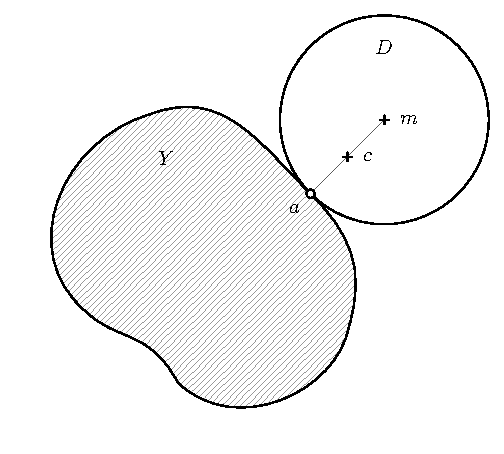
\includegraphics[width=.42\textwidth]{figures/fig06-tikz.pdf}\\图6\end{minipage}\end{center}
\sourcepage{185}
\subsection*{习题（第22节）}
\entry{22.1}{}
设$u\ge0$在$D(R)$调和。证明Harnack不等式$\frac{R-|z|}{R+|z|}u(0)\le u(z)\le\frac{R+|z|}{R-|z|}u(0)$。
\entry{22.2}{}
用Harnack不等式证明：整个复平面上有上界的实调和函数为常数。
\entry{22.3}{}
若连续实函数在$Y\subset\C$的每个闭圆盘上满足$u(a)\le\frac1{2\pi}\int_0^{2\pi}u(a+re^{i\theta})d\theta$，证明它次调和。
\entry{22.4}{}
若$a\in\partial Y$且存在从$a$出发的非退化线段$S$满足$S\cap Y=\varnothing$，证明$a$为正则边界点。

\section{可数拓扑}
\sourcepage{185}
本节证明Radó定理：每个黎曼曲面均有可数拓扑。紧情形显然。还将为后面构造非紧曲面的特殊穷竭。
\entry{23.1}{引理}
若连续开满射$f:X\to Y$的定义域有可数拓扑，则$Y$也有。
\begin{proof}
取$X$的可数基$\mathfrak U$，则$\{f(U):U\in\mathfrak U\}$为$Y$的基：若$y\in D$且$D$开，选$f(x)=y$，再取$x\in U\subset f^{-1}(D)$，则$y\in f(U)\subset D$。
\end{proof}
\sourcepage{186}
\entry{23.2}{Poincaré--Volterra引理}
若$X$为连通流形，$Y$为具有可数拓扑的Hausdorff空间，$f:X\to Y$连续且离散，则$X$有可数拓扑。
\begin{proof}
取$Y$的可数基$\mathfrak U$，令$\mathfrak B$为具有可数拓扑且为某$f^{-1}(U)$的连通分支的全部开集。

(a)$\mathfrak B$为基。给定$x\in D$、$D$开，由离散性，取相对紧开邻域$W\subset D$，使$\partial W$不遇$f^{-1}(f(x))$。则$f(\partial W)$紧闭且不含$f(x)$，可选$U\in\mathfrak U$含$f(x)$而避开此集。包含$x$的原像分支$V$不遇$\partial W$，故$V\subset W$，有可数拓扑，因而属于$\mathfrak B$。

(b)每个$V_0\in\mathfrak B$只遇到可数多个$V\in\mathfrak B$。对固定$U$，$f^{-1}(U)$的分支两两不交，$V_0$有可数拓扑，故只遇可数个分支；再用$\mathfrak U$可数。

(c)固定$V^*\in\mathfrak B$，令$\mathfrak B_n$为可从$V^*$经过$n$次非空交相邻的基开集链到达的所有基开集。由连通性，$\bigcup_n\mathfrak B_n=\mathfrak B$。$\mathfrak B_0=\{V^*\}$，由(b)归纳每个$\mathfrak B_n$可数，故整基可数。
\end{proof}
\entry{23.3}{Radó定理}
每个黎曼曲面有可数拓扑。
\begin{proof}
在坐标邻域$U$内取两不交闭圆盘$K_0,K_1$，令$Y:=X\setminus(K_0\cup K_1)$。由(22.18)，边界正则，因此存在调和函数$u$，在两边界分别为0、1。于是$\omega=d'u$为非零全纯形式。取万有覆盖$p:\widetilde Y\to Y$，$p^*\omega$有全纯原函数$f$。
\sourcepage{187}
$f$非常值，连续且离散，由(23.2)，$\widetilde Y$有可数拓扑；再由(23.1)，$Y$有可数拓扑。$X=Y\cup U$，故$X$亦然。
\end{proof}
为Runge逼近构造特殊穷竭，先定义一个包络算子。
\entry{23.4}{定义}
对$Y\subset X$，令$\Lambda(Y)$为$Y$与$X\setminus Y$的所有相对紧连通分支之并。若开集$Y=\Lambda(Y)$，称为\textbf{Runge开集}，即补集无紧连通分支。容易验证$\Lambda(\Lambda(Y))=\Lambda(Y)$；$Y_1\subset Y_2$则$\Lambda(Y_1)\subset\Lambda(Y_2)$。需要注明背景空间时写$\Lambda_X$。例如$Y=\{1<|z|<2\}$，则$\Lambda_\C(Y)=\{|z|<2\}$，而$\Lambda_{\C^*}(Y)=Y$。
\entry{23.5}{定理}
(i)$Y$闭则$\Lambda(Y)$闭；(ii)$Y$紧则$\Lambda(Y)$紧。
\begin{proof}
(i)设$C_j$为开集$X\setminus Y$的连通分支，均开。令$J_0$为相对紧分支的指标，则$X\setminus\Lambda(Y)=\bigcup_{j\notin J_0}C_j$开。

(ii)可设$Y\ne\varnothing$。取相对紧开邻域$U$包含$Y$。每个$C_j$都遇到$U$；否则其边界包含于$Y\subset U$而又须在$X\setminus U$，从而无边界，成为既开又闭的非空真子集，与连通性矛盾。
\sourcepage{188}
只有有限个$C_j$遇$\partial U$，因为紧集$\partial U$被不交开集$C_j$覆盖。相对紧分支中，未遇$\partial U$的全包含于$U$。因此$\Lambda(Y)$包含于$U$及有限个相对紧分支之并，相对紧；由(i)又闭，故紧。
\end{proof}
\entry{23.6}{推论}
非紧曲面有紧集列$K_j$满足(i)$\Lambda(K_j)=K_j$；(ii)$K_{j-1}\subset\operatorname{int}K_j$；(iii)$\bigcup_jK_j=X$。
\begin{proof}
先用可数拓扑取紧集穷竭$K_j'$。令$K_0=\Lambda(K_0')$。已构造到$m$时，取紧$M$使$K_m\cup K_m'\subset\operatorname{int}M$，令$K_{m+1}:=\Lambda(M)$。由(23.5)及包络性质得结论。
\end{proof}
\entry{23.7}{引理}
若紧集$K_1\subset\operatorname{int}K_2$且$\Lambda(K_2)=K_2$，则存在Runge开集$Y$使$K_1\subset Y\subset K_2$，且可选其边界正则。
\begin{proof}
对每个$x\in\partial K_2$，取不遇$K_1$的坐标邻域，并在其中取内部含$x$的闭圆盘。有限个这样的$D_1,\ldots,D_k$覆盖$\partial K_2$。令$Y:=K_2\setminus\bigcup_jD_j$，则开且有上述包含关系。$X\setminus K_2$各分支非相对紧；每个$D_j$连通且遇到至少一个这样的分支，故$X\setminus Y$也无相对紧分支。由(22.18)，边界点全部正则。
\end{proof}
\entry{23.8}{定理}
Runge开集的每个连通分支也为Runge开集。
\sourcepage{189}
\begin{proof}
设分支为$Y_i$，$A=X\setminus Y$，其分支$A_k$闭而非紧。可设$Y\ne X$。每个$\overline{Y_i}$都遇$A$；否则$Y_i$闭开，与连通性矛盾。$X\setminus Y_i$的每个分支$C$也遇$A$；否则它遇某$Y_j$（$j\ne i$），由$C$闭、$Y_j$连通得$\overline{Y_j}\subset C$，而$\overline{Y_j}$遇$A$，矛盾。故$C$包含某个完整的$A_k$，不能紧。因此$Y_i$为Runge开集。
\end{proof}
\entry{23.9}{定理}
非紧曲面有相对紧Runge区域穷竭$Y_0\Subset Y_1\Subset\cdots$，各边界正则。
\begin{proof}
只须使每个紧集$K$包含于这样的区域。先取连通紧$K_1\supset K$，再取紧$K_2$使$K_1\subset\operatorname{int}K_2$。由(23.7)在$K_1$与$\Lambda(K_2)$间取正则边界Runge开集，再取含$K_1$的连通分支；由(23.8)、(22.14)的注记仍Runge且边界正则。
\end{proof}
\subsection*{习题（第23节）}
\entry{23.1}{}
证明任意黎曼曲面万有覆盖的覆盖变换群可数。
\entry{23.2}{}
设$Y\subset\C$开，$K$为$\C\setminus Y$的紧连通分支。若多项式列在$Y$的各紧子集上一致收敛，证明它在$K$上一致收敛。
\entry{23.3}{}
若$Y\subset\C$上的每个全纯函数均可在紧子集上一致地由多项式逼近，证明$Y=\Lambda_\C(Y)$。

\section{Weyl引理}
\sourcepage{190}
本节引入广义函数——分布。分布总可求导，因而可以考虑分布意义下的微分方程解。Weyl引理断言，Laplace方程的分布解与通常解相同：每个调和分布均为光滑调和函数。
\entry{24.1}{}
对开集$X\subset\C$，令$\mathcal D(X):=\{f\in\mathcal E(X):\operatorname{Supp}f\text{在}X\text{中紧}\}$。定义$f_\nu\xrightarrow{\mathcal D}f$，如果(i)所有支集都包含于同一紧集$K\subset X$；(ii)对每个多重指标$\alpha=(\alpha_1,\alpha_2)\in\mathbb N^2$，$D^\alpha f_\nu$在$K$上一致趋于$D^\alpha f$，其中$D^\alpha:=\partial_x^{\alpha_1}\partial_y^{\alpha_2}$。这比逐点或一致收敛都强得多。
\entry{24.2}{定义}
\textbf{分布}是连续线性映射$T:\mathcal D(X)\to\C$。连续是指上述收敛蕴含$T[f_\nu]\to T[f]$。所有分布记为$\mathcal D'(X)$。
\entry{24.3}{例}
(a)连续函数$h$定义$T_h[f]:=\iint_Xh(z)f(z)dxdy$。
\sourcepage{191}
此映射线性连续，且若两连续函数给出相同分布，则两者相同。因此可把连续函数等同于其分布。
(b)点$a$定义Dirac分布$\delta_a[f]:=f(a)$，它不能由连续函数表示。
\entry{24.4}{分布的微分}
对光滑$h$及紧支集$f$，分部积分$|\alpha|=\alpha_1+\alpha_2$次得$\iint hD^\alpha f=(-1)^{|\alpha|}\iint fD^\alpha h$，无边界项。因此$T_{D^\alpha h}[f]=(-1)^{|\alpha|}T_h[D^\alpha f]$。一般定义
\[
(D^\alpha T)[f]:=(-1)^{|\alpha|}T[D^\alpha f].
\]
由求导保持$\mathcal D$收敛，此式仍定义分布；与通常导数相容。
\entry{24.5}{引理}
若$g:X\times I\to\C$光滑，$I\subset\R$开区间，$\operatorname{Supp}g\subset K\times I$且$K\Subset X$紧，则$t\mapsto T_z[g(z,t)]$光滑，且
\begin{equation}\frac d{dt}T_z[g(z,t)]=T_z[g_t(z,t)].\tag{*}\end{equation}
下标表示分布作用于$z$，将$t$视为参数。
\sourcepage{192}
\begin{proof}
只须证(*)，再反复应用。差商$f_h(z):=(g(z,t+h)-g(z,t))/h$在$\mathcal D(X)$中趋于$g_t(\cdot,t)$，故由$T$线性连续，差商经$T$作用后趋于右端。
\end{proof}
\entry{24.6}{引理}
若$g:X\times Y\to\C$光滑，支集于$K\times L$，其中$K\Subset X$、$L\Subset Y$紧，则
\[
T_z\left[\iint_Yg(z,\zeta)d\xi d\eta\right]=\iint_YT_z[g(z,\zeta)]d\xi d\eta,
\quad\zeta=\xi+i\eta.
\]
\begin{proof}
右端由(24.5)有定义。取含$L$的轴平行矩形$R$，将函数在外部延零。把两边各等分为$n$份，取子矩形代表点$\zeta_{n\nu}$，令$F$为$R$面积，则Riemann和$G_n(z):=(F/n^2)\sum_{\nu=1}^{n^2}g(z,\zeta_{n\nu})$在$\mathcal D(X)$中趋于左端括号中的积分。
\sourcepage{193}
由$T$连续，$T[G_n]$趋于左端，而同一Riemann和也趋于右端，故相等。
\end{proof}
\entry{24.7}{函数的光滑化}
选$\rho\in\mathcal D(\C)$，支集于单位圆盘，旋转不变，且$\iint\rho\,dxdy=1$。令$\rho_\varepsilon(z):=\varepsilon^{-2}\rho(z/\varepsilon)$，则支集于$|z|<\varepsilon$且积分仍为1。对开集$U$，令$U^{(\varepsilon)}:=\{z\in U:\overline{D(z,\varepsilon)}\subset U\}$，仍为开集。对连续$f$定义
\[
(\operatorname{sm}_\varepsilon f)(z):=\iint_U\rho_\varepsilon(z-\zeta)f(\zeta)d\xi d\eta.
\]
它在$U^{(\varepsilon)}$光滑，因为可积分号下求导，称为$f$的\textbf{光滑化}。定义当然依赖$\rho$的选择。
\entry{24.8}{引理}
对$f\in\mathcal E(U)$，(a)$D^\alpha\operatorname{sm}_\varepsilon f=\operatorname{sm}_\varepsilon(D^\alpha f)$；(b)若$f$在$D(z,\varepsilon)$调和，则$(\operatorname{sm}_\varepsilon f)(z)=f(z)$。
\sourcepage{194}
\begin{proof}
(a)平移变量写$\operatorname{sm}_\varepsilon f(z)=\iint_{|\zeta|<\varepsilon}\rho_\varepsilon(\zeta)f(z+\zeta)d\xi d\eta$，求导后再换回变量即得。
(b)调和函数满足圆周均值性质。由旋转不变性，极坐标积分给
\[
\operatorname{sm}_\varepsilon f(z)=\int_0^\varepsilon\rho_\varepsilon(r)r\left(\int_0^{2\pi}f(z+re^{i\theta})d\theta\right)dr
=2\pi f(z)\int_0^\varepsilon\rho_\varepsilon(r)rdr=f(z).
\]
\end{proof}
\entry{24.9}{定理（Weyl引理）}
若$T\in\mathcal D'(U)$且$\Delta T=0$，则$T$为光滑调和函数。即存在$h\in\mathcal E(U)$，$\Delta h=0$，使$T[f]=\iint_Uh f\,dxdy$对所有测试函数成立。
\sourcepage{195}
\begin{proof}
固定$\varepsilon>0$，对$z\in U^{(\varepsilon)}$令$h(z):=T_\zeta[\rho_\varepsilon(\zeta-z)]$。由(24.5)光滑，只须证明对支集于$U^{(\varepsilon)}$的$f$有$T[f]=\iint h f$。由(24.6)，
\[
T[\operatorname{sm}_\varepsilon f]=\iint_{U^{(\varepsilon)}}h(z)f(z)dxdy.
\]
由(13.3)存在整体光滑$\psi$满足$\Delta\psi=f$。在$V:=\C\setminus\operatorname{Supp}f$上$\psi$调和，故由(24.8.b)，$\psi=\operatorname{sm}_\varepsilon\psi$于$V^{(\varepsilon)}$。因此$\varphi:=\psi-\operatorname{sm}_\varepsilon\psi$有紧支集于$U$，且$\Delta\varphi=f-\operatorname{sm}_\varepsilon f$。由$\Delta T=0$，$T[\Delta\varphi]=0$，所以$T[f]=T[\operatorname{sm}_\varepsilon f]$，得证。
\end{proof}
\entry{24.10}{推论}
若$\partial T/\partial\bar z=0$，则$T$为全纯函数。
\begin{proof}$\Delta T=4\partial_z\partial_{\bar z}T=0$，由Weyl引理光滑，再由Cauchy--Riemann方程全纯。\end{proof}
\textbf{注记。}此证明几乎逐字适用于$\R^n$上的调和函数。Weyl引理是可微流形上椭圆微分算子一般正则性定理的特例，参见[35]、[43]。
\sourcepage{196}
\subsection*{习题（第24节）}
\entry{24.1}{}
定义分布列$T_\nu\to T$，若对每个$\varphi\in\mathcal D(X)$有$T_\nu[\varphi]\to T[\varphi]$。证明此时对每个$D^\alpha$都有$D^\alpha T_\nu\to D^\alpha T$。
\entry{24.2}{}
若连续函数列$f_\nu$满足对每个测试函数$\varphi$，$\iint f_\nu\varphi\to\iint f\varphi$，称其\textbf{弱收敛}于连续$f$。证明若各$f_\nu$调和（全纯），则极限$f$也调和（全纯）。

\section{Runge逼近定理}
\sourcepage{196--197}
经典Runge定理断言，复平面单连通区域上的全纯函数可在紧子集上一致地由整函数、从而由多项式逼近。Behnke--Stein[51]推广到任意非紧黎曼曲面：把单连通条件换为补集无紧连通分支。这里采用Malgrange[55]以Weyl引理为基础的泛函分析证明。
\entry{25.1}{}
在$\mathcal E(Y)$上引入Fréchet空间结构。选可数紧集族$K_j$覆盖$Y$，每个包含于坐标邻域$(U_j,z_j)$，$z_j=x_j+iy_j$。对$\nu\in\mathbb N^2$定义半范数$p_{j\nu}(f):=\sup_{a\in K_j}|D_j^\nu f(a)|$，$D_j^\nu=\partial_{x_j}^{\nu_1}\partial_{y_j}^{\nu_2}$。由$\{p_{j\nu}<\varepsilon\}$的有限交组成0的邻域基。收敛意味着函数及所有导数在每个紧集上一致收敛。此拓扑与所选紧集、坐标无关，使空间成为Fréchet空间。

在$\OO(Y)$上诱导的拓扑正是紧集上一致收敛拓扑，因为全纯函数的局部一致收敛蕴含所有导数的局部一致收敛。类似地，对$\omega=f_jd\bar z_j$定义$p_{j\nu}(\omega):=\sup_{K_j}|D_j^\nu f_j|$，得到$\mathcal E^{0,1}(Y)$的Fréchet结构。
\entry{25.2}{引理}
每个连续线性泛函$T:\mathcal E(Y)\to\C$都有紧支集：存在紧$K\subset Y$使$\operatorname{Supp}f\subset Y\setminus K$时$T[f]=0$。对$(0,1)$形式亦然。
\begin{proof}
由连续性，某0邻域上$|T[f]|<1$，其中含有限个半范数小球之交。令$K$为涉及的有限个$K_j$之并。若$f$支集避开$K$，则这些半范数对任意$\lambda f$均为零。故$|T[f]|<1/\lambda$对所有$\lambda>0$成立，只能为零。
\end{proof}
\entry{25.3}{引理}
设$Z\subset X$开，连续线性泛函$S:\mathcal E^{0,1}(X)\to\C$对每个紧支集于$Z$的$g$满足$S[d''g]=0$。
\sourcepage{198}
则存在$\sigma\in\Omega(Z)$使对每个紧支集于$Z$的$\omega$有$S[\omega]=\iint_Z\sigma\wedge\omega$。\translatornote{原文定理行写$\Omega(X)$，证明实际构造的是$\Omega(Z)$；此处按证明写出。}
\begin{proof}
取$Z$内坐标卡$U$，对$\varphi\in\mathcal D(U)$，把$\varphi d\bar z$在外部延零，记$\widetilde\varphi$。则$\varphi\mapsto S[\widetilde\varphi]$为分布，并在所有$\partial_{\bar z}g$上为零。由(24.10)，它由唯一全纯函数表示；吸收$dz\wedge d\bar z=-2i dxdy$的常因子后，写为$S[\widetilde\varphi]=\iint_Uh(z)\varphi(z)dz\wedge d\bar z$。令$\sigma_U=h dz$。

不同坐标卡上所得形式在交集对所有测试形式积分相同，故彼此相等，拼成$\sigma\in\Omega(Z)$。对任意紧支集形式，用单位分解为有限个坐标卡内支集的形式，再逐项相加即得。
\end{proof}
\sourcepage{199}
\entry{25.4}{定理}
设$Y\Subset X$为非紧黎曼曲面中的Runge开集。若$\overline Y\subset Y'\Subset X$开，则限制$\OO(Y')\to\OO(Y)$的像在紧集上一致收敛拓扑中稠密。
\begin{proof}
令$\beta:\mathcal E(Y')\to\mathcal E(Y)$为限制。由Hahn--Banach定理，只须证明：若连续线性泛函$T$在$\beta\OO(Y')$上为零，则在$\OO(Y)$上为零。

对$\omega\in\mathcal E^{0,1}(X)$，由(14.16)取$f\in\mathcal E(Y')$使$d''f=\omega|_{Y'}$，定义$S[\omega]:=T[f|_Y]$。两种$f$之差在$Y'$全纯，故定义无关选择。

为证$S$连续，令$V:=\{(\omega,f):d''f=\omega|_{Y'}\}\subset\mathcal E^{0,1}(X)\times\mathcal E(Y')$。它为闭子空间，因而Fréchet。投影$\operatorname{pr}_1:V\to\mathcal E^{0,1}(X)$满射，由Banach定理为开映射；而$S\operatorname{pr}_1=T\beta\operatorname{pr}_2$连续，故$S$连续。

由(25.2)，有紧集$K\subset Y$、$L\subset X$分别支承$T,S$。若$g$紧支集于$X\setminus K$，则$S[d''g]=T[g|_Y]=0$。由(25.3)，存在$\sigma\in\Omega(X\setminus K)$，使$S[\omega]=\iint\sigma\wedge\omega$对该开集内的紧支集形式成立。
\sourcepage{200}
由$S$支于$L$，$\sigma$在$X\setminus(K\cup L)$为零。$X\setminus\Lambda(K)$的每个分支均非相对紧，因而遇此集合。由恒等定理，$\sigma$在$X\setminus\Lambda(K)$为零，所以支集于此处的$\omega$有$S[\omega]=0$。

任取$f\in\OO(Y)$。由$Y$为Runge，$\Lambda(K)\subset Y$。选$g\in\mathcal E(X)$紧支集于$Y$且在$\Lambda(K)$附近等于$f$。则$T[f]=T[g|_Y]=S[d''g]$，而$d''g$支集避开$\Lambda(K)$，故此值为零。
\end{proof}
\entry{25.5}{Runge逼近定理}
非紧黎曼曲面$X$的开子集$Y$，若补集没有紧连通分支，则每个$Y$上的全纯函数均可在紧子集上一致地由$X$上的全纯函数逼近。
\begin{proof}
只须考虑$Y$相对紧的情形。给定$f\in\OO(Y)$、紧$K\subset Y$及$\varepsilon>0$，取Runge穷竭$Y_0:=Y\Subset Y_1\Subset\cdots$。由(25.4)取$f_1\in\OO(Y_1)$使$\|f_1-f\|_K<\varepsilon/2$。归纳取$f_n\in\OO(Y_n)$，使$n\ge2$时$\|f_n-f_{n-1}\|_{Y_{n-2}}<2^{-n}\varepsilon$。此列在每个$Y_n$上一致收敛于整体全纯$F$，由级数估计$\|F-f\|_K<\varepsilon$。
\end{proof}
\entry{25.6}{定理}
非紧黎曼曲面上每个$\omega\in\mathcal E^{0,1}(X)$都有$f\in\mathcal E(X)$满足$d''f=\omega$。
\begin{proof}
由(14.16)在每个相对紧开集上可解，仿照(13.2)作穷竭。
\sourcepage{201}
取Runge穷竭$Y_0\Subset Y_1\Subset\cdots$。归纳构造$f_n\in\mathcal E(Y_n)$，使$d''f_n=\omega$且$\|f_{n+1}-f_n\|_{Y_{n-1}}\le2^{-n}$。先任取$f_0$。若已到$n$，取$g_{n+1}$在$Y_{n+1}$上解方程。差$g_{n+1}-f_n$在$Y_n$全纯，由Runge定理取$h\in\OO(Y_{n+1})$使$\|(g_{n+1}-f_n)-h\|_{Y_{n-1}}\le2^{-n}$。令$f_{n+1}=g_{n+1}-h$。如(13.2)，局部解加上局部一致收敛的全纯修正级数，得到整体光滑极限$f$，且$d''f=\omega$。
\end{proof}
\subsection*{习题（第25节）}
\entry{25.1}{}
设连续线性泛函$S:\mathcal E^{(2)}(X)\to\C$对所有$g\in\mathcal E(X)$满足$S[d'd''g]=0$。证明存在调和$h$使对所有紧支集2形式有$S[\omega]=\iint_Xh\omega$。
\entry{25.2}{}
设$Y\subset\C$开。证明任给$g\in\mathcal E(Y)$，存在$f\in\mathcal E(Y)$使$\Delta f=g$。

\section{Mittag--Leffler定理与Weierstrass定理}
\sourcepage{201}
现在讨论非紧黎曼曲面上具有指定主部、或指定阶数零点与极点的亚纯函数的构造，这是平面Mittag--Leffler定理及Weierstrass定理的对应物。紧情形在第18、20节已讨论，可解需要附加条件；非紧情形则无此限制。
\sourcepage{202}
\entry{26.1}{定理}
非紧黎曼曲面满足$H^1(X,\OO)=0$。
\begin{proof}
由Dolbeault定理，$H^1(X,\OO)\cong\mathcal E^{0,1}(X)/d''\mathcal E(X)$，再由(25.6)商空间为零。
\end{proof}
\textbf{注记。}这是任意维Stein流形上Cartan--Serre定理B的特例，参见[32]、[34]。
\entry{26.2}{}
回顾(18.1)：开覆盖上的亚纯函数族$\mu=(f_i)$，若差$f_j-f_i$全纯，即为Mittag--Leffler分布。解为整体亚纯函数$f$，使$f-f_i$在各$U_i$全纯。差组成上闭链$(f_j-f_i)$，由(18.1)，可解当且仅当它为上边缘。因此由(26.1)得到：
\entry{26.3}{定理}
非紧黎曼曲面上的每个Mittag--Leffler分布均有解。

接着讨论Weierstrass乘积定理的对应物：给定除子$D$，求非零亚纯$f$使$(f)=D$。弱解的定义见(20.1)。
\entry{26.4}{引理}
非紧曲面上的每个除子均有弱解。
\begin{proof}
(a)由(23.6)，选紧集穷竭$K_j$满足$K_j=\Lambda(K_j)$及$K_j\subset\operatorname{int}K_{j+1}$。

(b)断言：若$a_0\notin K_j$，点除子$A_0$有在$K_j$恒为1的弱解。
\sourcepage{203}
因$a_0$所在的$X\setminus K_j$分支非相对紧，可选$a_1$在该分支且不属于$K_{j+1}$，再取避开$K_j$的从$a_1$到$a_0$的曲线$c_0$。由(20.5)，$\partial c_0$有在$K_j$为1的弱解$\varphi_0$。反复进行，得到$a_\nu\notin K_{j+\nu}$、避开$K_{j+\nu}$且从$a_{\nu+1}$到$a_\nu$的$c_\nu$，及$\partial c_\nu=A_\nu-A_{\nu+1}$的弱解$\varphi_\nu$，在$K_{j+\nu}$为1。有限积至$n$为$A_0-A_{n+1}$的弱解。无限积$\varphi:=\prod_{\nu=0}^\infty\varphi_\nu$在每个紧集上只有有限个非平凡因子，故收敛，正是$A_0$的所求弱解。

(c)对任意$D$，令$K_0=\varnothing$，定义$D_\nu$在$K_{\nu+1}\setminus K_\nu$上等于$D$，外部为零。各$D_\nu$仅有有限支集，且$D=\sum_\nu D_\nu$。由(b)及有限乘积、整数幂，取其弱解$\psi_\nu$在$K_\nu$为1。于是局部有限的乘积$\prod_\nu\psi_\nu$为$D$的弱解。
\end{proof}
\entry{26.5}{定理}
非紧黎曼曲面上的每个除子都是某个非零亚纯函数的除子。
\begin{proof}
局部可解，故选由单连通开集$U_i$组成的覆盖及$f_i\in\MM^*(U_i)$，使$(f_i)=D|_{U_i}$。则$f_i/f_j\in\OO^*(U_i\cap U_j)$。取(26.4)的弱解$\psi$，在$U_i$上写$\psi=\psi_i f_i$，其中$\psi_i$处处非零且可微。由单连通性存在光滑对数$\varphi_i$使$\psi_i=e^{\varphi_i}$。
\sourcepage{204}
于是$e^{\varphi_j-\varphi_i}=f_i/f_j$，故$\varphi_{ij}:=\varphi_j-\varphi_i$全纯，并满足上闭链关系。由$H^1(X,\OO)=0$，存在全纯$g_i$使$\varphi_j-\varphi_i=g_j-g_i$。因此$e^{g_i}f_i=e^{g_j}f_j$在交集成立，拼成整体亚纯$f$。其各局部除子等于$(f_i)$，故$(f)=D$。
\end{proof}
\entry{26.6}{推论}
每个非紧黎曼曲面上存在处处非零的全纯1形式。
\begin{proof}
取非常值亚纯函数$g$，由(26.5)取$f$使$(f)=-(dg)$，则$\omega:=f\,dg$全纯且无零点。
\end{proof}
\entry{26.7}{定理}
设$(a_\nu)$为无聚点的互异点列。任给$c_\nu\in\C$，存在$f\in\OO(X)$使$f(a_\nu)=c_\nu$。
\begin{proof}
由(26.5)取全纯$h$恰在各$a_\nu$有一阶零点。令$U_i:=X\setminus\bigcup_{\nu\ne i}\{a_\nu\}$，构成开覆盖。在$U_i$上令$g_i:=c_i/h$，则$i\ne j$时交集避开全部零点，故$(g_i)$为Mittag--Leffler分布。由(26.3)取解$g$，令$f:=gh$。在$U_i$上$f=c_i+(g-g_i)h$。
\sourcepage{205}
右端全纯，且在$a_i$值为$c_i$，得证。
\end{proof}
\entry{26.8}{推论}
每个非紧黎曼曲面均为\textbf{Stein流形}，即(i)任意不同两点可由整体全纯函数分离；(ii)对任一无聚点点列$(x_\nu)$，存在整体全纯$f$使$\limsup_\nu|f(x_\nu)|=\infty$。

\textbf{注记。}非紧黎曼曲面上的Mittag--Leffler、Weierstrass定理由H.~Florack[54]首次用Behnke--Stein[51]的方法证明。多复变中的对应问题，即第一、第二Cousin问题，在Stein流形理论的发展中起重要作用，参见[53]、[59]、[61]；用上同调求解这些问题也源于该理论。
\subsection*{习题（第26节）}
\entry{26.1}{}
证明非紧曲面上$H^1(X,\Omega)=0$。［提示：用(26.6)说明$\Omega\cong\OO$。］
\entry{26.2}{}
(a)任给$\omega\in\mathcal E^{(2)}(X)$，证明存在$f\in\mathcal E(X)$使$d'd''f=\omega$。
(b)若$\mathcal H$为调和函数层，证明$H^1(X,\mathcal H)=0$。
\entry{26.3}{}
证明非紧黎曼曲面上的每个亚纯函数都是两个全纯函数之商。
\entry{26.4}{}
设全纯$f,g$无共同零点。
(a)证明层序列$0\to\OO\xrightarrow\alpha\OO\oplus\OO\xrightarrow\beta\OO\to0$正合，其中$\alpha(\psi)=(\psi g,-\psi f)$、$\beta(\varphi_1,\varphi_2)=\varphi_1f+\varphi_2g$。
(b)证明存在整体全纯$\Phi,\Psi$使$\Phi f+\Psi g=1$。
\sourcepage{206}
\entry{26.5}{}
设$\mathfrak A=\sum_{j=1}^k\OO(X)f_j$为有限生成理想。证明它为主理想。［提示：令$D(x):=\min_j\operatorname{ord}_xf_j$，取$(f)=D$的全纯函数，验证$\mathfrak A=\OO(X)f$。］
\entry{26.6}{}
对非紧黎曼曲面上的任意除子$D$，证明(a)$H^1(X,\OO_D)=0$；(b)$H^1(X,\MM)=0$。

\section{Riemann映射定理}
\sourcepage{206}
Riemann映射定理断言：每个既不同构于$\PP^1$、也不同构于$\C$的单连通黎曼曲面，都双全纯于单位圆盘。因此任意黎曼曲面的万有覆盖总是这三种标准形之一。Riemann于1851年博士论文中提出此定理，但未给出最一般形式及完全严格的证明；完整证明由Poincaré与Koebe于1907年给出。
\entry{27.1}{}
定义“全纯”de Rham群$\operatorname{Rh}_{\mathrm{hol}}^1(X):=\Omega(X)/d\OO(X)$。单连通时每个全纯1形式都有原函数，故此群为零。我们将在这看似更弱的条件下证明映射定理，而定理又表明此条件蕴含单连通。
\entry{27.2}{引理}
若$\operatorname{Rh}_{\mathrm{hol}}^1(X)=0$，则(i)每个全纯$f:X\to\C^*$都有全纯对数与平方根；(ii)每个实调和函数为全纯函数的实部。
\begin{proof}
(i)$f^{-1}df$全纯，故等于$dg$。调整常数使某点$a$处$e^{g(a)}=f(a)$。
\sourcepage{207}
则$d(fe^{-g})=e^{-g}df-fe^{-g}f^{-1}df=0$，所以$fe^{-g}=1$。平方根取$e^{g/2}$。
(ii)由(19.4)，$du=\operatorname{Re}\omega$，而$\omega=dg$，所以$u=\operatorname{Re}g+\text{常数}$。
\end{proof}
\entry{27.3}{定理}
设$X$非紧，$Y\Subset X$为区域，$\operatorname{Rh}_{\mathrm{hol}}^1(Y)=0$，且边界正则。则$Y$双全纯于单位圆盘。
\begin{proof}
固定$a\in Y$。由Weierstrass定理，取$g\in\OO(X)$恰在$a$有一阶零点。解Dirichlet问题，取$\overline Y$上连续、内部调和的$u$，边界值为$\log|g|$。由(27.2)，$u=\operatorname{Re}h$，$h$全纯。令$f=e^{-h}g$。

在$Y\setminus\{a\}$有$|f|=\exp(\log|g|-u)$，故$|f|$延拓为$\overline Y$上连续函数$\varphi$，边界恒1。最大值原理给$|f|<1$于$Y$。对$r<1$，$f^{-1}(\{|z|\le r\})=\{y\in\overline Y:\varphi(y)\le r\}$是紧集且避开边界，故$f:Y\to D$固有。由(4.24)取值总重数恒定，而0恰取一次，所以$f$双射，从而双全纯。
\end{proof}
\entry{27.4}{}
通过穷竭可从上一定理推出一般定理，先准备若干工具。
\sourcepage{208}
记$D(r):=\{|z|<r\}$，允许$r=\infty$。Cauchy积分公式给出：若$f:D(r)\to D(r')$全纯，则$|f'(0)|\le r'/r$。
\entry{27.5}{引理}
若区域$G\subset\C$的补集有内点，$w_0\in G$，则全纯映射$f:D\to G$且$f(0)=w_0$所成的族，在紧集上一致收敛拓扑下是$\OO(D)$中的紧集。
\begin{proof}
取补集内点$a$，映射$z\mapsto1/(z-a)$把$G$双全纯映到某有限半径圆盘的子区域，结论由Montel定理得到。
\end{proof}
\entry{27.6}{定理}
所有单叶（即单射）全纯函数$f:D\to\C$，满足$f(0)=0$、$f'(0)=1$者构成紧族。
\begin{proof}
(a)给定序列$f_n$，令$r_n$为$D(r_n)\subset f_n(D)$的最大半径。逆映射$\varphi_n:D(r_n)\to D$满足$\varphi'_n(0)=1$，由(27.4)有$r_n\le1$。选$a_n\in\partial D(r_n)\setminus f_n(D)$，令$g_n=f_n/a_n$，则$D\subset g_n(D)$且$1\notin g_n(D)$。

(b)$g_n(D)$单连通，所以有全纯$\psi:g_n(D)\to\C^*$使$\psi(0)=i$、$\psi(z)^2=z-1$。令$h_n=\psi\circ g_n$。若$w,-w$均在$h_n(D)$，由平方相同与$g_n$单射，原像点相同，故$w=-w=0$，又推出$g_n=1$，矛盾。

(c)令$U=\psi(D)$；归一化使此$U$与$n$无关。由$D\subset g_n(D)$，$U\subset h_n(D)$，所以$h_n(D)$避开$-U$。由(27.5)，$h_n$有收敛子列。又$f_n=a_n(1+h_n^2)$且$|a_n|\le1$，故$f_n$也有收敛子列。
\sourcepage{209}
极限$f$满足$f(0)=0$、$f'(0)=1$，故非常值。

(d)须证$f$单叶。否则存在$a$使$f-a$至少有两个零点。选$r<1$使其在边界无零点，圆内按重数有$k\ge2$个零点，则$k=(2\pi i)^{-1}\int_{|z|=r}f'(z)/(f(z)-a)dz$。足够接近$f$的函数也取$a$共$k$次，与子列单叶矛盾。
\end{proof}
\entry{27.7}{引理}
若$Y$是$D(R)$的真子区域，$0\in Y$且$\operatorname{Rh}_{\mathrm{hol}}^1(Y)=0$，则存在$r<R$及全纯$f:Y\to D(r)$使$f(0)=0$、$f'(0)=1$。
\begin{proof}
先设$R<\infty$，缩放可设$R=1$。取$a\in D\setminus Y$，令$\varphi(z)=(z-a)/(1-\bar az)$。由(27.2)，存在$g$使$g^2=\varphi|_Y$，且$g(Y)\subset D$。令$b=g(0)$、$\psi(z)=(z-b)/(1-\bar bz)$、$h=\psi\circ g$。则$h(0)=0$，
\[
\gamma:=h'(0)=\frac1{1-|b|^2}\frac{1-|a|^2}{2b}=\frac{1+|b|^2}{2b},
\]
其中$b^2=-a$，故$|\gamma|>1$。取$r=1/|\gamma|$、$f=h/\gamma$。$R=\infty$情形类似处理。
\end{proof}
\entry{27.8}{引理}
若$X$非紧且$\operatorname{Rh}_{\mathrm{hol}}^1(X)=0$，则每个Runge区域$Y$也满足此条件。
\begin{proof}
取$\omega\in\Omega(Y)$，由(26.6)选$X$上无零点形式$\omega_0$，写$\omega=f\omega_0$。由Runge定理，取$f_n\in\OO(X)$在$Y$局部一致趋于$f$。
\sourcepage{210}
每个$f_n\omega_0$在$X$有原函数，故对$Y$的任意闭曲线积分为零。取极限得$\omega$所有周期为零，由(10.15)有原函数。
\end{proof}
\entry{27.9}{Riemann映射定理}
若$\operatorname{Rh}_{\mathrm{hol}}^1(X)=0$，则$X$双全纯于$\PP^1$、$\C$或$D$之一。

\textbf{注记。}单连通蕴含此条件；三种标准形均单连通，故逆命题也成立。
\begin{proof}
(a)$X$紧时$d\OO(X)=0$，故$\Omega(X)=0$，亏格为0，由(16.13)得球面。

(b)$X$非紧时，取边界正则的Runge穷竭$Y_0\Subset Y_1\Subset\cdots$。由(27.8)、(27.3)，各$Y_n$双全纯于圆盘。固定$a\in Y_0$及局部坐标$z$，可取$r_n>0$及双全纯$f_n:Y_n\to D(r_n)$，使$f_n(a)=0$、$df_n/dz(a)=1$。

(c)$h=f_{n+1}\circ f_n^{-1}$在0导数为1，由(27.4)，$1\le r_{n+1}/r_n$。令$R=\lim_nr_n\in(0,\infty]$。

(d)在$Y_0$上归一化$g_n(\zeta):=r_0^{-1}f_n(f_0^{-1}(r_0\zeta))$，是$D$上的归一化单叶函数。
\sourcepage{211}
由(27.6)可取子列在$Y_0$局部一致收敛，再在$Y_1,Y_2,\ldots$逐次选子列，取对角列，便在每个$Y_m$局部一致收敛。极限拼成$f\in\OO(X)$，单射且$f(a)=0$、$df/dz(a)=1$。

(e)显然$f(X)\subset D(R)$。若非满射，由(27.7)存在$r<R$及$g:f(X)\to D(r)$使$g(0)=0$、$g'(0)=1$。取$r_n>r$，则$g\circ f\circ f_n^{-1}:D(r_n)\to D(r)$在0导数为1，违反(27.4)。故$f$满射，定理得证。
\end{proof}
\entry{27.10}{}
按万有覆盖同构于$\PP^1$、$\C$、$D$，分别称曲面为\textbf{椭圆型、抛物型、双曲型}。覆盖变换群$G$作为万有覆盖的自同构群，无不动点且离散作用：(i)非恒等元素不固定任何点，由提升唯一性；(ii)每条轨道$Gx$为离散集，因为它恰为$p^{-1}(p(x))$。曲面就是万有覆盖模此群的商。
\sourcepage{212}
特别地，每个双曲型黎曼曲面均为圆盘模某个离散、无不动点自同构群的商。
\entry{27.11}{引理}
(a)球面的每个自同构都有不动点。
(b)$\C$的离散、无不动点自同构群必为以下之一：平凡群；按$n\gamma$（$n\in\Z$，$\gamma\ne0$）的全部平移；按$n\gamma_1+m\gamma_2$的全部平移，其中$\gamma_1,\gamma_2$实线性无关。
\begin{proof}
(a)球面自同构为分式线性变换$(az+b)/(cz+d)$，总有不动点。
(b)平面自同构为$az+b$。若$a\ne1$就有不动点，故群只由平移组成。0的轨道$\Gamma$为离散加法子群，在其张成的最小实子空间中由(21.1)为格；维数为0、1、2分别给出三种情形。
\end{proof}
\entry{27.12}{定理}
球面为椭圆型；平面、穿孔平面及所有复环面为抛物型；其余黎曼曲面均为双曲型。特别地，紧曲面按亏格0、1、$>1$对应这三型。
\sourcepage{213}
\textbf{注记。}亏格1紧曲面也称椭圆曲线，容易与上述术语混淆，因此很少把球面称为椭圆型黎曼曲面。
\begin{proof}
前两类显然。若万有覆盖为球面，由(27.11.a)及无不动点作用，群平凡，曲面即球面。若覆盖为$\C$，由(27.11.b)，三种群分别给出$\C$、$\C^*$、复环面；中间情形覆盖同构于$z\mapsto\exp(2\pi iz/\gamma)$。
\end{proof}
\entry{27.13}{Picard小定理}
非常值整函数取遍所有复值，至多遗漏一个。
\begin{proof}
若遗漏不同$a,b$，则可看作$f:\C\to X:=\C\setminus\{a,b\}$。$X$双曲，$f$提升到其圆盘万有覆盖。由Liouville定理提升为常数，故$f$常数，矛盾。
\end{proof}
\subsection*{习题（第27节）}
\entry{27.1}{}
设$f_\nu:X\to\C\setminus\{0,1\}$全纯，且某$x_0$处$f_\nu(x_0)$趋于$c\notin\{0,1\}$。证明存在子列在每个紧子集上一致趋于全纯$f:X\to\C\setminus\{0,1\}$。［提示：考虑到圆盘覆盖的适当提升并用Montel定理。］
\sourcepage{214}
\entry{27.2}{}
证明Picard大定理：若$f$在$0<|z|<r$全纯且0为本性奇点，则它取遍所有复值，至多遗漏一个。［提示：考虑$f_\nu(z)=f(2^{-\nu}z)$并用27.1。］\translatornote{原文写$f_\nu:U\to\C$、$f_\nu(z)=f(2^\nu z)$。对于固定穿孔圆盘$U$，后式一般未在整个$U$上定义；此处将指数改为$-\nu$。}

\section{具有指定自守加项的函数}
\sourcepage{214}
第10节中，微分形式积分产生加法自守函数，其加项确定周期同态$\pi_1(X)\to\C$。Behnke--Stein[51]证明：非紧曲面上任意这样的同态都可由全纯1形式的周期实现。本节证明此结论，同时讨论非常值自守加项。
\entry{28.1}{群的上同调}
设$G$为乘法群，$A$为$G$模，即加法阿贝尔群配作用$G\times A\to A$，满足$\sigma(a+b)=\sigma a+\sigma b$、$\sigma(\tau a)=(\sigma\tau)a$、$\varepsilon a=a$，其中$\varepsilon$为单位元。映射$\sigma\mapsto a_\sigma$称为\textbf{交叉同态}，如果$a_{\sigma\tau}=a_\sigma+\sigma a_\tau$。作用平凡时就是通常群同态。
\sourcepage{215}
交叉同态在逐项加法下构成群$Z^1(G,A)$。固定$f\in A$，令$a_\sigma=f-\sigma f$，则
\[
a_{\sigma\tau}=f-\sigma\tau f=(f-\sigma f)+\sigma(f-\tau f)=a_\sigma+\sigma a_\tau.
\]
如此得到的交叉同态称为上边缘，组成子群$B^1(G,A)$。定义第一群上同调$H^1(G,A):=Z^1(G,A)/B^1(G,A)$。
\entry{28.2}{自守加项}
设$p:Y\to X$为无分歧全纯覆盖，$G=\operatorname{Deck}(Y/X)$。令$\sigma f=f\circ\sigma^{-1}$，使$\OO(Y)$成为$G$模。差$a_\sigma:=f-\sigma f$称为$f$的自守加项，并构成交叉同态。若覆盖Galois且加项全零，则$f$属于$p^*\OO(X)$，可视为$X$上的函数。对亚纯、可微函数也可作相同定义。
\entry{28.3}{Galois覆盖}
每个$x$有连通开邻域$U$使$p^{-1}(U)=\coprod_{\lambda\in A}V_\lambda$，各限制为到$U$的同胚。固定$\lambda_0$，每个$\lambda$对应唯一$\sigma\in G$使$\sigma(V_{\lambda_0})=V_\lambda$。
\sourcepage{216}
对$y\in V_\lambda$令$\varphi(y):=(p(y),\sigma)$，得到保纤维同胚$p^{-1}(U)\to U\times G$，$G$取离散拓扑。它与群作用相容：$\varphi(y)=(x,\sigma)$则$\varphi(\tau y)=(x,\tau\sigma)$。这种同胚称为\textbf{$G$坐标卡}。写$\varphi=(p,\eta)$，则$\eta(\tau y)=\tau\eta(y)$。
\entry{28.4}{定理}
若$X,Y$非紧且$p:Y\to X$为无分歧全纯Galois覆盖，则每个交叉同态$G\to\OO(Y)$，$\sigma\mapsto a_\sigma$，均为某全纯函数$f$的自守加项。

\textbf{注记。}即$H^1(G,\OO(Y))=0$。对任意Stein流形亦成立，见Stein[62]、Serre[59]。
\begin{proof}
(a)取开覆盖$(U_i)$及$G$坐标卡$\varphi_i=(p,\eta_i)$。在$Y_i=p^{-1}(U_i)$上定义$f_i(y):=a_{\eta_i(y)}(y)$，显然全纯。
(b)断言$f_i-\sigma f_i=a_\sigma$。事实上，$(\sigma f_i)(y)=a_{\sigma^{-1}\eta_i(y)}(\sigma^{-1}y)$。
\sourcepage{217}
在交叉同态公式中取$\tau=\sigma^{-1}\eta_i(y)$，得$a_\sigma(y)=a_{\eta_i(y)}(y)-a_{\sigma^{-1}\eta_i(y)}(\sigma^{-1}y)$，即断言。

(c)差$g_{ij}:=f_i-f_j$在覆盖变换下不变，故下降为$U_i\cap U_j$上的全纯函数，满足上闭链关系。由$H^1(X,\OO)=0$，可写$g_{ij}=g_i-g_j$。把$g_i$拉回$Y_i$，则$\widetilde f_i:=f_i-g_i$仍有指定加项，且在交集上相同，因而拼成整体所求$f$。
\end{proof}
\entry{28.5}{定理}
对任意黎曼曲面的无分歧全纯Galois覆盖，每个交叉同态$G\to\mathcal E(Y)$均为某可微函数的自守加项。
\begin{proof}
同上，将$\OO$换为$\mathcal E$；任意曲面上$H^1(X,\mathcal E)=0$，无需非紧假设。
\end{proof}
\entry{28.6}{Behnke--Stein定理}
若$X$非紧，任给同态$\pi_1(X)\to\C$，$\sigma\mapsto a_\sigma$，存在$\omega\in\Omega(X)$使$\int_\sigma\omega=a_\sigma$。
\sourcepage{218}
\begin{proof}
在万有覆盖上，由(28.4)取有指定常加项的全纯函数$F$。由(10.13)，$dF$下降为具有这些周期的全纯1形式。
\end{proof}
\entry{28.7}{定理}
若$X$紧，则每个同态$\pi_1(X)\to\C$均由唯一调和1形式的周期实现。
\begin{proof}
由(28.5)如上构造闭1形式$\widetilde\omega$。由(19.12)，$\widetilde\omega=\omega+df$，其中$\omega$调和，周期不变。唯一性由(19.8)。
\end{proof}
\subsection*{习题（第28节）}
\entry{28.1}{}
证明任意黎曼曲面上$H^1(X,\C)\cong\operatorname{Hom}(\pi_1(X),\C)$。
\entry{28.2}{}
若$X$非紧，令$\operatorname{Rh}_{\mathrm{hol}}^1(X)=\Omega(X)/d\OO(X)$，证明$H^1(X,\C)\cong\operatorname{Rh}_{\mathrm{hol}}^1(X)$。
\entry{28.3}{}
任给整函数$g$，证明存在整函数$f$满足$f(z+1)=f(z)+g(z)$。［提示：考虑Galois覆盖$\mathrm{ex}(z)=e^{2\pi iz}$，构造合适交叉同态$\Z\to\OO(\C)$。］

\section{线丛与向量丛}
\sourcepage{219}
流形分析中常把每个点$x$与一个随$x$连续、或全纯变化的向量空间$E_x$联系起来，由此得到向量丛概念。
\entry{29.1}{定义}
设$p:E\to X$连续，各纤维$E_x=p^{-1}(x)$为$n$维复向量空间。若每点$a$有开邻域$U$及同胚$h:E_U:=p^{-1}(U)\to U\times\C^n$，满足(i)保纤维，即$\operatorname{pr}_1h=p$；(ii)在每个纤维上为线性同构，则称$p$为秩$n$的\textbf{向量丛}。$h$称\textbf{局部平凡化}或\textbf{线性坐标卡}。覆盖$(U_i)$上的局部平凡化族$(h_i)$称为图册。
\entry{29.2}{定义}
若有整体线性平凡化$h:E\to X\times\C^n$，称丛\textbf{平凡}。向量丛总局部平凡，概念的作用在于整体问题。
\entry{29.3}{定义}
秩1向量丛称为\textbf{线丛}。
\entry{29.4}{定理}
给定图册$h_i$，存在唯一连续映射$g_{ij}:U_i\cap U_j\to\operatorname{GL}(n,\C)$，使
\sourcepage{220}
$h_i h_j^{-1}(x,t)=(x,g_{ij}(x)t)$，且在三重交上$g_{ij}g_{jk}=g_{ik}$。这些$g_{ij}$称\textbf{转移函数}，其族为图册的上闭链。
\begin{proof}
$h_ih_j^{-1}$保纤维且逐纤维线性可逆，故唯一确定矩阵$g_{ij}(x)$；同胚连续性给矩阵连续。复合的恒等式直接给上闭链关系。
\end{proof}
\entry{29.5}{定义}
黎曼曲面上的向量丛图册，若所有转移函数全纯，称为\textbf{全纯图册}。两个图册若并集仍为全纯图册，称全纯相容。它是等价关系，其等价类称\textbf{全纯线性结构}。带此结构的向量丛称\textbf{全纯向量丛}。若结构中有只含一张整体坐标卡的图册，称\textbf{全纯平凡}。
\entry{29.6}{上闭链}
$U\mapsto\operatorname{GL}(n,\OO(U))$配限制构成群层，$n\ge2$时非阿贝尔。对覆盖$\mathfrak U$，
\sourcepage{221}
$Z^1(\mathfrak U,\operatorname{GL}(n,\OO))$表示满足$g_{ij}g_{jk}=g_{ik}$的矩阵族。$n\ge2$时，逐项相乘一般不使此集合成为群。全纯丛的转移函数构成这样的上闭链；反之也可由上闭链构造丛。
\entry{29.7}{定理}
每个$(g_{ij})\in Z^1(\mathfrak U,\operatorname{GL}(n,\OO))$均为某秩$n$全纯向量丛的一组全纯坐标卡的转移函数。
\begin{proof}
令$E':=\coprod_iU_i\times\C^n\times\{i\}$，用$X\times\C^n\times I$的诱导拓扑，$I$离散。定义$(x,t,i)\sim(x',t',j)$当且仅当$x=x'$且$t=g_{ij}(x)t'$。上闭链关系保证等价性。令$E=E'/\sim$，取商拓扑与商映射$\kappa$。投影诱导连续$p:E\to X$，各纤维自然为$n$维空间。$\kappa|_{U_i\times\C^n\times\{i\}}$为到$E_{U_i}$的同胚，取逆并省略$i$坐标得到$h_i$。按构造转移函数恰为$g_{ij}$。
\end{proof}
\entry{29.8}{定义}
$U\subset X$上的\textbf{截面}是连续$f:U\to E$，满足$p\circ f=\mathrm{id}_U$。
\sourcepage{222}
即$f(x)\in E_x$。在坐标卡$h_i$中有唯一连续表示$f_i:U_i\cap U\to\C^n$，满足$h_i(f(x))=(x,f_i(x))$。
\entry{29.9}{定义}
若各局部表示$f_i$全纯，称截面全纯；与所选全纯图册无关。全纯截面空间记$\OO_E(U)$，配限制构成层$\OO_E$。各表示满足
\begin{equation}f_i=g_{ij}f_j\quad\text{于 }U_i\cap U_j\cap U.\tag{*}\end{equation}
反过来，每个满足(*)的全纯$n$元函数族都定义截面。因此局部$\OO_E|_{U_i}\cong\OO^n|_{U_i}$；若丛整体全纯平凡，则$\OO_E\cong\OO^n$。
\entry{29.10}{全纯余切丛}
取坐标覆盖$(U_i,z_i)$，转移函数$g_{ij}:=dz_j/dz_i$全纯非零，满足上闭链关系，确定线丛$T^*(X)$，称\textbf{全纯余切丛}或\textbf{典范线丛}。其全纯截面层同构于$\Omega$：局部$\omega=f_i dz_i$的系数满足$f_i=(dz_j/dz_i)f_j$，恰为截面关系；反过来由系数拼成1形式。
\sourcepage{223}
\entry{29.11}{除子的线丛}
对除子$D$，选覆盖及亚纯$\psi_i$使$(\psi_i)=D|_{U_i}$。令$g_{ij}:=\psi_i/\psi_j\in\OO^*(U_i\cap U_j)$，定义线丛$E_D$。若$f\in\OO_D(U)$，则$f_i:=\psi_if$全纯且$f_i=g_{ij}f_j$，给出$E_D$截面；反之，满足此关系的$f_i$使$f_i/\psi_i$拼成$\OO_D(U)$中的亚纯函数。故$\OO_{E_D}\cong\OO_D$。

下面用不同于第14节的方法研究向量丛全纯截面层的上同调。
\entry{29.12}{引理}
设$Y\Subset X$开，$E$为全纯向量丛。对每个开集$Y_0\subset Y$，限制$H^1(Y,\OO_E)\to H^1(Y_0,\OO_E)$满射。
\begin{proof}
用有限个丛平凡化且双全纯于平面开集的$U_i$覆盖$Y$。对$V\subset U_i$，由(26.1)，$H^1(V,\OO_E)\cong H^1(V,\OO)^n=0$。令$Y_k:=Y_0\cup\bigcup_{i\le k}U_i$，只须逐步证明$H^1(Y_k)\to H^1(Y_{k-1})$满射。
\sourcepage{224}
令$V_i=U_i\cap Y_{k-1}$，$V_i'=V_i$（$i\ne k$），$V_k'=U_k$。两族分别为$Y_{k-1},Y_k$的Leray覆盖，且不同指标的交集不变。因此两个1上闭链集合相同，诱导的上同调映射满射。
\end{proof}
\entry{29.13}{定理}
若$Y\Subset X$开，则$H^1(Y,\OO_E)$有限维。
\begin{proof}
选$Y\Subset Y'\Subset X$及有限开集$V_i\Subset U_i$，分别覆盖$Y,Y'$；各$U_i$为平面开集且丛在其上全纯平凡。两覆盖$\mathfrak U,\mathfrak V$为Leray覆盖，由(29.12)限制在$H^1$上满射，故
\[
\varphi:C^0(\mathfrak V,\OO_E)\times Z^1(\mathfrak U,\OO_E)\to Z^1(\mathfrak V,\OO_E),\quad
(\eta,\xi)\mapsto\delta\eta+\beta\xi
\]
满射，其中$\beta$为限制。各局部截面空间用紧集上一致收敛拓扑成为Fréchet空间，上链取乘积拓扑，上闭链为闭子空间，故上述空间均为Fréchet。$\delta,\beta$连续；由Montel定理及相对紧性，$\beta$还是紧算子。

令$\psi(\eta,\xi):=\beta\xi$，则$\psi$紧。\translatornote{原文此处写作$\beta(\eta)$，但$\beta$的定义域是1上闭链空间，故应为$\beta(\xi)$。}由L.~Schwartz定理（附录B.11），满射减紧算子$\varphi-\psi$的像余维有限。
\sourcepage{225}
该像恰为$B^1(\mathfrak V,\OO_E)$，所以商$H^1(Y,\OO_E)$有限维。
\end{proof}
\entry{29.14}{推论}
紧黎曼曲面上的全纯向量丛满足$\dim H^1(X,\OO_E)<\infty$。
\entry{29.15}{亚纯截面}
局部平凡化下，穿孔邻域上的全纯截面由全纯$n$元函数表示。若各分量在$a$至多有$m$阶极点或可去奇点，且至少一项恰有$m$阶极点，称截面在$a$有$m$阶极点；定义与线性坐标无关。

开集$Y$上的\textbf{亚纯截面}，是$Y'\subset Y$上的全纯截面，其中$Y\setminus Y'$离散，且在所有缺失点均有极点。类似(14.12)可证明：
\entry{29.16}{定理}
对$Y\Subset X$及$a\in Y$，存在$Y$上的亚纯截面，在$a$有极点且在其他点全纯。
\entry{29.17}{推论}
紧曲面上的每个全纯向量丛都有非恒零的整体亚纯截面。
\entry{29.18}{线丛与除子}
若线丛$E$有非零整体亚纯截面$\psi$，其局部表示在各点的阶数定义除子$D$，与坐标无关。则$\OO_E\cong\OO_D$：若$(f)\ge-D$，$f\psi$全纯；反之，全纯截面$\varphi$的商$f=\varphi/\psi$为亚纯函数，满足该阶数条件。这可视为(29.11)的逆构造。
\sourcepage{226}
下面把紧曲面的Picard群解释为上同调群。
\entry{29.19}{定理}
自然有群同构$H^1(X,\OO^*)\cong\operatorname{Pic}(X)$。
\begin{proof}
(a)若$\xi$由$(g_{ij})$表示，取对应线丛$E$，由(29.17)有非零亚纯截面$f$，局部表示$f_i$满足$f_i=g_{ij}f_j$。它的除子$D(x)=\operatorname{ord}_xf_i$良定义，定义$\alpha(\xi):=D\bmod\operatorname{Div}_p$。

若同一上闭链也写为$g_{ij}=\widetilde f_i/\widetilde f_j$，则$f_i/\widetilde f_i$拼成整体非零亚纯$\varphi$，故两除子相差主除子$(\varphi)$。与代表上闭链选择无关的验证留给读者。容易看出$\alpha$为群同态。

(b)由(29.11)满射。若$D$为主除子，取亚纯$\varphi$使$(\varphi)=D$，
\sourcepage{227}
则$g_i:=f_i/\varphi\in\OO^*(U_i)$，$g_{ij}=g_i/g_j$，故上闭链为上边缘，得到单射。
\end{proof}
\subsection*{习题（第29节）}
\entry{29.1}{}
秩$n$全纯向量丛的\textbf{秩$k$全纯子丛}$F\subset E$，是局部可用全纯平凡化写成$h(F_U)=U\times(\C^k\times0)$的子集。
(a)若$f$为处处非零的全纯截面，令$F_x=\C f(x)$，证明$\bigcup_xF_x$为秩1子丛。
(b)若$f$为亚纯截面，证明存在唯一秩1子丛使$f$为其亚纯截面。\translatornote{本小问题意需要$f$非恒零；零截面一般不能确定唯一线子丛。}
\entry{29.2}{}
紧曲面上线丛的次数定义为非零亚纯截面除子的次数。
(a)证明此定义与截面选择无关。
(b)在球面上取$U_1=\{|z|<1+\varepsilon\}$、$U_2=\{|z|>1-\varepsilon\}$（包含$\infty$），$0<\varepsilon<1$。若线丛由转移函数$g_{12}\in\OO^*(U_1\cap U_2)$给出，证明$\deg L=(2\pi i)^{-1}\int_{|z|=1}g'_{12}(z)/g_{12}(z)dz$。［提示：先考虑$g_{12}(z)=z^k$。］

\section{向量丛的平凡性}
\sourcepage{228}
本节证明非紧黎曼曲面上的每个全纯向量丛均平凡，下一节据此解决Riemann--Hilbert问题。
\entry{30.1}{定理}
设$E$秩为$n$，图册$(h_i)$的转移上闭链为$(g_{ij})$。以下等价：(i)$E$全纯平凡；(ii)存在$n$个整体全纯截面$F_1,\ldots,F_n$，每个纤维中取值线性无关；(iii)上闭链可分裂，即存在$g_i\in\operatorname{GL}(n,\OO(U_i))$使$g_{ij}=g_ig_j^{-1}$。
\begin{proof}
(i)推出(ii)：在整体平凡化下取常标准基向量的原像。
(ii)推出(iii)：令$g_i$的各列为$F_\nu$在$h_i$下的局部表示。逐纤维独立保证矩阵可逆，截面关系给$g_i=g_{ij}g_j$。
(iii)推出(i)：若$h_i(v)=(x,t)$，定义$h(v):=(x,g_i^{-1}t)$。在另一坐标中$t=g_{ij}t'=g_ig_j^{-1}t'$，故定义无关选择，且$h$与所有$h_i$全纯相容，是整体平凡化。
\end{proof}
\entry{30.2}{引理}
非紧曲面上的全纯向量丛若有非零整体亚纯截面，则有处处非零的整体全纯截面。
\sourcepage{229}
\begin{proof}
设$f$为亚纯截面，$A$为其零点、极点的离散集。在$a\in A$附近将$f$表示为$(f_1,\ldots,f_n)$，令$k(a):=\min_i\operatorname{ord}_af_i$。由Weierstrass定理，取亚纯$\varphi$在$a$处阶数$-k(a)$，在$X\setminus A$全纯非零。则$F=\varphi f$全纯且无零点。
\end{proof}
\entry{30.3}{定理}
非紧黎曼曲面上的每个全纯线丛均全纯平凡。
\begin{proof}
取非空Runge穷竭$Y_0\Subset Y_1\Subset\cdots$。由(29.16)、(30.2)，每个$Y_n$上有无零点全纯截面，故丛在其上平凡。由Runge定理，$Y_n$上的截面可在紧集上由$Y_{n+1}$上的截面逼近。选$f_0$在某$a\in Y_0$非零，逐次逼近使$f_n$在每个$Y_\nu$上收敛，且$f_n(a)$的极限非零。得到非恒零整体全纯截面，再用(30.2)、(30.1)得整体平凡。
\end{proof}
\entry{30.4}{定理}
非紧黎曼曲面上的每个全纯向量丛均全纯平凡。
\begin{proof}
对秩$n$归纳，$n=1$已证，设秩$n-1$时成立。

(a)先假设存在处处非零全纯截面$F_n$。局部补成标架，以列向量$F^i$表示其余$n-1$个截面。在交集上
\begin{equation}F^i=G_{ij}F^j+a_{ij}F_n,\tag{1}\end{equation}
其中$G_{ij}\in\operatorname{GL}(n-1,\OO(U_i\cap U_j))$，$a_{ij}$为$n-1$行列向量。由标架关系$G_{ij}G_{jk}=G_{ik}$。
\sourcepage{230}
由归纳假设，$G_{ij}=G_iG_j^{-1}$。令$\widetilde F^i=G_i^{-1}F^i$，则
\begin{equation}\widetilde F^i=\widetilde F^j+b_{ij}F_n.\tag{2}\end{equation}
系数满足$b_{ij}+b_{jk}=b_{ik}$。由$H^1(X,\OO)=0$，取$b_i$使$b_{ij}=b_i-b_j$。于是$\widetilde F^i-b_iF_n$在交集上相同，拼成$n-1$个整体截面，与$F_n$逐纤维独立，故丛平凡。

(b)还需构造无零点截面。由(29.16)、(30.2)，在任意相对紧区域上存在这样的截面，由(a)丛在那里平凡。与(30.3)一样，用Runge逼近及穷竭构造非恒零整体全纯截面，再由(30.2)消去其零点。
\end{proof}
\entry{30.5}{推论}
若$X$非紧，则$H^1(X,\operatorname{GL}(n,\OO))=0$，特别地$H^1(X,\OO^*)=0$。
\begin{proof}
这里第一上同调为零表示每个开覆盖上的每个矩阵上闭链均可分裂，由(30.1)恰等价于全纯向量丛平凡。
\end{proof}
\subsection*{习题（第30节）}
\entry{30.1}{}
证明任意黎曼曲面，无论紧与否，均有$H^1(X,\MM^*)=0$。［提示：用习题16.4的正合序列。］
\entry{30.2}{}
$U\mapsto\operatorname{SL}(n,\OO(U))$配限制为群层。
\sourcepage{231}
证明非紧曲面上$H^1(X,\operatorname{SL}(n,\OO))=0$，即每个该群层上闭链均可写为$g_{ij}=g_ig_j^{-1}$，且各$g_i$行列式为1。

\section{Riemann--Hilbert问题}
\sourcepage{231}
第11节中，线性微分方程基本解系的自守行为给出同态$T:\pi_1(X)\to\operatorname{GL}(n,\C)$。反过来，给定此同态，能否找到微分方程，使解沿闭曲线解析延拓时恰按指定自守因子变化？这就是\textbf{Riemann--Hilbert问题}。本节用H.~Röhrl[57]的方法给出非紧黎曼曲面上的解。
\entry{31.1}{自守因子}
设$p:Y\to X$为无分歧全纯覆盖，$G=\operatorname{Deck}(Y/X)$。若全纯$\Phi:Y\to\operatorname{GL}(n,\C)$满足$\sigma\Phi=\Phi T_\sigma$，其中$T_\sigma$为常可逆矩阵，则称具有常自守因子的乘法自守函数。由(11.6)，$\sigma\mapsto T_\sigma$为群同态。下一定理对应(28.4)。
\entry{31.2}{定理}
若$X,Y$非紧，$p:Y\to X$为无分歧全纯Galois覆盖，则对每个同态$T:G\to\operatorname{GL}(n,\C)$，存在全纯$\Phi$使$\sigma\Phi=\Phi T_\sigma$。
\sourcepage{232}
\begin{proof}
(a)取开覆盖及$G$坐标卡$\varphi_i=(p,\eta_i)$，在$Y_i=p^{-1}(U_i)$上定义$\Psi_i(y):=T_{\eta_i(y)}^{-1}$。它局部常值，因而全纯。

(b)由$\eta_i(\sigma^{-1}y)=\sigma^{-1}\eta_i(y)$，得
\[
(\sigma\Psi_i)(y)=T_{\sigma^{-1}\eta_i(y)}^{-1}=T_{\eta_i(y)}^{-1}T_\sigma=\Psi_i(y)T_\sigma.
\]
(c)$F_{ij}:=\Psi_i\Psi_j^{-1}$在覆盖变换下不变，下降到$U_i\cap U_j$，构成矩阵上闭链。由(30.5)，$F_{ij}=F_iF_j^{-1}$，其中$F_i$全纯可逆。拉回这些矩阵，令$\Phi_i:=F_i^{-1}\Psi_i$，则$\sigma\Phi_i=\Phi_iT_\sigma$，且
\[
\Phi_i^{-1}\Phi_j=\Psi_i^{-1}F_iF_j^{-1}\Psi_j=\Psi_i^{-1}F_{ij}\Psi_j=I.
\]
故拼成所求整体$\Phi$。
\end{proof}
\entry{31.3}{推论}
非紧曲面上任给同态$T:\pi_1(X)\to\operatorname{GL}(n,\C)$，存在$A\in M(n\times n,\Omega(X))$，使$dw=Aw$在万有覆盖上有自守因子为$T_\sigma$的基本解系。
\begin{proof}
对万有覆盖应用(31.2)，再用(11.6)。
\end{proof}
\entry{31.4}{}
设$X$为非紧黎曼曲面。若$S\subset X$闭离散，$X':=X\setminus S$，可对$X'$应用上述推论。但还希望所构造方程在每个$a\in S$至多有正则奇点，先准备引理。
\sourcepage{233}
\textbf{引理。}设$p:Y\to X'$为万有覆盖，$(U,z)$为$a\in S$的坐标邻域，$z(U)=D$、$z(a)=0$、$U\cap S=\{a\}$。则$p^{-1}(U\setminus\{a\})$的每个连通分支$Z$，都以$p|_Z$成为$U\setminus\{a\}$的万有覆盖。
\begin{proof}
由Weierstrass定理，取$X$上恰在$a$有一阶零点的全纯函数$f$。则$\omega=df/f$在$X'$全纯，沿绕$a$一周的正向小圆$\gamma$有积分$2\pi i$。若$p|_Z$不是万有覆盖，由(5.10)它同构于某$k$次幂覆盖。此时$\gamma$可连续提升$k$次形成闭曲线$c$，于是$\int_c p^*\omega=2k\pi i$。但$p^*\omega$在单连通$Y$上有原函数，闭曲线积分必须为零，矛盾。
\end{proof}
现在对$X'$上方程$dw=Aw$及基本解系$\Phi$，若在每个这样的分支$Z$上，$\Phi|_Z$都满足(11.12)的条件，则称方程在$a$有正则奇点。
\entry{31.5}{定理}
设$X$非紧，$S$闭离散，$X'=X\setminus S$。任给同态$T:\pi_1(X')\to\operatorname{GL}(n,\C)$，
\sourcepage{234}
存在$A\in M(n\times n,\Omega(X'))$，使$dw=Aw$在$S$的各点有正则奇点，且在万有覆盖$p:Y\to X'$上有基本解系$\Phi$，满足$\sigma\Phi=\Phi T_\sigma$。
\begin{proof}
设$S=\{a_i:i\in I\}$，取满足(31.4)条件的坐标邻域$(U_i,z_i)$。令$0\notin I$，$J=I\cup\{0\}$，$U_0=X'$，则为$X$的开覆盖，不同指标的交集在$X'$中。令$Y_0=Y$、$Y_i=p^{-1}(U_i\setminus\{a_i\})$。

由(31.2)取$\Psi_0\in\operatorname{GL}(n,\OO(Y))$有指定自守因子。由(11.10)，各$Y_i$上可取有正则奇点且与$\Psi_0$自守行为相同的$\Psi_i$。于是$F_{ij}:=\Psi_i\Psi_j^{-1}$在覆盖变换下不变，可视为$U_i\cap U_j$上的全纯可逆矩阵，令$F_{jj}=I$，得到矩阵上闭链。由$H^1(X,\operatorname{GL}(n,\OO))=0$，写$F_{ij}=F_iF_j^{-1}$。

令$\Phi_i:=F_i^{-1}\Psi_i$，如(31.2)拼成整体$\Phi$，满足指定自守行为。因$F_i^{-1}$在整个$U_i$全纯，乘上它不破坏$\Psi_i$的正则奇点性质。最后$A:=d\Phi\cdot\Phi^{-1}$在覆盖变换下不变，下降为$X'$上的全纯1形式矩阵，故$\Phi$为所求基本解系。\translatornote{原文证明末尾把定义域和基本群写为$X$；按定理及构造，此处应为$X'$。}
\end{proof}
\subsection*{习题（第31节）}
\entry{31.1}{}
设$p:Y\to X$为非紧曲面间的无分歧全纯Galois覆盖，$G=\operatorname{Deck}(Y/X)$。设$a:G\to\operatorname{GL}(n,\OO(Y))$为交叉同态，满足$a_{\sigma\tau}=a_\sigma(\sigma a_\tau)$。
\sourcepage{235}
证明存在全纯可逆矩阵$\Phi$使$a_\sigma=\Phi(\sigma\Phi)^{-1}$。
\entry{31.2}{}
任给全纯可逆矩阵$g:\C\to\operatorname{GL}(n,\C)$，证明存在全纯可逆矩阵$f$使$f(z+1)=f(z)g(z)$。［提示：对覆盖$z\mapsto e^{2\pi iz}$应用31.1。］

\backmatter
\chapter*{附录}
\markboth{附录}{附录}
\addcontentsline{toc}{chapter}{附录}
\section*{A. 单位分解}
\sourcepage{237}
单位分解是可微流形研究的重要工具，本书多次使用。本附录汇集有关主要事实，证明可参见[40]、[43]、[45]、[48]。
\entry{A.1}{}
函数$f$的支集$\operatorname{Supp}f$是$\{x:f(x)\ne0\}$的闭包。支集恰为半径$\varepsilon$闭球的标准$C^\infty$实函数为
\[
g(x):=\begin{cases}\exp\bigl(-1/(\varepsilon^2-\|x\|^2)\bigr),&\|x\|<\varepsilon,\\0,&\|x\|\ge\varepsilon,\end{cases}
\qquad\|x\|=\left(\sum_{j=1}^n|x_j|^2\right)^{1/2}.
\]
由它可构造所需的其他光滑函数。
\entry{A.2}{}
$n$维流形为每点有邻域同胚于$\R^n$开集的Hausdorff空间。同胚$\varphi:U\to V$称坐标卡。若转移映射$\varphi_2\varphi_1^{-1}$及其逆均无限次可微，称两卡可微相容。
\sourcepage{238}
如第1节定义黎曼曲面那样，以可微相容代替双全纯相容，即得到可微流形。黎曼曲面尤其是二维可微流形。在每张坐标卡下均$C^\infty$的函数称为可微函数。
\entry{A.3}{定义}
从属于开覆盖$\mathfrak U=(U_i)$的\textbf{可微单位分解}是可微函数族$g_i:X\to\R$，满足(i)$0\le g_i\le1$；(ii)$\operatorname{Supp}g_i\subset U_i$；(iii)支集族局部有限，即每点有邻域仅遇有限多个支集；(iv)$\sum_ig_i=1$。由(iii)，求和良定义。
\entry{A.4}{定理}
具有可数拓扑的可微流形上，每个开覆盖均有从属的可微单位分解。
\entry{A.5}{推论}
对可微流形中的紧集$K$及其开邻域$V$，存在可微实函数$f$，使$\operatorname{Supp}f\Subset V$、$f|_K=1$。
\begin{proof}
可假设$X$有可数拓扑，否则在$K$的相对紧开邻域中工作。取$K\subset U_1\Subset V$、$U_2=X\setminus K$，取从属单位分解$(g_1,g_2)$，令$f=g_1$。
\end{proof}
\section*{B. 拓扑向量空间}
这里陈述本书用到的泛函分析概念与事实，细节及证明见[44]、[47]。
\sourcepage{239}
\entry{B.1}{}
以下向量空间均为复向量空间。\textbf{拓扑向量空间}是带拓扑的向量空间$E$，使加法$E\times E\to E$与数乘$\C\times E\to E$连续。每个平移$x\mapsto a+x$为同胚，因此拓扑由0的邻域基完全确定；$a+U$给出$a$的邻域基。
\entry{B.2}{半范数}
映射$p:E\to\R$若满足三角不等式$p(x+y)\le p(x)+p(y)$及$p(\lambda x)=|\lambda|p(x)$，称为半范数。必有$p(x)\ge0$；若仅在$x=0$为零，则称范数。

半范数族$(p_i)$诱导拓扑，其0邻域基为$\{x:\max(p_{i_1}(x),\ldots,p_{i_m}(x))<\varepsilon\}$。此拓扑Hausdorff当且仅当所有$p_i(x)=0$蕴含$x=0$。可由半范数族如此诱导拓扑的空间称为\textbf{局部凸}空间。
\entry{B.3}{Fréchet空间}
若对每个0邻域$U$，存在$n_0$使$n,m\ge n_0$时$x_n-x_m\in U$，称$(x_n)$为Cauchy列。若(i)拓扑Hausdorff且由可数个半范数定义；(ii)每个Cauchy列收敛，则称为\textbf{Fréchet空间}。它可度量化：若$(p_n)$定义拓扑，则
\[
d(x,y):=\sum_{n=0}^\infty2^{-n}\frac{p_n(x-y)}{1+p_n(x-y)}
\]
\sourcepage{240}
为诱导同一拓扑的度量。闭向量子空间仍为Fréchet空间，可数个Fréchet空间的乘积亦然。
\entry{B.4}{}
典型例子是平面开集上$\OO(X)$，取紧集上一致收敛拓扑；由半范数$p_K(f):=\sup_K|f|$定义。只需可数紧集穷竭$(K_n)$对应的半范数即可定义此拓扑。
\entry{B.5}{Banach空间与Hilbert空间}
完备赋范空间称为\textbf{Banach空间}，即拓扑由单一范数定义的Fréchet空间。若范数来自内积，$\|x\|=\sqrt{\langle x,x\rangle}$，则称\textbf{Hilbert空间}。子空间$A$的正交补$A^\perp:=\{y:\langle y,x\rangle=0\text{ 对所有 }x\in A\}$闭；若$A$本身闭，则$E=A\oplus A^\perp$。
\entry{B.6}{Banach定理}
Fréchet空间之间的连续线性满射为开映射。
\entry{B.7}{推论}
Banach空间之间的连续线性满射$f:E\to F$存在常数$C>0$，使每个$y\in F$有原像$x$满足$\|x\|\le C\|y\|$。
\begin{proof}
令$U=\{\|x\|<1\}$。开映射定理给$\varepsilon>0$使$f(U)\supset\{\|y\|<\varepsilon\}$。取$C=2/\varepsilon$。$y=0$时取$x=0$；否则令$\lambda=\|y\|$，$y_1=y/(\lambda C)$落在此球中，故有$x_1\in U$使$f(x_1)=y_1$。
\sourcepage{241}
取$x=\lambda Cx_1$，即得$f(x)=y$及范数估计。
\end{proof}
\entry{B.8}{Hahn--Banach定理}
局部凸空间$E$的子空间$E_0$上的每个连续线性泛函$\varphi_0:E_0\to\C$都可延拓为$E$上的连续线性泛函。
\entry{B.9}{推论}
设$E$为局部凸拓扑向量空间。若$A\subset B\subset E$为向量子空间，而在$A$上为零的每个连续线性泛函都在$B$上为零，则$A$在$B$中稠密。
\begin{proof}
否则取$b_0\in B\setminus\overline A$，在$E_0=A\oplus\C b_0$上令$\varphi_0(a+\lambda b_0)=\lambda$。它连续，延拓后在$A$为零而在$b_0$不为零，矛盾。
\end{proof}
\entry{B.10}{紧映射}
线性映射$\psi:E\to F$若把某0邻域映为相对紧集，称为\textbf{紧映射}或\textbf{完全连续映射}。特别地，紧线性映射连续。

\textbf{例。}若$Y\Subset X\subset\C$开，则限制$\beta:\OO(X)\to\OO(Y)$紧。事实上，$U:=\{f:\sup_{\overline Y}|f|<1\}$为0邻域，由Montel定理，$M:=\{g\in\OO(Y):\sup_Y|g|\le1\}$紧，而$\beta(U)\subset M$。
\entry{B.11}{L. Schwartz定理}
设$E,F$为Fréchet空间，$\varphi,\psi:E\to F$连续线性，$\varphi$满射且$\psi$紧。则$\varphi-\psi$的像在$F$中余维有限。证明见[60]。

\chapter*{参考文献}
\markboth{参考文献}{参考文献}
\addcontentsline{toc}{chapter}{参考文献}
\sourcepage{243--245}
以下保留原书文献编号、作者姓名及出版资料；中文题名后列原题名，便于检索。
\section*{(a) 单复变函数论}
\begin{description}[style=nextline,leftmargin=2em]
\item[{[1]}] Ahlfors, L. V.：《复分析》（Complex Analysis）。New York: McGraw-Hill, 1966。
\item[{[2]}] Behnke, H.; Sommer, F.：《单复变解析函数论》（Theorie der analytischen Funktionen einer komplexen Veränderlichen），第3版。Berlin--Heidelberg--New York: Springer, 1965。
\item[{[3]}] Cartan, H.：《单复变与多复变解析函数初等理论》（Elementary Theory of Analytic Functions of One or Several Complex Variables）。Reading, MA: Addison-Wesley, 1963。
\item[{[4]}] Hurwitz, A.; Courant, R.：《函数论》（Funktionentheorie），附录由 H. Röhrl 撰写，第4版。Berlin--Heidelberg--New York: Springer, 1964。
\item[{[5]}] Lang, S.：《复分析》（Complex Analysis）。Reading, MA: Addison-Wesley, 1977。
\end{description}
Behnke--Sommer 和 Hurwitz--Courant 两书中有相当大的篇幅讨论黎曼曲面。
\section*{(b) 黎曼曲面}
\begin{description}[style=nextline,leftmargin=2em]
\item[{[10]}] Ahlfors, L. V.; Sario, L.：《黎曼曲面》（Riemann Surfaces）。Princeton, NJ: University Press, 1960。
\item[{[11]}] Chevalley, C.：《单变量代数函数论导引》（Introduction to the Theory of Algebraic Functions of One Variable）。American Mathematical Society, 1951。
\item[{[12]}] Farkas, H. M.; Kra, I.：《黎曼曲面》（Riemann Surfaces）。New York--Heidelberg--Berlin: Springer, 1980。
\item[{[13]}] Guenot, J.; Narasimhan, R.：《黎曼曲面论导引》（Introduction à la Théorie des Surfaces de Riemann）。Monographies de l'Enseignement Mathématique 23, Genève, 1976。
\item[{[14]}] Gunning, R. C.：《黎曼曲面讲义》（Lectures on Riemann Surfaces）。Princeton Mathematical Notes 2 (1966)。
\item[{[15]}] Gunning, R. C.：《黎曼曲面上的向量丛讲义》（Lectures on Vector Bundles over Riemann Surfaces）。Princeton Mathematical Notes 6 (1967)。
\item[{[16]}] Gunning, R. C.：《黎曼曲面讲义：雅可比簇》（Lectures on Riemann Surfaces: Jacobi Varieties）。Princeton Mathematical Notes 12 (1972)。
\item[{[17]}] Nevanlinna, R.：《单值化》（Uniformisierung）。Berlin--Heidelberg--New York: Springer, 1953。
\item[{[18]}] Pfluger, A.：《黎曼曲面论》（Theorie der Riemannschen Flächen）。Berlin--Heidelberg--New York: Springer, 1957。
\item[{[19]}] Serre, J.-P.：《代数群与类域》（Groupes Algébriques et Corps de Classes）。Paris: Hermann, 1959。
\item[{[20]}] Springer, G.：《黎曼曲面导论》（Introduction to Riemann Surfaces）。Reading, MA: Addison-Wesley, 1957。
\item[{[21]}] Weyl, H.：《黎曼曲面的概念》（The Concept of a Riemann Surface）。Reading, MA: Addison-Wesley, 1955。
\end{description}
Weyl 的书于1913年首次以德文出版，是第一部以现代方式处理黎曼曲面的著作，至今仍值得一读；其中还有许多十九世纪文献的引述。Chevalley 和 Serre 的书从代数的观点研究黎曼曲面。
\section*{(c) 多复变分析与复流形}
\begin{description}[style=nextline,leftmargin=2em]
\item[{[30]}] Andreian Cazacu, C.：《多复变函数论》（Theorie der Funktionen mehrerer komplexer Veränderlichen）。Berlin: Deutscher Verlag der Wissenschaften, 1975。
\item[{[31]}] Grauert, H.; Remmert, R.：《施泰因空间理论》（Theory of Stein Spaces）。Berlin--Heidelberg--New York: Springer, 1979。
\item[{[32]}] Gunning, R. C.; Rossi, H.：《多复变解析函数》（Analytic Functions of Several Complex Variables）。Englewood Cliffs, NJ: Prentice-Hall, 1965。
\item[{[33]}] Hirzebruch, F.：《代数几何中的拓扑方法》（Topological Methods in Algebraic Geometry）。Berlin--Heidelberg--New York: Springer, 1966。
\item[{[34]}] Hörmander, L.：《多复变复分析导论》（An Introduction to Complex Analysis in Several Variables），第2版。Amsterdam: North-Holland, 1973。
\item[{[35]}] Wells, R. O.：《复流形上的微分分析》（Differential Analysis on Complex Manifolds）。Englewood Cliffs, NJ: Prentice-Hall, 1973；第2版，Berlin--Heidelberg--New York: Springer, 1980。
\end{description}
\section*{(d) 拓扑、可微流形与泛函分析}
\begin{description}[style=nextline,leftmargin=2em]
\item[{[40]}] Bröcker, T.; Jänich, K.：《微分拓扑导论》（Einführung in die Differentialtopologie）。Heidelberger Taschenbücher 143, Berlin--Heidelberg--New York: Springer, 1973。
\item[{[41]}] Godement, R.：《代数拓扑与层论》（Topologie Algébrique et Théorie des Faisceaux）。Paris: Hermann, 1958。
\item[{[42]}] Massey, W. S.：《代数拓扑导论》（Algebraic Topology: an Introduction）。New York--Heidelberg--Berlin: Springer, 1967。
\item[{[43]}] Narasimhan, R.：《实流形与复流形上的分析》（Analysis on Real and Complex Manifolds）。Amsterdam: North-Holland, 1968。
\item[{[44]}] Schaeffer, H.：《拓扑向量空间》（Topological Vector Spaces）。New York: MacMillan, 1966。
\item[{[45]}] Schubert, H.：《拓扑学》（Topologie）。Stuttgart: Teubner, 1964。
\item[{[46]}] Seifert, H.; Threlfall, W.：《拓扑学教程》（Lehrbuch der Topologie）。Leipzig: Teubner, 1934；Chelsea, 1947 重印；英译本，Academic Press, 1980。
\item[{[47]}] Trèves, F.：《拓扑向量空间、分布与核》（Topological Vector Spaces, Distributions and Kernels）。New York--London: Academic Press, 1967。
\item[{[48]}] Warner, F.：《可微流形与李群基础》（Foundations of Differentiable Manifolds and Lie Groups）。Glenview, IL--London: Scott, Foresman, 1971。
\end{description}
\section*{(e) 专题}
\begin{description}[style=nextline,leftmargin=2em]
\item[{[50]}] Ahlfors, L. V.：闭黎曼曲面空间的复解析结构（The Complex Analytic Structure of the Space of Closed Riemann Surfaces）。载 Analytic Functions, Princeton, NJ: University Press, 1960, 45--66。
\item[{[51]}] Behnke, H.; Stein, K.：黎曼曲面上解析函数的展开（Entwicklungen analytischer Funktionen auf Riemannschen Flächen）。Math. Ann. 120 (1948), 430--461。
\item[{[52]}] Bieberbach, L.：《以函数论为基础的常微分方程理论》（Theorie der gewöhnlichen Differentialgleichungen auf funktionentheoretischer Grundlage dargestellt），第2版。Berlin--Heidelberg--New York: Springer, 1965。
\item[{[53]}] Cartan, H.：复解析簇与上同调（Variétés analytiques complexes et cohomologie）。Colloque sur les fonctions de plusieurs variables, CBRM, Bruxelles, 1953, 41--55。
\item[{[54]}] Florack, Herta：非闭黎曼曲面上的正则函数和亚纯函数（Reguläre und meromorphe Funktionen auf nicht geschlossenen Riemannschen Flächen）。Schriftenreihe Math. Inst. Univ. Münster 1 (1948)。
\item[{[55]}] Malgrange, B.：卷积偏微分方程解的存在性与逼近（Existence et approximation des solutions des équations aux dérivées partielles à convolution）。Ann. Inst. Fourier 6 (1955/56), 271--355。
\item[{[56]}] Meis, T.：紧黎曼曲面具体实现的最小叶数（Die minimale Blätterzahl der Konkretisierungen einer kompakten Riemannschen Fläche）。Schriftenreihe Math. Inst. Univ. Münster 16 (1960)。
\item[{[57]}] Röhrl, H.：线性微分方程论中的黎曼--希尔伯特问题（Das Riemann-Hilbertsche Problem der Theorie der linearen Differentialgleichungen）。Math. Ann. 133 (1957), 1--25。
\item[{[58]}] Ross, S. L.：《微分方程》（Differential Equations）。New York: Blaisdell, 1964。
\item[{[59]}] Serre, J.-P.：一般理论在若干整体问题中的应用（Applications de la théorie générale à divers problèmes globaux）。Séminaire H. Cartan, E.N.S., Paris, 1951/52, Exposé 20；重印本，Benjamin, 1967。
\item[{[60]}] Serre, J.-P.：关于完全连续映射的两个定理（Deux théorèmes sur les applications complètement continues）。Séminaire H. Cartan, E.N.S., Paris, 1953/54, Exposé 16；重印本，Benjamin, 1967。
\item[{[61]}] Serre, J.-P.：与施泰因簇有关的若干整体问题（Quelques problèmes globaux relatifs aux variétés de Stein）。Colloque sur les fonctions de plusieurs variables, CBRM, Bruxelles, 1953, 57--68。
\item[{[62]}] Stein, K.：具有指定周期模的多复变解析函数与第二库桑问题（Analytische Funktionen mehrerer komplexer Veränderlichen zu vorgegebenen Periodizitätsmoduln und das zweite Cousinsche Problem）。Math. Ann. 123 (1951), 201--222。
\item[{[63]}] Thimm, W.：阿贝尔函数代数相关的魏尔斯特拉斯定理及其推广（Der Weierstraßsche Satz der algebraischen Abhängigkeit von Abelschen Funktionen und seine Verallgemeinerungen）。载 Festschrift zur Gedächtnisfeier für Karl Weierstrass 1815--1965, H. Behnke、K. Kopfermann 编，Köln--Opladen: Westdeutscher Verlag, 1966。
\end{description}

\chapter*{符号索引}
\markboth{符号索引}{符号索引}
\addcontentsline{toc}{chapter}{符号索引}
\sourcepage{247--248}
索引中的页码均为原书页码，可配合正文的原书页码提示查找。
\section*{一般记号}
\begin{longtable}{p{0.26\textwidth}p{0.66\textwidth}}
$\mathbb N$ & 自然数集（包括0）。\\
$\Z$ & 整数环。\\
$\R$ & 实数域。\\
$\R^*$ & $\{x\in\R:x\ne0\}$。\\
$\R_+$、$\R_-$ & 分别为 $\{x\in\R:x\ge0\}$、$\{x\in\R:x\le0\}$。\\
$\R_+^*$ & $\{x\in\R:x>0\}$。\\
$\C$、$\C^*$ & 复数域；$\{z\in\C:z\ne0\}$。\\
$\operatorname{Re}z$、$\operatorname{Im}z$ & 复数 $z$ 的实部、虚部。\\
$\PP^1$ & $\C\cup\{\infty\}$，黎曼球面，3。\\
$\PP^N$ & $N$ 维射影空间，142。\\
$[a,b]$ & $\{x\in\R:a\le x\le b\}$，其中 $a,b\in\R$，$a\le b$。\\
$]a,b]$ & $\{x\in\R:a<x\le b\}$，其中 $a,b\in\R$，$a<b$。\\
$M(m\times n,R)$ & 系数在 $R$ 中的 $m\times n$ 矩阵全体。\\
$\mathrm{GL}(n,R)$ & 系数在环 $R$ 中的可逆 $n\times n$ 矩阵群。\\
$A\Subset B$ & $A$ 为 $B$ 的相对紧子集。\\
$\partial A$ & $A$ 的边界。\\
\end{longtable}
\section*{层与函数空间}
\begin{longtable}{p{0.26\textwidth}p{0.66\textwidth}}
$\mathcal C$ & 连续函数层，41。\\
$\mathcal E$ & 可微函数层，60。\\
$\mathcal E^{(1)}$、$\mathcal E^{1,0}$、$\mathcal E^{0,1}$ & 63。\\
$\mathcal E^{(2)}$ & 65。\\
$\OO$ & 全纯函数层，41。\\
$\OO^*$、$\OO_D$、$\mathrm{GL}(n,\OO)$ & 分别见41、128、220。\\
$\Omega$、$\overline\Omega$、$\Omega_D$ & 分别见63、153、134。\\
$\MM$ & 亚纯函数层，41。\\
$\MM^*$、$\MM^{(1)}$ & 分别见41、65。\\
$\mathrm{Harm}^1$ & 154。\\
$|\mathcal F|$ & 与预层相伴的拓扑空间，42。\\
$\mathcal F_x$ & 预层在 $x$ 处的茎，41。\\
$\rho_x(f)$ & $f$ 在 $x$ 处的芽，42。\\
$\C\{z-a\}$ & 在 $a$ 附近收敛的泰勒级数，42。\\
$\C\{\{z-a\}\}$ & 在 $a$ 附近主部有限的洛朗级数域，57。\\
$\mathfrak m_a$、$\mathfrak m_a^2$ & 60。\\
$L^2(D,\OO)$ & 平方可积全纯函数空间，109。\\
$\mathcal D(X)$ & 紧支集可微函数空间，190。\\
$\mathcal D'(X)$ & 分布空间，190。\\
\end{longtable}
\section*{上同调理论}
\begin{longtable}{p{0.38\textwidth}p{0.54\textwidth}}
$B^1(\mathfrak U,\mathcal F)$、$B^1(G,A)$ & 分别见97、215。\\
$C^q(\mathfrak U,\mathcal F)$ & 96。\\
$C^q_{L^2}(\mathfrak U,\OO)$、$C_1(X)$ & 分别见112、161。\\
$H^1(\mathfrak U,\mathcal F)$、$H^1(X,\mathcal F)$ & 分别见97、99。\\
$H_1(X)$、$H^1(G,A)$ & 分别见161、215。\\
$Z^1(\mathfrak U,\mathcal F)$、$Z^1_{L^2}(\mathfrak U,\OO)$ & 分别见97、112。\\
$Z_1(X)$、$Z^1(G,A)$ & 分别见161、215。\\
$t^{\mathfrak U}_{\mathfrak V}$、$\mathfrak V\Subset\mathfrak U$ & 分别见98、112。\\
\end{longtable}
\section*{其他记号}
\begin{longtable}{p{0.38\textwidth}p{0.54\textwidth}}
$T_a^{(1)}$、$T_a^{1,0}$、$T_a^{0,1}$、$T_a^{(2)}$ & 分别见60、62、62、65。\\
$d$、$d'$、$d''$；$\partial$、$\overline\partial$ & 61、66；60。\\
$\pi_1(X,a)$、$\pi_1(X)$ & 基本群，17。\\
$\operatorname{cl}(u)$、$u^-$ & 分别见17、15。\\
$b_1(X)$ & 第一贝蒂数，157。\\
$\operatorname{Deck}(Y/X)$ & 覆盖变换群，33。\\
$\operatorname{Div}(X)$ & 除子群，127。\\
$\operatorname{Div}_p(X)$、$\operatorname{Div}_0(X)$ & 170。\\
$\deg(D)$、$(f)$、$(\omega)$ & 127。\\
$\operatorname{Jac}(X)$ & 雅可比簇，170。\\
$\wp$ & 魏尔斯特拉斯 $\wp$ 函数，13。\\
$\operatorname{Per}(\omega_1,\ldots,\omega_g)$ & 周期格，167。\\
$\operatorname{Pic}(X)$、$\operatorname{Pic}_0(X)$ & 皮卡群，170。\\
$\operatorname{Rh}^1(X)$、$\operatorname{Rh}_{\mathrm{hol}}^1(X)$ & 德拉姆群，125；全纯德拉姆群，206。\\
$\operatorname{Res}$ & 留数，63、132。\\
$\operatorname{Reg}(Y)$ & 179。\\
$\operatorname{Supp}$ & 函数或微分形式的支集，77、237。\\
\end{longtable}

\chapter*{人名与主题索引}
\markboth{人名与主题索引}{人名与主题索引}
\addcontentsline{toc}{chapter}{人名与主题索引}
\sourcepage{249--254}
本索引沿用原书英文词目的字母顺序；页码均指原书。``及后''对应原书的 ff.。人名后的生卒年按原书保留（``生于''亦为原书出版时的记载）。
\begin{multicols}{2}
\small\raggedright
\newcommand{\idx}[2]{\par\noindent\textbf{#1}：#2\par\smallskip}
\idx{Abel，Niels Henrik（1802--1829）}{65，159，163，173。}
\idx{阿贝尔微分}{65；阿贝尔定理，163。}
\idx{加法自守}{74。}
\idx{代数函数}{48及后，54。}
\idx{解析延拓}{44，46，47。}
\idx{解析等价}{2。}
\idx{反全纯微分形式}{153。}
\idx{弧连通}{14；局部弧连通，14。}
\idx{图册}{黎曼曲面的，2；向量丛的，219。}
\idx{自守}{加法自守，74；乘法自守，231。}
\idx{Banach，Stefan（1892--1945）}{巴拿赫空间，240；巴拿赫定理，240；哈恩--巴拿赫定理，241。}
\idx{障碍函数}{182。}
\idx{基点}{17。}
\idx{Behnke，Heinrich（1898--1979）}{196，205，214，217。}
\idx{Bessel，Friedrich Wilhelm（1784--1846）}{贝塞尔函数，93；第二类贝塞尔函数，94；贝塞尔方程，92及后。}
\idx{Betti，Enrico（1823--1892）}{第一贝蒂数，158。}
\idx{双全纯}{6。}
\idx{分支值点（branch point）}{21。}
\idx{分歧覆盖（映射）}{20及后。}
\idx{分歧阶数}{140。}
\idx{典范除子}{127。}
\idx{典范线丛}{222。}
\idx{Cartan，Henri（生于1904）}{202。}
\idx{Cauchy，Augustin（1789--1857）}{柯西列，239；柯西优函数方法，82。}
\idx{1-链}{161。}
\idx{坐标卡}{复坐标卡，2；$G$-坐标卡，216；线性坐标卡，219。}
\idx{闭曲线}{17。}
\idx{闭微分形式}{67。}
\idx{上边缘}{97。}
\idx{上边缘算子}{97。}
\idx{上链}{97；上链群，96；平方可积上链，111。}
\idx{上闭链}{97；上闭链的分裂，97。}
\idx{上同调的}{98。}
\idx{上同调群}{98。}
\idx{群的上同调}{215。}
\idx{上同调正合列}{118及后，123。}
\idx{紧映射}{241。}
\idx{完备}{239。}
\idx{完全连续映射}{241。}
\idx{复图册}{2。}
\idx{复结构}{2。}
\idx{连接同态}{123。}
\idx{延拓，解析的}{44，46，47。}
\idx{坐标，局部的}{2。}
\idx{坐标邻域}{5。}
\idx{余切丛，全纯的}{222。}
\idx{余切空间}{61。}
\idx{$(1,0)$ 型、$(0,1)$ 型余切向量}{62。}
\idx{覆盖}{96；加细的覆盖，98；勒雷覆盖，101。}
\idx{覆盖映射}{24；分歧的，20及后；伽罗瓦的，33，52；正规的，33；正则的，33；万有的，31及后。}
\idx{与预层相伴的覆盖空间}{42。}
\idx{覆盖变换}{31及后，33。}
\idx{临界值}{29。}
\idx{交叉同态}{214。}
\idx{曲线}{13；闭曲线，17；逆曲线，15；曲线提升性质，25；零伦的，17。}
\idx{1-闭链}{161。}
\idx{叠变换（deck transformation）}{31及后，33。}
\idx{除子的次数}{127。}
\idx{狄拉克 $\delta$ 分布}{191。}
\idx{微分}{61；阿贝尔微分，65。}
\idx{微分方程}{贝塞尔方程，92及后；线性微分方程，81及后，84。}
\idx{微分形式}{59及后；反全纯的，153；闭的，67；可微的，63；一次的，62；二次的，65；$(1,0)$ 型、$(0,1)$ 型的，62；恰当的，67；外微分，66；调和的，154；全纯的，63；积分，68及后；亚纯的，64；原函数，70；拉回，67；支集，77。}
\idx{Dirac，Paul Adrien Maurice（生于1902）}{狄拉克 $\delta$ 分布，191。}
\idx{Dirichlet，Peter Gustav Lejeune（1805--1859）}{狄利克雷问题，175及后。}
\idx{离散}{20。}
\idx{分布}{190；分布的微分，191。}
\idx{除子}{127；典范除子，127；次数，127；对应的线丛，223；倍数，127；主除子，127。}
\idx{除子的（弱）解}{159。}
\idx{Dolbeault，Pierre（生于1924）}{多尔博引理，105及后；多尔博定理，125。}
\idx{双周期函数}{12，148，165。}
\idx{塞尔对偶定理}{132及后，138。}
\idx{初等微分}{152。}
\idx{初等对称函数}{48。}
\idx{椭圆曲线}{213。}
\idx{第一类椭圆积分}{173。}
\idx{椭圆型黎曼曲面}{211。}
\idx{嵌入}{143。}
\idx{层的满态射}{120。}
\idx{本性奇点}{63。}
\idx{正合上同调列}{118及后，123。}
\idx{恰当微分形式}{67。}
\idx{层的正合列}{120。}
\idx{矩阵的指数}{86。}
\idx{形式的外微分}{66。}
\idx{外积}{65。}
\idx{自守因子}{85。}
\idx{映射的纤维}{20。}
\idx{保纤维映射}{20。}
\idx{加细覆盖}{98。}
\idx{有限性定理}{109及后，149。}
\idx{Florack，Herta（生于1921）}{205。}
\idx{Fréchet，Maurice（1878--1973）}{弗雷歇空间，239。}
\idx{自由同伦}{19。}
\idx{Fuchs，Lazarus（1833--1902）}{富克斯型奇点，89。}
\idx{函数}{加法自守的，74；代数的，48及后，54；双周期的，12，148，165；初等对称的，48；调和的，67；全纯的，5；局部次调和的，179；亚纯的，7；多值全纯（亚纯）的，20；单叶的，208；光滑化函数，193；平方可积的，109；次调和的，179；魏尔斯特拉斯 $\wp$ 函数，13。}
\idx{函数芽}{全纯的，42；亚纯的，42。}
\idx{基本群}{13及后，17。}
\idx{代数基本定理}{12。}
\idx{基本解组}{85。}
\idx{Galois，Évariste（1811--1832）}{伽罗瓦覆盖，33，52，215。}
\idx{Gauss，Carl Friedrich（1777--1855）}{高斯数平面（复平面），3。}
\idx{亏格}{115。}
\idx{芽}{全纯函数芽，42；亚纯函数芽，42。}
\idx{整体生成的层}{142。}
\idx{Hahn，Hans（1879--1934）}{哈恩--巴拿赫定理，241。}
\idx{调和微分形式}{154。}
\idx{调和函数}{67。}
\idx{Harnack，Axel（1851--1888）}{哈纳克不等式，185；哈纳克定理，174。}
\idx{Hilbert，David（1862--1943）}{希尔伯特空间，240；黎曼--希尔伯特问题，231及后。}
\idx{Hodge，William Vallance Douglas（1903--1975）}{德拉姆--霍奇定理，157。}
\idx{全纯余切丛}{222。}
\idx{全纯函数}{5。}
\idx{全纯}{函数芽，42；线性结构，220；映射，6；截面，222；向量丛，220。}
\idx{全纯地}{相容，2；平凡，220。}
\idx{同调的}{161。}
\idx{同调群}{161。}
\idx{同态}{连接同态，123；交叉同态，214。}
\idx{同伦}{13及后；自由同伦，19。}
\idx{Hurwitz，Adolf（1859--1919）}{黎曼--赫维茨公式，140。}
\idx{双曲型黎曼曲面}{211。}
\idx{超椭圆的}{141。}
\idx{恒等定理}{6，43。}
\idx{浸入}{143。}
\idx{特殊性指数}{130。}
\idx{归纳极限}{99。}
\idx{积分，椭圆积分}{173。}
\idx{微分形式的积分}{68及后。}
\idx{逆曲线}{15。}
\idx{同构的黎曼曲面}{6。}
\idx{Jacobi，Carl Gustav Jakob（1804--1851）}{173；反演问题，166及后，171；雅可比簇，170。}
\idx{Koebe，Paul（1882--1945）}{206。}
\idx{$L^2$ 范数}{109。}
\idx{格}{166。}
\idx{Leray，Jean（生于1906）}{勒雷覆盖，101；勒雷定理，101。}
\idx{提升}{22；曲线的提升，23；提升的唯一性，22。}
\idx{极限，归纳极限}{99。}
\idx{线丛}{219及后；除子对应的线丛，223。}
\idx{线性坐标卡}{219。}
\idx{线性微分方程}{81及后。}
\idx{Liouville，Joseph（1809--1882）}{刘维尔定理，12；调和函数的刘维尔定理，185。}
\idx{局部坐标}{5。}
\idx{局部次调和函数}{179；极大值原理，179。}
\idx{局部平凡化}{219。}
\idx{局部弧连通}{14。}
\idx{局部凸}{239。}
\idx{局部平凡}{219。}
\idx{Malgrange，Bernard（生于1928）}{196。}
\idx{流形}{2，237；可微流形，238。}
\idx{映射}{双全纯的，6；紧的，241；完全连续的，241；保纤维的，20；全纯的，6，10及后；固有的，28。}
\idx{极大解析延拓}{46。}
\idx{极大值原理}{11。}
\idx{平均值原理}{178。}
\idx{亚纯的}{7。}
\idx{亚纯微分形式}{64。}
\idx{亚纯函数}{7。}
\idx{亚纯函数芽}{42。}
\idx{亚纯截面}{225。}
\idx{Mittag-Leffler，Magnus Gösta（1846--1927）}{米塔格--莱夫勒分布，133，146；其留数，133；其解，146，152；米塔格--莱夫勒定理，201及后。}
\idx{单值性定理}{45。}
\idx{层的单态射}{120。}
\idx{乘法自守}{231。}
\idx{重数}{10，29。}
\idx{多值全纯（亚纯）函数}{20。}
\idx{$n$ 叶全纯覆盖映射}{30。}
\idx{Neumann，Carl Gottfried（1832--1925）}{诺伊曼函数，94。}
\idx{范数}{239。}
\idx{正规覆盖}{33。}
\idx{零伦的}{17。}
\idx{叶数}{26。}
\idx{$*$ 算子}{153。}
\idx{抛物型黎曼曲面}{211。}
\idx{单位分解}{238。}
\idx{道路连通}{14。}
\idx{周期}{73；周期同态，73；周期格，167。}
\idx{Perron，Oskar（1880--1975）}{175，180。}
\idx{Picard，Émile（1856--1941）}{皮卡大定理，214；皮卡小定理，213。}
\idx{皮卡群}{170。}
\idx{Poincaré，Jules Henri（1854--1912）}{206；庞加莱--沃尔泰拉定理，186。}
\idx{Poisson，Siméon Denis（1781--1840）}{泊松积分，176。}
\idx{极点}{7。}
\idx{预层}{40。}
\idx{原函数}{70。}
\idx{主除子}{127。}
\idx{固有映射}{28。}
\idx{Puiseux，Victor（1820--1883）}{皮瑟展开，57及后。}
\idx{微分形式的拉回}{67。}
\idx{Radó，Tibor（1895--1965）}{185，186。}
\idx{分歧点（ramification point）}{21。}
\idx{向量丛的秩}{219。}
\idx{加细映射}{98。}
\idx{正则}{边界点，182；覆盖，33；奇点，89。}
\idx{可去奇点}{63。}
\idx{黎曼可去奇点定理}{5。}
\idx{留数}{63，132；米塔格--莱夫勒分布的留数，133。}
\idx{留数定理}{80。}
\idx{限制同态}{40。}
\idx{de Rham，Georges（生于1903）}{德拉姆群，125；全纯德拉姆群，206；德拉姆定理，126；德拉姆--霍奇定理，157。}
\idx{Riemann，Bernhard（1826--1866）}{黎曼--希尔伯特问题，231及后；黎曼--赫维茨公式，140；黎曼映射定理，206及后，210；黎曼可去奇点定理，5；黎曼--罗赫定理，126及后，129；黎曼球面，3；黎曼曲面，3。}
\idx{Roch，Gustav（1839--1866）}{黎曼--罗赫定理，126及后，129。}
\idx{Röhrl，Helmut（生于1927）}{231。}
\idx{根}{28。}
\idx{Runge，Carl（1856--1927）}{龙格逼近定理，196及后，200；龙格子集，187。}
\idx{单叶函数}{208。}
\idx{Schwartz，Laurent（生于1915）}{施瓦茨定理，241。}
\idx{截面}{221；全纯的，222；亚纯的，225。}
\idx{半范数}{239。}
\idx{列，正合列}{120。}
\idx{Serre，Jean-Pierre（生于1926）}{塞尔对偶定理，132及后，138。}
\idx{层}{40及后。}
\idx{层公理}{40。}
\idx{层同态}{118。}
\idx{短正合列}{120。}
\idx{单连通}{17。}
\idx{奇点}{本性的，63；富克斯型的，89；可去的，63。}
\idx{摩天楼层}{128。}
\idx{解}{除子的解，159；米塔格--莱夫勒分布的解，146，202及后。}
\idx{解的基本组}{85。}
\idx{球面，黎曼球面}{3。}
\idx{平方可积}{上链，111；函数，109。}
\idx{茎}{40。}
\idx{星算子}{153。}
\idx{星形的}{18。}
\idx{Stein，Karl（生于1913）}{196，205，214，216，217。}
\idx{Stokes，George Gabriel（1819--1903）}{斯托克斯定理，78。}
\idx{次调和函数}{179。}
\idx{自守加项}{74，215。}
\idx{支集}{可微形式的，77；函数的，77，190，237。}
\idx{西塔函数}{166。}
\idx{拓扑向量空间}{238及后。}
\idx{环面}{4。}
\idx{总分歧阶数}{140。}
\idx{转移函数}{220。}
\idx{向量丛的平凡性}{219，228及后。}
\idx{$(1,0)$ 型、$(0,1)$ 型，余切向量}{62。}
\idx{无分歧全纯映射}{21。}
\idx{局部一致化参数}{5。}
\idx{万有覆盖}{31及后。}
\idx{向量丛}{219及后；全纯的，220；全纯平凡的，220；秩，219；平凡的，219。}
\idx{Volterra，Vito（1860--1940）}{庞加莱--沃尔泰拉定理，186。}
\idx{Weierstrass，Karl（1815--1897）}{魏尔斯特拉斯定理，201及后；魏尔斯特拉斯 $\wp$ 函数，13；魏尔斯特拉斯点，150；魏尔斯特拉斯点的权，150。}
\idx{Weyl，Hermann（1885--1955）}{外尔引理，190及后，194。}
\idx{Wronski，Josef-Maria（1778--1853）}{朗斯基行列式，148及后。}
\end{multicols}

\chapter*{数学研究生教材丛书目录}
\markboth{数学研究生教材丛书目录}{数学研究生教材丛书目录}
\addcontentsline{toc}{chapter}{数学研究生教材丛书目录}
原书书前及书末的 Graduate Texts in Mathematics 目录在此合并列出。卷号、作者及版次沿用原书所列；书名译为中文。
\begin{enumerate}[leftmargin=3em,label=\arabic*.]
\item Takeuti / Zaring：《公理集合论导论》，第2版。
\item Oxtoby：《测度与纲》，第2版。
\item Schaeffer：《拓扑向量空间》。
\item Hilton / Stammbach：《同调代数教程》。
\item Mac Lane：《数学工作者的范畴论》。
\item Hughes / Piper：《射影平面》。
\item Serre：《算术教程》。
\item Takeuti / Zaring：《公理集合论》。
\item Humphreys：《李代数与表示论导论》。
\item Cohen：《简单同伦论教程》。
\item Conway：《单复变函数》，第2版。
\item Beals：《高等数学分析》。
\item Anderson / Fuller：《环与模范畴》，第2版。
\item Golubitsky / Guillemin：《稳定映射及其奇点》。
\item Berberian：《泛函分析与算子论讲义》。
\item Winter：《域的结构》。
\item Rosenblatt：《随机过程》，第2版。
\item Halmos：《测度论》。
\item Halmos：《希尔伯特空间问题集》，第2修订版。
\item Husemoller：《纤维丛》，第2版。
\item Humphreys：《线性代数群》。
\item Barnes / Mack：《数理逻辑的代数导引》。
\item Greub：《线性代数》，第4版。
\item Holmes：《几何泛函分析及其应用》。
\item Hewitt / Stromberg：《实分析与抽象分析》。
\item Manes：《代数理论》。
\item Kelley：《一般拓扑学》。
\item Zariski / Samuel：《交换代数》，第I卷。
\item Zariski / Samuel：《交换代数》，第II卷。
\item Jacobson：《抽象代数讲义》I：基本概念。
\item Jacobson：《抽象代数讲义》II：线性代数。
\item Jacobson：《抽象代数讲义》III：域论与伽罗瓦理论。
\item Hirsch：《微分拓扑》。
\item Spitzer：《随机游动原理》，第2版。
\item Wermer：《巴拿赫代数与多复变》，第2版。
\item Kelley / Namioka 等：《线性拓扑空间》。
\item Monk：《数理逻辑》。
\item Grauert / Fritzsche：《多复变》。
\item Arveson：《$C^*$ 代数导引》。
\item Kemeny / Snell / Knapp：《可数马尔可夫链》，第2版。
\item Apostol：《数论中的模函数与狄利克雷级数》，第2版。
\item Serre：《有限群的线性表示》。
\item Gillman / Jerison：《连续函数环》。
\item Kendig：《初等代数几何》。
\item Loève：《概率论》I，第4版。
\item Loève：《概率论》II，第4版。
\item Moise：《二维与三维的几何拓扑》。
\item Sachs / Wu：《面向数学家的广义相对论》。
\item Gruenberg / Weir：《线性几何》，第2版。
\item Edwards：《费马大定理》。
\item Klingenberg：《微分几何教程》。
\item Hartshorne：《代数几何》。
\item Manin：《数理逻辑教程》。
\item Graver / Watkins：《组合学：侧重图论》。
\item Brown / Pearcy：《算子论导论》I：泛函分析基础。
\item Massey：《代数拓扑导论》。
\item Crowell / Fox：《纽结理论导论》。
\item Koblitz：《$p$ 进数、$p$ 进分析与泽塔函数》，第2版。
\item Lang：《分圆域》。
\item Arnold：《经典力学的数学方法》，第2版。
\item Whitehead：《同伦论基础》。
\item Kargapolov / Merlzjakov：《群论基础》。
\item Bollobás：《图论》。
\item Edwards：《傅里叶级数》，第I卷，第2版。
\item Wells：《复流形上的微分分析》，第2版。
\item Waterhouse：《仿射群概形导论》。
\item Serre：《局部域》。
\item Weidmann：《希尔伯特空间中的线性算子》。
\item Lang：《分圆域》II。
\item Massey：《奇异同调论》。
\item Farkas / Kra：《黎曼曲面》，第2版。
\item Stillwell：《经典拓扑与组合群论》，第2版。
\item Hungerford：《代数学》。
\item Davenport：《乘法数论》，第2版。
\item Hochschild：《代数群与李代数的基本理论》。
\item Iitaka：《代数几何》。
\item Hecke：《代数数论讲义》。
\item Burris / Sankappanavar：《泛代数教程》。
\item Walters：《遍历论导论》。
\item Robinson：《群论教程》。
\item Forster：《黎曼曲面讲义》。
\item Bott / Tu：《代数拓扑中的微分形式》。
\item Washington：《分圆域导论》。
\item Ireland / Rosen：《现代数论的经典导引》，第2版。
\item Edwards：《傅里叶级数》，第II卷，第2版。
\item van Lint：《编码理论导论》，第2版。
\item Brown：《群的上同调》。
\item Pierce：《结合代数》。
\item Lang：《代数函数与阿贝尔函数导论》，第2版。
\item Brøndsted：《凸多胞体导论》。
\item Beardon：《离散群的几何》。
\item Diestel：《巴拿赫空间中的序列与级数》。
\item Dubrovin / Fomenko / Novikov：《现代几何：方法与应用》，第I部分，第2版。
\item Warner：《可微流形与李群基础》。
\item Shiryayev：《概率、统计与随机过程》。
\item Conway：《泛函分析教程》。
\item Koblitz：《椭圆曲线与模形式导论》，第2版。
\item Bröcker / tom Dieck：《紧李群的表示》。
\item Grove / Benson：《有限反射群》，第2版。
\item Berg / Christensen / Ressel：《半群上的调和分析：正定函数及相关函数的理论》。
\item Edwards：《伽罗瓦理论》。
\item Varadarajan：《李群、李代数及其表示》。
\item Lang：《复分析》，第3版。
\item Dubrovin / Fomenko / Novikov：《现代几何：方法与应用》，第II部分。
\item Lang：《$\mathrm{SL}_2(\R)$》。
\item Silverman：《椭圆曲线的算术》。
\item Olver：《李群在微分方程中的应用》，第2版。
\item Range：《多复变中的全纯函数与积分表示》。
\item Lehto：《单叶函数与泰希米勒空间》。
\item Lang：《代数数论》。
\item Husemoller：《椭圆曲线》。
\item Lang：《椭圆函数》。
\item Karatzas / Shreve：《布朗运动与随机微积分》，第2版。
\item Koblitz：《数论与密码学教程》。
\item Berger / Gostiaux：《微分几何：流形、曲线与曲面》。
\item Kelley / Srinivasan：《测度与积分》，第I卷。
\item Serre：《代数群与类域》。
\item Pedersen：《今日分析》。
\item Rotman：《代数拓扑导论》。
\item Ziemer：《弱可微函数：索伯列夫空间与有界变差函数》。
\item Lang：《分圆域》I、II，合订第2版。
\item Remmert：《复函数论》。（数学读物）
\item Ebbinghaus / Hermes 等：《数》。（数学读物）
\item Dubrovin / Fomenko / Novikov：《现代几何：方法与应用》，第III部分。
\item Berenstein / Gay：《复变导论》。
\item Borel：《线性代数群》。
\item Massey：《代数拓扑基础教程》。
\item Rauch：《偏微分方程》。
\item Fulton / Harris：《表示论初步教程》。（数学读物）
\item Dodson / Poston：《张量几何》。
\item Lam：《非交换环初步教程》。
\item Beardon：《有理函数的迭代》。
\item Harris：《代数几何初步教程》。
\item Roman：《编码与信息论》。
\item Roman：《高等线性代数》。
\item Adkins / Weintraub：《代数学：通过模论的方法》。
\item Axler / Bourdon / Ramey：《调和函数论》。
\item Cohen：《计算代数数论教程》。
\item Bredon：《拓扑与几何》。
\item Aubin：《最优与均衡：非线性分析导论》。
\item Becker / Weispfenning / Kredel：《格罗布纳基：交换代数的计算方法》。
\item Lang：《实分析与泛函分析》，第3版。
\item Doob：《测度论》。
\item Dennis / Farb：《非交换代数》。
\item Vick：《同调论：代数拓扑导论》，第2版。
\end{enumerate}

\end{document}
